% !TEX program = xelatex
\documentclass[12pt,a4paper]{report}
% Packages communs
\usepackage{fontspec}
\defaultfontfeatures{Ligatures=TeX,Scale=MatchLowercase}
\setmainfont{Times New Roman}
\newfontfamily\arabicfont[Script=Arabic,Scale=1.1]{Arial}
\usepackage{polyglossia}
\setdefaultlanguage{french}
\setotherlanguage{arabic}
\usepackage[table,dvipsnames]{xcolor}

% ============================================================
%  COULEURS
% ============================================================
\definecolor{lightblue}{RGB}{173, 216, 230}
\definecolor{gray}{gray}{0.85}
\definecolor{bleuPerso}{HTML}{35858E}
\definecolor{primary}{RGB}{0, 48, 73}
\definecolor{secondary}{RGB}{41, 128, 185}
\definecolor{isetred}{RGB}{180, 0, 0}
\definecolor{darkgray}{RGB}{60, 60, 60}
\definecolor{pgold}{RGB}{212, 175, 55}

\usepackage{graphicx}
\usepackage{enumitem}
\usepackage{geometry}
\usepackage{adjustbox}
\usepackage{colortbl}
\usepackage{ragged2e}
\usepackage{float}

\usepackage{multirow}
\usepackage{amssymb}
\usepackage{setspace}
\usepackage{fancyhdr}
\usepackage{titlesec}
\usepackage{caption}
\captionsetup{font={small,it}, labelfont=bf, skip=6pt}
% ============================================================
%  TOCLOFT — configuration de la table des matières
% ============================================================
\usepackage[titles]{tocloft}
\renewcommand{\cfttoctitlefont}{\relax\vspace*{-2cm}}
\renewcommand{\cftaftertoctitle}{}

% Indentation hiérarchique claire et équilibrée (escalier uniforme pour les numéros et titres)
\setlength{\cftchapindent}{0cm}
\setlength{\cftsecindent}{0.8cm}
\setlength{\cftsubsecindent}{1.8cm}
\setlength{\cftsubsubsecindent}{2.8cm}

% Largeur des numéros (évite les chevauchements avec les chiffres romains larges)
\setlength{\cftchapnumwidth}{1.2cm}
\setlength{\cftsecnumwidth}{1.0cm}
\setlength{\cftsubsecnumwidth}{1.0cm}
\setlength{\cftsubsubsecnumwidth}{1.2cm}

% Espacements verticaux hiérarchiques pour aérer le document et bien séparer les sections
\setlength{\cftbeforechapskip}{8pt plus 1pt minus 1pt}
\setlength{\cftbeforesecskip}{6pt plus 1pt}
\setlength{\cftbeforesubsecskip}{4pt plus 1pt}
\setlength{\cftbeforesubsubsecskip}{3pt}

% Style et couleurs premium de la hiérarchie
\renewcommand{\cftchapfont}{\large\bfseries\color{primary}}
\renewcommand{\cftchappagefont}{\large\bfseries\color{primary}}

\renewcommand{\cftsecfont}{\normalsize\bfseries\color{primary}}
\renewcommand{\cftsecpagefont}{\normalsize\bfseries\color{primary}}

\renewcommand{\cftsubsecfont}{\small\bfseries\color{secondary}}
\renewcommand{\cftsubsecpagefont}{\small\bfseries\color{secondary}}

\renewcommand{\cftsubsubsecfont}{\small\color{darkgray}}
\renewcommand{\cftsubsubsecpagefont}{\small\color{darkgray}}

% Points de conduite (dot leaders) pour toutes les sections
\renewcommand{\cftsecleader}{\cftdotfill{\cftdotsep}}
\renewcommand{\cftsubsecleader}{\cftdotfill{\cftdotsep}}
\renewcommand{\cftsubsubsecleader}{\cftdotfill{\cftdotsep}}

% Configuration de la Table des Figures
\setlength{\cftfigindent}{0cm}
\setlength{\cftfignumwidth}{1.5cm}
\renewcommand{\cftfigfont}{\small\rmfamily\color{black}}
\renewcommand{\cftfigpagefont}{\small\rmfamily\color{black}}
\renewcommand{\cftfigleader}{\cftdotfill{\cftdotsep}}

% Configuration de la Liste des Tableaux
\setlength{\cfttabindent}{0cm}
\setlength{\cfttabnumwidth}{1.5cm}
\renewcommand{\cfttabfont}{\small\rmfamily\color{black}}
\renewcommand{\cfttabpagefont}{\small\rmfamily\color{black}}
\renewcommand{\cfttableader}{\cftdotfill{\cftdotsep}}

\usepackage{chngpage}
\usepackage{hyperref}

% ============================================================
%  MINITOC — sommaire par chapitre (caption et titlesec chargés AVANT)
% ============================================================
\usepackage[french]{minitoc}
\mtcsetdepth{minitoc}{1}
\mtcsetrules{minitoc}{off}
\mtcsetfont{minitoc}{*}{\small\rmfamily\color{primary}}
\mtcsetfont{minitoc}{section}{\normalsize\bfseries\rmfamily\color{primary}}
\mtcsetfont{minitoc}{subsection}{\small\rmfamily\color{secondary}}
\renewcommand{\mtctitle}{}
\usepackage{xurl}
\usepackage[protrusion=true, expansion=false]{microtype}
\usepackage{amssymb}
\usepackage{tabularx}
\usepackage{longtable}
\setlength{\LTpre}{0pt}    % ← ajouter ici
\setlength{\LTpost}{0pt}
\usepackage{placeins}
\usepackage{tikz}
\usetikzlibrary{calc}
\usepackage{pifont}
\usepackage{capt-of}
\usepackage{float}
\usepackage{etoolbox}
\usepackage{subcaption}

\usepackage{needspace}
\usepackage{ragged2e}
\usepackage{array}

\newcolumntype{P}[1]{>{\RaggedRight\arraybackslash}p{#1}}

\renewcommand{\contentsname}{}

% ============================================================
%  RENDRE \chapter INVISIBLE (pas de page, pas de titre affiché)
%  Le chapitre est enregistré dans les compteurs et dans minitoc
%  mais n'imprime rien — \chaptercover prend tout en charge visuellement.
% ============================================================
\makeatletter
\newcommand{\hiddenpart}[1]{%
  \refstepcounter{chapter}%
  \addcontentsline{toc}{chapter}{#1}%
  \chaptermark{#1}%
  \mtcaddchapter%           % enregistre le chapitre dans minitoc
}
\makeatother


% ============================================================
%  COMMANDE PAGE DE SÉPARATION — LOSANGES + TITRE + SOMMAIRE
%  Usage : \chaptercover{N}{Titre}
%  À appeler APRÈS \hiddenpart{Titre}
% ============================================================
\newcommand{\chaptercover}[2]{%
  \newpage
  \thispagestyle{empty}%
  \begin{tikzpicture}[remember picture, overlay]

    % --- Fond blanc cassé ---
    \fill[white!97!gray]
      (current page.south west) rectangle (current page.north east);

    % --- Bande verticale gauche fine ---
    \fill[primary]
      (current page.north west)
      rectangle
      ([xshift=0.012\paperwidth] current page.south west);

    % --- Triangle discret coin bas-gauche ---
    \fill[primary, opacity=0.12]
      (current page.south west) --
      ([xshift=0.28\paperwidth] current page.south west) --
      ([yshift=0.22\paperheight] current page.south west) --
      cycle;

    % --- Triangle discret coin haut-droit ---
    \fill[secondary, opacity=0.10]
      (current page.north east) --
      ([xshift=-0.18\paperwidth] current page.north east) --
      ([yshift=-0.18\paperheight] current page.north east) --
      cycle;

    % --- Numéro en filigrane, positionné en bas du titre ---
    \node[anchor=center,
          font=\fontsize{120}{120}\selectfont\bfseries\rmfamily,
          text=primary, opacity=0.04]
      at ([yshift=0.05\paperheight] current page.center)
      {#1};

    % --- Ornement haut : losanges + filets ---
    \node[anchor=center, inner sep=0pt]
      at ([yshift=0.32\paperheight] current page.center) {%
        \begin{tikzpicture}
          \draw[secondary, line width=0.8pt, opacity=0.45] (-4.2cm,0) -- (-1.2cm,0);
          \fill[secondary, opacity=0.70] (-0.9cm,0) -- (-0.55cm,0.18cm) -- (-0.2cm,0) -- (-0.55cm,-0.18cm) -- cycle;
          \fill[primary,   opacity=0.85] (0,0) -- (0.42cm,0.22cm) -- (0.84cm,0) -- (0.42cm,-0.22cm) -- cycle;
          \fill[secondary, opacity=0.70] (1.1cm,0) -- (1.45cm,0.18cm) -- (1.8cm,0) -- (1.45cm,-0.18cm) -- cycle;
          \draw[secondary, line width=0.8pt, opacity=0.45] (2.1cm,0) -- (6.3cm,0);
        \end{tikzpicture}%
      };

    % --- Label "CHAPITRE N" ---
    \node[anchor=center,
          font=\fontsize{12}{12}\selectfont\bfseries\scshape\rmfamily,
          text=secondary, opacity=0.90]
      at ([yshift=0.275\paperheight] current page.center)
      {C\,H\,A\,P\,I\,T\,R\,E\quad #1};

    % --- Titre centré ---
    \node[anchor=center,
          font=\fontsize{24}{30}\selectfont\bfseries\rmfamily,
          text=primary,
          text width=0.70\paperwidth,
          align=center]
      at ([yshift=0.21\paperheight] current page.center)
      {\hyphenpenalty=10000\exhyphenpenalty=10000 #2};

    % --- Ornement séparateur entre titre et sommaire ---
    \node[anchor=center, inner sep=0pt]
      at ([yshift=0.15\paperheight] current page.center) {%
        \begin{tikzpicture}
          \draw[secondary, line width=0.6pt, opacity=0.25] (-3.2cm,0) -- (-1.0cm,0);
          \fill[secondary, opacity=0.40] (-0.75cm,0) -- (-0.45cm,0.14cm) -- (-0.15cm,0) -- (-0.45cm,-0.14cm) -- cycle;
          \fill[secondary, opacity=0.55] (0,0) -- (0.36cm,0.18cm) -- (0.72cm,0) -- (0.36cm,-0.18cm) -- cycle;
          \fill[secondary, opacity=0.40] (0.97cm,0) -- (1.27cm,0.14cm) -- (1.57cm,0) -- (1.27cm,-0.14cm) -- cycle;
          \draw[secondary, line width=0.6pt, opacity=0.25] (1.8cm,0) -- (4.0cm,0);
        \end{tikzpicture}%
      };

    % --- Label "Sommaire" ---
    \node[anchor=center,
          font=\fontsize{9}{9}\selectfont\itshape\rmfamily,
          text=secondary, opacity=0.70]
      at ([yshift=0.125\paperheight] current page.center)
      {Sommaire};

    % --- Ligne fine bas de page ---
    \draw[primary, line width=0.6pt, opacity=0.12]
      ([yshift=0.04\paperheight] current page.south west) --
      ([yshift=0.04\paperheight] current page.south east);

  \end{tikzpicture}%
  % ---- Sommaire du chapitre dans la moitié basse ----
  \vspace*{0.48\textheight}
  \begin{adjustwidth}{2cm}{2cm}
    \minitoc
  \end{adjustwidth}
  \newpage
}
% ============================================================
%  PAGE DE SÉPARATION CONCLUSION / INTRODUCTION
%  Usage : \simplecover{Titre}
% ============================================================
\newcommand{\simplecover}[1]{%
  \newpage
  \thispagestyle{empty}%
  \begin{tikzpicture}[remember picture, overlay]

    \fill[white!97!gray]
      (current page.south west) rectangle (current page.north east);

    \fill[primary]
      (current page.north west)
      rectangle
      ([xshift=0.012\paperwidth] current page.south west);

    \fill[primary, opacity=0.12]
      (current page.south west) --
      ([xshift=0.28\paperwidth] current page.south west) --
      ([yshift=0.22\paperheight] current page.south west) --
      cycle;

    \fill[secondary, opacity=0.10]
      (current page.north east) --
      ([xshift=-0.18\paperwidth] current page.north east) --
      ([yshift=-0.18\paperheight] current page.north east) --
      cycle;

    % Cadre rectangulaire centré
    \node[
      draw        = primary,
      line width  = 0.8pt,
      fill        = white,
      inner xsep  = 2.0cm,
      inner ysep  = 0.9cm,
      anchor      = center
    ] at (current page.center)
    {%
      {\fontsize{20}{24}\selectfont\bfseries\scshape\rmfamily\color{primary} #1}%
    };

  \end{tikzpicture}%
  \newpage
}
% ============================================================

\newcolumntype{C}[1]{>{\centering\arraybackslash}p{#1}}
\newcolumntype{M}[1]{>{\centering\arraybackslash}m{#1}}
\newcolumntype{L}[1]{>{\RaggedRight\arraybackslash}p{#1}}

% ============================================================
%  MACRO RÉFÉRENCE CLIQUABLE vers la webographie
%  Usage : \refweb{N}  → affiche [N] cliquable vers l'entrée N
% ============================================================
\newcommand{\refweb}[1]{\hyperref[ref:#1]{[#1]}}

% Configuration hyperref
\hypersetup{
    pdftitle={Plateforme de Gestion des Contrats de Maintenance},
    pdfauthor={Rihab CHOUROU, Eya GHARBI},
    pdfsubject={Rapport de Projet de Fin d'Études},
    pdfkeywords={Gestion de contrats, Maintenance, SolidWall, Scrum, Next.js, NestJS},
    colorlinks=true,
    linkcolor=primary,
    citecolor=primary,
    urlcolor=secondary,
    bookmarksnumbered=true
}

\geometry{
    top=2cm,
    bottom=2cm,
    left=2cm,
    right=2cm,
    headheight=25pt
}
\setstretch{1.5}
% Espacement flottants (figures et tableaux)
\setlength{\intextsep}{12pt}     % espace au-dessus et en-dessous des flottants
\setlength{\textfloatsep}{14pt}  % espace entre flottant et texte
\setlength{\floatsep}{10pt}      %
% Numérotation personnalisée
\renewcommand{\thechapter}{\Roman{chapter}}
\renewcommand{\thesection}{\Roman{section}}
\renewcommand{\thesubsection}{\arabic{subsection}}
\renewcommand{\thesubsubsection}{\arabic{subsection}.\arabic{subsubsection}}
\setcounter{secnumdepth}{3}
\setcounter{tocdepth}{3}

% En-têtes et pieds de page
\pagestyle{fancy}
\fancyhf{}
\fancyhead[L]{\small\nouppercase{\leftmark}}
\fancyfoot[R]{\small\thepage}
\renewcommand{\headrulewidth}{0.8pt}
\renewcommand{\footrulewidth}{0pt}
\renewcommand{\headrule}{\hbox to\headwidth{%
  \color{black}\leaders\hrule height \headrulewidth\hfill}}

% Style des chapitres
\titleformat{\chapter}[hang]
  {\normalfont\fontsize{14}{16}\selectfont\bfseries\color{primary}}
  {\chaptertitlename\ \thechapter.}{1em}{}
  [\vspace{2pt}\titlerule]
\titlespacing*{\chapter}{0pt}{0pt}{20pt}

% Style des sections
% Style des sections
\titleformat{\section}
  {\fontsize{13}{15}\selectfont\bfseries\color{primary}}{\thesection}{1em}{}
\titlespacing*{\section}{0pt}{18pt}{8pt}     % ← AJOUTER

% Style des subsections
\titleformat{\subsection}
  {\fontsize{12}{14}\selectfont\bfseries\color{secondary}}{\thesubsection}{1em}{}
\titlespacing*{\subsection}{0pt}{14pt}{6pt}  % ← AJOUTER

% Style des subsubsections
\titleformat{\subsubsection}
  {\normalsize\bfseries\color{secondary}}{\thesubsubsection}{1em}{}
\titlespacing*{\subsubsection}{0pt}{12pt}{4pt}

% 
\newcommand{\og}{«~}
\newcommand{\fg}{~»}
\begin{document}
% ============================================================

% Initialisation minitoc — OBLIGATOIRE juste après \begin{document}
\dominitoc

% Page de garde
\pagenumbering{gobble}
\definecolor{primary}{RGB}{0, 84, 166}
\definecolor{pgold}{RGB}{212, 175, 55}
\definecolor{darkgray}{RGB}{80, 80, 80}

\begin{titlepage}

\begin{tikzpicture}[remember picture, overlay]
    \fill[color=primary!90]
        (current page.north west)
        rectangle ([xshift=0.85cm] current page.south west);
    \fill[color=pgold]
        ([xshift=0.74cm] current page.north west)
        rectangle ([xshift=0.85cm] current page.south west);
    \draw[color=primary, line width=1.8pt]
        ([xshift=1.0cm,  yshift=-2.4cm] current page.north west) --
        ([xshift=-1.2cm, yshift=-2.4cm] current page.north east);
    \draw[color=primary, line width=1.8pt]
        ([xshift=1.0cm,  yshift=2.4cm] current page.south west) --
        ([xshift=-1.2cm, yshift=2.4cm] current page.south east);
    \fill[color=primary!15]
        ([xshift=-3cm, yshift=0cm] current page.south east) --
        ([xshift=0cm,  yshift=0cm] current page.south east) --
        ([xshift=0cm,  yshift=3cm] current page.south east) -- cycle;
\end{tikzpicture}

\begin{center}
\vspace*{0.2cm}

% ----------------------------------------------------------
% SECTION 1 — Trois logos sur une même ligne
% ----------------------------------------------------------
\begin{minipage}[c]{0.28\textwidth}
    \centering
    
\includegraphics[height=2.4cm,keepaspectratio]{Images/logo iset.png}\\[4pt]
    {\scriptsize\bfseries\color{primary}
        Institut Supérieur des\\
        Études Technologiques\\
        de Radès
    }
\end{minipage}
\hfill
\begin{minipage}[c]{0.28\textwidth}
    \centering
    % ↓ Remplacez par votre logo République Tunisienne
    
\includegraphics[height=2.4cm,keepaspectratio]{Images/logo_republique.png}\\[4pt]
    {\scriptsize\bfseries\color{darkgray}
        République Tunisienne
    }
\end{minipage}
\hfill
\begin{minipage}[c]{0.28\textwidth}
    \centering
    
\includegraphics[height=2.4cm,keepaspectratio]{Images/SolidWall.png}\\[4pt]
    {\scriptsize\bfseries\color{primary} SolidWall Consulting}
\end{minipage}

\vspace{0.5cm}
{\color{primary!60}\rule{0.88\textwidth}{0.6pt}}
\vspace{0.4cm}

% ----------------------------------------------------------
% SECTION 2 — Nature du document
% ----------------------------------------------------------
{\large\bfseries\color{darkgray} Rapport de Projet de Fin d'Études}

\vspace{0.15cm}
{\normalsize\color{darkgray} Présenté en vue de l'obtention du diplôme de}

\vspace{0.15cm}
{\large\bfseries\color{primary} Licence Appliquée en Informatique}

\vspace{0.08cm}
{\normalsize\itshape\color{darkgray}
    Spécialité : Développement des Systèmes d'Information
}

% ----------------------------------------------------------
% SECTION 3 — Titre du projet
% ----------------------------------------------------------
\vspace{0.6cm}

\begin{tikzpicture}
    \node[
        draw          = primary,
        line width    = 2pt,
        fill          = primary!7,
        rounded corners = 8pt,
        inner xsep    = 1.0cm,
        inner ysep    = 0.65cm,
        text width    = 12.5cm,
        align         = center
    ]{
        {\Large\bfseries\textcolor{pgold}{SolidMaint}}\\[4pt]
        \textcolor{primary!40}{\rule{6cm}{0.4pt}}\\[6pt]
        {\large\bfseries\color{primary}
            plateforme centralisée de gestion \\[3pt]
            des contrats de maintenance
        }\\[8pt]
        {\small\itshape\color{darkgray}
            CSolution intelligente de gestion des contrats de maintenance \\
            avec IA pour l’automatisation des tickets\\
            
        }
    };
\end{tikzpicture}

\end{center}

% ----------------------------------------------------------
% SECTION 4 — Réalisé par / Encadré par
% ----------------------------------------------------------
\vspace{0.8cm}

\noindent
\begin{minipage}[t]{0.46\textwidth}
    \raggedright
    \colorbox{primary!12}{%
        \parbox{\dimexpr\linewidth-8pt\relax}{%
            \vspace{5pt}
            \hspace{5pt}{\bfseries\color{primary}\large Réalisé par :}
            \vspace{5pt}
        }%
    }\\[8pt]
    \hspace{8pt}{\large Rihab \textsc{Chourou}}\\[4pt]
    \hspace{8pt}{\large Eya \textsc{Gharbi}}
\end{minipage}
\hfill
\begin{minipage}[t]{0.50\textwidth}
    \raggedright
    \colorbox{primary!12}{%
        \parbox{\dimexpr\linewidth-8pt\relax}{%
            \vspace{5pt}
            \hspace{5pt}{\bfseries\color{primary}\large Encadré par :}
            \vspace{5pt}
        }%
    }\\[8pt]
    \hspace{8pt}{\small\bfseries Encadrante académique : Mme Imen Msekni}\\[2pt]
    \hspace{8pt}{\small\bfseries Encadrante professionnelle : Mme Maissa Ben Fredj}\\[2pt]
\end{minipage}

% ----------------------------------------------------------
% SECTION 5 — Pied de page (taille réduite)
% ----------------------------------------------------------
\vspace*{\fill}

\begin{center}
    {\color{primary}\rule{0.6\textwidth}{0.6pt}}\\[5pt]
    {\small\bfseries\color{darkgray} Année Universitaire 2025--2026}
    \enspace\textcolor{primary!60}{$\vert$}\enspace
    {\footnotesize\color{darkgray} Stage : 02 Fév. -- 31 Mai 2026}
    \enspace\textcolor{primary!60}{$\vert$}\enspace
    {\footnotesize\color{darkgray} Session Juin 2026}
\end{center}

\end{titlepage}

% Table des matières
% Table des matières
\newpage
\pagestyle{empty} 
\thispagestyle{empty}
\begin{center}
\vspace*{0.5cm}
\begin{tikzpicture}
  \node[
    draw        = primary,
    line width  = 0.8pt,
    fill        = white,
    inner xsep  = 2.0cm,
    inner ysep  = 0.7cm,
    text width  = 10cm,
    align       = center
  ]{
    {\fontsize{16}{20}\selectfont\bfseries\scshape\rmfamily\color{primary}
    Table des matières}
  };
\end{tikzpicture}
\vspace{0.5cm}
\end{center}
\makeatletter
{\renewcommand{\tableofcontents}{\@starttoc{toc}}\tableofcontents}
\makeatother
\markboth{}{}%
\cleardoublepage

% Table des figures
\newpage
\pagestyle{empty} 
\thispagestyle{empty}
\begin{center}
\vspace*{0.5cm}
\begin{tikzpicture}
  \node[
    draw        = primary,
    line width  = 0.8pt,
    fill        = white,
    inner xsep  = 2.0cm,
    inner ysep  = 0.7cm,
    text width  = 10cm,
    align       = center
  ]{
    {\fontsize{16}{20}\selectfont\bfseries\scshape\rmfamily\color{primary}
    Table des figures}
  };
\end{tikzpicture}
\vspace{0.5cm}
\end{center}
\addcontentsline{toc}{chapter}{Table des figures}
\mtcaddchapter
\makeatletter
{\renewcommand{\listoffigures}{\@starttoc{lof}}\listoffigures}
\makeatother
\markboth{}{}%
\cleardoublepage

% Liste des tableaux
\newpage
\pagestyle{empty} 
\thispagestyle{empty}
\begin{center}
\vspace*{0.5cm}
\begin{tikzpicture}
  \node[
    draw        = primary,
    line width  = 0.8pt,
    fill        = white,
    inner xsep  = 2.0cm,
    inner ysep  = 0.7cm,
    text width  = 10cm,
    align       = center
  ]{
    {\fontsize{16}{20}\selectfont\bfseries\scshape\rmfamily\color{primary}
    Liste des tableaux}
  };
\end{tikzpicture}
\vspace{0.5cm}
\end{center}
\addcontentsline{toc}{chapter}{Liste des tableaux}
\mtcaddchapter
\makeatletter
{\renewcommand{\listoftables}{\@starttoc{lot}}\listoftables}
\makeatother
\markboth{}{}%
\cleardoublepage

% Numérotation arabe
\pagenumbering{arabic}
\pagestyle{fancy}

% Introduction
\justifying
% === INTRODUCTION GÉNÉRALE ===
\section*{Introduction générale}
\addcontentsline{toc}{section}{Introduction générale}

Dans un environnement technologique en constante évolution, la maintenance des systèmes informatiques représente un enjeu stratégique majeur pour les entreprises de services numériques.

Les organisations doivent concilier la réactivité face aux incidents, le respect des accords de niveau de service SLA (\textit{Service Level Agreement}) et la traçabilité des interventions.
\newline

\textbf{SolidWall Consulting}, acteur reconnu dans le domaine du développement web et mobile, n'échappe pas à cette réalité. En tant que prestataire de services numériques gérant un portefeuille croissant de clients et de contrats de maintenance, l'entreprise se trouve confrontée à des exigences de plus en plus élevées en matière de réactivité, de traçabilité et de respect des engagements de service. La maîtrise de ces enjeux constitue pour elle un facteur clé de compétitivité et de fidélisation de sa clientèle.
\newline

C’est dans ce contexte que s’inscrit notre projet de fin d’études, visant à concevoir et réaliser \textbf{SolidMaint}, une plateforme web intégrée de gestion des contrats de maintenance. L’objectif principal consiste à automatiser et centraliser l’ensemble du processus métier, depuis la soumission des demandes clients jusqu’à la résolution des incidents, tout en garantissant une traçabilité complète et le respect des engagements contractuels.
\newline

Ce présent rapport s'articule autour de six chapitres retraçant la démarche complète du projet :

Le \textbf{premier chapitre} établit le cadre général avec l'analyse de l'existant, l'étude comparative des solutions du marché, et la définition de la solution proposée.

Le \textbf{deuxième chapitre} détaille la spécification des besoins fonctionnels et non fonctionnels, l'identification des acteurs du système, la modélisation UML des cas d'utilisation, la planification Scrum avec constitution du Product Backlog, l'environnement de développement, et l'architecture technique de l'application.

Le \textbf{troisième chapitre} présente la réalisation du premier sprint : authentification sécurisée, système rôles et permissions, gestion des utilisateurs et des clients.

Les \textbf{chapitres suivants} couvrent les sprints restants : gestion des contrats, processus des demandes et tickets, fonctionnalités de collaboration et intelligence artificielle, accompagnés des tests et validations.





% Numérotation arabe



% ============================================================
% STRUCTURE CORRECTE POUR CHAQUE CHAPITRE :
%   1. \hiddenpart{Titre}   ← enregistre le chapitre dans minitoc
%                              sans rien afficher
%   2. \chaptercover{N}{Titre} ← page déco + sommaire correct
%   3. \input{...}          ← contenu du chapitre
% ============================================================

% ---- Chapitre 1 ----
\hiddenpart{Cadre général du projet}
\chaptercover{1}{Cadre général du projet}

\section*{Introduction}
Ce chapitre pose les fondations du projet en présentant le contexte organisationnel et technique de sa réalisation. Après la présentation de \textbf{SolidWall Consulting}, entreprise d'accueil du stage, nous analysons les processus actuels de gestion de maintenance et leurs limitations. L'étude comparative des solutions du marché permet d'identifier les axes d'amélioration et de définir les contours de \textbf{SolidMaint}. Enfin, nous exposons la méthodologie Scrum, le langage UML et la planification prévisionnelle du développement.

\section{Présentation de l’organisme d’accueil} 
« Solid Wall Consulting est une société de services informatiques, spécialisée dans le développement web, le développement mobile et l'intégration de solutions et d'infrastructures systèmes « Microsoft ». 
Forte d'une équipe dynamique et diversifiée et de profils reconnus, l’entreprise a pour objectif constant d'apporter une forte valeur ajoutée et de proposer des solutions modernes permettant aux entreprises de se démarquer sur leurs marchés respectifs. » \cite{site-solidwall} « Fondée avec la vision d'accompagner les organisations publiques et privées vers l'excellence technologique et opérationnelle, Solid Wall Consulting s'est rapidement imposée comme un partenaire de confiance à l'international. » \cite{linkedin-solidwall}.

\begin{figure}[H]
        \centering
        
\includegraphics[width=0.3\textwidth,keepaspectratio]{Images/SolidWall.png}
        \caption{Logo SolidWall Consulting}
        \label{fig:Logo SolidWall Consulting}
\end{figure}

\subsection{ Services de SolidWall Consulting}
\textbf{SolidWall Consulting} est une société spécialisée dans les services informatiques et le développement numérique. Elle accompagne ses clients dans la réussite de leurs projets technologiques en privilégiant une approche agile, ce qui lui permet d'optimiser la gestion de ses prestations et de garantir des solutions modernes, performantes et à forte valeur ajoutée. \cite{site-solidwall}

\newpage
\section{Cadre du projet}
\label{sec:cadre_projet}
Cette partie présente le contexte général du projet et l'étude de l'existant, au niveau interne et international, afin de justifier la solution proposée.
\subsection{Contexte du projet}
Dans le cadre de notre projet de fin d’études (PFE) à l’\textbf{Institut Supérieur des Études Technologiques de Radès} (ISET), nous avons effectué un stage de quatre mois au sein de \textbf{SolidWall Consulting}, du 02 février au 31 mai 2026.
Notre mission consiste à concevoir et à réaliser une application web de gestion des contrats de maintenance.
\newline
Cette solution vise à automatiser et à centraliser l’ensemble du processus métier, garantissant ainsi une traçabilité complète des interventions techniques ainsi que le respect rigoureux des engagements contractuels.

% === CHAPITRE 1 : ANALYSE DE L'EXISTANT ===
\subsection{Analyse de l'existant}
Pour mieux comprendre les besoins, nous allons étudier les solutions existantes à deux niveaux : celles déjà en place au sein de l'entreprise \textbf{SolidWall Consulting}, puis celles utilisées dans le monde.
\subsubsection{Étude de l'existant}
L'étude de l'existant constitue une étape fondamentale de notre démarche projet. Elle permet d'identifier les processus actuels, d'analyser leurs limitations et de définir les axes d'amélioration nécessaires pour concevoir une solution adaptée aux besoins de SolidWall Consulting.
\begin{enumerate}[label=\textcolor{bleuPerso}{\alph*)}, labelsep=0.5em]
            \item   \textcolor{bleuPerso} {Étude de l'existant au niveau de l'entreprise}~\newline
            \noindent
            --\hspace{0.5cm} \textbf{Processus de gestion des contrats de maintenance }
            \newline
            L'entreprise utilise actuellement des documents Word  pour stocker et suivre les informations relatives aux contrats. Ces documents permettent aux responsables de formaliser la relation contractuelle avec les clients et de définir les engagements de chaque partie concernant les services de maintenance.

            Afin de mieux illustrer ce mode de fonctionnement, la figure ci-dessous présente des exemples de gestion des contrats de maintenance dans le système actuel.
            
            \begin{figure}[H]
                \centering
                \begin{subfigure}[b]{0.45\textwidth}
                    \centering
                    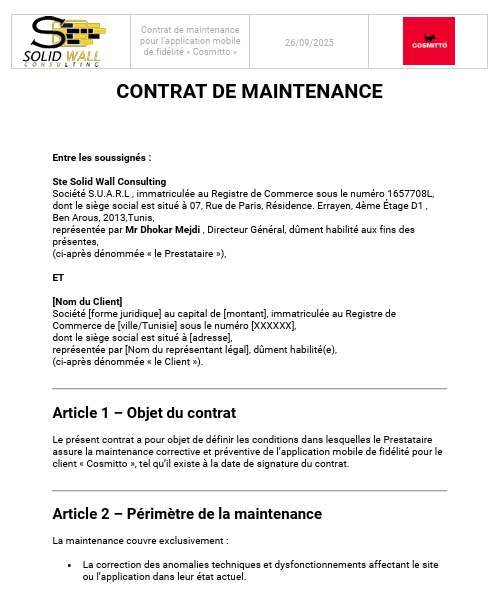
\includegraphics[width=\textwidth, keepaspectratio]{Images/Contrat1.png}
                    
                    \label{fig:contrat1}
                \end{subfigure}
                \hfill
                \begin{subfigure}[b]{0.45\textwidth}
                    \centering
                    
\includegraphics[width=\textwidth, keepaspectratio]{Images/contra2.png}
                    \label{fig:contrat2}
                \end{subfigure}
                \caption{Exemples de contrats de maintenance dans le système actuel}
                \label{fig:exemples_contrats}
            \end{figure}
            \noindent
            --\hspace{0.5cm} \textbf{Processus de gestion des demandes clients }
            \newline
            Le processus des demandes de maintenance repose actuellement sur des échanges via WhatsApp, des messageries instantanées ou des appels téléphoniques. Lorsque le client souhaite signaler un problème, il envoie un message décrivant sa demande au responsable concerné.
           \newline Afin de mieux illustrer ce mode de fonctionnement, la figure ci-dessous présente un exemple de traitement des demandes clients dans le système actuel.
            \begin{figure}[H]
   
    
    
        \centering
        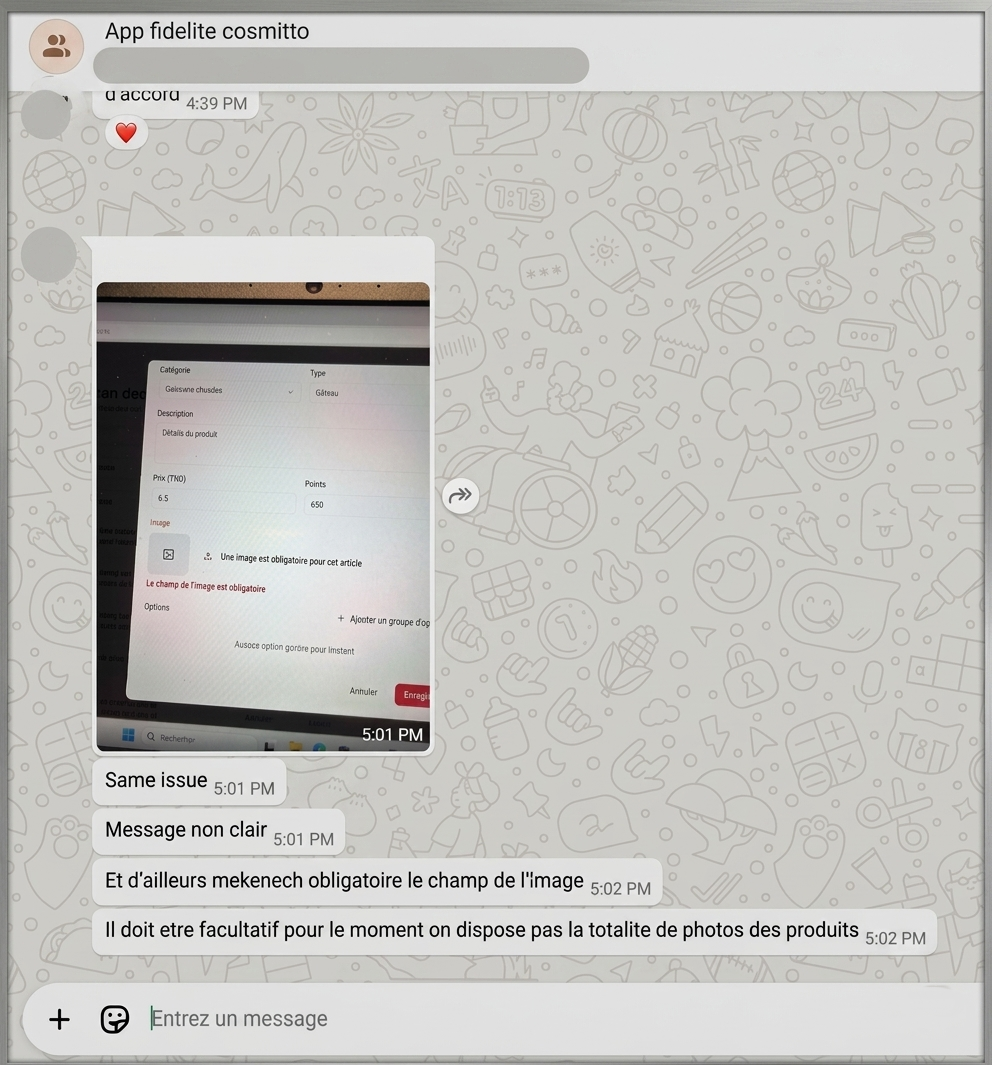
\includegraphics[width=0.40\linewidth, height=0.40\textheight, keepaspectratio]{Images/demande de maintenance.png}
        \caption{Demande de maintenance effectuée via l’application WhatsApp}
        \label{subfig:Demande de maintenance effectuée via l’application WhatsApp}
    \hfill

\end{figure}
\newpage
            \noindent
            --\hspace{0.5cm} \textbf{Processus de suivi des tickets de maintenance }
            \newline
Le suivi des interventions repose au quotidien sur des fils de discussion par e-mail, et l’affectation des tickets aux développeurs est assurée par le responsable, généralement via un message direct. 
\newline Afin d’illustrer plus concrètement ce processus, un exemple de rapport de test et de suivi des anomalies, consigné dans un fichier Excel où sont répertoriés les modules touchés, la description des problèmes rencontrés et leur statut, est présenté ci-dessous.
\begin{figure}[H]
    \centering
    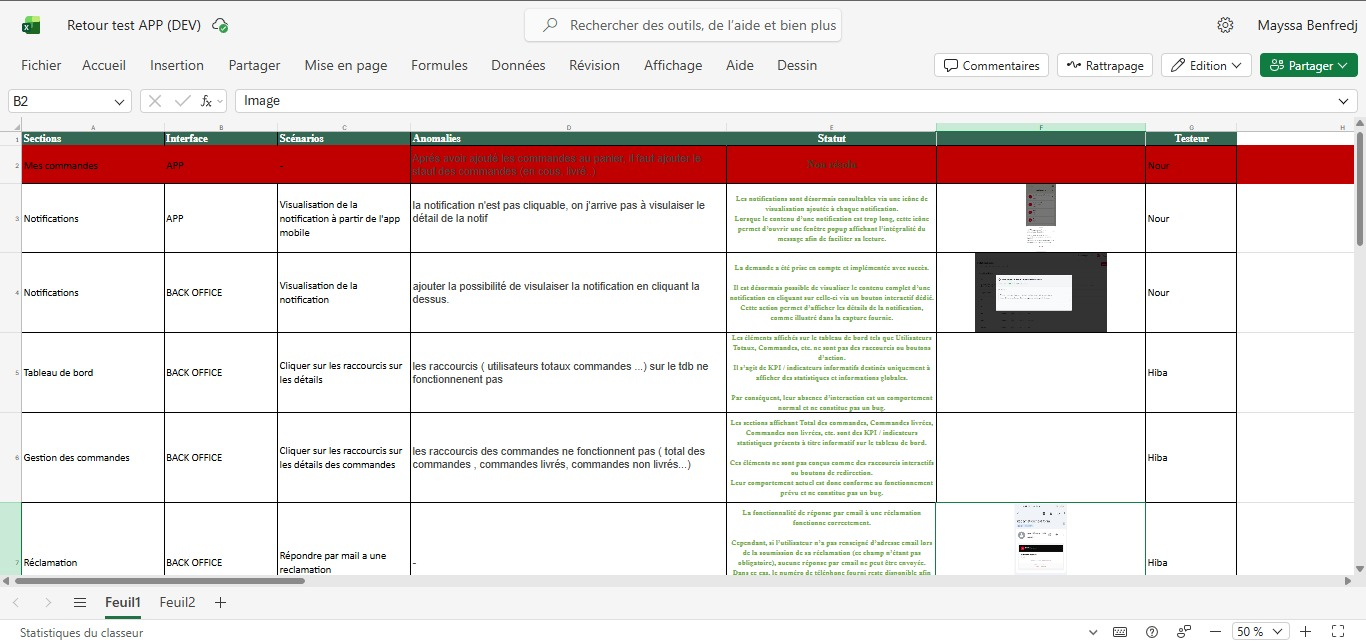
\includegraphics[width=0.80\textwidth, height=0.98\textheight, keepaspectratio]{Images/demande de maintenance sous format excel.png}
    \caption{Exemple de suivi des interventions à l’aide d’un fichier Excel}
    \label{subfig:excel}
\end{figure}
            --\hspace{0.5cm} \textbf{Processus de traçabilité des actions et des documents }
 \newline Les documents contractuels sont stockés dans des répertoires locaux ou sur des espaces de stockage cloud. Les fichiers sont organisés selon les pratiques de chaque responsable, et les modifications sont effectuées directement sur les documents existants.
            \newline

    \item  \textcolor{bleuPerso} {Étude de l'existant à l'échelle internationale}~\newline
            Avant de développer notre propre solution, nous allons étudier les solutions disponibles sur le marché afin d'analyser les fonctionnalités proposées. Cette démarche permet d'identifier les bonnes pratiques et d'orienter efficacement le développement de notre système.\newline
            Dans ce cadre, nous avons étudié plusieurs solutions existantes couvrant différents segments du marché : solutions open-source, solutions \textbf{SaaS} (\textit{Software as a Service}) et solutions enterprise.
\newpage
\noindent  --\hspace{0.5cm}  \textbf{GLPI (Gestionnaire Libre de Parc Informatique)}\par\smallskip
GLPI, lancée en 2003 et maintenue par l’éditeur français Teclib, est une solution open-source de référence pour la gestion des services informatiques et des infrastructures. Elle permet de gérer le parc informatique avec inventaire, licences et cycle de vie des actifs, tout en offrant un centre de services pour le traitement des incidents et des demandes, le suivi des SLA et le maintien d’une base de connaissances conforme aux bonnes pratiques \textbf{ITSM} (\textit{Information Technology Service Management}). La version communautaire est gratuite en on-premise sous licence GPLv3+, tandis que des abonnements payants sont disponibles pour un support cloud managé ou une assistance professionnelle. \cite{glpi} 
                    \begin{figure}[H]
                            \centering
                            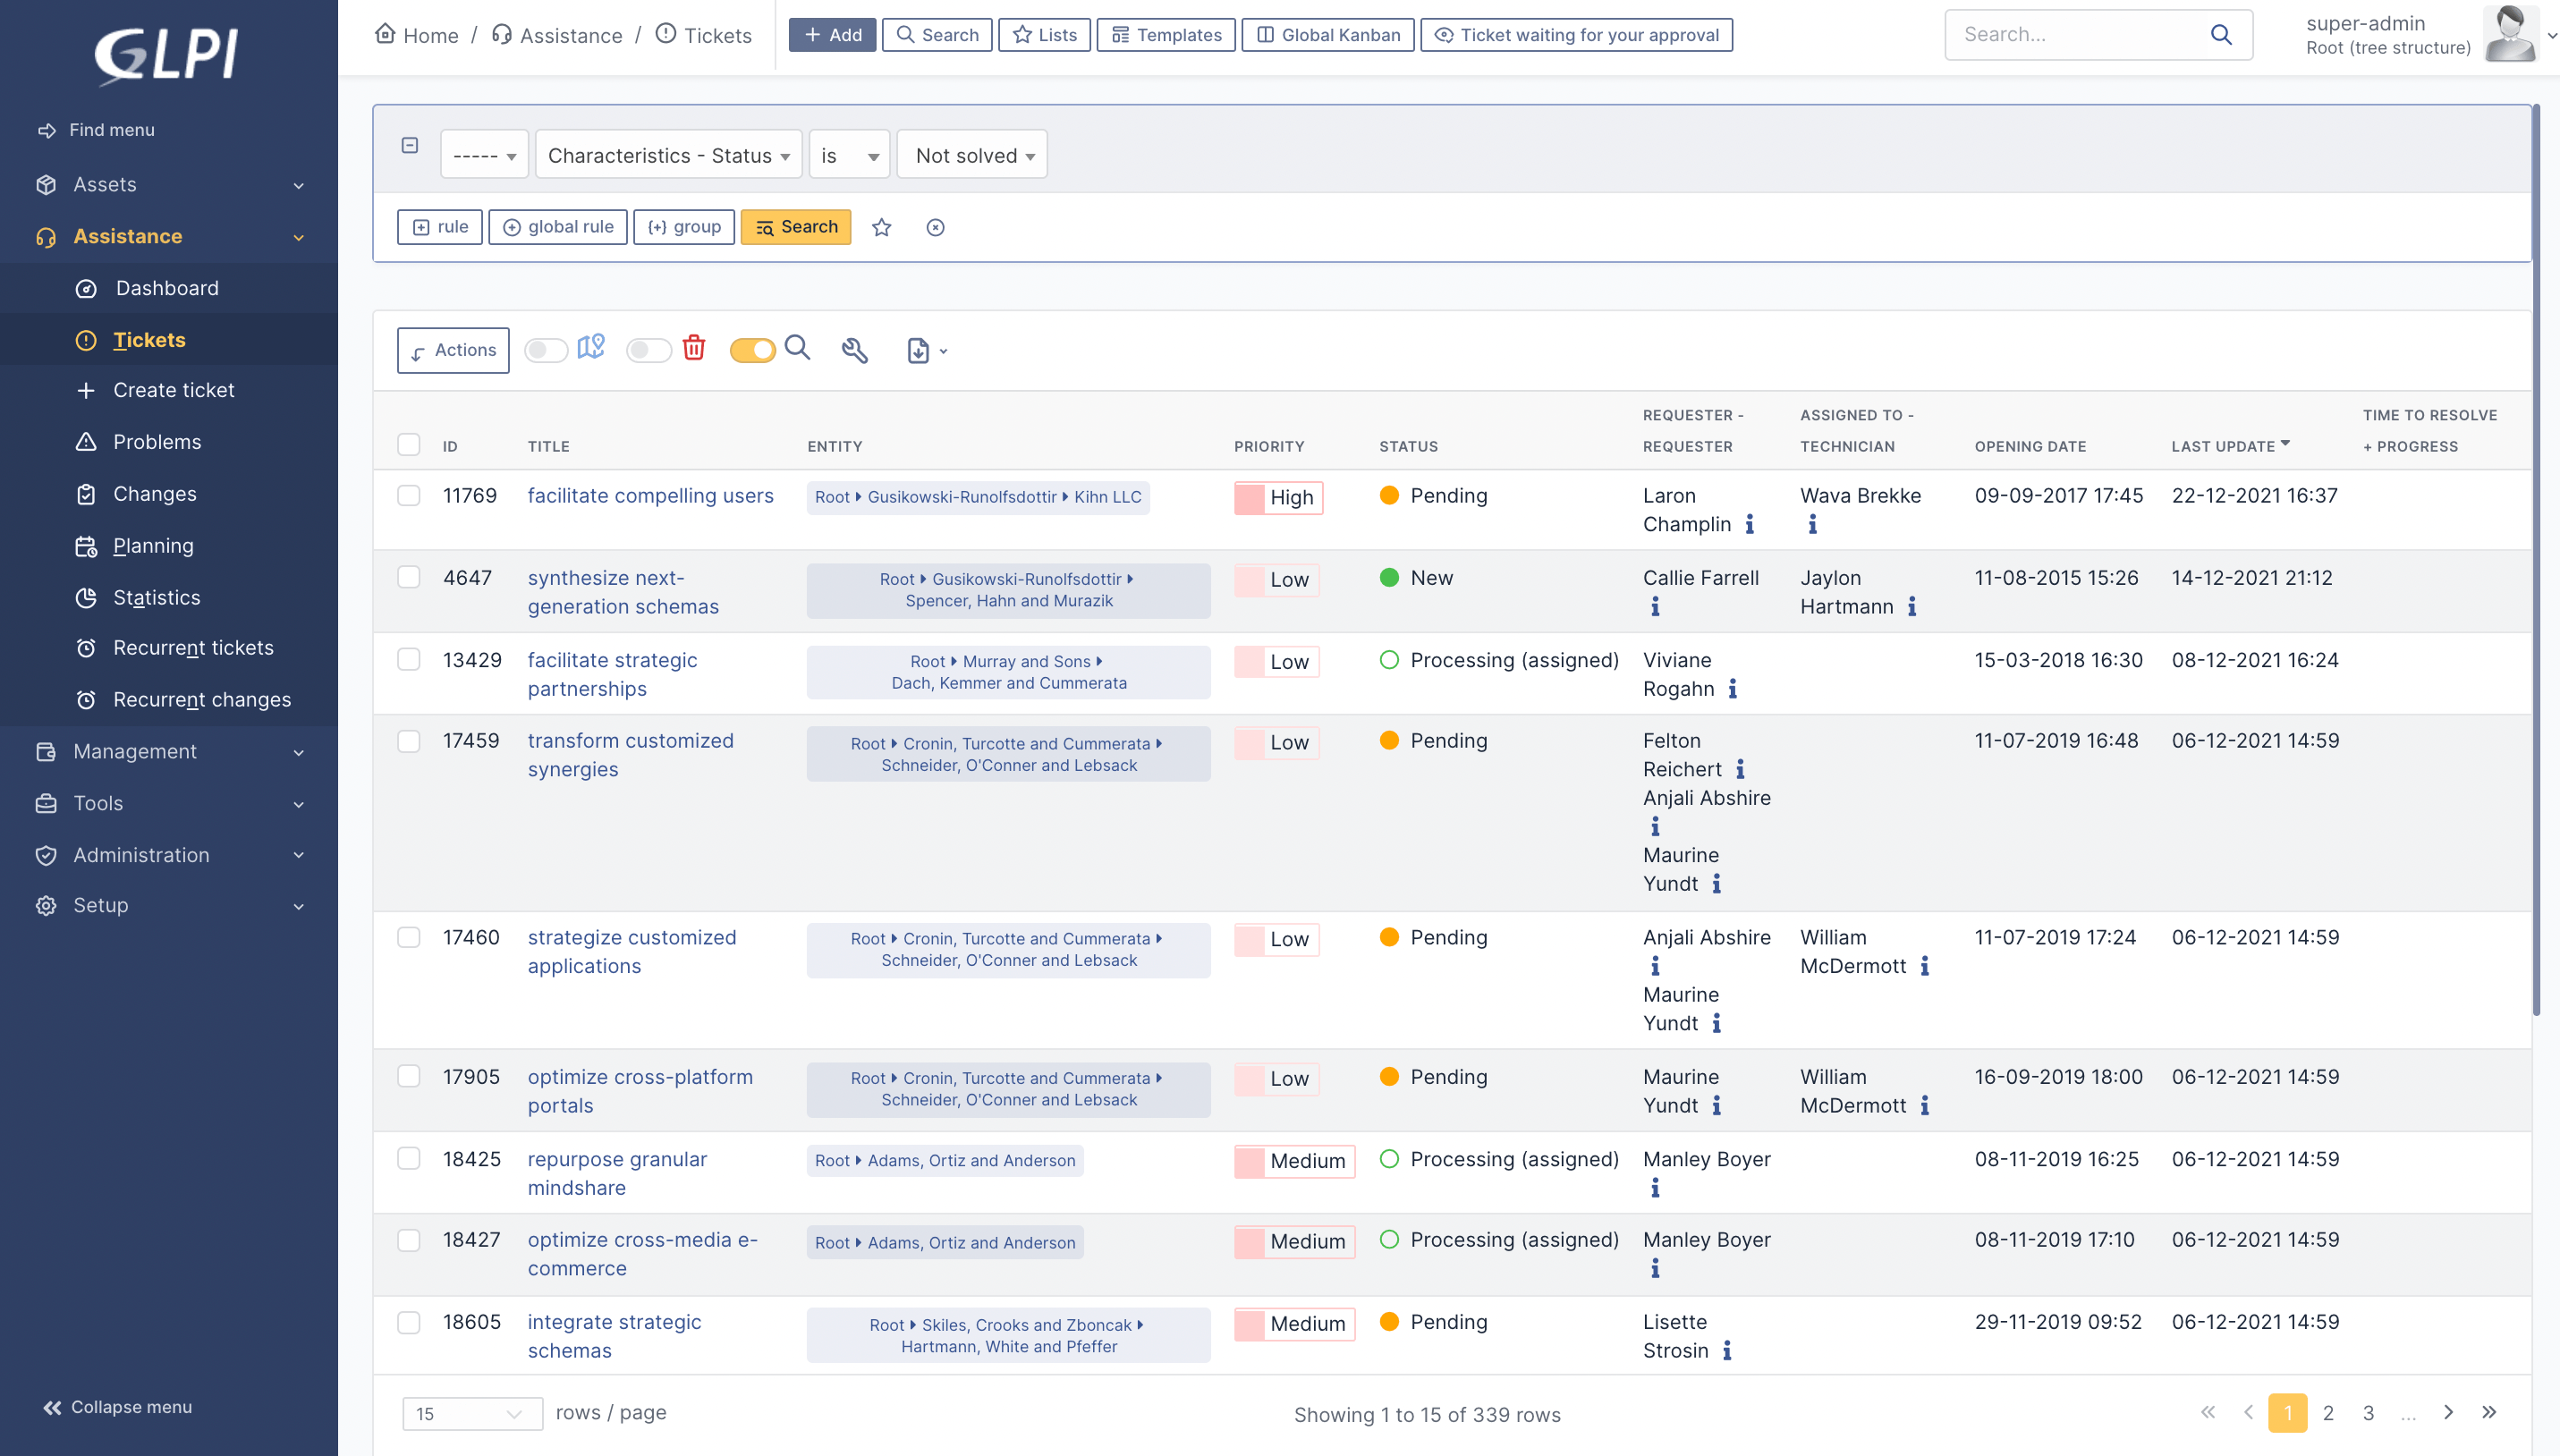
\includegraphics[width=0.7\textwidth,keepaspectratio]{Images/GLPI.png}
                            \caption{Interface de GLPI }
                            \label{fig:GLPI}
                        \end{figure}
  \vspace{0.4cm}
                  \noindent  --\hspace{0.5cm}  \textbf{Freshdesk}\par\smallskip
Freshdesk, créée en 2011 par Freshworks, s’impose comme une plateforme \textbf{SaaS} (\textit{Software as a Service}) de support client omnicanale capable de traiter les messages email, chat et réseaux sociaux tout en orchestrant une distribution intelligente des tickets et en enrichissant les interactions grâce à l'\textbf{IA} (\textit{Intelligence Artificielle}) Freddy AI. Cette solution conjugue la gestion des demandes, le suivi des SLA et l’automatisation des workflows pour améliorer la réactivité des équipes. Son modèle économique repose sur un principe freemium, avec un tarif de base à partir de 15~€/agent/mois et des options payantes pour des fonctionnalités avancées. \cite{freshdesk}                   
                    \begin{figure}[H]
                                        \centering
                            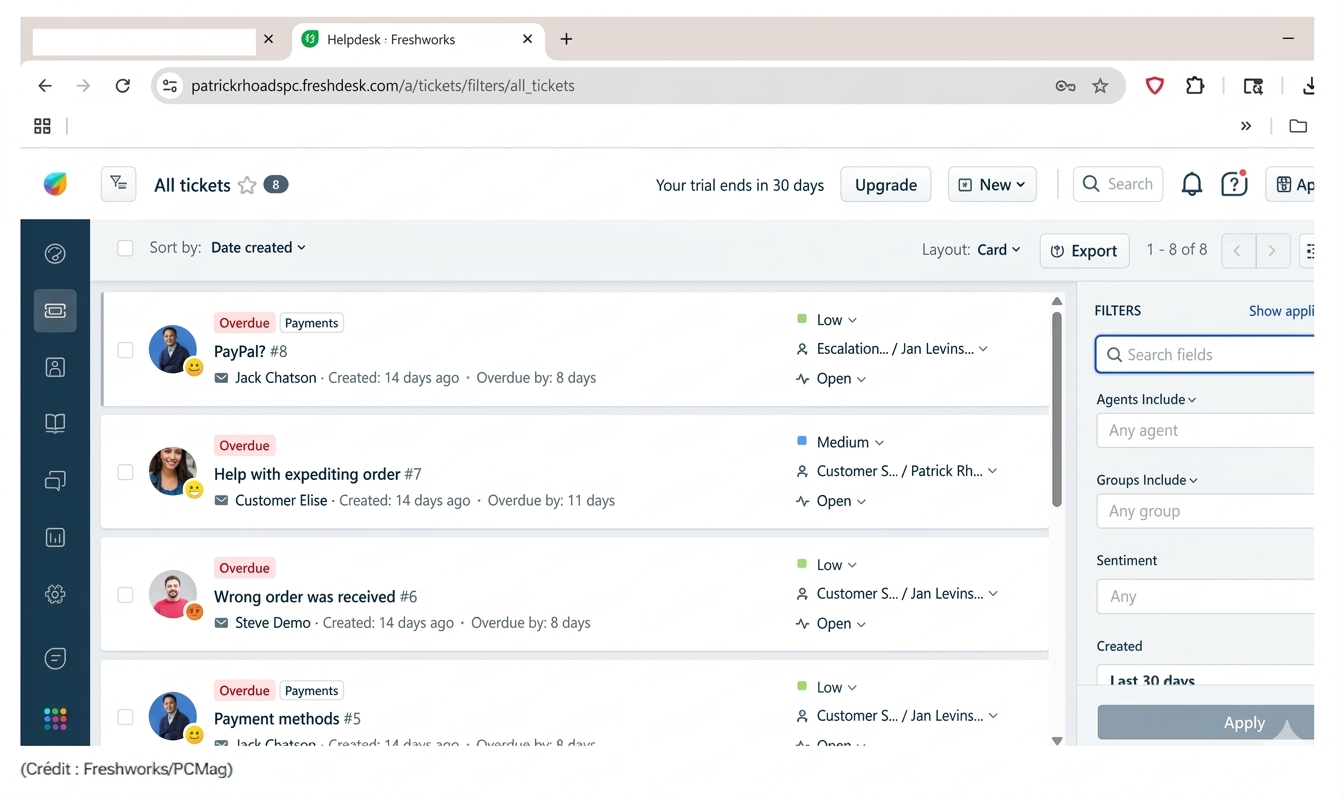
\includegraphics[width=0.7\textwidth,keepaspectratio]{Images/FreshDesk.png}
                            \caption{Interface de Freshdesk}
                            \label{fig:freshdesk}
                        \end{figure}
 \vspace{0.4cm}
                  \noindent --\hspace{0.5cm}  \textbf{Jira Service Management (Atlassian)}\par\smallskip
Jira Service Management, lancé en 2013 par Atlassian, propose un cadre ITSM (Information Technology Service Management) centré sur la gestion des incidents, des demandes et des changements, avec des tableaux de bord dédiés au suivi des engagements de service et des automatisations pour fluidifier les processus. Cette offre tire parti de l'écosystème Jira pour relier opérationnel et développement, ce qui facilite le pilotage des équipes et des actifs. Elle est distribuée principalement via un modèle d'abonnement \textbf{SaaS} (\textit{Software as a Service}), avec des versions cloud et des licences self-hosted pour les organisations qui préfèrent héberger leur solution en interne. \cite{jira-service-management}                    
                    \begin{figure}[H]
                        \centering
                        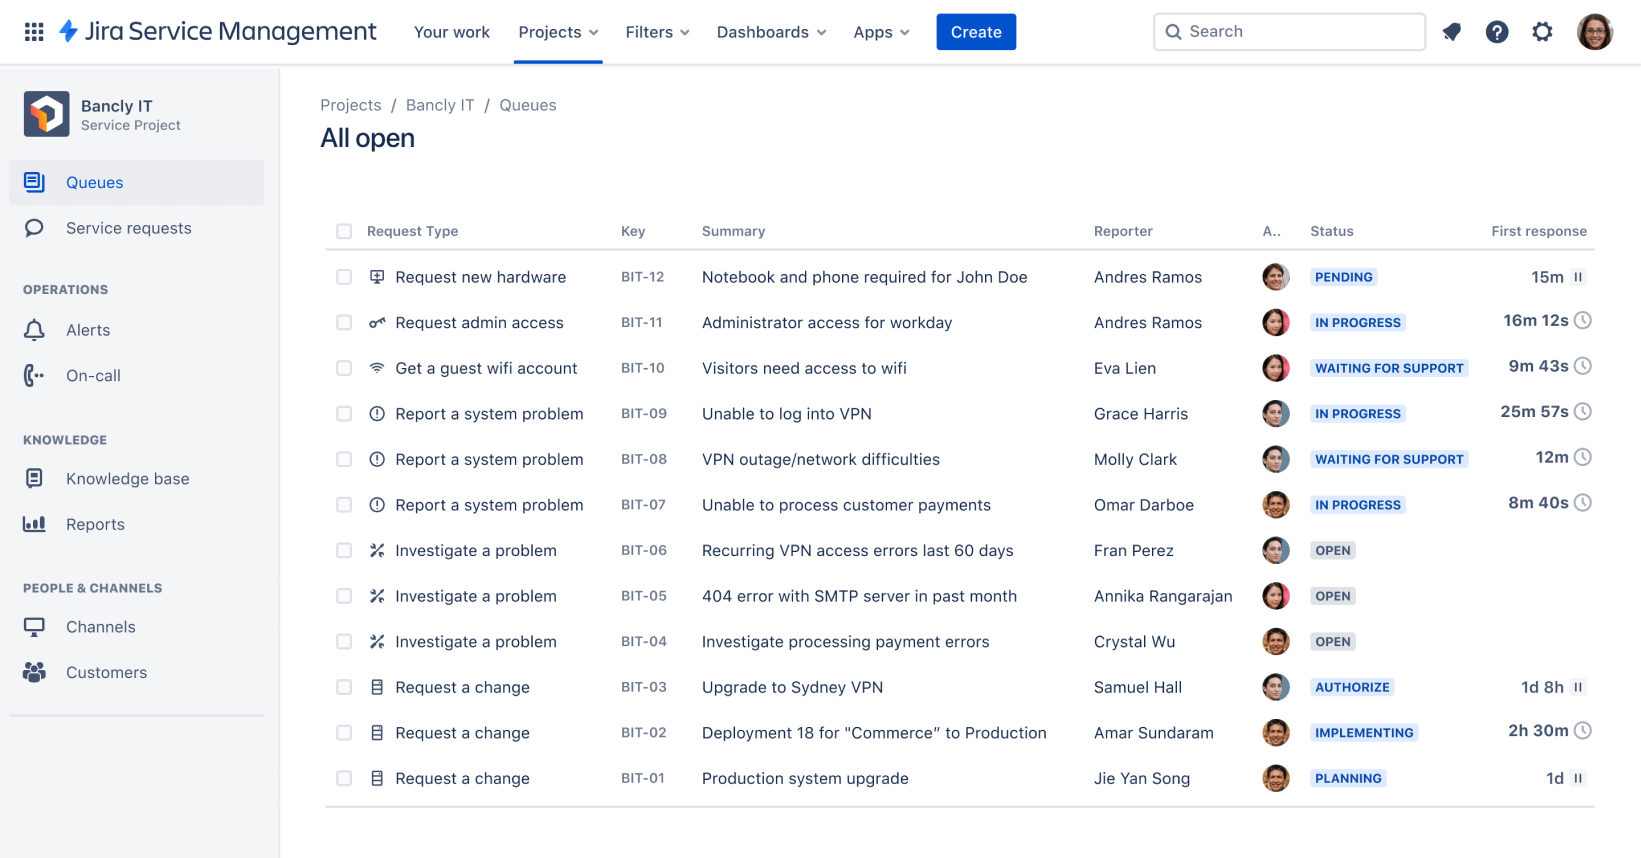
\includegraphics[width=0.7\textwidth,keepaspectratio]{Images/appJira.png}
                        \caption{Interface de Jira Service Management}
                        \label{fig:jira}
                    \end{figure}
            \noindent
\end{enumerate}


\subsubsection{Critique de l'existant}

Actuellement, la gestion des contrats de maintenance au sein de SolidWall Consulting repose sur un ensemble d'outils disparates : des documents Word pour les contrats, WhatsApp ou des courriels pour les demandes clients, et des fichiers Excel pour le suivi des interventions, sans système centralisé. Cette approche présente certaines limites.
\begin{enumerate}[label=\textcolor{bleuPerso}{\alph*)}, labelsep=0.5em]

 \item \noindent{\textbf{\textcolor{bleuPerso}{Limitations du processus actuel }}}
    \begin{itemize}[label=\ding{109}]
    \item \textbf{processus fragmenté : } La communication via e-mail fragmente la gestion. Les informations étant dispersées, le suivi des composants manquants devient complexe.  En l’absence de structure centralisée, il devient difficile de retrouver l'historique complet d'une intervention.
    \item \textbf{Absence de traçabilité :} L'absence de système de traçabilité rend le suivi des interventions difficile. Cela peut entraîner une perte de visibilité sur leur état, en cas de conflit avec un client ou lors d'un audit interne, ce qui représente un risque pour la crédibilité et la fiabilité de la société.
    \item \textbf{Risque de perte d'informations :} En raison de la fragmentation des processus, il existe un risque accru de perte d'informations importantes. Les documents sont stockés de manière non structurée, ce qui rend leur suivi et leur consolidation difficiles.
     \item \textbf{Complexité de la communication : } la communication au sein de l’équipe et avec les clients repose sur des échanges dispersés (courriels, messages), ce qui rend le flux des demandes peu clair et entraîne des retards dans le traitement des interventions.
    
    \end{itemize}

 \item \noindent{\textbf{\textcolor{bleuPerso}{Limitations des solutions existantes }}}
    \begin{itemize}[label=$\bullet$]
    \item \noindent\textbf{Complexité d'utilisation et courbe d'apprentissage}
    
    Les solutions existantes présentent une complexité d'usage importante. GLPI nécessite une formation de 2 à 3 jours pour les administrateurs avec une interface peu intuitive. Jira Service Management requiert une connaissance approfondie de l'écosystème Atlassian, créant une dépendance technique majeure.
    \newpage
    \item \noindent\textbf{Coût des licences et investissement financier}
    
    L'investissement financier représente un obstacle majeur pour l'adoption des solutions existantes. Les tarifs varient considérablement selon les offres : Freshdesk propose ses offres payantes à partir de 15€ par agent et par mois, tandis que Jira Service Management est tarifé à 20~€/agent/mois. GLPI, bien que gratuit en version communautaire, nécessite un minimum de 1500€ par an pour accéder au support entreprise. Pour une équipe de 10 utilisateurs, le coût annuel total s'élève ainsi à 1800€ pour Freshdesk, 2400€ pour Jira Service Management et 1500€ pour GLPI avec support.
    
    \item \noindent\textbf{Dépendance aux extensions et problèmes d'intégration}
    
    Les solutions du marché souffrent d'une architecture modulaire générant des coûts cachés. De nombreuses fonctionnalités avancées nécessitent des extensions payantes supplémentaires. Les mises à jour engendrent des problèmes de compatibilité, et l'intégration avec des systèmes existants nécessite souvent des développements spécifiques onéreux.
    \end{itemize}
\end{enumerate}
\subsubsection{Tableau comparatif des solutions}
\begin{table}[H]
    \centering
    \renewcommand{\arraystretch}{1.4}
    \arrayrulecolor{gray!70}
    \rowcolors{2}{gray!5}{white}
    \small
    \begin{tabularx}{\textwidth}{|>{\raggedright\arraybackslash}p{4cm}|>{\centering\arraybackslash}X|>{\centering\arraybackslash}X|>{\centering\arraybackslash}X|}
    \hline
    \rowcolor{blue!20}
    \textbf{Critères de comparaison} & \textbf{GLPI \cite{glpi}} & \textbf{Jira SM \cite{jira-service-management}} & \textbf{Freshdesk \cite{freshdesk}} \\
    \hline
    Gestion des tickets & \checkmark & \checkmark & \checkmark \\
    \hline
    Gestion des contrats \& SLA & Limité & Limité & $\times$ \\
    \hline
    Gestion de parc (Assets) & \checkmark & Limité (Payant) & $\times$ \\
    \hline
    Messagerie \& Chat intégré & Limité & Limité & \checkmark \\
    \hline
    IA \& Suggestions automatiques & $\times$ & \checkmark & \checkmark \\
    \hline
    Application \& Accès Mobile & Limité & \checkmark & \checkmark \\
    \hline
    Facilité d'utilisation & Moyenne & Moyenne & Facile \\
    \hline
    Coût indicatif (10 users / an) & 1500 € & 2400 € & 1800 € \\
    \hline
    \end{tabularx}
    \caption{Analyse comparative des solutions de gestion de maintenance du marché}
    \label{tab:comparaison_solutions}
\end{table}
\newpage
\smallskip
\noindent\textit{\textbf{Remarque sur les coûts} — Les tarifs annuels présentés pour 10 utilisateurs correspondent aux offres de base : 1~800~€/an pour Freshdesk, 2~400~€/an pour Jira SM, et 1~500~€/an pour le support entreprise de GLPI (dont la version communautaire reste gratuite). Ces montants excluent les fonctionnalités optionnelles, les supports premium et les frais de personnalisation.}
\subsubsection{Solution proposée}

C'est dans ce cadre que s'inscrit \textbf{SolidMaint}, une 
plateforme web intégrée visant à automatiser et à centraliser 
l'ensemble du processus de gestion des contrats de maintenance 
au sein de \textbf{SolidWall Consulting}. Elle s'articule 
autour de trois modules fonctionnels complémentaires :

\noindent\textbf{Module 1 : Gestion des Clients, Projets et Contrats}

Ce module centralise la gestion des clients, des projets et 
des contrats de maintenance. Il offre une visibilité complète 
sur les engagements contractuels par client et intègre un 
système d'alertes préventives permettant d'anticiper les 
échéances et de garantir le respect des accords de niveau 
de service (SLA).

\noindent\textbf{Module 2 : Gestion des Demandes et Tickets}

Ce module structure le cycle de vie complet des demandes 
clients, depuis leur soumission jusqu'à leur clôture. Il 
automatise la génération des tickets, facilite leur 
affectation aux développeurs compétents et assure un suivi 
précis du temps d'intervention, contribuant ainsi à une 
meilleure maîtrise des délais de résolution.

\noindent\textbf{Module 3 : Collaboration et Assistance 
Intelligente}

Ce module regroupe les fonctionnalités avancées de 
communication et d'intelligence artificielle, notamment 
la messagerie en temps réel, la gestion documentaire et 
les notifications multicanaux, afin de fluidifier les 
échanges entre les différents acteurs de la plateforme.

En réponse aux insuffisances identifiées, \textbf{SolidMaint} 
centralisera l'ensemble des processus de maintenance au sein 
d'un environnement unifié, fiable et évolutif, permettant à 
\textbf{SolidWall Consulting} d'améliorer sa réactivité et 
de renforcer la qualité de ses prestations.

\section{Choix du framework de gestion de projet}
\label{sec:methodologie}
Le choix méthodologique est déterminant pour la réussite d'un projet de développement. Une méthodologie appropriée structure le travail, optimise la gestion des ressources et garantit la qualité du livrable dans le respect des délais impartis.

\subsection{Méthodologie classique }
La méthodologie classique s'appuie sur une planification prédictive et une exécution séquentielle : chaque phase est définie au préalable, puis réalisée de l'analyse des besoins à la mise en production. Cette stratégie offre une maîtrise élevée des livrables, des délais et des coûts lorsque les exigences sont stables et que le périmètre évolue peu.

Cependant, cette rigidité expose le projet à des retours en arrière coûteux dès qu'une correction ou un nouveau besoin apparaît après la conception. Le cycle en V met en lumière cette logique en associant systématiquement chaque phase de conception à une phase de validation, ce qui privilégie la conformité au détriment de l'adaptabilité.\cite{brandenbourg-gestion}

\subsubsection{Principes de la méthodologie classique}
L'approche repose sur une progression linéaire où chaque étape sert de fondation à la suivante. Elle exige une définition détaillée des besoins en phase initiale et une validation formelle à chaque transition, ce qui limite la capacité d'adaptation en cas de changement ultérieur.



\subsection{Méthodologie Agile}
L'approche agile s'appuie sur une progression itérative et sur l'apprentissage continu. Plutôt que de figer l'ensemble du périmètre en début de projet, elle privilégie des cycles de travail courts qui permettent de valider des fonctionnalités opérationnelles et de réajuster les priorités selon les retours métiers. Cette dynamique permet au projet de rester proche des attentes des utilisateurs et de limiter les écarts entre les besoins réels et les livrables.

Dans le contexte de SolidMaint, l'agilité renforce la capacité à intégrer rapidement de nouvelles demandes ou des corrections, tout en maintenant un rythme de livraison régulier. Ce mode de travail favorise une collaboration étroite entre l'équipe de développement, le Product Owner et les parties prenantes, et transforme le changement en levier  \newline d'amélioration plutôt qu'en source de retard. \cite{agile-manifesto}




\subsubsection{Choix de l’approche Agile}
Le domaine de la maintenance impose des besoins imprévisibles, excluant toute planification rigide. Nous adoptons donc une approche agile basée sur la simplicité afin de produire l'essentiel efficacement. Pour cela, nous avons choisi la méthode Scrum, qui s'impose comme le cadre itératif idéal pour livrer rapidement de la valeur tout en restant réactifs aux changements.
\subsubsection{ Les principales méthodes Agiles}
Le tableau suivant met en évidence les méthodes Agile les plus couramment utilisées, selon différents critères de comparaison.
\begin{table}[H]
    \centering
    \renewcommand{\arraystretch}{1.6} % Espace vertical pour aérer les cellules
    
    % Couleur des bordures et alternance des couleurs de lignes
    \arrayrulecolor{gray!70}      
    \rowcolors{2}{gray!5}{white} 
    
    \begin{tabularx}{\textwidth}{
        | >{\bfseries\raggedright\arraybackslash}p{3.5cm} 
        | >{\centering\arraybackslash}X 
        | >{\centering\arraybackslash}X 
        | >{\centering\arraybackslash}X 
        | }
        
    \hline
    \rowcolor{blue!20} \textbf{Critères} & \textbf{Scrum} & \textbf{Kanban} & \textbf{Extreme Programming (XP)} \\
    \hline
    Type de projet & Incrémental & Continu & Technique \\
    \hline
    Critère d'évaluation & Vélocité & Fluidité & Qualité \\
    \hline
    Gestion des risques & Détection & Visualisation & Prévention \\
    \hline
    Implication client & Ponctuelle & Variable & Très forte et continue \\
    \hline
    
\end{tabularx}
    \vspace{0.2cm}
    \caption{Les principales méthodes Agiles.}
    \label{tab:methodes_agiles}
\end{table}

\subsubsection{Choix de la méthode Scrum}
Scrum a été retenue comme cadre de travail pour structurer le développement en itérations courtes tout en s'adaptant aux changements fréquents. Cette méthode offre plusieurs avantages décisifs :
\newline
\noindent
         --\hspace{0.5cm} Collaboration continue entre l'équipe et les parties prenantes
\newline --\hspace{0.5cm}  Adaptation rapide aux changements grâce aux cycles itératifs
\newline --\hspace{0.5cm} Livraisons régulières de fonctionnalités opérationnelles
\newline --\hspace{0.5cm} Détection précoce des problèmes et ajustements immédiats
\newline --\hspace{0.5cm} Transparence totale sur l'avancement du projet

\begin{figure}[H]
        \centering
        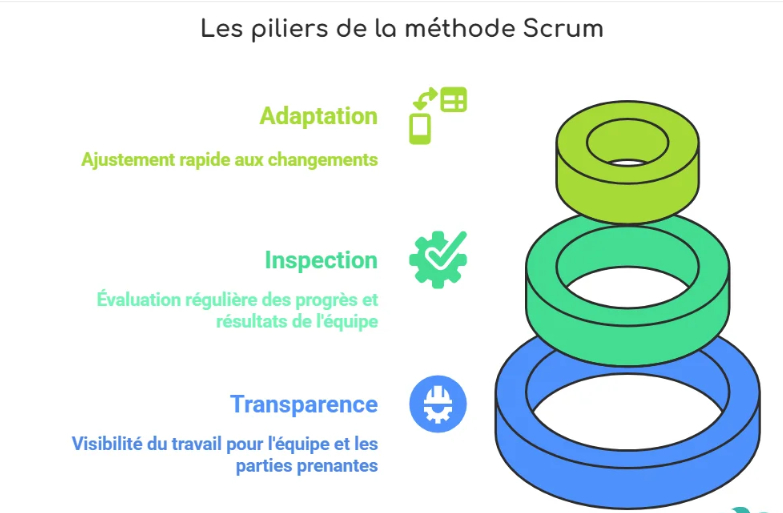
\includegraphics[width=0.7\textwidth,keepaspectratio]{Images/les piliers de la methodologie.png}
        \caption{les piliers de la méthode Scrum}
        \label{fig:les piliers de la méthode Scrum}
\end{figure}

\subsection{Fondements de SCRUM }
Scrum est un cadre organisationnel qui structure le développement itératif par successifs cycles courts appelés sprints, généralement étalés sur 2 à 4 semaines. Ce modèle s'appuie sur l'expression des besoins sous forme d'items de travail (user stories) ordonnancés et priorisés, permettant une livraison régulière de valeur métier mesurable et exploitable. La philosophie sous-jacente vise à concilier productivité de l'équipe et satisfaction continue du client par l'ajustement perpétuel. 

Scrum repose sur trois piliers fondamentaux qui constituent sa colonne vertébrale : la \textbf{transparence} crée une visibilité partagée et incontestable sur la progression réelle du travail, les risques et les décisions ; l'\textbf{inspection} encourage l'évaluation critique et régulière des artefacts (produit, processus, incrément) pour identifier rapidement tout écart ou opportunité ; enfin, l'\textbf{adaptation} autorise l'équipe à réviser son approche, ses priorités et ses méthodes en réaction directe aux faits observés et aux retours des parties prenantes.\cite{scrum-guide}

\subsection{Rôles de SCRUM}
La structure organisationnelle de Scrum s'appuie sur trois rôles qui répartissent clairement les responsabilités entre le pilotage métier, la facilitation du cadre et la réalisation technique.

\subsubsection{Product Owner}
Le Product Owner est responsable de la valeur métier du produit et de la vision métier du projet. Il définit les exigences de l’application et priorise les éléments du Product Backlog en fonction des objectifs de la société.
\subsubsection{Scrum Master}
Le Scrum Master est le garant du cadre Scrum. Il veille à ce que les pratiques agiles soient respectées, facilite les événements et aide à lever les obstacles qui freinent l’équipe.
\subsubsection{Les développeurs}
L’équipe de développement est chargée de la réalisation opérationnelle : conception, configuration,
développement et tests. Elle transforme les besoins priorisés en incréments fonctionnels prêts à être validés.

\subsection{Événements Scrum}
Les événements Scrum constituent des points de synchronisation structurés qui rythment l'exécution, entretiennent la discipline itérative, et incarnent les trois piliers de transparence, d'inspection et d'adaptation. Chaque événement possède une durée maximale prescrite et sert un objectif métier bien défini.
\begin{itemize}[nosep, left=0pt, label=\textbullet]
\item \textbf{Sprint~:} Conteneur itératif d'une durée fixe (généralement 2 à 4 semaines) au cours duquel l'équipe s'engage à livrer un incrément potentiellement commercialisable du produit. Chaque sprint débute par une planification et s'achève par une revue et une rétrospective.
\item \textbf{Sprint Planning~:} Événement de lancement où l'équipe et le Product Owner se rencontrent pour définir l'objectif du sprint et sélectionner les éléments du Product Backlog jugés réalisables. Cet atelier établit le Sprint Backlog et fixe les attentes de livrables.
\item \textbf{Daily Scrum (ou Mêlée quotidienne)~:} Synchronisation brève de 15 minutes maximum où l'équipe revient sur ses accomplissements, anticipe les travaux prévus et signale les obstacles rencontrés. Cet instant de transparence quotidienne renforce cohésion et réactivité.
\item \textbf{Sprint Review~:} Présentation et démonstration du travail accompli durant le sprint devant les parties prenantes. Elle permet la collecte de retours formels et l'ajustement du Product Backlog selon les commentaires et les besoins révisés.
\item \textbf{Sprint Retrospective~:} Moment d'introspection où l'équipe analyse collectivement son fonctionnement, met en lumière réussites et difficultés, et décide d'actions concrètes pour l'amélioration continue des futurs sprints.
\end{itemize}

\subsection{Artéfacts Scrum}
Les artéfacts Scrum matérialisent et expriment le travail, la valeur livrée et l'avancement du projet. Ils constituent des vecteurs de transparence et de communication pour tous les acteurs.
\begin{itemize}[nosep, left=0pt, label=\textbullet]
\item \textbf{Product Backlog~:} Inventaire dynamique et ordonné de tous les besoins, fonctionnalités, corrections et tâches à réaliser. Maintenu et priorisé par le Product Owner selon retours clients et valeur métier, il évolue constamment et reflète l'état réel du produit visé.
\item \textbf{Sprint Backlog~:} Projection du Product Backlog pour le sprint en cours, sélectionné collectivement lors de la planification. Il formalise l'engagement de l'équipe sur les éléments à livrer et constitue la source unique de vérité pour le travail en cours.
\item \textbf{Incrément du Produit~:} Somme des éléments du Product Backlog finalisés au cours du sprint actuel et de tous les sprints précédents. Il représente une version cohérente, intégrée et testée du produit, offrant une valeur tangible et démontrée au destinataire. Seul un incrément répondant aux critères d'acceptation est comptabilisé.
\end{itemize}
\subsection{Cycle de vie}
    Le cycle de vie Scrum se compose de sprints successifs, chacun comprenant une planification, le développement, des réunions quotidiennes, une revue et une rétrospective. Ce processus itératif permet d'adapter le produit en continu aux besoins du client et d'améliorer l'équipe à chaque itération.

    \begin{figure}[H]
        \centering
        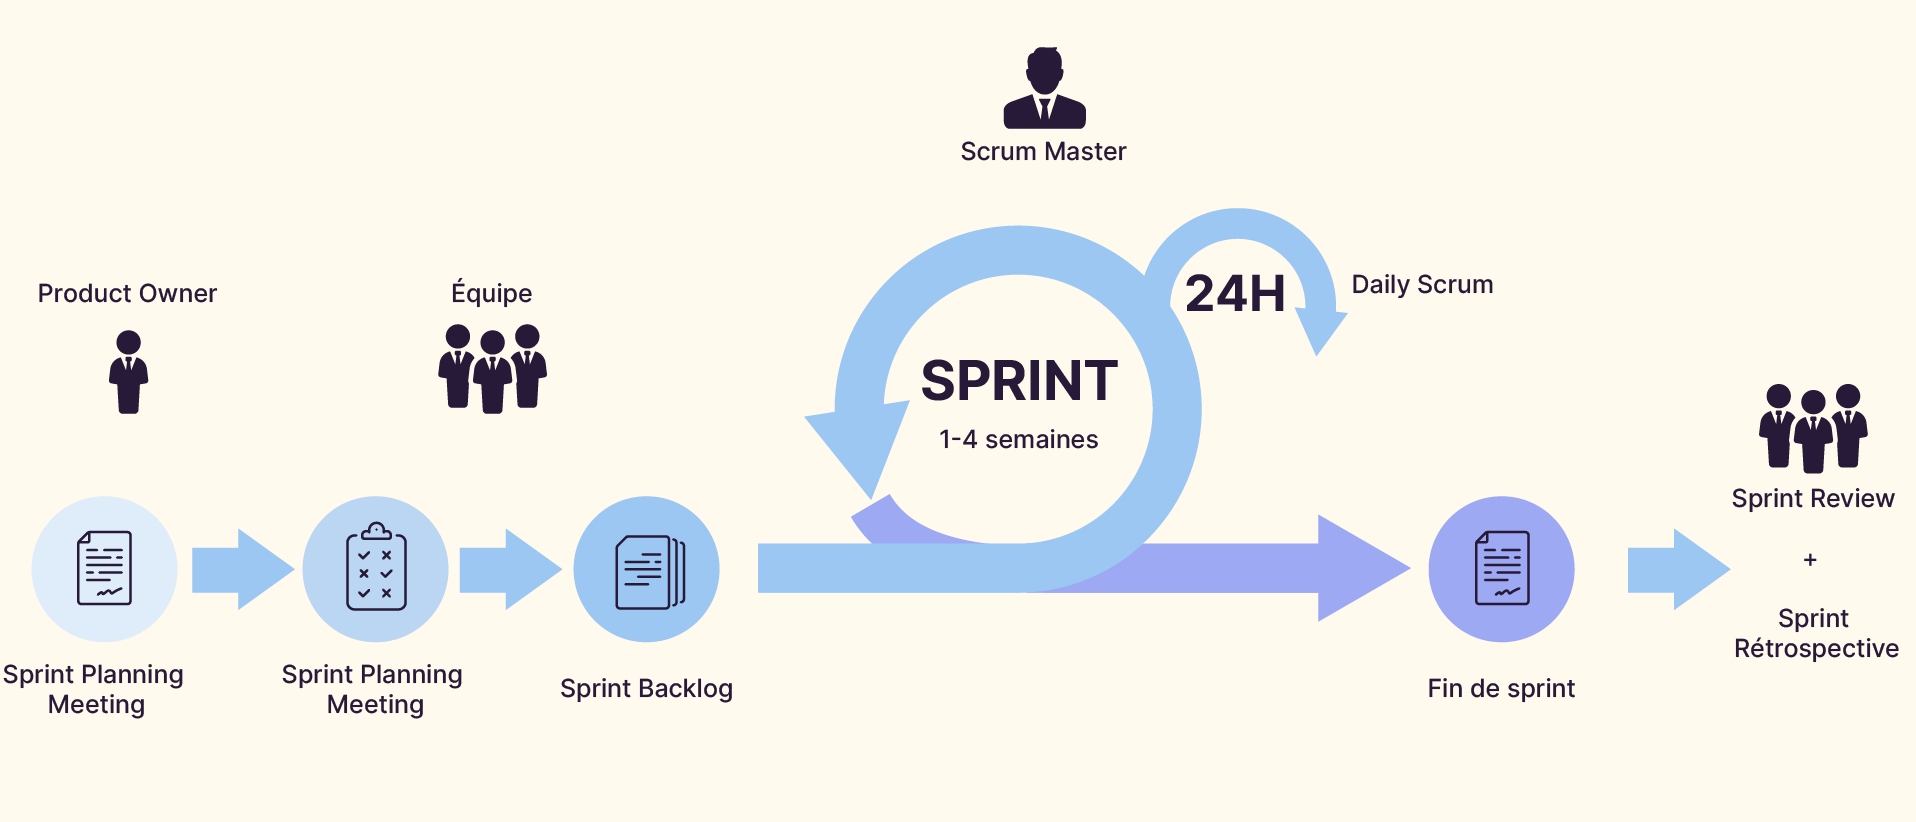
\includegraphics[width=0.75\textwidth,keepaspectratio]{Images/processus_scrum.png}
        \caption{Cycle de vie Scrum}
    \end{figure}
    
   
\section{Langage de modélisation UML}
« Le langage de modélisation unifié (UML) est un langage permettant de spécifier, visualiser, construire et documenter les artefacts des systèmes logiciels, ainsi que de modéliser des systèmes métier et d'autres systèmes non logiciels. L'UML représente un ensemble de bonnes pratiques d'ingénierie qui ont fait leurs preuves dans la modélisation de systèmes vastes et complexes. » \cite{omg-uml-importance}

\begin{figure}[H]
        \centering
        
\includegraphics[width=0.4\textwidth,keepaspectratio]{Images/UML.png}
        \caption{Logo UML}
    \end{figure}
    Pour concevoir notre application, nous avons choisi UML comme langage de modélisation. Ce choix s'appuie sur plusieurs points forts tels que la communication entre l'équipe et la cohérence architecturale qui se fait de manière simplifiée et standardisée.
\section*{Conclusion}
    Ce chapitre a établi le cadre général de notre projet \textbf{SolidMaint} en présentant l'organisme d'accueil SolidWall Consulting et en analysant les enjeux de la gestion des contrats de maintenance. L'étude critique de l'existant a révélé des limitations significatives dans les processus actuels, tandis que l'analyse comparative des solutions du marché a confirmé la pertinence de développer une solution sur mesure.
    La solution \textbf{SolidMaint} proposée répond à ces défis par une approche intégrée centralisant l'ensemble du cycle de vie des contrats. L'adoption de la méthodologie Scrum et la planification en quatre sprints garantissent une approche itérative et collaborative pour la réalisation du projet.
    \newline Le chapitre suivant détaillera la spécification des besoins et la modélisation de la solution.



% ---- Chapitre 2 ----
\hiddenpart{Préparation du projet}
\chaptercover{2}{Préparation du projet}
\section*{Introduction}
Ce chapitre présente l'analyse et la spécification des besoins de notre plateforme
\textbf{SolidMaint}. Nous identifierons les acteurs du système et leurs besoins
fonctionnels et non fonctionnels, puis procéderons à la modélisation UML. Nous
détaillerons ensuite l'approche de pilotage Scrum avec la planification des sprints,
et présenterons l'environnement de développement ainsi que l'architecture technique
de l'application.

\section{Spécification des besoins}
\label{sec:specification_besoins}
L'étape de spécification des besoins est importante pour prouver qu'un besoin réel
existe, elle permet de définir explicitement les objectifs à atteindre.
\newline
Pour cela nous allons identifier les acteurs, leurs besoins fonctionnels et les
besoins non fonctionnels.

\subsection{Identification des acteurs}
Un acteur représente une personne, une organisation ou un autre système qui interagit
avec le système. Notre projet identifie six acteurs principaux :

\begin{table}[h!]
\centering
\renewcommand{\arraystretch}{1.4}
\begin{tabularx}{\textwidth}{|>{\raggedright\arraybackslash}p{0.28\textwidth}
                              |>{\raggedright\arraybackslash}X|}
\hline
\rowcolor{blue!20}\textbf{Acteur} & \textbf{Rôle} \\
\hline
Visiteur      & Soumet une demande de création de compte via OAuth (Google, GitHub)
                et attend la validation par un administrateur. \\
\hline
Utilisateur   & Accède aux fonctionnalités communes : authentification, gestion du
                profil, notifications multicanaux et historique d'activités. \\
\hline
Client        & Soumet des demandes de maintenance, consulte l'état d'avancement
                de ses tickets, accède à ses contrats et communique avec l'équipe
                projet via la messagerie intégrée. \\
\hline
Développeur   & Traite les tickets assignés, gère le chronomètre de travail, signale
                les blocages, propose des solutions et consulte la base de
                connaissances. \\
\hline
Chef de projet & Valide les demandes clients, assigne les tickets aux développeurs,
                 supervise le respect des SLA, gère les équipes et génère les
                 procès-verbaux. \\
\hline
Administrateur & Gère les utilisateurs, rôles, permissions, clients, projets et
                 contrats. Configure les SLA, supervise les tableaux de bord et
                 administre l'ensemble du système. \\
\hline
\end{tabularx}
\caption{Acteurs du système SolidMaint et leurs rôles}
\label{tab:acteurs}
\end{table}

\begin{figure}[H]
\centering
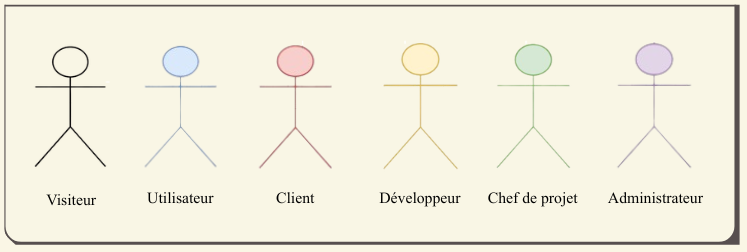
\includegraphics[width=0.9\textwidth,keepaspectratio]{Images/acteurs.png}
\caption{Illustration des acteurs du système SolidMaint}
\label{fig:acteurs}
\end{figure}

\subsection{Identification des besoins fonctionnels}
L'identification des besoins fonctionnels constitue une étape fondamentale dans la
conception de \textbf{SolidMaint}. Ces spécifications définissent précisément les
opérations que la plateforme doit être capable d'exécuter pour répondre aux exigences
métier de SolidWall Consulting.

\subsubsection{Authentification et Gestion de Compte}

Ce module assure l'authentification sécurisée via identifiants classiques ou OAuth 2.0 (Google, GitHub) avec gestion automatique des jetons d'accès. Lors de la première connexion, le système impose un changement de mot de passe pour les comptes créés par un administrateur. Un processus de réinitialisation obligatoire bloque l'accès à l'application jusqu'à la définition d'un mot de passe personnel, garantissant que seul l'utilisateur légitime détient les informations d'authentification définitives.

\begin{figure}[H]
    \centering
    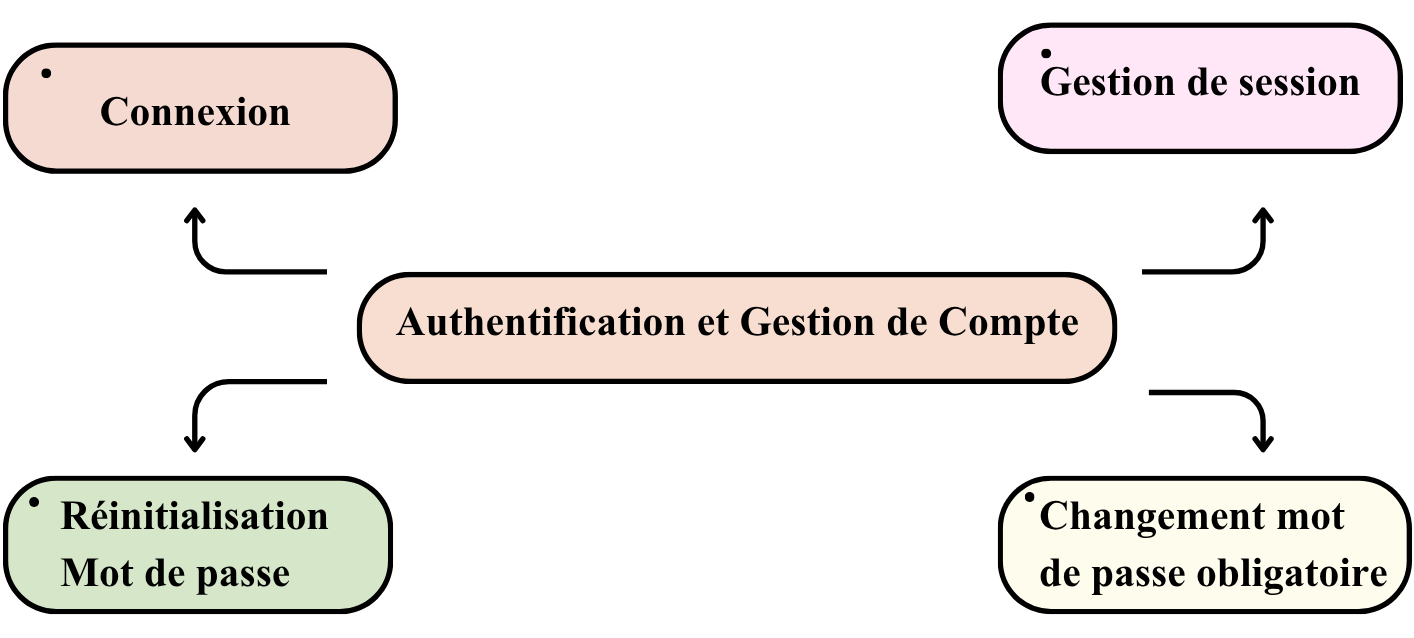
\includegraphics[width=0.7\textwidth,keepaspectratio]{Images/soumission_demande_inscription.png}
    \caption{Authentification et Gestion de Compte}
    \label{fig:authentification_gestion_compte}
\end{figure}

\vspace{0.5cm}

\subsubsection{Gestion des Utilisateurs et Demandes d'Inscription}

Ce module permet aux administrateurs de gérer le cycle de vie complet des comptes utilisateurs avec création automatisée, gestion des profils et contrôle des activations/désactivations. Le traitement des demandes d'inscription s'effectue via une interface centralisée permettant approbation, rejet ou mise en attente avec notifications automatiques.

\begin{figure}[H]
    \centering
    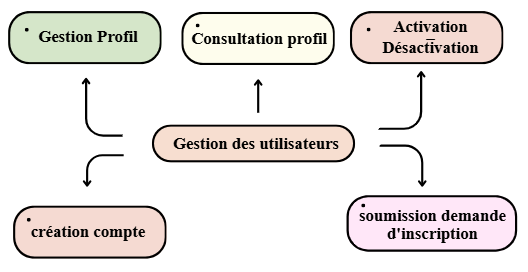
\includegraphics[width=0.7\textwidth,keepaspectratio]{Images/inscription_creation_utilisateur.png}
    \caption{Gestion des Utilisateurs et Demandes d'Inscription}
    \label{fig:gestion_utilisateurs}
\end{figure}

\vspace{0.5cm}

\subsubsection{Système de Rôles et Permissions}

Les droits sont gérés par rôles selon un modèle RBAC (Role-Based Access Control) : chaque rôle regroupe un ensemble de permissions, ce qui permet d’attribuer finement les accès. La conception modulaire permet aux administrateurs de créer des rôles personnalisés en combinant dynamiquement les permissions existantes selon les besoins organisationnels spécifiques. Cette flexibilité permet d'ajuster les autorisations d'un rôle sans impact sur les autres configurations, facilitant l'évolution du système de sécurité.

\begin{figure}[H]
    \centering
    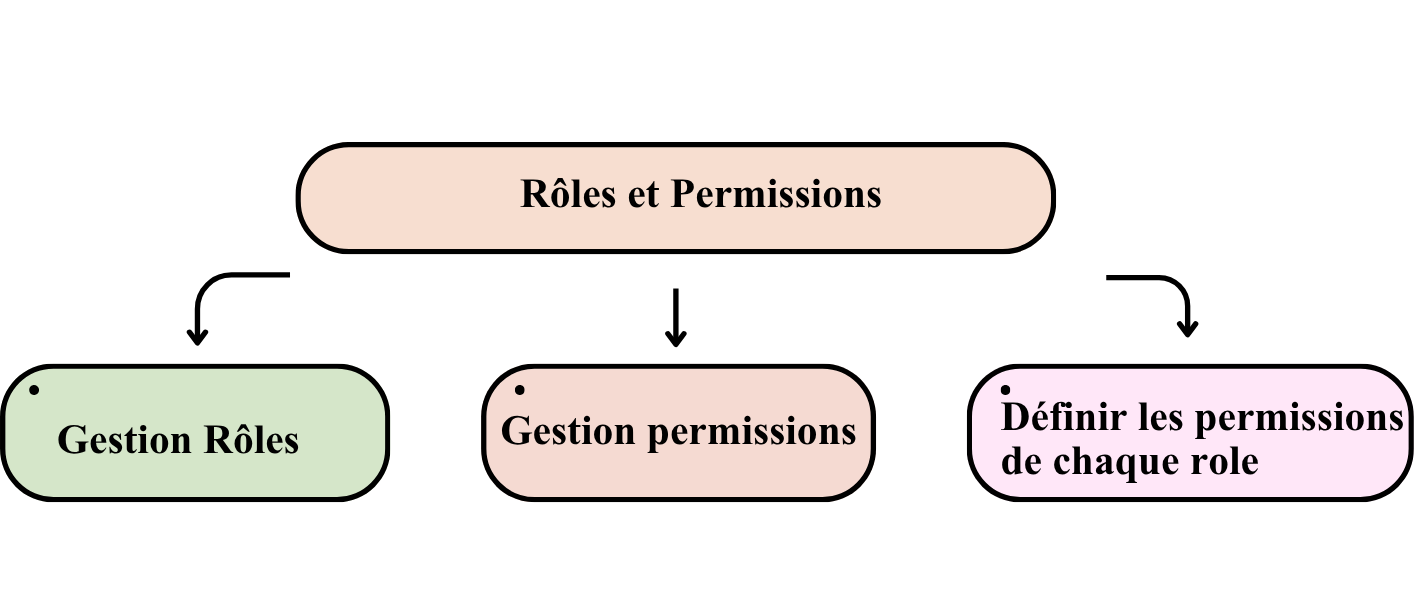
\includegraphics[width=0.7\textwidth,keepaspectratio]{Images/gestion_permissions.png}
    \caption{Système de Rôles et Permissions}
    \label{fig:roles_permissions}
\end{figure}

\vspace{0.5cm} 

\subsubsection{Gestion des Clients et Projets}

Ce module centralise la gestion des clients avec création automatisée des comptes. Le système génère des organigrammes visuels et interactifs pour chaque projet, présentant la hiérarchie complète (client, chef de projet, équipe) avec accès direct aux coordonnées de tous les interlocuteurs. Cette visualisation facilite l'identification rapide des contacts et optimise la communication en cas de problème.

\begin{figure}[H]
    \centering
    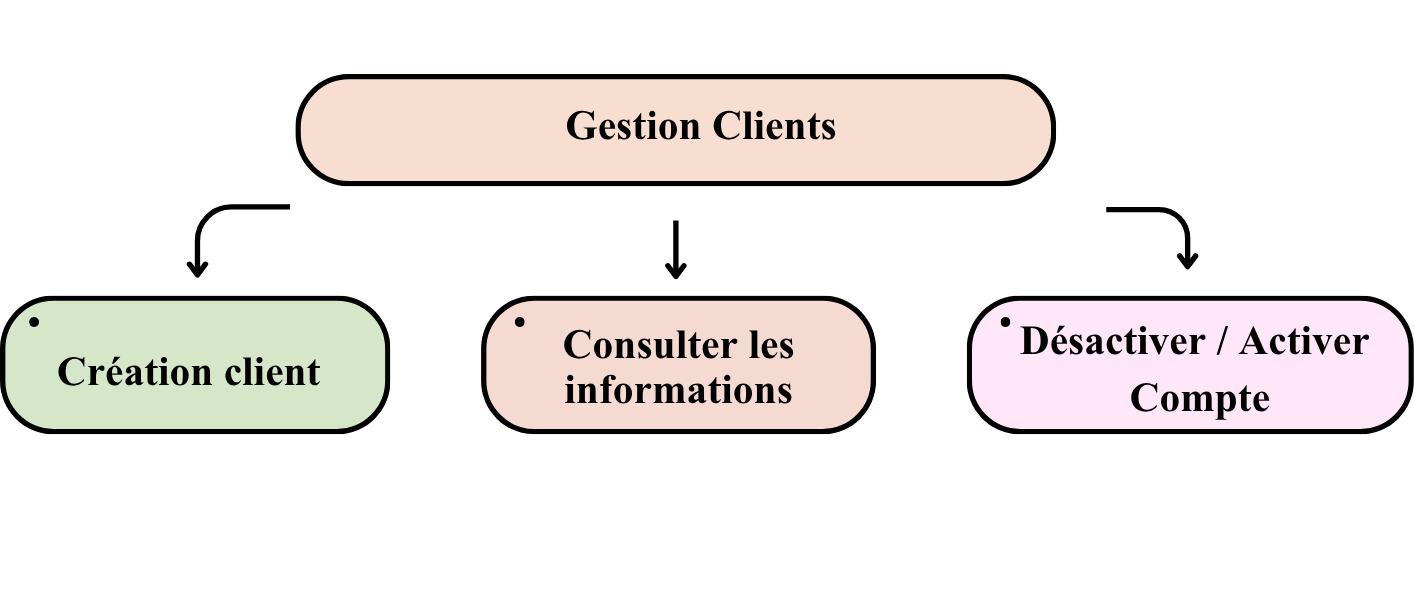
\includegraphics[width=0.7\textwidth,keepaspectratio]{Images/gestion_client.png}
    \caption{Gestion des Clients et Projets}
    \label{fig:gestion_clients}
\end{figure}

\subsubsection{Gestion des Contrats de Maintenance}

Ce module automatise le cycle de vie complet des contrats de maintenance avec système d'alertes préventives échelonnées. L'import de contrats s'effectue à partir de fichiers PDF, avec extraction automatique de données pour pré-remplir les formulaires de création.
\begin{figure}[H]
    \centering
    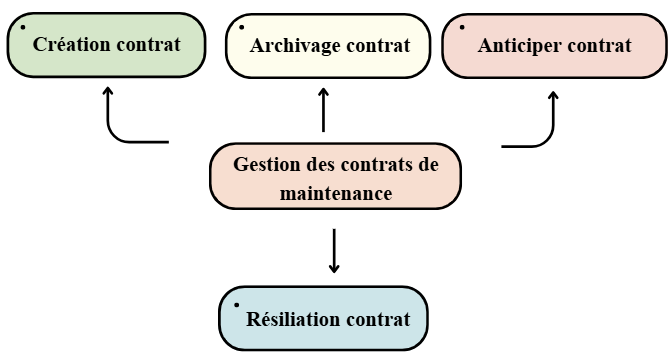
\includegraphics[width=0.7\textwidth,keepaspectratio]{Images/gestion_contrat.png}
    \caption{Gestion des contrats de maintenance}
    \label{fig:gestion_contrats}
\end{figure}

\subsubsection{Gestion des Demandes d'Intervention}

Ce module structure la soumission des demandes d'intervention avec vérification automatique de couverture contractuelle et validation des types d'intervention éligibles. Le processus de validation intègre un système de relance automatique garantissant le traitement dans les délais impartis avec escalade vers les responsables en cas de dépassement des seuils temporels.

\begin{figure}[H]
    \centering
    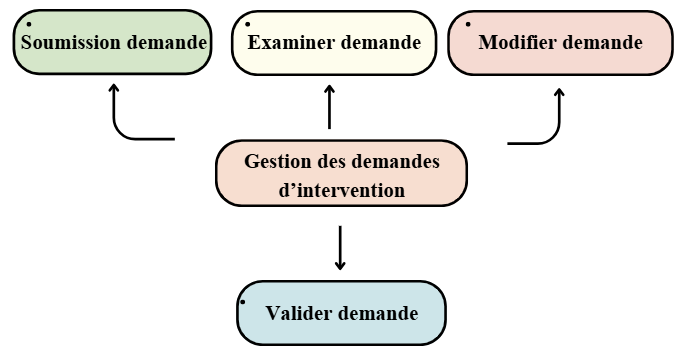
\includegraphics[width=0.7\textwidth,keepaspectratio]{Images/gestion_demande.png}
    \caption{Gestion des demandes d'intervention}
    \label{fig:gestion_demandes}
\end{figure}

\subsubsection{Gestion Avancée des Tickets de Maintenance}

Ce module recommande automatiquement les développeurs les plus adaptés à un ticket, permet de suivre le temps de travail via chronométrage, et de signaler des blocages avec analyse automatique par IA. Les solutions sont proposées collaborativement entre membres de l'équipe. La soumission en revue déclenche la clôture automatique des sessions et le calcul du temps cumulé. Après validation par le chef de projet, le client peut fermer le ticket, signaler un problème persistant, ou obtenir une extension automatique de sept jours.
\subsubsection{Tableaux de Bord, Traçabilité et Documentation}

Ce module offre des tableaux de bord personnalisés par rôle avec indicateurs clés de performance. Il maintient un historique exhaustif de toutes les opérations avec traçabilité complète et système de notifications multicanaux (web, email, Slack). La génération automatique de procès-verbaux PDF s'effectue à partir des informations de tickets lors de la résolution, produisant une documentation contractuelle structurée.

\begin{figure}[H]
    \centering
    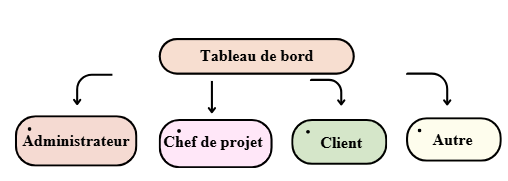
\includegraphics[width=0.7\textwidth,keepaspectratio]{Images/dashboard.png}
    \caption{Tableau de bord et reportage}
    \label{fig:dashboard}
\end{figure}

\begin{figure}[H]
    \centering
    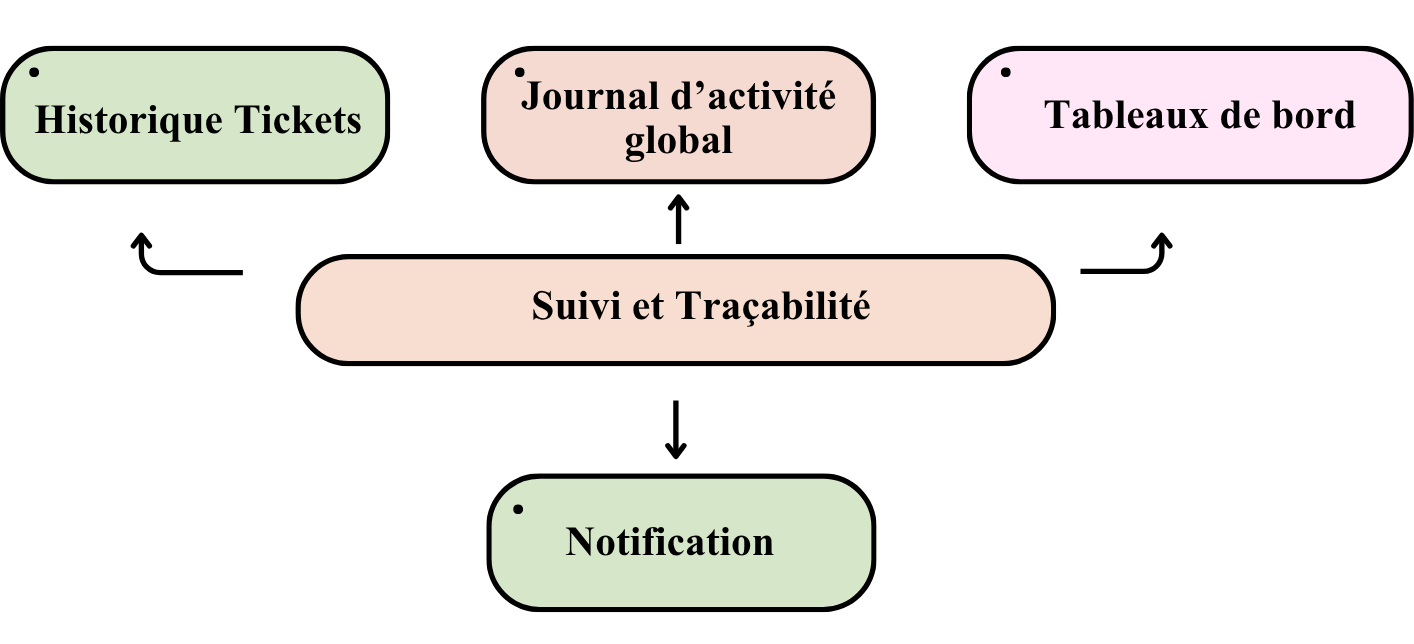
\includegraphics[width=0.7\textwidth,keepaspectratio]{Images/suivi_tracabilite.png}
    \caption{Suivi et Traçabilité}
    \label{fig:suivi_tracabilite}
\end{figure}

\begin{figure}[H]
    \centering
    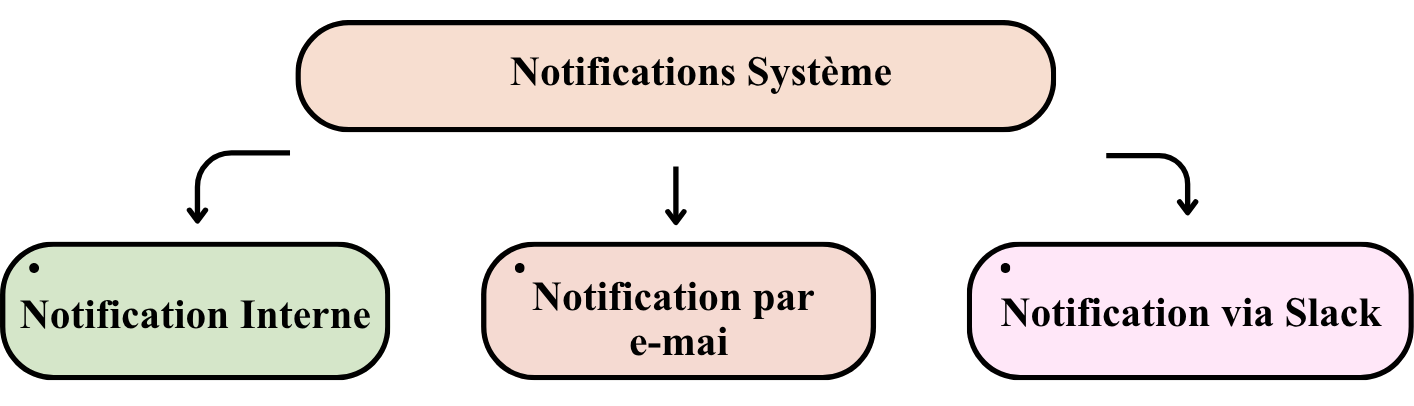
\includegraphics[width=0.7\textwidth,keepaspectratio]{Images/notifications.png}
    \caption{Notifications Système}
    \label{fig:notifications}
\end{figure}

\subsection{Identification des besoins non fonctionnels}
Afin de garantir la qualité logicielle, la robustesse et la pérennité de la plateforme, plusieurs exigences non fonctionnelles ont été définies et prises en compte lors de la conception et du développement :

\begin{itemize}[label=$\blacktriangleright$]

\item \textbf{Ergonomie et Accessibilité :} 
L'interface utilisateur doit offrir une utilisabilité optimale, caractérisée par une navigation fluide, une cohérence visuelle et une architecture adaptative (\textit{responsive design}). La plateforme doit intégrer des mécanismes de confort visuel, notamment à travers un système de thématisation dynamique (modes clair et sombre), et supporter nativement l'internationalisation pour garantir une accessibilité multilingue.

\item \textbf{Sécurité :} 
Le système doit assurer une protection rigoureuse de l'application et des données à travers des mécanismes d'authentification forte, une gestion stricte des autorisations basée sur les rôles (RBAC), et le chiffrement des informations sensibles. La traçabilité des actions critiques doit être garantie par un système de journalisation (\textit{logging}) permanent afin de permettre l'audit des événements et de détecter toute anomalie ou tentative d'accès non autorisé.

\item \textbf{Performance et Évolutivité :} 
Afin de garantir des latences minimales, même sous affluence critique, l'architecture doit intégrer des stratégies d'optimisation de l'accès aux données (mise en cache, requêtes optimisées) prenant en compte la sollicitation liée à l'opération d'indexation, tout en supportant une montée en charge progressive.

\item \textbf{Réactivité et Temps Réel :} 
Pour les modules nécessitant une synchronisation instantanée (tels que les notifications ou les alertes de gestion), le système doit garantir une communication bidirectionnelle à faible latence entre le serveur et les clients afin d'assurer la transmission immédiate des flux d'informations.

\item \textbf{Maintenabilité et Extensibilité :} 
Le code source doit être structuré de manière modulaire en respectant les standards de conception logicielle (notamment les principes SOLID). Cela assure une maintenance facilitée, une documentation claire des interfaces (API) et une couverture de tests automatisés pour prévenir les régressions lors des évolutions futures.

\end{itemize}

%─────────────────────────────────────────────────────────────────────────────
% SECTION II : MODÉLISATION DES BESOINS
%─────────────────────────────────────────────────────────────────────────────

\section{Modélisation des besoins}
\label{sec:modelisation_besoins}
L'analyse des besoins fonctionnels se poursuit par une modélisation dynamique à
l'aide du diagramme de cas d'utilisation UML. Ce diagramme offre une vision
synthétique des fonctionnalités offertes par le système du point de vue de chaque
acteur, sans se préoccuper de leur ordre d'exécution ou des détails techniques.

La figure \ref{fig:use_case} présente le diagramme de cas d'utilisation global de
notre plateforme de service desk. Ce diagramme structure les interactions entre les
six acteurs identifiés et le système. Chaque acteur possède un périmètre d'actions
bien défini.

\begin{figure}[H]
\centering
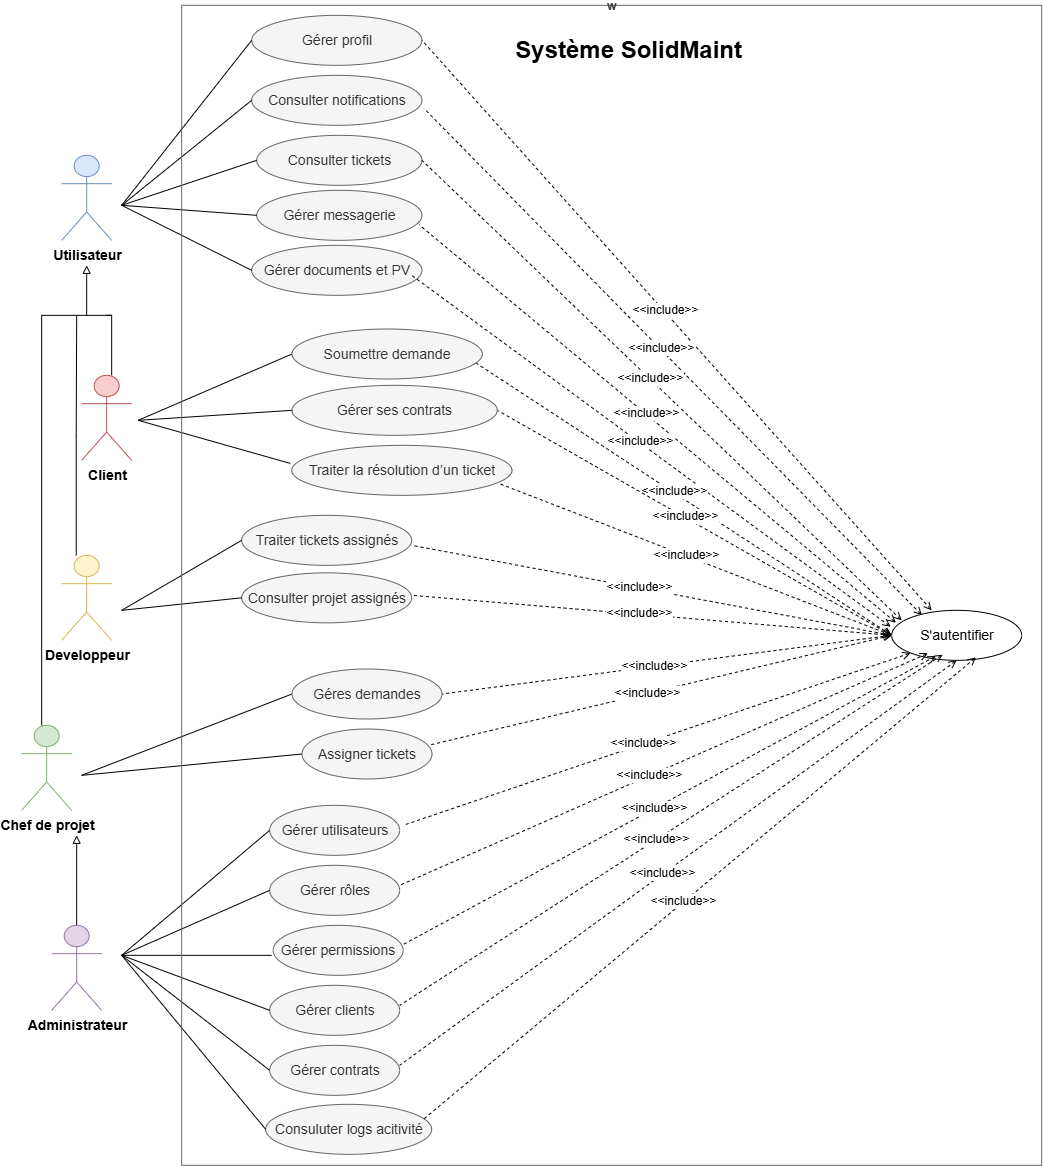
\includegraphics[width=1.0\textwidth,height=0.85\textheight,keepaspectratio]
  {Images/diagramme_cas_utilisation.png}
\caption{Diagramme de cas d'utilisation global du système}
\label{fig:use_case}
\end{figure}

%─────────────────────────────────────────────────────────────────────────────
% SECTION III : PILOTAGE AVEC SCRUM
%─────────────────────────────────────────────────────────────────────────────

\section{Pilotage du projet avec Scrum}
\label{sec:pilotage_scrum}

\subsection{Rôles de SCRUM}
Dans notre projet, Monsieur Mejdi Dhokar sera le Product Owner, Madame Maissa Ben
Fredj sera le Scrum Master, et nous, Rihab Chourou et Eya Gharbi, formons l'équipe
de développement.

\begin{figure}[H]
\centering
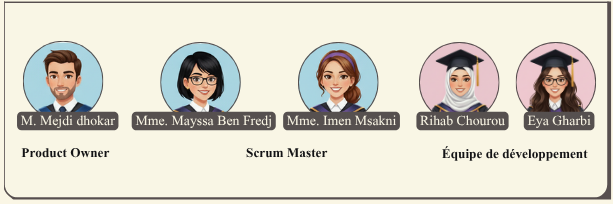
\includegraphics[width=0.9\textwidth,keepaspectratio]{Images/Equipe_Scrum.png}
\caption{Équipe Scrum et rôles}
\end{figure}

\subsubsection{Backlog de produit}
Comme évoqué dans le premier chapitre, le Product Backlog constitue l'un des
artefacts fondamentaux de la méthodologie Scrum. Il permet de formaliser les
exigences fonctionnelles ainsi que les fonctionnalités attendues du système. Le
tableau ci-dessous présente le Product Backlog de notre solution \textbf{SolidMaint},
structuré selon les éléments suivants :

\begin{itemize}[nosep,leftmargin=1.6cm,topsep=0pt,itemsep=2pt,label=$\bullet$]
  \item \textbf{Id EPIC} : Identifiant unique attribué à chaque EPIC afin de
    faciliter son identification et sa gestion dans le système de projet.
  \item \textbf{EPIC} : Ensemble de tâches interconnectées visant à atteindre un
    objectif majeur dans la gestion agile de projet ou le développement logiciel.
  \item \textbf{Id User Story} : Valeur unique et incrémentale associée à chaque
    user story pour assurer sa traçabilité.
  \item \textbf{User Story} : Description de la fonctionnalité du point de vue de
    l'utilisateur final, suivant le format ``En tant que [rôle], je souhaite [action]
    afin de [bénéfice]''.
  \item \textbf{Critères d'acceptation} : Conditions spécifiques et mesurables qui
    doivent être remplies pour que la user story soit considérée comme terminée et
    acceptée par le Product Owner.
  \item \textbf{Priorité} : Niveau d'importance défini par le Product Owner pour
    chaque tâche, permettant de prioriser les développements.
\end{itemize}

\noindent\textbf{Légende des priorités :} + : Faible \quad ++ : Moyenne \quad
+++ : Élevée.

\rowcolors{0}{}{}
\arrayrulecolor{black}
\renewcommand{\arraystretch}{1.2}
\small

% Au début de la longtable, remplace l'en-tête par :
\begin{longtable}{|C{1cm}|C{2.8cm}|M{1.2cm}|>{\raggedright\arraybackslash}p{4.7cm}|>{\raggedright\arraybackslash}p{4.5cm}|M{1.3cm}|}

   
    \rowcolor{lightblue}
    \textbf{ID Epic} & \textbf{Épic} & \textbf{ID US} & \multicolumn{1}{c|}{\textbf{User Story}} & \multicolumn{1}{c|}{\textbf{Critères d'acceptation}} & \textbf{Priorité} \\
    \hline
    \endfirsthead

    \hline
    \endhead

\hline
\endfoot

\hline
\endlastfoot

% Epic 1: Authentification et Sécurité
\multirow{5}{*}{\centering 1} & \multirow{5}{2.5cm}{\centering Authentification et Sécurité} 
& US01 & En tant qu'\textbf{utilisateur}, je souhaite m'authentifier avec email et mot de passe afin d'accéder à mes informations de manière sécurisée. 
& L'utilisateur authentifié avec succès accède à son tableau de bord personnalisé selon son rôle. & +++ \\
\cline{3-6}
& & US02 & En tant qu'\textbf{utilisateur}, je souhaite réinitialiser mon mot de passe afin de retrouver l'accès à mon compte. 
& L'utilisateur reçoit un email avec un lien valide 24h et peut définir un nouveau mot de passe conforme aux règles de sécurité. & +++ \\
\cline{3-6}
& & US03 & En tant qu'\textbf{utilisateur}, je souhaite m'authentifier via Google ou GitHub afin de me connecter rapidement sans créer de compte. 
& L'utilisateur peut se connecter via son compte Google ou GitHub et accéder immédiatement à l'application. & ++ \\
\cline{3-6}
& & US04 & En tant qu'\textbf{utilisateur}, je souhaite me déconnecter de la plateforme afin de sécuriser ma session. 
& Après déconnexion, l'utilisateur ne peut plus accéder aux pages protégées sans se reconnecter. & ++ \\
\cline{3-6}
& & US05 & En tant qu'\textbf{utilisateur}, je souhaite que mon compte soit protégé contre les tentatives de connexion malveillantes afin de garantir la sécurité de mes données. 
& Après 3 tentatives échouées, le compte est temporairement verrouillé et l'utilisateur reçoit une notification par email. & +++ \\
\hline

\multirow{2}{*}{\centering 2} & \multirow{5}{2.5cm}{\centering Gestion des utilisateurs } 

% Epic 2: Gestion des utilisateurs 

& US06 & En tant qu'\textbf{utilisateur}, je souhaite gérer mon profil afin que mes informations soient toujours à jour. 
& L'utilisateur peut modifier et sauvegarder ses informations personnelles qui sont validées avant enregistrement. & ++ \\
\cline{3-6}
& & US07 & En tant qu'\textbf{utilisateur}, je souhaite consulter l'historique de mes activités afin de suivre mes actions dans le système. 
& L'utilisateur visualise toutes ses actions passées avec possibilité de filtrer par date et type d'action. & ++ \\

\cline{3-6}
& & US08 & En tant qu'\textbf{administrateur}, je souhaite créer des utilisateurs afin de gérer les accès au système. 
& Le nouvel utilisateur reçoit un email d'invitation avec un mot de passe temporaire pour sa première connexion. & +++ \\
\cline{3-6}
& & US09 & En tant qu'\textbf{administrateur}, je souhaite modifier les informations d'un utilisateur afin de maintenir des données à jour. 
& Les modifications sont enregistrées avec traçabilité et l'utilisateur concerné est notifié des changements. & ++ \\
\cline{3-6}
& & US10 & En tant qu'\textbf{administrateur}, je souhaite activer et désactiver un compte utilisateur afin de contrôler l'accès au système. 
& Un compte désactivé ne peut plus se connecter et l'utilisateur reçoit une notification du changement de statut. & +++ \\
\cline{3-6}
& & US11 & En tant qu'\textbf{administrateur}, je souhaite consulter la liste des utilisateurs afin de visualiser et gérer efficacement les comptes. 
& La liste complète des utilisateurs est affichée avec possibilité de filtrer, rechercher et exporter les données. & ++ \\
\hline

% Epic 3: Gestion des rôles et permissions 
\multirow{5}{*}{\centering 3} & \multirow{5}{2.5cm}{\centering Gestion des rôles et permissions} 
& US12 & En tant qu'\textbf{administrateur}, je souhaite gérer des rôles afin de structurer les accès au système. 
& L'administrateur peut créer, modifier et archiver des rôles avec vérification des utilisateurs associés. & +++ \\
\cline{3-6}
& & US13 & En tant qu'\textbf{administrateur}, je souhaite attribuer des permissions granulaires aux rôles afin de contrôler précisément les accès. 
& L'administrateur sélectionne les permissions par catégorie et visualise un aperçu avant validation. & +++ \\
\cline{3-6}
& & US14 & En tant qu'\textbf{administrateur}, je souhaite consulter la matrice rôles-permissions afin de visualiser rapidement les droits de chaque rôle. 
& La matrice affiche clairement tous les rôles et leurs permissions avec possibilité de filtrer et exporter. & ++ \\
\hline
\enlargethispage{2cm}
% Epic 4: Demandes d'inscription OAuth
\multirow{2}{*}{\centering 4} & \multirow{2}{2.5cm}{\centering Gestion des demandes d'inscription OAuth} 
& US15 & En tant qu'\textbf{utilisateur externe}, je souhaite demander l'accès via OAuth afin de m'inscrire facilement. 
& La demande est enregistrée et l'administrateur reçoit une notification pour traitement. & ++ \\
\cline{3-6}
& & US16 & En tant qu'\textbf{administrateur}, je souhaite valider ou rejeter les demandes d'inscription OAuth afin de contrôler les accès. 
& L'utilisateur reçoit un email de confirmation ou rejet et peut accéder à l'application si validé. & +++ \\
\hline

% Epic 5: Gestion des clients et projets
\multirow{7}{*}{\centering 5} & \multirow{7}{2.5cm}{\centering Gestion des Clients et projets} 
& US17 & En tant qu'\textbf{administrateur}, je souhaite créer un profil client afin de centraliser ses informations. 
& Le profil client est créé avec toutes les informations nécessaires et un identifiant unique est généré. & +++ \\
\cline{3-6}
& & US18 & En tant qu’administrateur, je souhaite consulter la liste des clients  afin de visualiser les clients existants. 
& La liste complète des clients est accessible avec possibilité de filtrer, rechercher et exporter. & ++ \\
\cline{3-6}
& & US19 & En tant qu'\textbf{administrateur}, je souhaite consulter le profil détaillé d'un client afin de visualiser toutes ses informations. 
& Toutes les informations du client sont affichées incluant contrats, projets et historique des interactions. & ++ \\
\cline{3-6}
& & US20 & En tant qu'\textbf{administrateur}, je souhaite modifier les informations d'un client afin de maintenir des données à jour. 
& Les modifications sont enregistrées avec traçabilité et le client est notifié si ses coordonnées changent. & ++ \\
\cline{3-6}
& & US21 & En tant qu'\textbf{administrateur}, je souhaite activer et désactiver un compte client afin de contrôler l'accès. 
& Un compte client désactivé ne peut plus accéder au système et reçoit une notification du changement. & +++ \\
\cline{3-6}
& & US22 & En tant qu'\textbf{administrateur}, je souhaite imprimer l'annuaire d'un client afin de disposer d'une version papier. 
& Un document PDF professionnel contenant toutes les informations du client est généré. & + \\

\cline{3-6}
& &US23 & En tant qu'\textbf{administrateur}, je souhaite créer un projet rattaché à un client afin d'organiser les interventions. 
& Le projet est créé et rattaché au client avec un chef de projet assigné. & +++ \\
\cline{3-6}
& & US24 & En tant qu'\textbf{administrateur}, je souhaite consulter la liste des projets afin de piloter l'activité. 
& La liste complète des projets est affichée avec possibilité de filtrer par client, statut ou chef de projet. & ++ \\
\cline{3-6}
& & US25 & En tant qu'\textbf{administrateur}, je souhaite affecter des développeurs à un projet afin de constituer l'équipe. 
& Les développeurs sont affectés au projet et peuvent visualiser les informations du projet. & +++ \\
\cline{3-6}
& & US26 & En tant que \textbf{Développeur}, je souhaite consulter les informations du projet afin de comprendre le contexte. 
& Toutes les informations du projet sont accessibles incluant client, objectifs, équipe et contrat. & ++ \\
\hline
% Epic 6: Gestion des contrats
\multirow{7}{*}{\centering 6} & \multirow{7}{2.5cm}{\centering Gestion des Contrats} 

 & US27 & En tant qu'\textbf{administrateur}, je souhaite créer un contrat de maintenance afin de formaliser les engagements de service avec le client. 
& Le contrat est créé avec client, dates, type SLA, cycle facturation et configuration des alertes d'expiration. & +++ \\
\cline{3-6}
& & US28 & En tant qu'\textbf{administrateur}, je souhaite consulter la liste des contrats afin de suivre les engagements contractuels.
& La liste affiche tous les contrats avec filtres, indicateurs visuels d'expiration et possibilité d'export. & ++ \\
\cline{3-6}
& & US29 & En tant qu'\textbf{administrateur}, je souhaite recevoir des alertes avant l'expiration des contrats afin d'anticiper les renouvellements. 
& Des alertes automatiques sont envoyées à J-30, J-15 et J-7 par email, in-app et Slack. & +++ \\
\cline{3-6}
& & US30 & En tant qu'\textbf{administrateur}, je souhaite archiver un contrat afin de conserver l'historique. 
& Le contrat est archivé avec un changement de statut, avec possibilité de restauration ultérieure. & ++ \\
\cline{3-6}
& & US31 & En tant que \textbf{client}, je souhaite demander la résiliation de mon contrat afin d'interrompre le service. 
& La demande de résiliation est créée avec motif et date souhaitée, l'administrateur reçoit une notification et peut traiter la demande. & +++ \\
\cline{3-6}
& & US32 & En tant qu'\textbf{administrateur}, je souhaite résilier un contrat afin de l'interrompre avant terme. 
& Le contrat est résilié avec date et motif, les tickets ouverts sont clôturés et le client est notifié. & +++ \\
\cline{3-6}
& & US33 & En tant que \textbf{chef de projet}, je souhaite consulter les contrats dans un calendrier afin de visualiser les dates d'expiration.
& Le calendrier affiche les contrats avec leur date d'expiration. Les contrats proches de l'expiration sont mis en évidence. L'administrateur peut exporter le calendrier. & ++ \\
\cline{3-6}
& & US34 & En tant que \textbf{client}, je souhaite soumettre un retour d'expérience à l'expiration de mon contrat afin d'exprimer ma satisfaction.
& Le retour d’expérience est accessible pour les contrats expirés ou proches de l’expiration. Un seul retour d’expérience par contrat est accepté. & ++\\
\cline{3-6}
& & US35 & En tant qu'\textbf{administrateur}, je souhaite générer un PDF formaté du contrat afin de le partager avec le client.
& Le PDF généré contient les informations necessaires; les dates d'intervention& +\\
\cline{3-6}
& & US36 & En tant qu'\textbf{administrateur}, je souhaite consulter les détails d'un contrat afin de visualiser toutes ses informations.
& Toutes les informations du contrat sont affichées incluant client, dates, SLA, documents et historique. & ++ \\
\cline{3-6}
& & US37 & En tant qu'\textbf{équipe produit}, je souhaite réserver cet identifiant afin de conserver une numérotation continue du backlog.
& Identifiant réservé pour maintien de la cohérence de numérotation. & + \\
\hline

\multirow{8}{*}{\centering 8} & \multirow{8}{2.5cm}{\centering Gestion des demandes clients} 

% Epic 8: Gestion des demandes clients

& US38 & En tant que \textbf{client}, je souhaite soumettre une demande de maintenance afin de signaler un besoin. 
& Le client peut joindre des fichiers à sa demande. Le système génère un numéro unique de suivi. Le client reçoit une confirmation de réception. & +++ \\
\cline{3-6}
& & US39 & En tant que \textbf{chef de projet}, je souhaite consulter les demandes en attente afin de les traiter. 
& Le chef de projet visualise toutes les demandes nécessitant un traitement. Les demandes sont triées par date de création. Les demandes urgentes sont identifiables visuellement. & +++ \\
\cline{3-6}
& & US40 & En tant que \textbf{chef de projet}, je souhaite valider une demande afin de la convertir en ticket. 
& Le chef de projet peut approuver une demande. Le chef de projet définit la catégorie et la priorité. Un ticket est automatiquement créé et lié à la demande. & +++ \\
\cline{3-6}
& & US41 & En tant que \textbf{chef de projet}, je souhaite demander des informations complémentaires afin de clarifier une demande. 
& Le chef de projet peut solliciter des précisions au client. Le client est notifié de la demande d'informations. Un rappel est envoyé si aucune réponse après 48h. & ++ \\
\cline{3-6}
& & US42 & En tant que \textbf{client}, je souhaite compléter ma demande afin de fournir les informations manquantes. 
& Le client peut répondre aux questions posées. Le chef de projet est notifié de la réponse. La demande redevient disponible pour traitement. & ++ \\
\cline{3-6}
& & US43 & En tant que \textbf{chef de projet}, je souhaite requalifier une demande afin de corriger sa catégorie ou sa priorité. 
& Le chef de projet peut modifier la catégorie d'une demande. Le chef de projet peut ajuster la priorité. Une justification est obligatoire pour toute modification. Toutes les modifications sont tracées. & ++ \\
\cline{3-6}
& & US44 & En tant qu'\textbf{utilisateur}, je souhaite commenter une demande afin de communiquer sur le contexte. 
& L'utilisateur peut ajouter des commentaires à une demande. L'utilisateur peut joindre des fichiers aux commentaires. Les autres parties prenantes sont notifiées des nouveaux commentaires. & ++ \\
\cline{3-6}
& & US45 & En tant qu'\textbf{utilisateur}, je souhaite consulter l'historique d'une demande afin de suivre son évolution. 
& L'utilisateur visualise tous les événements liés à la demande. L'historique affiche la date et l'auteur de chaque action. L'utilisateur peut filtrer l'historique par type d'événement. & ++ \\
\hline
\multirow{20}{*}{\centering 9} & \multirow{20}{2.5cm}{\centering Gestion des tickets} 

% Epic 9: Gestion des tickets
 
& US46 & En tant que \textbf{développeur}, je souhaite visualiser mes tickets dans un tableau Kanban afin de gérer mes tâches. 
& Le développeur visualise ses tickets organisés par état d'avancement. Le développeur peut déplacer un ticket d'un état à un autre. Le développeur voit si un ticket risque de dépasser son délai. & +++ \\
\cline{3-6}
& & US47 & En tant que \textbf{chef de projet}, je souhaite assigner un ticket à un développeur afin de répartir la charge. 
& Le chef de projet sélectionne un développeur disponible. Le système alerte si le développeur a déjà trop de tickets. Le développeur assigné est notifié immédiatement. & +++ \\
\cline{3-6}
& & US48 & En tant que \textbf{chef de projet}, je souhaite assigner un ticket à plusieurs développeurs afin de collaborer sur des tâches complexes. 
& Le chef de projet peut assigner plusieurs développeurs au même ticket. Le chef de projet définit le rôle de chaque développeur. Le temps estimé est réparti entre les développeurs. & ++ \\
\cline{3-6}
& & US49 & En tant que \textbf{développeur}, je souhaite me désassigner d'un ticket afin de libérer ma charge. 
& Le développeur doit fournir un motif pour se désassigner. Le ticket redevient disponible pour assignation. Le chef de projet est notifié de la désassignation. & ++ \\
\cline{3-6}
& & US50 & En tant que \textbf{développeur}, je souhaite démarrer un chronomètre sur un ticket afin de tracker mon temps. 
& Le développeur peut démarrer le suivi du temps de travail. Une session de travail est créée avec l'heure de début. Le développeur voit le temps écoulé en temps réel. & +++ \\
\cline{3-6}
& & US51 & En tant que \textbf{développeur}, je souhaite mettre en pause mon chronomètre afin de gérer les interruptions. 
& Le développeur peut suspendre temporairement le suivi du temps. Le temps écoulé est enregistré. Le développeur peut reprendre le suivi ultérieurement. & ++ \\
\cline{3-6}
& & US52 & En tant que \textbf{développeur}, je souhaite arrêter le chronomètre afin de finaliser ma session. 
& Le développeur peut arrêter le suivi du temps. Le développeur peut ajouter un commentaire sur le travail effectué. La session est ajoutée à l'historique. Le développeur est alerté si le temps dépasse l'estimation. & +++ \\
\cline{3-6}
& & US53 & En tant que \textbf{développeur}, je souhaite ajouter manuellement une session de travail afin de corriger des oublis. 
& Le développeur peut enregistrer une session de travail passée. Le développeur doit fournir la date, l'heure et la durée. Le développeur doit justifier l'ajout manuel. Le système vérifie qu'il n'y a pas de chevauchement avec d'autres sessions. & ++ \\
\cline{3-6}
& & US54 & En tant que \textbf{développeur}, je souhaite changer le statut d'un ticket afin de refléter l'avancement. 
& Le développeur peut faire progresser un ticket selon le workflow défini. Le système empêche les transitions invalides. Toutes les parties prenantes sont notifiées lors d'un changement. L'historique des changements est conservé. & +++ \\
\cline{3-6}
& & US55 & En tant que \textbf{client}, je souhaite valider la résolution d'un ticket afin de confirmer que le problème est résolu. 
& Le client peut confirmer que le problème est résolu. Le client peut ajouter un commentaire de validation. Le ticket est fermé après validation. Le développeur est notifié de la validation. & +++ \\
\cline{3-6}
& & US56 & En tant que \textbf{chef de projet}, je souhaite rouvrir un ticket fermé afin de traiter un problème récurrent. 
& Le chef de projet doit justifier la réouverture. Le délai SLA est réinitialisé. Les développeurs assignés sont notifiés. & ++ \\
\cline{3-6}
& & US57 & En tant que \textbf{chef de projet}, je souhaite consulter le temps passé par ticket afin d'analyser la productivité. 
& Le chef de projet visualise le temps total passé sur chaque ticket. Le chef de projet voit le détail par développeur. Les données sont présentées sous forme de graphiques. & ++ \\
\cline{3-6}
& & US58 & En tant que \textbf{développeur}, je souhaite signaler un blocage afin d'alerter sur un obstacle. 
& Le développeur peut signaler un obstacle bloquant. Le développeur précise le type et l'impact du blocage. Le chef de projet reçoit une notification urgente. Le délai SLA est suspendu pendant le blocage. & +++ \\
\cline{3-6}
& & US59 & En tant que \textbf{membre d'équipe}, je souhaite résoudre un blocage afin de permettre au développeur de reprendre son travail. 
& Le blocage est résolu avec commentaire obligatoire, le chrono SLA reprend et l'action est tracée. & ++ \\
\cline{3-6}
& & US60 & En tant que \textbf{développeur}, je souhaite demander une extension de délai SLA afin de disposer de plus de temps. 
& La demande d'extension est créée avec durée et justification pour validation par le chef de projet. & ++ \\
\cline{3-6}
& & US61 & En tant que \textbf{chef de projet}, je souhaite approuver ou rejeter les demandes d'extension SLA. 
& La liste des demandes en attente est affichée, l'approbation ou rejet avec commentaire met à jour automatiquement le SLA. & ++ \\
\cline{3-6}
& & US62 & En tant qu'\textbf{utilisateur}, je souhaite commenter un ticket avec mentions afin de communiquer efficacement. 
& Les commentaires sont ajoutés avec éditeur riche, autocomplétion @utilisateur et distinction internes/externes. & +++ \\
\cline{3-6}
& & US63 & En tant qu'\textbf{utilisateur}, je souhaite ajouter des pièces jointes aux tickets afin de fournir du contexte. 
& Les fichiers sont ajoutés par drag \& drop (images/PDF/logs, max 10MB) avec prévisualisation. & ++ \\
\cline{3-6}
& & US64 & En tant que \textbf{développeur}, je souhaite être informé lorsqu'un autre utilisateur modifie le même ticket. 
& Une notification temps réel via WebSocket affiche un toast et un indicateur "X est en train d'éditer". & ++ \\
\cline{3-6}
& & US65 & En tant qu'\textbf{utilisateur}, je souhaite consulter l'historique complet d'un ticket afin de comprendre son évolution. 
& La timeline chronologique inversée affiche tous les événements avec filtres par type et export PDF. & ++ \\
\hline

% Epic 13: Dashboards et rapports - Calendrier et planification

\multirow{4}{*}{\centering 13} & \multirow{4}{2.5cm}{\centering Calendrier et planification}  
& US66 & En tant qu'\textbf{utilisateur}, je souhaite visualiser les tickets et demandes de maintenance sur un calendrier mensuel afin d'avoir une vue globale des interventions 
& L'utilisateur peut naviguer entre les mois, distinguer les types d'événements (Tickets/Demandes) par couleur et voir les titres tronqués. & +++ \\
\cline{3-6}
& & US67 & En tant qu'\textbf{administrateur}, je souhaite identifier visuellement les urgences SLA sur le calendrier afin de prioriser les interventions critiques. 
& Les événements en retard ou proches de l'échéance apparaissent en rouge/orange avec un indicateur visuel (pulse) sur les urgences critiques. & +++ \\
\cline{3-6}
& & US68 & En tant que \textbf{Chef de Projet}, je souhaite accéder à une vue Gantt / Agenda afin d'analyser la charge de travail et la progression de chaque développeur. 
&La vue affiche la timeline des affectations, le pourcentage de progression des tickets et le taux de charge calculé en temps réel par développeur. & ++ \\
\cline{3-6}
& & US69 & En tant qu'\textbf{utilisateur}, je souhaite accéder aux détails d'un ticket directement depuis le calendrier afin de consulter ou modifier l'intervention rapidement. 
& Un clic sur un événement dans le calendrier ou le panneau latéral redirige l'utilisateur vers la page de détails correspondante. & ++ \\
\hline
% Epic 10: Messagerie et collaboration
\multirow{9}{*}{\centering 10} & \multirow{9}{2.5cm}{\centering Messagerie et collaboration} 

& US70 & En tant qu'\textbf{utilisateur}, je souhaite accéder à une messagerie intégrée afin de communiquer avec mon équipe. 
& L'utilisateur visualise les canaux de discussion disponibles. L'utilisateur voit le nombre de messages non lus. L'utilisateur identifie les membres présents. & ++ \\
\cline{3-6}
& & US71 & En tant qu'\textbf{utilisateur}, je souhaite envoyer des messages dans un channel afin de communiquer. 
& L'utilisateur peut rédiger et envoyer des messages. L'utilisateur peut joindre des fichiers. Les messages sont reçus instantanément par les autres membres. & +++ \\
\cline{3-6}
& & US72 & En tant qu'\textbf{utilisateur}, je souhaite répondre à un message afin de créer un fil de discussion. 
& L'utilisateur peut répondre à un message spécifique. Les réponses sont regroupées dans un fil dédié. Seuls les participants au fil reçoivent les notifications. & ++ \\
\cline{3-6}
& & US73 & En tant qu'\textbf{utilisateur}, je souhaite mentionner des collègues afin d'attirer leur attention. 
& L'utilisateur peut mentionner un collègue dans un message. Le collègue mentionné reçoit une notification. Le message mentionné est mis en évidence pour le destinataire. & +++ \\
\cline{3-6}
& & US74 & En tant qu'\textbf{utilisateur}, je souhaite éditer mes messages afin de corriger des erreurs. 
& L'utilisateur peut modifier un message récemment envoyé. Le message modifié est identifiable. L'historique des modifications est conservé. & + \\
\cline{3-6}
& & US75 & En tant qu'\textbf{utilisateur}, je souhaite supprimer mes messages afin de retirer du contenu inapproprié. 
& L'utilisateur peut supprimer ses propres messages. Une confirmation est demandée avant suppression. Le message supprimé reste visible pour l'audit. & + \\
\cline{3-6}
& & US76 & En tant qu'\textbf{utilisateur}, je souhaite épingler des messages importants afin de les retrouver facilement. 
& L'utilisateur autorisé peut épingler un message. Les messages épinglés sont facilement accessibles. L'utilisateur peut retirer l'épinglage. & ++ \\
\cline{3-6}
& & US77 & En tant que \textbf{chef de projet}, je souhaite voir qui est en ligne dans mon équipe afin de savoir qui je peux solliciter. 
& Le chef de projet visualise les membres actuellement connectés. Le chef de projet peut filtrer par équipe ou projet. Le chef de projet voit l'heure de dernière activité. & ++ \\
\cline{3-6}
& & US78 & En tant qu'\textbf{utilisateur}, je souhaite voir qui est en ligne afin de savoir qui est disponible. 
& L'utilisateur voit le statut de disponibilité des autres membres. L'utilisateur peut modifier son propre statut. Le statut est visible par tous les membres. & ++ \\
\hline

\multirow{14}{*}{\centering 11} & \multirow{14}{2.5cm}{\centering Gestion des documents} 

% Epic 11: Gestion des documents
  
& US79 & En tant qu'\textbf{utilisateur}, je souhaite uploader des documents afin de centraliser les fichiers. 
& L'utilisateur peut téléverser des documents. L'utilisateur peut associer un document à un contrat, projet ou ticket. L'utilisateur peut ajouter un titre, une description et des tags. & ++ \\
\cline{3-6}
& & US80 & En tant qu'\textbf{utilisateur}, je souhaite télécharger des documents afin de les consulter hors ligne. 
& L'utilisateur peut télécharger un document individuel. L'utilisateur peut télécharger plusieurs documents simultanément. Le système vérifie les permissions avant le téléchargement. La consultation est enregistrée pour traçabilité. & ++ \\
\cline{3-6}
& & US81 & En tant qu'\textbf{utilisateur}, je souhaite gérer les versions des documents afin d'assurer la traçabilité. 
& L'utilisateur peut téléverser une nouvelle version d'un document existant. Le système numérote automatiquement les versions. L'utilisateur doit fournir un commentaire pour chaque nouvelle version. & ++ \\
\cline{3-6}
& & US82 & En tant qu'\textbf{utilisateur}, je souhaite consulter l'historique des consultations afin de voir qui a accédé au document. 
& L'utilisateur visualise qui a consulté le document. L'utilisateur voit la date et l'heure de chaque consultation. & + \\
\cline{3-6}
& & US83 & En tant qu'\textbf{utilisateur}, je souhaite archiver des documents afin de nettoyer la vue active. 
& L'utilisateur peut archiver un document. Une confirmation est demandée avant archivage. Le document archivé peut être restauré ultérieurement. & + \\
\cline{3-6}
& & US84 & En tant que \textbf{chef de projet}, je souhaite générer automatiquement un PV à partir d'un ticket afin de documenter les interventions. 
& Le chef de projet peut générer un procès-verbal depuis un ticket. Le document contient toutes les informations du ticket et les actions réalisées. Le document peut être signé électroniquement. & +++ \\
\cline{3-6}
& & US85 & En tant que \textbf{client}, je souhaite télécharger les PV de mes tickets afin de conserver une trace des interventions. 
& Le client peut accéder aux procès-verbaux depuis ses tickets. Le client visualise l'historique de tous les PV générés. Le client reçoit une notification lors de la génération d'un nouveau PV. & ++ \\
\cline{3-6}
& & US86 & En tant qu'\textbf{développeur ou chef de projet}, je souhaite consulter la base de connaissances afin de trouver des solutions existantes. 
& L'utilisateur peut rechercher par mots-clés, catégorie ou tags. Les résultats affichent titre et extrait. Un clic ouvre l'article complet. & ++ \\
\cline{3-6}
& & US87 & En tant qu'\textbf{administrateur}, je souhaite créer des articles de la base de connaissances afin d'enrichir la documentation. 
& L'administrateur peut créer des articles. La création est tracée et horodatée. L'historique des versions est conservé. & ++ \\
\cline{3-6}
& & US88 & En tant qu'\textbf{utilisateur}, je souhaite créer une nouvelle version d'un document afin de maintenir l'historique. 
& L'utilisateur peut téléverser une nouvelle version d'un document. L'utilisateur doit fournir un commentaire pour la nouvelle version. Le système numérote automatiquement les versions. Toutes les versions précédentes sont conservées. & ++ \\
\cline{3-6}
& & US89&  En tant qu'\textbf{utilisateur}, je souhaite comparer deux versions d'un document afin de voir les différences. 
& L'utilisateur peut sélectionner deux versions à comparer. Les deux versions sont affichées côte à côte. Les modifications sont mises en évidence. & + \\
\cline{3-6}
& & US90 & En tant qu'\textbf{administrateur}, je souhaite voir qui a consulté un document afin de suivre sa diffusion. 
& L'administrateur visualise la liste des consultations du document. L'historique indique la date, l'heure et l'utilisateur. Des statistiques de consultation sont disponibles. & ++ \\
\hline

% Epic 12: Notifications
\multirow{5}{*}{\centering 12} & \multirow{5}{2.5cm}{\centering Notifications et alertes} 
& US91 & En tant qu'\textbf{utilisateur}, je souhaite recevoir des notifications in-app afin d'être informé en temps réel. 
& L'utilisateur visualise le nombre de notifications non lues. L'utilisateur peut consulter la liste des notifications. L'utilisateur peut marquer une notification comme lue. L'utilisateur peut accéder directement à l'élément concerné. & +++ \\
\cline{3-6}
& & US92 & En tant qu'\textbf{utilisateur}, je souhaite recevoir des notifications par email afin d'être informé hors connexion. 
& L'utilisateur peut configurer la fréquence des notifications email. L'utilisateur reçoit des emails pour les événements importants. & ++ \\
\cline{3-6}
& & US93 & En tant que \textbf{membre technique}, je souhaite recevoir des notifications Slack afin d'être alerté sur mon outil de travail. 
& L'administrateur peut configurer l'intégration Slack par contrat ou projet. Les événements importants sont envoyés sur Slack. & ++ \\
\cline{3-6}
& & US94 & En tant qu'\textbf{utilisateur}, je souhaite recevoir des notifications push navigateur afin d'être alerté même hors onglet. 
& L'utilisateur peut autoriser les notifications navigateur. L'utilisateur reçoit des alertes pour les événements critiques. L'utilisateur peut accéder à l'application en cliquant sur la notification. & ++ \\
\cline{3-6}
& & US95 & En tant qu'\textbf{utilisateur}, je souhaite consulter l'historique de mes notifications afin de retrouver une information. 
& L'utilisateur visualise toutes ses notifications passées. L'utilisateur peut filtrer par type ou période. L'utilisateur peut rechercher dans l'historique. & ++ \\
\hline

\multirow{8}{*}{\centering 13} & \multirow{8}{2.5cm}{\centering Dashboards et rapports } 

% Epic 13: Dashboards et rapports

& US96 & En tant qu'\textbf{administrateur}, je souhaite consulter un dashboard global afin de piloter le système. 
& L'administrateur visualise les indicateurs clés du système. L'administrateur peut filtrer les données par période. L'administrateur identifie les alertes nécessitant une action. & +++ \\
\cline{3-6}
& & US97 & En tant que \textbf{chef de projet}, je souhaite consulter un dashboard d'équipe afin de piloter l'activité. 
& Le chef de projet visualise la charge de travail de son équipe. Le chef de projet suit la performance par rapport aux délais. Le chef de projet compare le temps passé au temps estimé. & +++ \\
\cline{3-6}
& & US98 & En tant que \textbf{développeur}, je souhaite consulter mon dashboard personnel afin d'organiser ma journée. 
& Le développeur visualise ses tickets assignés. Le développeur voit ses priorités du jour. Le développeur suit son temps de travail. Le développeur identifie les échéances proches. & ++ \\
\cline{3-6}
& & US99 & En tant que \textbf{client}, je souhaite consulter mon dashboard afin de suivre mes projets. 
& Le client visualise ses contrats actifs. Le client suit l'état de ses demandes et tickets. Le client accède à ses documents récents. Le client identifie ses contacts dans l'équipe. & ++ \\
\cline{3-6}
& & US100 & En tant qu'\textbf{administrateur}, je souhaite générer un rapport d'activité mensuel afin de présenter les statistiques. 
& L'administrateur génère un rapport pour une période donnée. Le rapport contient les tickets traités et le temps passé. Le rapport indique le respect des délais. Le rapport peut être exporté. & +++ \\
\cline{3-6}
& & US101 & En tant qu'\textbf{administrateur}, je souhaite générer des rapports de conformité SLA afin de justifier les performances. 
& L'administrateur génère un rapport de conformité par contrat. Le rapport affiche le taux de respect des délais. Le rapport détaille les tickets en dépassement. & +++ \\
\cline{3-6}
& & US102 & En tant que \textbf{chef de projet}, je souhaite générer des rapports d'activité afin de présenter l'avancement. 
& Le chef de projet génère un rapport pour son équipe ou projet. Le rapport affiche les tickets traités et le temps passé. Le rapport présente l'évolution de l'activité. & ++ \\
\hline

% Epic 14: Historique et audit trail
\multirow{2}{*}{\centering 14} & \multirow{2}{2.5cm}{\centering Historique et traçabilité} 
& US103 & En tant qu'\textbf{administrateur}, je souhaite consulter l'historique complet de toutes les actions afin d'assurer la traçabilité. 
& L'administrateur visualise toutes les actions effectuées dans le système. L'historique indique l'utilisateur, la date et l'action réalisée. L'historique conserve les valeurs avant et après modification. & +++ \\
\cline{3-6}
& & US104 & En tant qu'\textbf{administrateur}, je souhaite exporter les logs d'audit afin de répondre aux exigences de conformité. 
& L'administrateur peut exporter l'historique des actions. L'administrateur peut filtrer par période, utilisateur ou type d'action. Les données exportées sont sécurisées. & ++ \\
\hline

% Epic 16: Assistance intelligente
\multirow{7}{*}{\centering 16} & \multirow{7}{2.5cm}{\centering Assistance intelligente} 
& US105 & En tant que \textbf{chef de projet}, je souhaite que l'IA analyse automatiquement les blocages afin d'identifier rapidement les problèmes critiques. 
& L'analyse est automatique lors du signalement. Le résultat est affiché dans l'interface. Un résumé clair du problème est présenté. & +++ \\
\cline{3-6}
& & US106 & En tant que \textbf{chef de projet}, je souhaite que l'IA propose des actions correctives afin de débloquer rapidement un développeur. 
& L'IA affiche 1 à 3 actions suggérées par blocage. Chaque action inclut destinataire et durée estimée. Le chef de projet peut valider une action qui crée automatiquement une tâche. & +++ \\
\cline{3-6}
& & US107 & En tant que \textbf{développeur}, je souhaite qu'un brouillon de solution soit généré à la fermeture d'un ticket afin de faciliter la documentation. 
& Un brouillon est créé automatiquement contenant : problème identifié, actions réalisées, résultat. Le développeur peut modifier le brouillon avant publication. & +++ \\
\cline{3-6}
& & US108 & En tant que \textbf{chef de projet}, je souhaite que l'IA propose une classification des demandes clients afin d'accélérer leur traitement, avec validation avant transmission au client. 
& L'IA propose type/priorité/catégorie. Le chef de projet peut accepter, modifier ou rejeter. La classification validée est visible par le client. L'audit trace proposition IA vs choix final. & +++ \\
\cline{3-6}
& & US110 & En tant que \textbf{chef de projet}, je souhaite que l'IA structure automatiquement les solutions saisies en articles KB afin d'améliorer la documentation. 
& La solution brute est transformée en format structuré (Problème/Solution/Détails). Des tags sont générés automatiquement. L'auteur peut modifier avant publication. & ++ \\
\cline{3-6}
& & US111 & En tant que \textbf{chef de projet}, je souhaite que l'IA fusionne le brouillon d'un blocage avec la solution humaine afin de produire un article KB définitif. 
& La fusion est proposée pour les blocages résolus. L'article final combine l'analyse IA et la solution humaine. Le responsable peut valider ou modifier avant publication. & + \\
\hline


 \caption{Product Backlog} \label{tab:product_backlog} \\
    \hline
\end{longtable}

\subsection{Planification des sprints}
Le projet a été mené selon la méthodologie Scrum, structuré en quatre sprints successifs s'étalant sur une période globale d'environ quatres mois. Cette approche itérative suit une logique architecturale rigoureuse : la mise en place des fondations sécuritaires, le développement de la gestion contractuelle, l'implémentation du cœur métier, et enfin l'intégration des modules collaboratifs et analytiques.

Chaque itération respecte le cycle Scrum, initié par une phase de planification (\textit{Sprint Planning}) et clôturé par les phases de revue (\textit{Sprint Review}) et de rétrospective (\textit{Sprint Retrospective}).

La figure suivante présente le déroulement chronologique de nos sprints.

\begin{figure}[H]
\centering
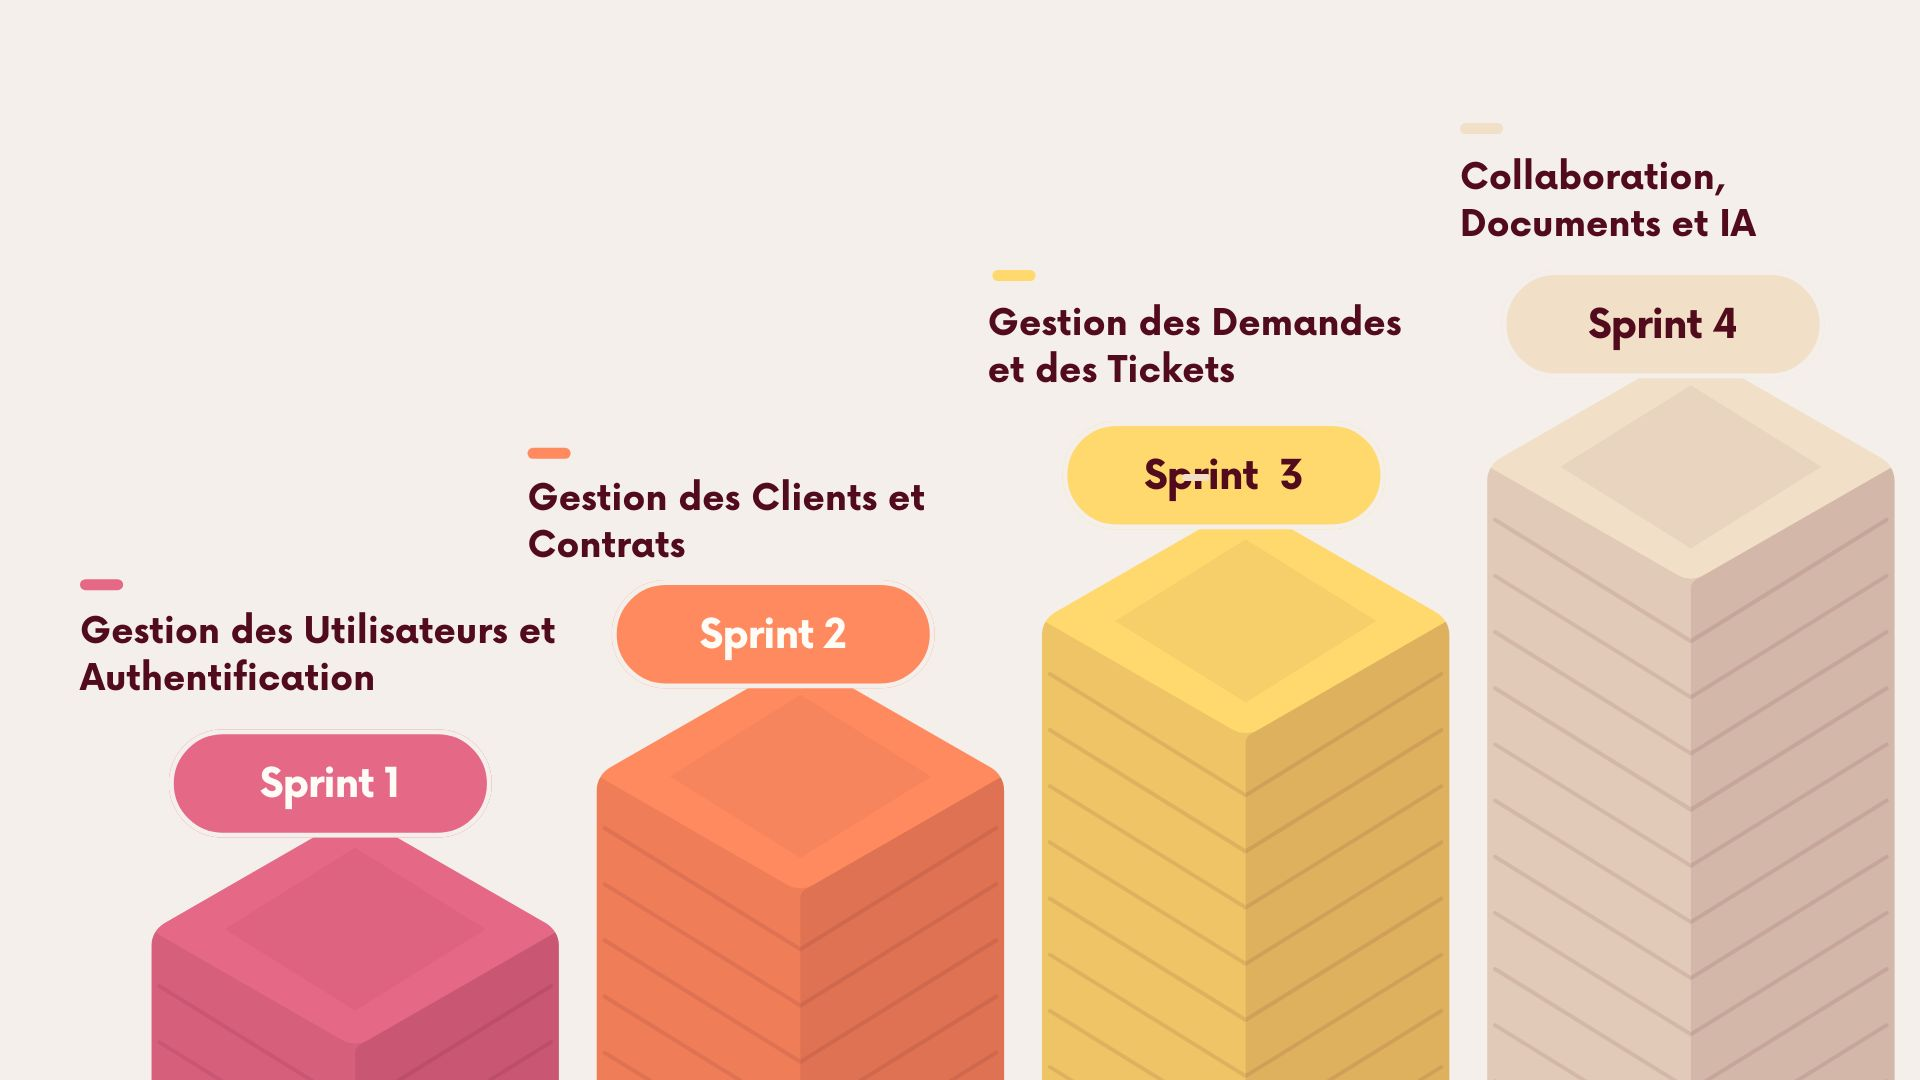
\includegraphics[width=0.8\textwidth,keepaspectratio]{Images/Scrum planning.jpg}
\caption{Planification chronologique des sprints}
\label{fig:planification_sprints}
\end{figure}

\subsubsection{Sprint 1 -- Authentification, Sécurité et Gestion des Utilisateurs}
\textbf{Période :} du 17 février au 11 mars (\textbf{3 semaines})
\newline
\textbf{Objectif du sprint :} Mettre en place le système d'authentification sécurisé
et la gestion complète des utilisateurs avec contrôle d'accès basé sur
les rôles (RBAC).

\noindent\textbf{User Stories sélectionnées :}
\begin{itemize}[nosep,leftmargin=1.6cm,topsep=0pt,itemsep=2pt,label=$\bullet$]
  \item \textbf{Epic 1 -- Authentification et Sécurité} : US01 à US05 (5 user stories)
  \item \textbf{Epic 2 -- Gestion des utilisateurs} : US06 à US11 (6 user stories)
  \item \textbf{Epic 3 -- Gestion des rôles et permissions} : US12 à US14 (3 user stories)
  \item \textbf{Epic 4 -- Demandes d'inscription OAuth} : US15 à US16 (2 user stories)
\end{itemize}

\noindent\textbf{Livrables attendus :}
\begin{itemize}[nosep,leftmargin=1.6cm,topsep=0pt,itemsep=2pt,label=$\bullet$]
  \item Système d'authentification fonctionnel (JWT + OAuth Google/GitHub)
  \item Module de gestion des utilisateurs avec verrouillage de compte
  \item Système RBAC complet avec gestion des rôles et permissions granulaires
\end{itemize}

\subsubsection{Sprint 2 -- Gestion des Clients, Projets et Contrats}
\textbf{Période :} du 12 mars au 2 avril (\textbf{3 semaines})
\newline
\textbf{Objectif du sprint :} Développer la gestion complète des clients, des projets et contrats
de maintenance avec système d'alertes d'expiration et configuration SLA.

\noindent
\textbf{User Stories sélectionnées :}
\begin{itemize}[nosep,leftmargin=1.6cm,topsep=0pt,itemsep=2pt,label=$\bullet$]
  \item \textbf{Epic 5 -- Gestion des clients et projets} : US17 à US26 (10 user stories)
  \item \textbf{Epic 6 -- Gestion des contrats} : US27 à US37 (10 user stories)
  \item \textbf{Epic 14 -- Historique et traçabilité} : US101 à US102 (2 user stories)
\end{itemize}

\noindent\textbf{Livrables attendus :}
\begin{itemize}[nosep,leftmargin=1.6cm,topsep=0pt,itemsep=2pt,label=$\bullet$]
  \item Module de gestion des clients avec profils société
  \item Module de gestion des projets avec équipes et membres
  \item Système de gestion des contrats avec SLA, alertes à J-30/J-15/J-7 et
    workflow d'approbation
  \item Système d'audit et traçabilité complet (ActivityLog)
\end{itemize}

\subsubsection{Sprint 3 -- Gestion des Demandes et Tickets}
\textbf{Période :} du 3 avril au 24 avril (\textbf{4 semaines})
\newline
\textbf{Objectif du sprint :} Implémenter le cœur métier avec la gestion des
demandes et tickets incluant suivi du temps, SLA et tableau Kanban.

\noindent\textbf{User Stories sélectionnées :}
\begin{itemize}[nosep,leftmargin=1.6cm,topsep=0pt,itemsep=2pt,label=$\bullet$]
  \item \textbf{Epic 7 -- Gestion des demandes} : US38 à US44 (7 user stories)
  \item \textbf{Epic 8 -- Gestion des tickets} : US45 à US64 (20 user stories)
  \item \textbf{Epic 15 -- Intelligence Artificielle} : US105 à US110 (6 user stories)
\end{itemize}

\noindent\textbf{Livrables attendus :}
\begin{itemize}[nosep,leftmargin=1.6cm,topsep=0pt,itemsep=2pt,label=$\bullet$]
  \item Module de gestion des demandes de maintenance avec classification
  \item Système complet de gestion des tickets avec vue Kanban (drag \& drop)
  \item Chronomètre de travail par session et respect des SLA en minutes ouvrées
  \item Moteur d'IA pour classification automatique des demandes et assistance intelligente
\end{itemize}

\subsubsection{Sprint 4 -- Collaboration, Documents et Planification}
\textbf{Période :} du 25 avril au 22 mai (\textbf{3 semaines})
\par\noindent\textbf{Objectif du sprint :} Finaliser les fonctionnalités avancées de
collaboration, de gestion documentaire, de notifications multicanales et de
planification.

\noindent\textbf{User Stories sélectionnées :}
\begin{itemize}[nosep,leftmargin=1.6cm,topsep=0pt,itemsep=2pt,label=$\bullet$]
  \item \textbf{Epic 9 -- Calendrier et planification} : US65 à US68 (4 user stories)
  \item \textbf{Epic 10 -- Messagerie et collaboration} : US69 à US77 (9 user stories)
  \item \textbf{Epic 11 -- Gestion des documents} : US78 à US88 (11 user stories)
  \item \textbf{Epic 12 -- Notifications et alertes} : US89 à US93 (5 user stories)
  \item \textbf{Epic 13 -- Dashboards et rapports} : US94 à US100 (7 user stories)
  \item \textbf{Epic 14 -- Historique et traçabilité} : US103 à US104 (2 user stories)
\end{itemize}

\noindent
\textbf{Livrables attendus :}
\begin{itemize}[nosep,leftmargin=1.6cm,topsep=0pt,itemsep=2pt,label=$\bullet$]
  \item Système de messagerie et collaboration temps réel (WebSocket)
  \item Module de gestion documentaire avec versioning et base de connaissances
  \item Système de notifications multicanaux (in-app, email, Slack et Web Push)
  \item Module de génération de rapports et procès-verbaux PDF
  \item Tableaux de bord pour pilotage et calendrier de planification
  \item Système de traçabilité et historique des activités
\end{itemize}

\noindent\textbf{Synthèse de la planification :} Cette répartition assure une
progression logique où chaque sprint s'appuie sur les livrables précédents. Les
dépendances techniques sont respectées (authentification avant tickets, contrats
avant demandes), et la valeur métier croît progressivement jusqu'aux fonctionnalités
différenciantes du sprint final.

\subsection{Planning prévisionnel (Diagramme de Gantt)}
\label{sec:planning}
« Un diagramme de Gantt est un outil d'organisation et de gestion de projets. Il
s'agit d'un diagramme à barres horizontales qui présente toutes les tâches d'un
projet en fonction d'un calendrier. Il aide les chefs de projet à visualiser les
tâches requises et à suivre l'avancement de leur projet. » [5]
\newline
Dans le cadre du développement de notre projet \textbf{SolidMaint}, le planning
prévisionnel a été réalisé pour organiser les différentes phases de développement.
La figure ci-dessous illustre cette planification :

\begin{figure}[H]
\centering
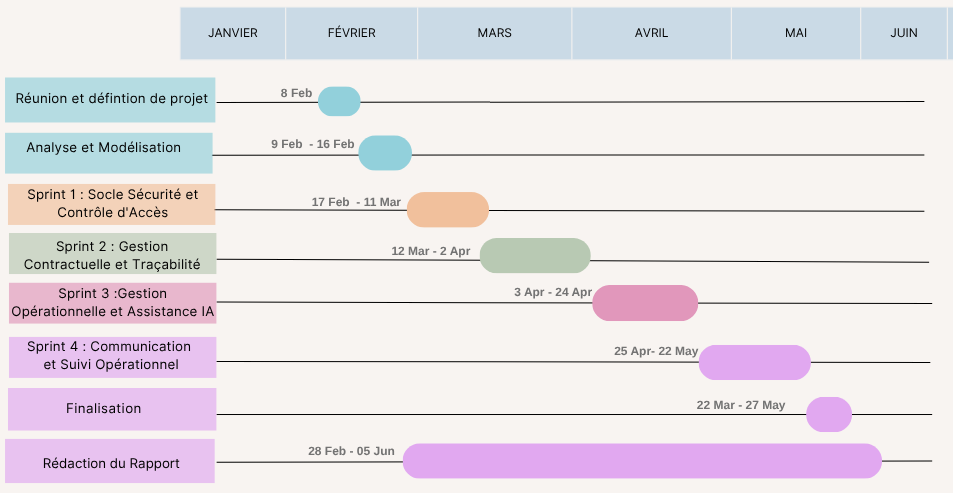
\includegraphics[width=0.7\textwidth,keepaspectratio]{Images/Diagramme_Gantt.png}
\caption{Diagramme de Gantt}
\end{figure}

%─────────────────────────────────────────────────────────────────────────────
% SECTION IV : ENVIRONNEMENT DE DÉVELOPPEMENT
%─────────────────────────────────────────────────────────────────────────────

\section{Environnement de Développement}
\label{sec:environnement}
On va commencer par la présentation de l'environnement matériel et logiciel que nous
utilisons.

\subsection{Environnement matériel}
\begin{table}[H]
\centering
\renewcommand{\arraystretch}{1.6}
\arrayrulecolor{gray!70}
\rowcolors{2}{gray!5}{white}
\begin{tabularx}{\textwidth}{| >{\centering\arraybackslash}X
                              | >{\centering\arraybackslash}X
                              | >{\centering\arraybackslash}X |}
\rowcolor{blue!20} \hline
\textbf{Ordinateur}        & \textbf{1}                          & \textbf{2}          \\
\hline
Propriétaire               & Rihab Chourou                       & Eya Gharbi          \\
\hline
Processeur                 & Core i3                             & Core i3             \\
\hline
RAM                        & 20 Go                               & 16 Go               \\
\hline
Disque dur                 & 1 To                                & 256 Go              \\
\hline
Système d'exploitation     & Windows 10 Professionnel N 64-bit   & Windows 10 Professionnel 64-bit \\
\hline
\end{tabularx}
\caption{Environnement matériel de développement}
\label{tab:environnement_de_developpement}
\end{table}

\subsection{Environnement logiciel}

\subsubsection{Langages de programmation et frameworks}
\vspace{12pt}

\newcommand{\cadretech}[2]{%
\noindent\begin{minipage}{1.8cm}\centering
  \includegraphics[width=1.5cm,keepaspectratio]{#1}
\end{minipage}\hspace{0.5cm}%
\begin{minipage}{\dimexpr\textwidth-1.8cm-0.5cm-2\fboxsep-2\fboxrule\relax}
  \fbox{\parbox{\dimexpr\linewidth-2\fboxsep\relax}{#2}}
\end{minipage}\par\vspace{10pt}}

\cadretech{Images/nestjs.png}{%
  \textbf{NestJS v11 :} « C'est un framework permettant de créer des applications
  serveur Node.js performantes et évolutives. Il utilise JavaScript progressif, est
  conçu avec TypeScript et le prend entièrement en charge (tout en permettant aux
  développeurs de coder en JavaScript pur). » [6]}

\cadretech{Images/nextjs.png}{%
  \textbf{Next.js v16 :} « C'est un framework React permettant de créer des
  applications web complètes. Il configure également automatiquement les outils de
  bas niveau tels que les modules de regroupement et les compilateurs. » [7]}

\cadretech{Images/React-icon.png}{%
  \textbf{React 18.3 :} « React est une bibliothèque JavaScript pour la construction
  d'interfaces utilisateur. Elle permet de créer des composants réutilisables qui
  gèrent leur propre état et se composent pour former des interfaces complexes. » [8]}

\cadretech{Images/Tailwind.png}{%
  \textbf{Tailwind CSS v4.2 :} « Un framework CSS utilitaire, doté de classes telles
  que \texttt{flex}, \texttt{pt-4}, \texttt{text-center} et \texttt{rotate-90}, qui
  peuvent être combinées pour créer n'importe quel design, directement dans votre
  balisage. » [9]}

\cadretech{Images/chadcn.png}{%
  \textbf{shadcn/ui v3.8 :} « est un ensemble de composants élégants et accessibles,
  ainsi qu'une plateforme de distribution de code. Compatible avec vos frameworks et
  modèles d'IA préférés. Logiciel libre. » [10]}

\subsubsection{Outils de développement et modélisation}
\vspace{12pt}

\newcommand{\cadretechVscode}[2]{%
\noindent\begin{minipage}{2.2cm}\centering
  \includegraphics[width=2cm,height=1.5cm,keepaspectratio]{#1}
\end{minipage}\hspace{0.5cm}%
\begin{minipage}{\dimexpr\textwidth-2.2cm-0.5cm-2\fboxsep-2\fboxrule\relax}
  \fbox{\parbox{\dimexpr\linewidth-2\fboxsep\relax}{#2}}
\end{minipage}\par\vspace{10pt}}

\cadretechVscode{Images/Visual_Studio_Code.png}{%
  \textbf{Visual Studio Code :} « est un éditeur de code source léger mais puissant,
  disponible sur Windows, macOS et Linux. Il intègre la coloration syntaxique, la
  complétion intelligente du code (IntelliSense), le débogage, le contrôle de version
  Git et une riche bibliothèque d'extensions. » [11]}

\newcommand{\cadretechGitlab}[2]{%
    \noindent
    \begin{minipage}{2.2cm}
        \centering
        \includegraphics[width=2cm, height=1.5cm, keepaspectratio]{#1}
    \end{minipage}
    \hspace{0.5cm}
    \begin{minipage}{\dimexpr\textwidth-2.2cm-0.5cm-2\fboxsep-2\fboxrule\relax}
        \fbox{%
            \parbox{\dimexpr\linewidth-2\fboxsep\relax}{%
                #2%
            }%
        }%
    \end{minipage}
    \par
    \vspace{10pt}
}
\cadretechGitlab{Images/gitlab.png}{ \textbf{GitLab : } « offre un espace de stockage de code en ligne ainsi que des fonctionnalités de suivi des problèmes et d'intégration continue/déploiement continu ( CI/CD). Le dépôt permet d'héberger différentes branches de développement et
  versions. » [12]}

\newcommand{\cadretechUml}[2]{%
\noindent\begin{minipage}{2.2cm}\centering
  \includegraphics[width=2cm,height=1.5cm,keepaspectratio]{#1}
\end{minipage}\hspace{0.5cm}%
\begin{minipage}{\dimexpr\textwidth-2.2cm-0.5cm-2\fboxsep-2\fboxrule\relax}
  \fbox{\parbox{\dimexpr\linewidth-2\fboxsep\relax}{#2}}
\end{minipage}\par\vspace{10pt}}

\cadretechUml{Images/uml.png}{%
  \textbf{UML :} « est un langage permettant de spécifier, visualiser, construire et
  documenter les artefacts des systèmes logiciels, ainsi que de modéliser des systèmes
  métier et d'autres systèmes non logiciels. L'UML représente un ensemble de bonnes
  pratiques d'ingénierie qui ont fait leurs preuves dans la modélisation de systèmes
  vastes et complexes. » [13]}

\newcommand{\cadretechDrowio}[2]{%
\noindent\begin{minipage}{2.2cm}\centering
  \includegraphics[width=2cm,height=1.5cm,keepaspectratio]{#1}
\end{minipage}\hspace{0.5cm}%
\begin{minipage}{\dimexpr\textwidth-2.2cm-0.5cm-2\fboxsep-2\fboxrule\relax}
  \fbox{\parbox{\dimexpr\linewidth-2\fboxsep\relax}{#2}}
\end{minipage}\par\vspace{10pt}}

\cadretechDrowio{Images/lucidchart.png}{%
  \textbf{Lucidchart :} « est un environnement de travail visuel qui associe création
  de diagrammes, visualisation de données et fonctionnalités de collaboration afin de
  faciliter la communication et stimuler l'innovation. » [14]}

\newcommand{\cadretechSwagger}[2]{%
\noindent\begin{minipage}{2.2cm}\centering
  \includegraphics[width=2cm,height=1.5cm,keepaspectratio]{#1}
\end{minipage}\hspace{0.5cm}%
\begin{minipage}{\dimexpr\textwidth-2.2cm-0.5cm-2\fboxsep-2\fboxrule\relax}
  \fbox{\parbox{\dimexpr\linewidth-2\fboxsep\relax}{#2}}
\end{minipage}\par\vspace{10pt}}

\cadretechSwagger{Images/swagger.png}{%
  \textbf{Swagger / OpenAPI :} « Swagger permet la conception, la gouvernance et les
  tests tout au long du cycle de vie complet des API, garantissant ainsi la qualité à
  chaque étape. Il génère automatiquement une documentation interactive de l'API à
  partir des annotations du code source. » [15]}

\subsubsection{Systèmes de gestion de bases de données}
\vspace{12pt}

\newcommand{\cadretechPrisma}[2]{%
\noindent\begin{minipage}{2.2cm}\centering
  \includegraphics[width=2cm,height=1.5cm,keepaspectratio]{#1}
\end{minipage}\hspace{0.5cm}%
\begin{minipage}{\dimexpr\textwidth-2.2cm-0.5cm-2\fboxsep-2\fboxrule\relax}
  \fbox{\parbox{\dimexpr\linewidth-2\fboxsep\relax}{#2}}
\end{minipage}\par\vspace{10pt}}

\cadretechPrisma{Images/prisma.png}{%
  \textbf{Prisma ORM v7 :} « est un ORM open source de nouvelle génération qui offre
  un accès rapide et sécurisé aux bases de données PostgreSQL, MySQL et autres. Il
  fournit un client typé généré automatiquement à partir du schéma de données,
  garantissant la sécurité des types à la compilation et des requêtes SQL optimisées
  à l'exécution. » [16]}

\newcommand{\cadretechPostgres}[2]{%
\noindent\begin{minipage}{2.2cm}\centering
  \includegraphics[width=2cm,height=1.5cm,keepaspectratio]{#1}
\end{minipage}\hspace{0.5cm}%
\begin{minipage}{\dimexpr\textwidth-2.2cm-0.5cm-2\fboxsep-2\fboxrule\relax}
  \fbox{\parbox{\dimexpr\linewidth-2\fboxsep\relax}{#2}}
\end{minipage}\par\vspace{10pt}}

\cadretechPostgres{Images/postgres.png}{%
  \textbf{PostgreSQL 16 :} « est un système de gestion de bases de données
  objet-relationnelles (SGBD-OR) open source. Il a été pionnier dans de nombreux
  concepts qui ne sont devenus disponibles que bien plus tard dans certains systèmes
  de bases de données commerciaux. Il est reconnu pour sa robustesse, sa conformité
  aux standards SQL et ses performances sur de grands volumes de données. » [17]}

\newcommand{\cadretechRedis}[2]{%
\noindent\begin{minipage}{2.2cm}\centering
  \includegraphics[width=2cm,height=1.5cm,keepaspectratio]{#1}
\end{minipage}\hspace{0.5cm}%
\begin{minipage}{\dimexpr\textwidth-2.2cm-0.5cm-2\fboxsep-2\fboxrule\relax}
  \fbox{\parbox{\dimexpr\linewidth-2\fboxsep\relax}{#2}}
\end{minipage}\par\vspace{10pt}}

\cadretechRedis{Images/redis.jpg}{%
  \textbf{Redis 7 :} « est un système de stockage de données en mémoire open source,
  utilisé comme base de données, cache et courtier de messages. Sa structure de
  données en mémoire vive lui confère des performances de lecture/écriture
  exceptionnellement rapides. Dans notre projet, Redis est utilisé comme couche de
  cache pour les permissions utilisateurs et les données fréquemment consultées,
  avec une durée de vie (TTL) de 60 secondes. » [18]}

\newcommand{\cadretechNeon}[2]{%
\noindent\begin{minipage}{2.2cm}\centering
  \includegraphics[width=2cm,height=1.5cm,keepaspectratio]{#1}
\end{minipage}\hspace{0.5cm}%
\begin{minipage}{\dimexpr\textwidth-2.2cm-0.5cm-2\fboxsep-2\fboxrule\relax}
  \fbox{\parbox{\dimexpr\linewidth-2\fboxsep\relax}{#2}}
\end{minipage}\par\vspace{10pt}}

\cadretechNeon{Images/Neon.png}{%
  \textbf{Neon :} « est un service de base de données PostgreSQL cloud natif, sans
  serveur et entièrement managé. Il offre une mise à l'échelle automatique, une
  séparation calcul/stockage et une compatibilité totale avec PostgreSQL, permettant
  de démarrer sans infrastructure à gérer. » [19]}

\subsubsection{Conteneurisation et déploiement}
\vspace{12pt}

\newcommand{\cadretechDocker}[2]{%
\noindent\begin{minipage}{2.2cm}\centering
  \includegraphics[width=2cm,height=1.5cm,keepaspectratio]{#1}
\end{minipage}\hspace{0.5cm}%
\begin{minipage}{\dimexpr\textwidth-2.2cm-0.5cm-2\fboxsep-2\fboxrule\relax}
  \fbox{\parbox{\dimexpr\linewidth-2\fboxsep\relax}{#2}}
\end{minipage}\par\vspace{10pt}}

\cadretechDocker{Images/docker.png}{%
  \textbf{Docker et Docker Compose :} « Docker est une plateforme open source qui
  permet d'automatiser le déploiement d'applications dans des conteneurs logiciels
  légers et portables. Docker Compose permet de définir et d'exécuter des
  applications multi-conteneurs à l'aide d'un fichier de configuration YAML. Dans
  notre projet, Docker Compose orchestre quatre services : PostgreSQL, Redis, le
  backend NestJS et le frontend Next.js. » [20]}
  
\subsubsection{Référentiel de sécurité applicative}
\vspace{12pt}
\newcommand{\cadretechSecurite}[2]{%
\noindent\begin{minipage}{2.2cm}\centering
  \includegraphics[width=2cm,height=1.5cm,keepaspectratio]{#1}
\end{minipage}\hspace{0.5cm}%
\begin{minipage}{\dimexpr\textwidth-2.2cm-0.5cm-2\fboxsep-2\fboxrule\relax}
  \fbox{\parbox{\dimexpr\linewidth-2\fboxsep\relax}{#2}}
\end{minipage}\par\vspace{10pt}}

\cadretechSecurite{Images/owasp.png}{%
  \textbf{OWASP ZAP :} « L'Open Worldwide Application Security Project (OWASP) est une fondation à but non lucratif qui œuvre pour améliorer la sécurité des logiciels. Dans le cadre de ce projet, l'outil OWASP ZAP a été utilisé pour réaliser des scans automatisés de vulnérabilités sur l'ensemble des endpoints exposés par l'application. » [21]}

\subsubsection{Outils de test}
\vspace{12pt}

\newcommand{\cadretechksix}[2]{%
\noindent\begin{minipage}{2.2cm}\centering
  \includegraphics[width=2cm,height=1.5cm,keepaspectratio]{#1}
\end{minipage}\hspace{0.5cm}%
\begin{minipage}{\dimexpr\textwidth-2.2cm-0.5cm-2\fboxsep-2\fboxrule\relax}
  \fbox{\parbox{\dimexpr\linewidth-2\fboxsep\relax}{#2}}
\end{minipage}\par\vspace{10pt}}

\cadretechksix{Images/k6.png}{%
  \textbf{Grafana k6 :} « est un outil de test de performance open source, convivial pour les développeurs et extensible, qui vous aide à détecter rapidement les problèmes de performance et à améliorer proactivement la fiabilité. » [22]}

\newcommand{\cadretechVitest}[2]{%
\noindent\begin{minipage}{2.2cm}\centering
  \includegraphics[width=2cm,height=1.5cm,keepaspectratio]{#1}
\end{minipage}\hspace{0.5cm}%
\begin{minipage}{\dimexpr\textwidth-2.2cm-0.5cm-2\fboxsep-2\fboxrule\relax}
  \fbox{\parbox{\dimexpr\linewidth-2\fboxsep\relax}{#2}}
\end{minipage}\par\vspace{10pt}}

\cadretechVitest{Images/vitest.png}{%
  \textbf{Vitest :} « est un framework de tests unitaires ultrarapide propulsé par Vite, conçu pour les projets JavaScript et TypeScript modernes. Il permet d'isoler et de valider le comportement de chaque service de manière indépendante grâce à un système de mocks performant. » [26]}

\newcommand{\cadretechPlaywright}[2]{%
\noindent\begin{minipage}{2.2cm}\centering
  \includegraphics[width=2cm,height=1.5cm,keepaspectratio]{#1}
\end{minipage}\hspace{0.5cm}%
\begin{minipage}{\dimexpr\textwidth-2.2cm-0.5cm-2\fboxsep-2\fboxrule\relax}
  \fbox{\parbox{\dimexpr\linewidth-2\fboxsep\relax}{#2}}
\end{minipage}\par\vspace{10pt}}

\cadretechPlaywright{Images/playwright.png}{%
  \textbf{Playwright :} « est un framework de tests End-to-End développé par Microsoft, permettant d'automatiser les interactions avec un navigateur réel. Il a été utilisé pour valider les parcours utilisateur complets en simulant les actions réelles sur l'interface graphique de la plateforme. » [27]}

\subsubsection{Outil de gestion de projet Scrum}
\vspace{12pt}

\newcommand{\cadretechNotion}[2]{%
\noindent\begin{minipage}{2.2cm}\centering
  \includegraphics[width=2cm,height=1.5cm,keepaspectratio]{#1}
\end{minipage}\hspace{0.5cm}%
\begin{minipage}{\dimexpr\textwidth-2.2cm-0.5cm-2\fboxsep-2\fboxrule\relax}
  \fbox{\parbox{\dimexpr\linewidth-2\fboxsep\relax}{#2}}
\end{minipage}\par\vspace{10pt}}

\cadretechNotion{Images/Notion.png}{%
  \textbf{Notion :} « est un puissant outil no-code de productivité. Il aide à gérer
  une base de connaissances, pour rendre plus facile et convivial le travail au sein
  des collaborateurs. Cette application se révèle indispensable autant pour les
  travailleurs autonomes que pour les professionnels en entreprise. C'est également
  un outil parfait pour gérer son projet agile (Product Backlog, suivi des sprints,
  rétrospectives). » [23]}

\subsubsection{Environnement de composition de documents}
\vspace{12pt}

\newcommand{\cadretechLatex}[2]{%
\noindent\begin{minipage}{2.2cm}\centering
  \includegraphics[width=2cm,height=1.5cm,keepaspectratio]{#1}
\end{minipage}\hspace{0.5cm}%
\begin{minipage}{\dimexpr\textwidth-2.2cm-0.5cm-2\fboxsep-2\fboxrule\relax}
  \fbox{\parbox{\dimexpr\linewidth-2\fboxsep\relax}{#2}}
\end{minipage}\par\vspace{10pt}}

\cadretechLatex{Images/latex.png}{%
  \textbf{\LaTeX :} « est un système de composition de haute qualité ; il comprend
  des fonctionnalités conçues pour la production de documents techniques et
  scientifiques. \LaTeX{} est la norme de facto pour la communication et la
  publication de documents scientifiques. » [24]}

\subsubsection{Outil de design graphique}
\vspace{12pt}

\newcommand{\cadretechCanva}[2]{%
\noindent\begin{minipage}{2.2cm}\centering
  \includegraphics[width=2cm,height=1.5cm,keepaspectratio]{#1}
\end{minipage}\hspace{0.5cm}%
\begin{minipage}{\dimexpr\textwidth-2.2cm-0.5cm-2\fboxsep-2\fboxrule\relax}
  \fbox{\parbox{\dimexpr\linewidth-2\fboxsep\relax}{#2}}
\end{minipage}\par\vspace{10pt}}

\cadretechCanva{Images/canva.png}{%
  \textbf{Canva :} « est une plateforme de conception et de communication visuelle
  en ligne dont la mission est de permettre à chacun dans le monde de concevoir
  n'importe quoi et de publier n'importe où. » [25]}

\subsubsection{Logo de SolidMaint}
\vspace{0.4cm}
Le logo de \textbf{SolidMaint} a été conçu via \textbf{Canva} en cohérence avec la
charte visuelle de \textbf{SolidWall Consulting}. Il associe le \textbf{noir} et le
\textbf{jaune doré} à des symboles évocateurs de maintenance, de sécurité et de
traçabilité.

\begin{figure}[H]
\centering

\includegraphics[width=0.10\textwidth]{Images/solidmaint.png}
\caption{Logo de SolidMaint}
\label{fig:logo_solidmaint}
\end{figure}

%─────────────────────────────────────────────────────────────────────────────
% SECTION V : ARCHITECTURE DE L'APPLICATION
%─────────────────────────────────────────────────────────────────────────────

\section{Architecture de l'application}

\subsection{Architecture physique}
L'architecture système est un ensemble de décisions de conception qui définit
l'interaction des composants entre eux. Le choix de l'architecture est très sensible
car elle permet d'optimiser les performances du système et facilite son évolution en
fonction des volumes de données.
La figure ci-dessous montre l'architecture physique de notre application :

\begin{figure}[H]
\centering
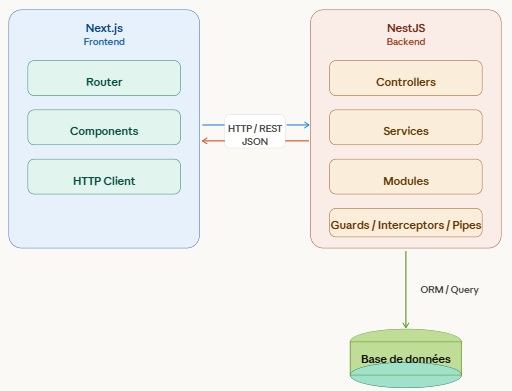
\includegraphics[width=0.7\textwidth,keepaspectratio]{Images/architecture.png}
\caption{Architecture physique de SolidMaint}
\label{fig:architecture_physique}
\end{figure}

\subsection{Architecture logique}
Nous avons choisi comme architecture logicielle l'\textbf{architecture monolithique
modulaire}. Ce choix est basé sur la combinaison entre la simplicité et la robustesse
des applications monolithiques traditionnelles, tout en bénéficiant de la clarté
structurelle des architectures orientées modules.

L'architecture du \textbf{monolithe modulaire} nous permet de travailler dans une
base de code unifiée, avec des frontières clairement définies et des modules
indépendants. Elle consiste à diviser le système en plusieurs modules fonctionnels
cohésifs, chacun encapsulant sa propre logique métier, ses contrôleurs, ses services
et ses DTOs.

Nous avons choisi cette architecture afin de maintenir l'indépendance des modules et
d'obtenir une grande cohésion, une encapsulation des données, ainsi qu'une
focalisation sur les fonctionnalités métiers, tout en conservant la simplicité de
déploiement d'un monolithe.

\begin{figure}[H]
\centering
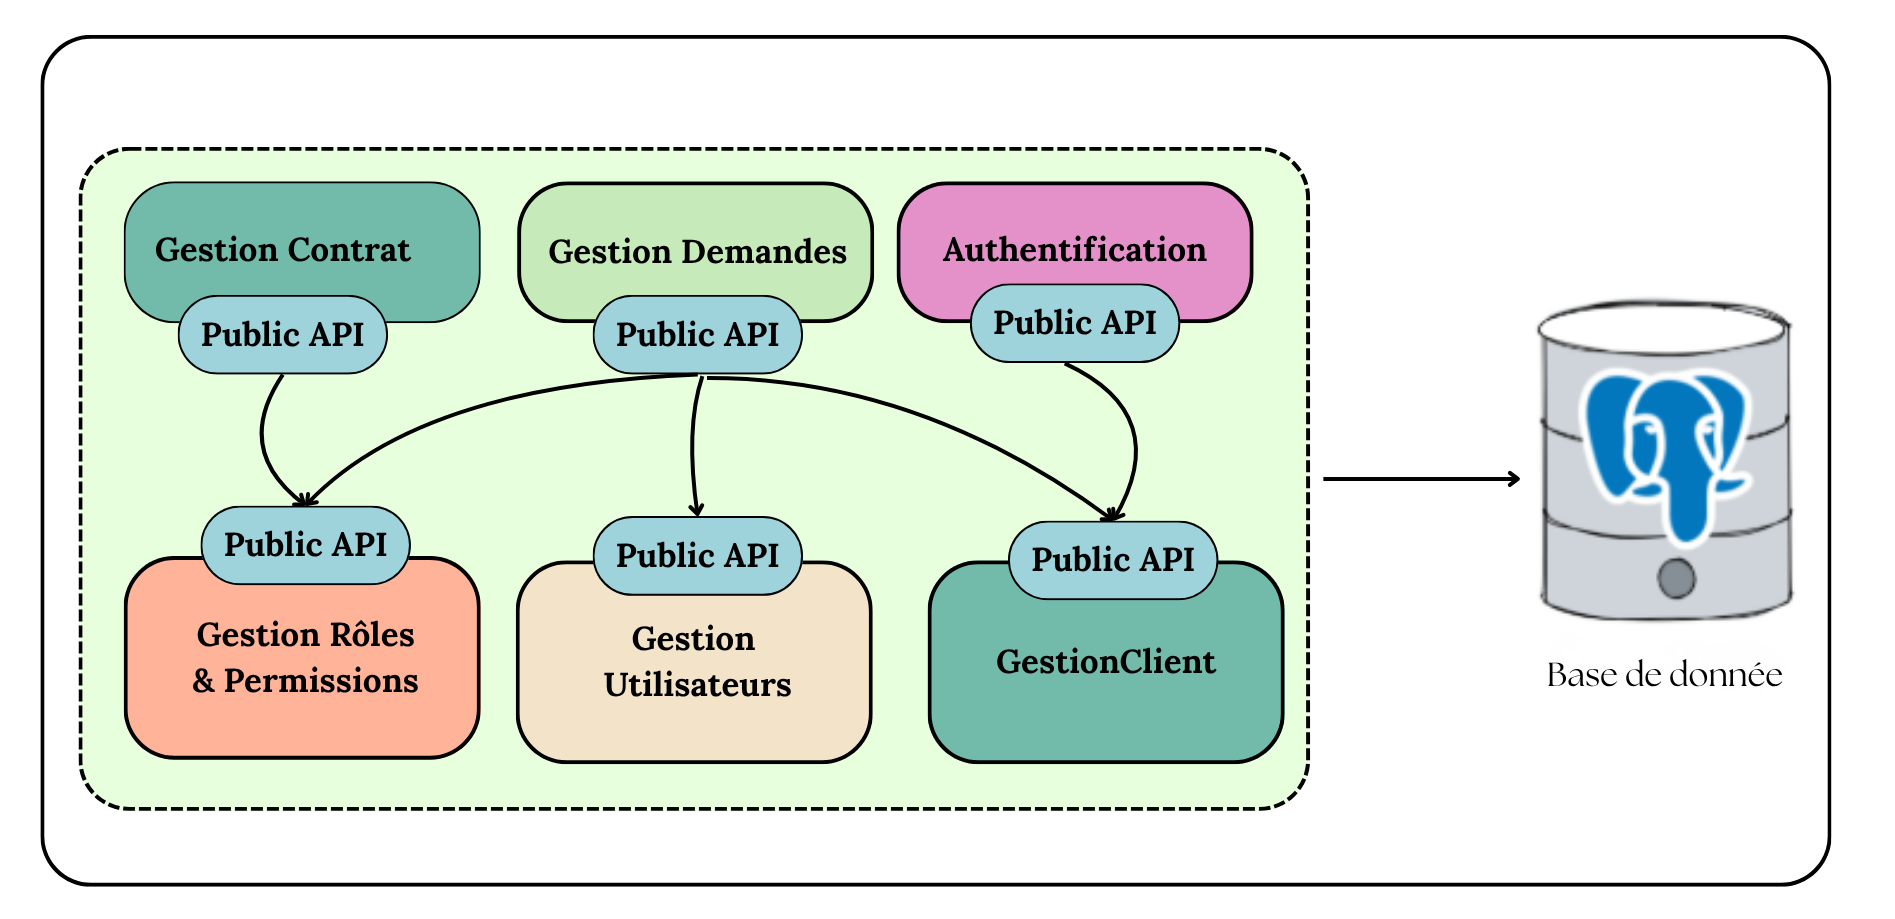
\includegraphics[width=0.7\textwidth,keepaspectratio]{Images/Modular Monoith.png}
\caption{Architecture monolithique modulaire}
\label{fig:architecture_modulaire}
\end{figure}

%─────────────────────────────────────────────────────────────────────────────
% CONCLUSION
%─────────────────────────────────────────────────────────────────────────────

\section{Conclusion}
Ce chapitre a établi les fondements techniques et méthodologiques de notre projet
\textbf{SolidMaint}. L'identification des six acteurs et la spécification des besoins
fonctionnels et non fonctionnels ont permis de définir précisément les exigences de
la plateforme. La modélisation UML et l'approche de pilotage Scrum avec la
planification en quatre sprints structurent la démarche de développement.

L'environnement de développement choisi et l'architecture modulaire garantissent une solution robuste et évolutive. Ces éléments constituent la base solide pour aborder la phase de réalisation.
\newline Le chapitre suivant détaillera l'implémentation du premier sprint consacré à la gestion des utilisateurs et authentification.



% ---- Chapitre 3 ----
\hiddenpart{Sprint 1 -- Socle Sécurité et Contrôle d'Accès}
\chaptercover{3}{Sprint 1 -- Socle Sécurité et Contrôle d'Accès}
\section*{Introduction}
Dans le chapitre précédent, nous avons défini les besoins liés à notre solution et réparti les différentes tâches du projet afin que les phases de travail soient correctement planifiées.
\newline Au cours de ce chapitre, nous présenterons les fonctionnalités liées  à la gestion des utilisateurs, à l'authentification et au contrôle d'accès basé sur les rôles (RBAC), retenues dans le cadre du premier sprint de notre projet.

% ─────────────────────────────────────────────────────────────────────────────
% SECTION 1 : BACKLOG DU SPRINT 1
% ─────────────────────────────────────────────────────────────────────────────
\section{Sprint Planning Meeting }
La planification du sprint est essentielle à la réussite de notre solution, au bout de laquelle on clarifie les différentes fonctionnalités à implémenter lors du sprint à venir. Cette partie est efficace afin de préparer des objectifs clairs.
L'objectif de ce sprint est de mettre en place les fondations fonctionnelles et
sécuritaires de la solution, en implémentant les mécanismes d'authentification et
de sécurisation des accès ainsi que les fonctionnalités de gestion des utilisateurs
et de leurs profils. Il s'agit également d'assurer un contrôle efficace des accès
et des permissions en introduisant l'administration du système à travers la gestion
des comptes utilisateurs, des rôles et des permissions (RBAC).
\subsection{Backlog du premier sprint}
\label{sec:backlog_sprint1}

Voici l'ensemble des fonctionnalités issues du Product Backlog, qui seront réalisées dans le cadre de ce sprint.
\newline
\textbf{1 : Effort faible, 2 : Effort moyen, 3 : Effort élevé}
\rowcolors{0}{}{}
\arrayrulecolor{black}
\renewcommand{\arraystretch}{1.3}
\small

\begin{longtable}{|C{1cm}|m{6.5cm}|m{7cm}|C{1cm}|}
\hline
\textbf{ID US} & \textbf{User Story} & \textbf{Description technique} & \textbf{Effort} \\
\hline
\endfirsthead

    \hline

\endhead

\hline
\endfoot

\hline
\endlastfoot

% Epic 1: Authentification et Sécurité
\multicolumn{4}{|l|}{\cellcolor{blue!20}\textbf{Epic 1 - Authentification et Sécurité}} \\
\hline

US01 & En tant qu'\textbf{utilisateur}, je souhaite m'authentifier avec email et mot de passe afin d'accéder à mes informations de manière sécurisée. & 
\vspace{2mm}
\begin{itemize}[nosep, left=0pt, label={$\bullet$}]
\item Développer l'endpoint \texttt{POST /api/auth/login}
\item Mettre en place la gestion de session via \textbf{JWT}
    (access token 15 min, refresh token 7 jours stocké en base)
\item Réaliser l'interface connexion login
\item Consommer l'API d'authentification
\item Gérer les tentatives échouées (3 essais) avec verrouillage temporaire
\end{itemize} & 2 \\
\hline

US02 & En tant qu'\textbf{utilisateur}, je souhaite réinitialiser mon mot de passe afin de retrouver l'accès à mon compte. & 
\vspace{2mm}
\begin{itemize}[nosep, left=0pt, label={$\bullet$}]
\item Développer les endpoints
    \texttt{POST /api/auth/mot-de-passe-oublie} et
    \texttt{POST /api/auth/reinitialiser-mot-de-passe}
  \item Créer les formulaires « mot de passe oublié » et
    de réinitialisation côté Next.js
  \item Générer un token sécurisé (bcrypt) avec expiration
    de \textbf{1 heure}, stocké dans
    \texttt{TokenReinitialisationMotDePasse}
  \item Invalider les anciens tokens non utilisés à chaque
    nouvelle demande
  \item Configurer l'envoi d'un e-mail de réinitialisation
    et d'un e-mail de confirmation via \textbf{Nodemailer}
\end{itemize} & 2 \\
\hline

US03 & En tant qu'\textbf{utilisateur}, je souhaite m'authentifier via Google ou GitHub afin de me connecter rapidement sans créer de compte. & 
\vspace{2mm}
\begin{itemize}[nosep, left=0pt, label={$\bullet$}]
\item Intégrer les stratégies OAuth2 via
    \texttt{passport-google-oauth20} et \texttt{passport-github2}
    dans NestJS (\texttt{@nestjs/passport})
\item Implémenter les routes \texttt{GET /api/auth/google},\texttt{GET /api/auth/github} et leurs callbacks
  \item Si l'utilisateur existe en base et est actif :
    générer les tokens JWT et rediriger vers le frontend
    avec \texttt{?oauth=success}
\item Vérifier l'existence de l'utilisateur en base de données et une demande d'inscription OAuth est envoyée à l'admin
\item Implémenter les routes /auth/google, /auth/github et leurs callbacks, avec génération d'un JWT
\item Implémenter les boutons OAuth sur la page de login
\end{itemize} & 3 \\
\hline

US04 & En tant qu'\textbf{utilisateur}, je souhaite me déconnecter de la plateforme afin de sécuriser ma session. & 
\vspace{2mm}
\begin{itemize}[nosep, left=0pt, label={$\bullet$}]
\item Développer l'endpoint POST /auth/logout avec révocation du refresh token en base
\item Supprimer \texttt{accessToken}, \texttt{refreshToken}
    et \texttt{user} du \texttt{localStorage}
\item Vider le cache React Query (\texttt{queryClient.clear()})
\item Réaliser le bouton de déconnexion 
\end{itemize} & 1 \\
\hline

US05 & En tant qu'\textbf{utilisateur}, je souhaite que mon compte soit protégé contre les tentatives de connexion malveillantes afin de garantir la sécurité de mes données. & 
\vspace{2mm}
\begin{itemize}[nosep, left=0pt, label={$\bullet$}]
  \item Implémenter le compteur de tentatives échouées
    (\texttt{tentativesConnexionEchouees}) en base de données
  \item Verrouiller le compte après \textbf{3 tentatives échouées}
    pendant \textbf{1 minute} via le champ
    \texttt{compteVerrouilleJusquA}
  \item Réinitialiser le compteur à 0 après une connexion réussie
  \item Appliquer le rate limiting global via
    \texttt{@nestjs/throttler} sur les endpoints publics
\end{itemize} & 2 \\
\hline

% Epic 2: Gestion des utilisateurs
\multicolumn{4}{|l|}{\cellcolor{blue!20}\textbf{Epic 2 - Gestion des utilisateurs}} \\
\hline

US06 & En tant qu'\textbf{utilisateur}, je souhaite gérer mon profil afin que mes informations soient toujours à jour. & 
\vspace{2mm}
\begin{itemize}[nosep, left=0pt, label={$\bullet$}]
\item Développer les endpoints \texttt{GET /api/profil} et \texttt{PUT /api/profil}
\item Implémenter l'upload de la photo de profil \texttt{POST /api/profil/upload-photo}
\item Développer le changement de mot de passe via
    \texttt{POST /api/profil/change-password}
    avec vérification de l'ancien mot de passe (bcrypt)
\item Gérer les e-mails secondaires :
    \texttt{GET/POST/DELETE /api/profil/emails} et
    \texttt{PATCH /api/profil/emails/principal}
\item Réaliser l'interface profil côté Next.js  avec formulaire prérempli
\end{itemize} & 2 \\
\hline

US07 & En tant qu'\textbf{administrateur}, je souhaite créer des utilisateurs afin de gérer les accès au système. & 
\vspace{2mm}
\begin{itemize}[nosep, left=0pt, label={$\bullet$}]
\item Développer l'endpoint \texttt{POST /api/users}
\item Générer automatiquement un mot de passe temporaire haché via \textbf{bcrypt} (facteur 10)
\item Générer un token de réinitialisation (1 heure) et construire le lien de réinitialisation
\item Créer automatiquement le \texttt{ProfilEmploye}
    avec matricule \texttt{EMP-\{id\}} si le rôle n'est pas CLIENT
\item Valider les données d'entrée via \textbf{class-validator}
  \item Envoyer un e-mail de bienvenue via \textbf{Nodemailer}
    contenant le mot de passe temporaire et le lien de
    réinitialisation
  \item Réaliser le formulaire d'ajout côté Next.js
\end{itemize} & 3 \\
\hline

US08 & En tant qu'\textbf{administrateur}, je souhaite modifier les informations d'un utilisateur afin de maintenir des données à jour. & 
\vspace{2mm}
\begin{itemize}[nosep, left=0pt, label={$\bullet$}]
\item Développer l'endpoint \texttt{PUT /api/users/:id}
\item Sécuriser l'accès à l'endpoint pour les administrateurs uniquement
\item Valider les données via \textbf{class-validator}
\item Réaliser le formulaire de modification côté Next.js
\end{itemize} & 2 \\
\hline

US09 & En tant qu'\textbf{administrateur}, je souhaite activer et désactiver un compte utilisateur afin de contrôler l'accès au système. & 
\vspace{2mm}
\begin{itemize}[nosep, left=0pt, label={$\bullet$}]
\item Développer les endpoints \texttt{PATCH /api/users/:id/desactiver} et \texttt{PATCH /api/users/:id/reactiver}
\item Implémenter les vérifications de réassignation des tickets et des demandes en cas de désactivation
\item Envoyer des notifications pour informer l'utilisateur de l'activation ou désactivation de son compte
\item Réaliser les boutons d'action avec appels des API
\end{itemize} & 3 \\
\hline

US10 & En tant qu'\textbf{administrateur}, je souhaite consulter la liste des utilisateurs afin de visualiser et gérer efficacement les comptes. & 
\vspace{2mm}
\begin{itemize}[nosep, left=0pt, label={$\bullet$}]
\item Développer l'endpoint \texttt{GET /api/users}
\item Réaliser l'interface d'administration avec vue grille
    et vue liste, filtres par statut et par rôle,
    barre de recherche dynamique

\end{itemize} & 1 \\
\hline

US11 & En tant qu'\textbf{utilisateur}, je souhaite consulter l'historique de mes activités afin de suivre mes actions dans le système. & 
\vspace{2mm}
\begin{itemize}[nosep, left=0pt, label={$\bullet$}]
\item Développer l'endpoint \texttt{GET /api/users/:id/activities} pour récupérer l'historique
\item Implémenter la logique de filtrage dans le backend en utilisant l'opérateur contains
\item Implémenter une barre de recherche dynamique
\item Réaliser l'interface timeline avec filtres par date et type d'action
\end{itemize} & 2 \\
\hline

% Epic 3: Gestion des rôles et permissions
\multicolumn{4}{|l|}{\cellcolor{blue!20}\textbf{Epic 3 - Gestion des rôles et permissions}} \\
\hline

US12 & En tant qu'\textbf{administrateur}, je souhaite gérer des rôles afin de structurer les accès au système. & 
\vspace{2mm}
\begin{itemize}[nosep, left=0pt, label={$\bullet$}]
\item Développer les endpoints CRUD pour la gestion complète des rôles
\item Implémenter le PermissionsGuard et le décorateur @Permissions pour sécuriser les routes du backend 
\item Réaliser l'interface de gestion sous forme de matrice
\end{itemize} & 3 \\
\hline

US13 & En tant qu'\textbf{administrateur}, je souhaite attribuer des permissions granulaires aux rôles afin de contrôler précisément les accès. & 
\vspace{2mm}
\begin{itemize}[nosep, left=0pt, label={$\bullet$}]
\item Développer l’endpoint PATCH /roles-permissions/roles/:id/sync pour synchroniser dynamiquement les associations entre un rôle et ses permissions. 
\item Implémenter la logique de mise à jour atomique                                                                                                                                                                                                                       
\item Développer l'interface interactive de type "Matrice de contrôle d'accès" 

\end{itemize} & 2 \\
\hline
US14 & En tant qu'\textbf{administrateur}, je souhaite consulter la matrice rôles-permissions afin de visualiser rapidement les droits de chaque rôle. & 
\vspace{2mm}
\begin{itemize}[nosep, left=0pt, label={$\bullet$}]
\item Développer l’endpoint GET /roles-permissions/matrix ) pour récupérer les données 
\item Implémenter la logique de structuration des données au format JSON                
\item Réaliser l’interface de visualisation de type "Heatmap" ou "Tableau de bord"

\end{itemize} & 3 \\
\hline

% Epic 4: Demandes d'inscription OAuth
\multicolumn{4}{|l|}{\cellcolor{blue!20}\textbf{Epic 4 - Demandes d'inscription OAuth}} \\
\hline

US15 & En tant qu'\textbf{utilisateur externe}, je souhaite demander l'accès via OAuth afin de m'inscrire facilement. & 
\vspace{2mm}
\begin{itemize}[nosep, left=0pt, label={$\bullet$}]
\item Développer l'endpoint POST /auth/oauth/request pour créer une demande
\item Enregistrer la demande en base avec statut EN\_ATTENTE
\item Implémenter l'envoi de notification à l'administrateur via email et in-app
\item Réaliser l'interface de demande d'accès
\end{itemize} & 3 \\
\hline

US16 & En tant qu'\textbf{administrateur}, je souhaite valider ou rejeter les demandes d'inscription OAuth afin de contrôler les accès. & 
\vspace{2mm}
\begin{itemize}[nosep, left=0pt, label={$\bullet$}]
\item Développer les endpoints PATCH /auth/oauth/requests/:id/approve et /reject
\item Implémenter la création automatique du compte utilisateur lors de l'approbation
\item Configurer l'envoi d'emails de confirmation ou rejet via Nodemailer
\item Réaliser l'interface de gestion des demandes avec actions d'approbation/rejet
\end{itemize} & 3 \\
\hline
% Epic 4: Demandes d'inscription OAuth


\end{longtable}



% ─────────────────────────────────────────────────────────────────────────────
% SECTION 2 : ANALYSE
% ─────────────────────────────────────────────────────────────────────────────

\section{Analyse}
Dans le processus de développement, l'analyse joue un rôle important ; elle permet d'identifier les exigences du système et de traduire les besoins exprimés en spécifications claires et cohérentes.
C'est pour cela que nous allons présenter les diagrammes ainsi que les tableaux descriptifs des cas d'utilisation
\label{sec:analyse_sprint1}

\subsection{Diagramme des cas d'utilisation du premier sprint}

La figure ci-dessous présente le diagramme de cas d'utilisation du premier sprint : 
\begin{figure}[htbp]
        \centering
        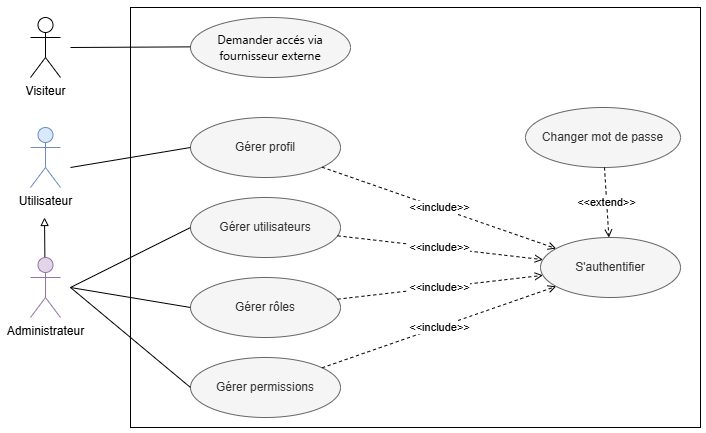
\includegraphics[width=0.75\textwidth,height=0.65\textheight,keepaspectratio]{Images/Diagramme_cas_utilisation_sprint1.png}
        \caption{Diagramme des cas d'utilisation du premier sprint}
        \label{fig:use_case_sprint1}
\end{figure}

Nous allons accompagner les cas d'utilisation d'un texte descriptif pour expliquer le scénario de chaque cas ainsi que ses exceptions.

\subsection{Description textuelle de cas d'utilisation «S'authentifier»}
La figure ci-dessous présente la description textuelle de cas d'utilisation «S'authentifier» :

\footnotesize
\renewcommand{\arraystretch}{0.95}
\begin{longtable}{|P{3.5cm}|P{10.5cm}|}
\caption{Description textuelle du cas d'utilisation « S'authentifier »} \\
\hline
\endfirsthead
\hline
\endhead
\hline
\endfoot
\hline
\endlastfoot
\textbf{Nom du cas d'utilisation} & S'authentifier \\
\hline
\textbf{Acteurs} & Utilisateur \\
\hline
\textbf{Préconditions} & L'utilisateur dispose déjà d'un compte actif \\
\hline
\textbf{Postconditions} & L'utilisateur est authentifié et reçoit un jeton d'accès ainsi qu'un jeton de rafraîchissement \\
\hline
\textbf{Scénario principal} &
\begin{minipage}[t]{\linewidth}\raggedright
\begin{enumerate}[label=\arabic*., nosep,leftmargin=0.6cm,topsep=0pt,itemsep=1pt]
\item Le système affiche le formulaire de connexion.
\item L'utilisateur saisit son adresse e-mail et son mot de passe.
\item L'utilisateur valide la connexion.
\item Le système vérifie l'existence du compte.
\item Le système vérifie la validité du mot de passe.
\item Le système vérifie que le compte est actif.
\item Le système détermine le profil de l'utilisateur et récupère ses rôles et permissions.
\item Le système met à jour la date de dernière connexion.
\item Le système génère un jeton d'accès et un jeton de rafraîchissement.
\item Le système renvoie les informations de l'utilisateur connecté.
\item Le système redirige l'utilisateur vers la page d'accueil ou le tableau de bord.
\end{enumerate}
\end{minipage} \\
\hline
\textbf{Scénarios alternatifs} &
\begin{itemize}[nosep,leftmargin=0.6cm,topsep=0pt,itemsep=1pt, label=$\bullet$]
\item L'utilisateur s'authentifie via Google.
\item L'utilisateur s'authentifie via GitHub.
\end{itemize} \\
\hline
\textbf{Scénarios d'exception} &
\begin{itemize}[nosep,leftmargin=0.6cm,topsep=0pt,itemsep=1pt, label=$\bullet$]
\item L'utilisateur saisit un identifiant inexistant.
\item L'utilisateur saisit un mot de passe incorrect.
\item Le compte de l'utilisateur est désactivé.
\item Le formulaire contient des champs obligatoires vides ou invalides.
\item Le compte est temporairement verrouillé après \textbf{3 tentatives échouées} consécutives (durée : 1 minute).
\end{itemize} \\
\hline
\end{longtable}
\normalsize
\vspace{-0.3cm}


\subsection{Description textuelle de cas d'utilisation « Changer mot de passe »}
La figure ci-dessous présente la description textuelle du cas d'utilisation « Changer le mot de passe » :

\footnotesize
\renewcommand{\arraystretch}{0.95}
\begin{longtable}{|P{3.5cm}|P{10.5cm}|}
\caption{Description textuelle de cas d'utilisation « Changer mot de passe »} \\
\hline
\endfirsthead
\hline
\endhead
\hline
\endfoot
\hline
\endlastfoot
\textbf{Nom du cas d'utilisation} & Changer mot de passe \\
\hline
\textbf{Acteurs} & Utilisateurs \\
\hline
\textbf{Préconditions} & L'utilisateur possède déjà un compte \\
\hline
\textbf{Postconditions} & Le mot de passe est réinitialisé \\
\hline
\textbf{Scénario principal} &
\begin{minipage}[t]{\linewidth}\raggedright
\begin{enumerate}[label=\arabic*., nosep,leftmargin=0.6cm,topsep=0pt,itemsep=1pt]
\item Le système affiche un formulaire de changement de mot de passe.
\item L'utilisateur saisit son e-mail.
\item L'utilisateur clique sur le bouton « Réinitialiser le mot de passe ».
\item Le système vérifie l'existence de l'email.
\item Le système envoie un e-mail à l'utilisateur.
\item L'utilisateur clique sur le lien reçu par e-mail.
\item Le système affiche le formulaire de réinitialisation de mot de passe.
\item L'utilisateur saisit son nouveau mot de passe deux fois pour confirmation.
\item Le système valide et enregistre le nouveau mot de passe.
\item Le système envoie un e-mail de confirmation à l'utilisateur.
\end{enumerate}
\end{minipage} \\
\hline
\textbf{Scénarios d'exception} &
\begin{itemize}[nosep,leftmargin=0.6cm,topsep=0pt,itemsep=1pt, label=$\bullet$]
\item L'utilisateur saisit un e-mail qui ne correspond à aucun compte existant.
\item L'utilisateur a rempli un champ invalide, ou a laissé un champ vide.
\item Le lien de réinitialisation est expiré.
\item L'utilisateur ne confirme pas correctement le mot de passe.
\end{itemize} \\
\hline
\end{longtable}
\normalsize
\vspace{-0.3cm}

\subsection{Analyse de la fonctionnalité « Demander accès via fournisseur externe »}
Dans cette partie, nous allons présenter les cas d'utilisation raffinés relatifs à la demande d'accès via fournisseur externe afin de comprendre les différentes étapes du processus d'inscription et d'authentification.

\subsubsection{Raffinement de cas d'utilisation « Demander accés via fournisseur externe »}
Au cours de cette partie, nous allons analyser les sous-cas d'utilisation pour le processus d'authentification OAuth :

\begin{figure}[htbp]
        \centering
        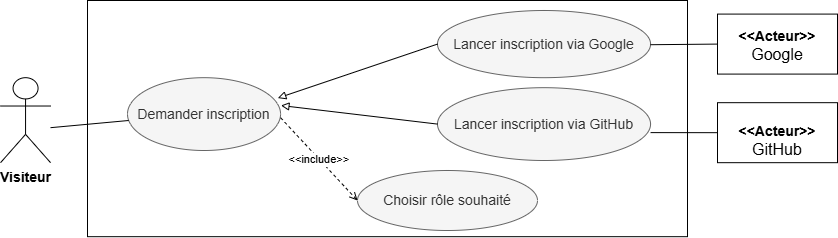
\includegraphics[width=0.75\textwidth,height=0.65\textheight,keepaspectratio]{Images/demande insc.png}
        \caption{Raffinement de cas d'utilisation « Demander accés via fournisseur externe »}
        \label{fig:oauth_refinement}
\end{figure}

\subsubsection{Description textuelle de cas d'utilisation « Soumettre demande d'inscription »}

\footnotesize
\renewcommand{\arraystretch}{0.95}
{\sloppy
\begin{longtable}{|P{3.5cm}|P{10.5cm}|}
\caption{Description textuelle « Soumettre demande d'inscription »} \\
\hline
\endfirsthead
\hline
\endhead
\hline
\endfoot
\hline
\endlastfoot
\textbf{Nom du cas d'utilisation} & Soumettre demande d'inscription \\
\hline
\textbf{Acteurs} & Visiteur \\
\hline
\textbf{Préconditions} & Le visiteur n'a pas de compte actif dans le système et a accès à la page d'authentification \\
\hline
\textbf{Postconditions} &
\begin{minipage}[t]{\linewidth}\raggedright\hyphenpenalty=1000
La demande d'inscription est créée, enregistrée avec le statut \textbf{EN\_ATTENTE}, et les administrateurs sont notifiés
\end{minipage} \\\hline
\textbf{Scénario principal} &
\begin{minipage}[t]{\linewidth}\raggedright
\begin{enumerate}[label=\arabic*., leftmargin=0.6cm, nosep, itemsep=1pt]
\item Le visiteur accède à la page de connexion / inscription.
\item Le visiteur sélectionne le rôle souhaité : Client, Développeur ou Chef de projet.
\item Le visiteur clique sur « Se connecter avec Google » ou « Se connecter avec GitHub ».
\item Le système redirige le visiteur vers le fournisseur OAuth sélectionné.
\item Le visiteur s'authentifie et autorise l'application à accéder à ses informations de base.
\item Le fournisseur OAuth redirige le visiteur vers l'application avec un code d'autorisation.
\item Le système récupère les informations du profil OAuth et vérifie s'il existe déjà un compte actif associé.
\item Si aucun compte actif n'existe, le système crée une demande d'inscription avec le statut \textit{EN ATTENTE}.
\item Le système envoie une \textbf{notification interne} et un \textbf{e-mail} à chaque administrateur actif pour l'informer de la nouvelle demande d'inscription.
\item Le système envoie un \textbf{e-mail de confirmation au visiteur} indiquant que sa demande a bien été reçue et est en cours d'examen.
\item Le système affiche un message d'attente à l'écran.
\end{enumerate}
\end{minipage} \\
\hline
\textbf{Scénarios alternatifs} &
\begin{itemize}[nosep,leftmargin=0.6cm,topsep=0pt,itemsep=1pt, label=$\bullet$]
\item Compte actif déjà existant : le système connecte directement l'utilisateur sans créer de nouvelle demande.
\item Demande déjà soumise pour le même e-mail et le même fournisseur : le système conserve la demande existante et affiche un message d'information, sans créer de doublon.
\item Annulation de l'autorisation OAuth : le visiteur est redirigé vers la page d'authentification sans création de demande.
\end{itemize} \\
\hline
\textbf{Scénarios d'exception} &
\begin{itemize}[nosep,leftmargin=0.6cm,topsep=0pt,itemsep=1pt, label=$\bullet$]
\item Le fournisseur OAuth ne fournit pas l'adresse e-mail : le système affiche un message d'erreur et interrompt le traitement.
\item Le fournisseur OAuth est indisponible : le système affiche un message d'erreur technique.
\item Le visiteur refuse l'accès aux données OAuth : le système annule le flux et revient à l'écran d'authentification.
\end{itemize} \\
\hline
\end{longtable}
}
\normalsize
\vspace{-0.3cm}

\subsubsection{Description textuelle de cas d'utilisation « Valider demande »}

\footnotesize
\renewcommand{\arraystretch}{0.95}
\begin{longtable}{|P{3.5cm}|P{10.5cm}|}
\caption{Description textuelle « Valider demande »} \\
\hline
\endfirsthead
\hline
\endhead
\hline
\endfoot
\hline
\endlastfoot
\textbf{Nom du cas d'utilisation} & Valider demande \\
\hline
\textbf{Acteurs} & Administrateur \\
\hline
\textbf{Préconditions} & L'administrateur est authentifié et possède la permission de traiter les demandes d'inscription \\
\hline
\textbf{Postconditions} & Le compte utilisateur est créé et activé, la demande est marquée \textit{APPROUVEE}, et l'utilisateur est notifié \\
\hline
\textbf{Scénario principal} &
\begin{minipage}[t]{\linewidth}\raggedright
\begin{enumerate}[label=\arabic*., leftmargin=0.6cm, nosep, itemsep=1pt]
\item L'administrateur accède au module de gestion des demandes d'inscription.
\item Le système affiche la liste des demandes en attente.
\item L'administrateur sélectionne une demande à traiter.
\item Le système affiche les informations du demandeur récupérées via OAuth.
\item L'administrateur clique sur « Approuver ».
\item Le système crée le compte utilisateur à partir des informations de la demande.
\item Le système attribue le rôle correspondant à l'utilisateur.
\item Le système marque la demande comme \textit{APPROUVEE}.
\item Le système envoie un e-mail de confirmation à l'utilisateur.
\item Le système affiche un message de succès à l'administrateur.
\end{enumerate}
\end{minipage} \\
\hline
\textbf{Scénarios alternatifs} &
\begin{itemize}[nosep,leftmargin=0.6cm,topsep=0pt,itemsep=1pt, label=$\bullet$]
\item L'administrateur clique sur « Refuser » : le système ouvre une boîte de dialogue pour saisir un motif de refus puis traite la demande comme rejetée.
\item Un compte avec le même e-mail existe déjà : le système signale le conflit et empêche la création d'un doublon.
\item La demande a déjà été traitée : le système affiche un message d'information et empêche une nouvelle validation.
\end{itemize} \\
\hline
\textbf{Scénarios d'exception} &
\begin{itemize}[nosep,leftmargin=0.6cm,topsep=0pt,itemsep=1pt, label=$\bullet$]
\item Erreur lors de la création du compte : le système annule l'opération et affiche un message d'erreur.
\item Erreur lors de l'envoi de l'e-mail : le compte peut être créé, mais le système journalise l'incident et affiche un avertissement.
\item Données de finalisation incomplètes : le système refuse la validation et demande de compléter les champs obligatoires.
\end{itemize} \\
\hline
\end{longtable}
\normalsize
\vspace{-0.3cm}

\subsection{Analyse de la fonctionnalité « Gérer utilisateurs »}
Dans cette partie, nous allons présenter les cas d'utilisation relatifs à la gestion des utilisateurs afin de comprendre les principales fonctionnalités du système, ce qui permet d'avoir une vue globale des interactions.
\subsubsection{Raffinement de cas d'utilisation « Gérer utilisateurs »}
Au cours de cette partie, nous allons analyser chaque cas d'utilisation raffiné pour le cas de gestion des utilisateurs :    

\begin{figure}[htbp]
        \centering
        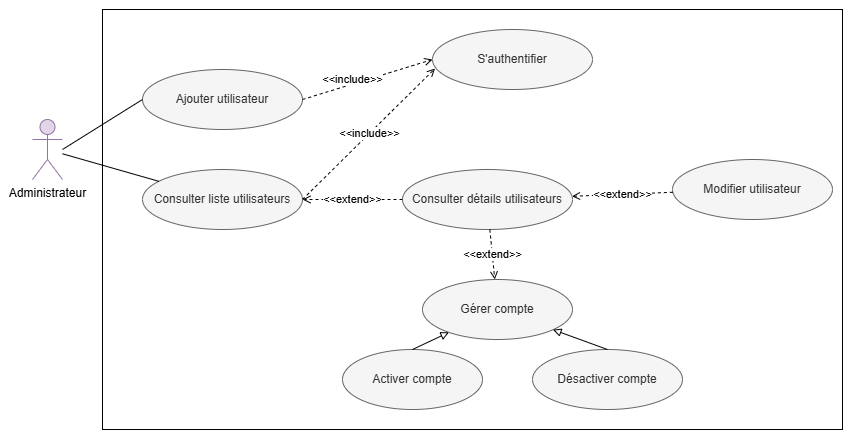
\includegraphics[width=0.8\textwidth,keepaspectratio]{Images/Gérer utilisateur.drawio.png}
        \caption{Diagramme des cas d'utilisation « Gérer utilisateurs »}
        \label{fig:gerer_utilisateurs}
\end{figure}

% \subsubsection{Description textuelle de cas d'utilisation « Consulter liste utilisateurs »}
% 
% \footnotesize
% \renewcommand{\arraystretch}{0.95}
% \begin{longtable}{|P{3.5cm}|P{10.5cm}|}
% \caption{Description textuelle « Consulter liste utilisateurs »} \\
% \hline
% \endfirsthead
% \hline
% \endhead
% \hline
% \endfoot
% \hline
% \endlastfoot
% \textbf{Nom du cas d'utilisation} & Consulter liste utilisateurs \\
% \hline
% \textbf{Acteurs} & Administrateur \\
% \hline
% \textbf{Préconditions} & L'utilisateur est authentifié\newline L'utilisateur possède la permission de consulter les utilisateurs \\
% \hline
% \textbf{Postconditions} & Liste des utilisateurs affichée \\
% \hline
% \textbf{Scénario principal} &
% \begin{minipage}[t]{\linewidth}
% \begin{enumerate}[label=\arabic*., leftmargin=0.6cm, nosep, itemsep=1pt]
%     \item L'administrateur accède à la section "Utilisateurs".
%     \item Le système affiche les utilisateurs sous forme de grille (par défaut) ou de liste selon le choix de l'utilisateur.
%     \item L'administrateur recherche un utilisateur en saisissant des informations clés dans la barre de recherche ou par des boutons de filtre (par statut, par rôle).
%     \item Le système filtre la liste.
% \end{enumerate}
% % \end{minipage} \\
% \hline
% \textbf{Scénarios alternatifs} & L'administrateur clique sur le bouton « Exporter ». \\
% \hline
% \end{longtable}
% \normalsize
% \vspace{-0.3cm}

\subsubsection{Description textuelle de cas d'utilisation « Ajouter utilisateur »}

\footnotesize
\renewcommand{\arraystretch}{0.95}
\begin{longtable}{|P{3.5cm}|P{10.5cm}|}
\caption{Description textuelle « Ajouter utilisateur »} \\
\hline
\endfirsthead
\hline
\endhead
\hline
\endfoot
\hline
\endlastfoot
\textbf{Nom du cas d'utilisation} & Ajouter utilisateur \\
\hline
\textbf{Acteurs} & Administrateur \\
\hline
\textbf{Préconditions} & L'utilisateur est authentifié\newline L'utilisateur possède la permission de créer des utilisateurs\newline Liste des utilisateurs affichée \\
\hline
\textbf{Postconditions} & Utilisateur est ajouté \\
\hline
\textbf{Scénario principal} &
\begin{minipage}[t]{\linewidth}\raggedright
\begin{enumerate}[label=\arabic*., leftmargin=0.6cm, nosep, itemsep=1pt]
    \item L'administrateur clique sur le bouton "Nouvel Utilisateur".
    \item Le système affiche le formulaire d'ajout.
    \item L'administrateur remplit le formulaire.
    \item L'administrateur valide le formulaire en cliquant sur (Créer le compte).
    \item Le système affiche le message de succès.
\end{enumerate}
\end{minipage} \\
\hline
\textbf{Scénarios d'exception} &
\begin{itemize}[nosep,leftmargin=0.6cm,topsep=0pt,itemsep=1pt, label=$\bullet$]
\item L'administrateur a rempli un champ invalide, ou a laissé un champ vide.
\item L'administrateur saisit un e-mail déjà utilisé dans un autre compte.
\item L'administrateur tente de fermer la fenêtre alors qu'il a commencé à saisir des données.
\end{itemize} \\
\hline
\textbf{Scénarios alternatifs} & Le système génère un mot de passe temporaire. \\
\hline
\end{longtable}
\normalsize
\vspace{-0.3cm}

\subsubsection{Description textuelle de cas d'utilisation « Désactiver un utilisateur »}

\footnotesize
\renewcommand{\arraystretch}{0.95}
\begin{longtable}{|P{3.5cm}|P{10.5cm}|}
\caption{Description textuelle « Désactiver un utilisateur »} \\
\hline
\endfirsthead
\hline
\endhead
\hline
\endfoot
\hline
\endlastfoot
\textbf{Nom du cas d'utilisation} & Désactiver un utilisateur \\
\hline
\textbf{Acteurs} & Administrateur \\
\hline
\textbf{Préconditions} & L'utilisateur est authentifié\newline L'utilisateur possède la permission de désactiver les utilisateurs\newline Liste des utilisateurs affichée\newline L'utilisateur à désactiver doit être actuellement Actif \\
\hline
\textbf{Postconditions} & Le compte est désactivé \\
\hline
\textbf{Scénario principal} &
\begin{minipage}[t]{\linewidth}\raggedright
\begin{enumerate}[label=\arabic*., leftmargin=0.6cm, nosep, itemsep=1pt]
    \item L'administrateur choisit un compte dans la liste.
    \item L'administrateur clique sur l'action (Désactiver).
    \item Le système vérifie si l'utilisateur possède des tickets actifs ou des demandes en attente.
    \item Le système affiche une boîte de dialogue de confirmation.
    \item L'administrateur confirme l'action.
    \item Le système met à jour le statut de l'utilisateur.
    \item Le système envoie un e-mail automatique à l'utilisateur pour l'informer de la suspension de son compte.
\end{enumerate}
\end{minipage} \\
\hline
\textbf{Scénarios alternatifs} & L'administrateur réassigne les tickets ou les demandes. \\
\hline
\textbf{Scénarios d'exception} &
\begin{itemize}[nosep,leftmargin=0.6cm,topsep=0pt,itemsep=1pt, label=$\bullet$]
\item L'utilisateur tente de désactiver un utilisateur qui possède des tickets actifs ou des demandes en attente.
\end{itemize} \\
\hline
\end{longtable}
\normalsize
\vspace{-0.3cm}

\subsubsection{Description textuelle de cas d'utilisation « Modifier Profil »}

\footnotesize
\renewcommand{\arraystretch}{0.95}
\begin{longtable}{|P{3.5cm}|P{10.5cm}|}
\caption{Description textuelle « Modifier le Profil »} \\
\hline
\endfirsthead
\hline
\endhead
\hline
\endfoot
\hline
\endlastfoot
\textbf{Nom du cas d'utilisation} & Modifier le Profil \\
\hline
\textbf{Acteurs} & Administrateur, Utilisateur \\
\hline
\textbf{Préconditions} & L'utilisateur est authentifié\newline L'utilisateur possède la permission de modifier son propre profil ou celui d'autres utilisateurs (selon le rôle) \\
\hline
\textbf{Postconditions} & Le Profil est modifié \\
\hline
\textbf{Scénario principal pour Modifier le profil d'un utilisateur} &
\begin{minipage}[t]{\linewidth}
\begin{enumerate}[label=\arabic*., leftmargin=0.6cm, nosep, itemsep=1pt]
    \item L'administrateur accède au profil de l'utilisateur.
    \item L'administrateur modifie les accès en ajoutant et retirant des rôles système.
    \item L'administrateur change le statut du compte (désactiver ou activer).
    \item Le système valide chaque action.
\end{enumerate}
\end{minipage} \\
\hline
\textbf{Scénario principal pour Modifier son propre profil} &
\begin{minipage}[t]{\linewidth}
\begin{enumerate}[label=\arabic*., leftmargin=0.6cm, nosep, itemsep=1pt]
    \item L'utilisateur accède à sa page "Mon profil".
    \item L'utilisateur met à jour sa photo de profil ou ses coordonnées.
    \item L'utilisateur change son mot de passe en saisissant son ancien mot de passe pour validation.
    \item L'utilisateur ajoute ou définit un nouvel e-mail et choisit lequel serait le principal.
    \item Le système enregistre les changements.
\end{enumerate}
\end{minipage} \\
\hline
\textbf{Scénarios d'exception} &
\begin{itemize}[nosep,leftmargin=0.6cm,topsep=0pt,itemsep=1pt, label=$\bullet$]
\item L'administrateur veut retirer le dernier rôle.
\item L'utilisateur veut modifier ses propres rôles.
\end{itemize} \\
\hline
\end{longtable}
\normalsize
\vspace{-0.3cm}

\subsection{Analyse de la fonctionnalité « Gérer rôles »}
Dans cette partie, nous allons présenter les cas d'utilisation relatifs à la gestion des rôles afin
de comprendre les principales fonctionnalités du système, ce qui permet d'avoir une vue globale des
interactions.
\subsubsection{Raffinement de cas d'utilisation « Gérer rôles »}
Au cours de cette partie, nous allons analyser chaque cas d'utilisation raffiné pour le cas de gestion des rôles :

\begin{figure}[htbp]
\centering
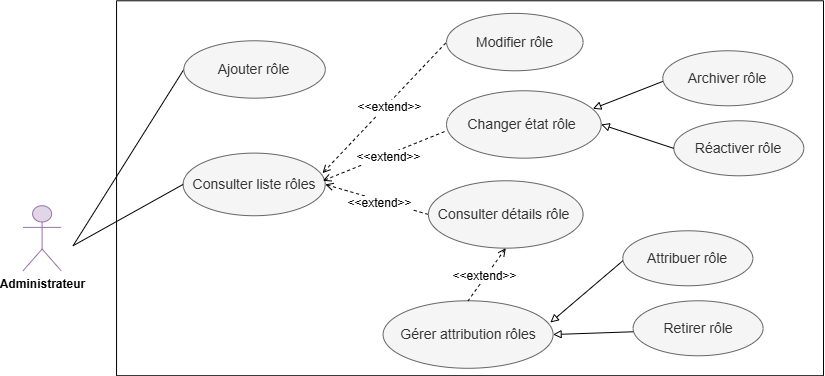
\includegraphics[width=0.8\textwidth,keepaspectratio]{Images/diag cas d'utilisation role.drawio.png}
\caption{Raffinement de cas d'utilisation « Gérer rôles »}
\label{fig:gerer_roles}
\end{figure}

\subsubsection{Description textuelle de cas d'utilisation « Archiver rôle »}

\footnotesize
\renewcommand{\arraystretch}{0.95}
\begin{longtable}{|P{3.5cm}|P{10.5cm}|}
\caption{Description textuelle « Archiver rôle »} \\
\hline
\endfirsthead
\hline
\endhead
\hline
\endfoot
\hline
\endlastfoot
\textbf{Nom du cas d'utilisation} & Archiver rôle \\
\hline
\textbf{Acteurs} & Administrateur \\
\hline
\textbf{Préconditions} & L'utilisateur est authentifié\newline L'utilisateur possède la permission d'archiver les rôles\newline Le rôle ne doit pas être assigné à des utilisateurs \\
\hline
\textbf{Postconditions} & Le rôle est archivé \\
\hline
\textbf{Scénario principal} &
\begin{minipage}[t]{\linewidth}\raggedright
\begin{enumerate}[label=\arabic*., leftmargin=0.6cm, nosep, itemsep=1pt]
\item L'administrateur sélectionne un rôle dans la liste.
\item L'administrateur clique sur l'action (Archiver).
\item Le système vérifie que le rôle n'est pas assigné à des utilisateurs.
\item Le système affiche une confirmation.
\item L'administrateur confirme l'action.
\item Le système marque le rôle comme archivé.
\item Le système affiche le message de succès.
\end{enumerate}
\end{minipage} \\
\hline
\textbf{Scénarios d'exception} & Le rôle est encore assigné à des utilisateurs. \\
\hline
\textbf{Scénarios alternatifs} & L'administrateur restaure un rôle archivé. \\
\hline
\end{longtable}
\normalsize
\vspace{-0.3cm}

\subsubsection{Description textuelle de cas d'utilisation « Attribuer rôle à utilisateur »}

\footnotesize
\renewcommand{\arraystretch}{0.95}
\needspace{10\baselineskip}
\begin{longtable}{|P{3.5cm}|P{10.5cm}|}
\caption{Description textuelle « Attribuer rôle à utilisateur »} \\
\hline
\endfirsthead
\hline
\endhead
\hline
\endfoot
\hline
\endlastfoot
\textbf{Nom du cas d'utilisation} & Attribuer rôle à utilisateur \\
\hline
\textbf{Acteurs} & Administrateur \\
\hline
\textbf{Préconditions} & L'utilisateur est authentifié\newline L'utilisateur possède la permission d'attribuer des rôles\newline Utilisateur et rôle existent \\
\hline
\textbf{Postconditions} & Le rôle est attribué à l'utilisateur \\
\hline
\textbf{Scénario principal} &
\begin{minipage}[t]{\linewidth}\raggedright
\begin{enumerate}[label=\arabic*., leftmargin=0.6cm, nosep, itemsep=1pt]
\item L'administrateur consulte le profil d'un utilisateur.
\item L'administrateur clique sur "Ajouter un rôle".
\item Le système affiche la liste des rôles disponibles.
\item L'administrateur sélectionne un rôle.
\item L'administrateur valide la sélection.
\item Le système vérifie les règles d'exclusivité métier :
  \begin{itemize}[nosep,label=$-$]
    \item Un utilisateur ayant le rôle \texttt{CLIENT} ne peut pas recevoir les rôles \texttt{CHEF\_PROJET} ou \texttt{DEVELOPPEUR}.
    \item Un utilisateur ayant le rôle \texttt{CLIENT} ne peut pas recevoir le rôle \texttt{ADMIN}.
    \item La combinaison \texttt{ADMIN} + \texttt{CHEF\_PROJET} est \textbf{autorisée}.
  \end{itemize}
\item Le système crée l'attribution.
\item Le système affiche le message de succès.
\end{enumerate}
\end{minipage} \\
\hline
\textbf{Scénarios alternatifs} & L'administrateur peut aussi attribuer le rôle depuis les détails du rôle en sélectionnant un ou plusieurs utilisateurs à qui l'attribuer. \\
\hline
\textbf{Scénarios d'exception} &
\begin{itemize}[nosep,leftmargin=0.6cm,topsep=0pt,itemsep=1pt, label=$\bullet$]
\item Le rôle est déjà attribué à cet utilisateur.
\item Violation des règles d'exclusivité des rôles.
\end{itemize} \\
\hline
\end{longtable}
\normalsize
\vspace{-0.3cm}

\subsubsection{Description textuelle de cas d'utilisation « Retirer rôle utilisateur »}

\footnotesize
\renewcommand{\arraystretch}{0.95}
\begin{longtable}{|P{3.5cm}|P{10.5cm}|}
\caption{Description textuelle « Retirer rôle utilisateur »} \\
\hline
\endfirsthead
\hline
\endhead
\hline
\endfoot
\hline
\endlastfoot
\textbf{Nom du cas d'utilisation} & Retirer rôle utilisateur \\
\hline
\textbf{Acteurs} & Administrateur \\
\hline
\textbf{Préconditions} & L'utilisateur est authentifié\newline L'utilisateur possède la permission de retirer des rôles\newline Le rôle est attribué à l'utilisateur \\
\hline
\textbf{Postconditions} & Le rôle est retiré de l'utilisateur \\
\hline
\textbf{Scénario principal} &
\begin{minipage}[t]{\linewidth}\raggedright
\begin{enumerate}[label=\arabic*., leftmargin=0.6cm, nosep, itemsep=1pt]
\item L'administrateur consulte le profil d'un utilisateur.
\item L'administrateur visualise les rôles actuels de l'utilisateur.
\item L'administrateur clique sur l'icône de suppression d'un rôle.
\item Le système affiche une confirmation.
\item L'administrateur confirme l'action.
\item Le système retire le rôle.
\item Le système affiche le message de succès.
\end{enumerate}
\end{minipage} \\
\hline
\textbf{Scénarios d'exception} &
\begin{itemize}[nosep,leftmargin=0.6cm,topsep=0pt,itemsep=1pt, label=$\bullet$]
\item L'administrateur tente de retirer le dernier rôle de l'utilisateur.
\item Le rôle n'est pas attribué à cet utilisateur.
\end{itemize} \\
\hline
\end{longtable}
\normalsize
\vspace{-0.3cm}

\subsection{Analyse de la fonctionnalité « Gérer permissions »}
Dans cette partie, nous allons présenter les cas d'utilisation relatifs à la gestion des permissions afin
de comprendre les principales fonctionnalités du système, ce qui permet d'avoir une vue globale des
interactions.
\subsubsection{Raffinement de cas d'utilisation « Gérer permissions »}
Au cours de cette partie, nous allons analyser chaque cas d'utilisation raffiné pour le cas de gestion des permissions :

\begin{figure}[htbp]
\centering
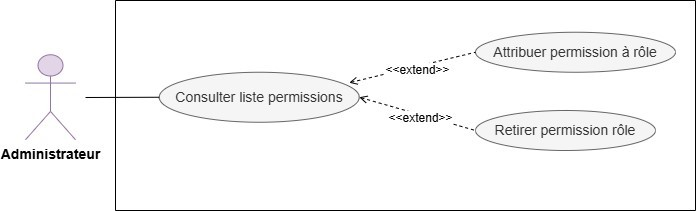
\includegraphics[width=0.8\textwidth,keepaspectratio]{Images/gerer permession.drawio.jpg}
\caption{Raffinement de cas d'utilisation « Gérer permissions »}
\label{fig:gerer_permissions}
\end{figure}

\subsubsection{Description textuelle de cas d'utilisation « Consulter liste permissions »}

\footnotesize
\renewcommand{\arraystretch}{0.95}
{\sloppy
\begin{longtable}{|P{3.5cm}|P{10.5cm}|}
\caption{Description textuelle « Consulter liste permissions »} \\
\hline
\endfirsthead
\hline
\endhead
\hline
\endfoot
\hline
\endlastfoot
\textbf{Nom du cas d'utilisation} & Consulter liste des permissions \\
\hline
\textbf{Acteurs} & Administrateur \\
\hline
\textbf{Préconditions} & L'utilisateur est authentifié\newline L'utilisateur possède la permission de consulter les permissions \\
\hline
\textbf{Postconditions} & Liste des permissions affichée \\
\hline
\textbf{Scénario principal} &
\begin{minipage}[t]{\linewidth}\raggedright
\begin{enumerate}[label=\arabic*., leftmargin=0.6cm, nosep, itemsep=1pt]
\item L'administrateur accède à la section "Permissions".
\item Le système affiche une matrice avec les rôles en horizontal et les catégories de permissions en vertical.
\item L'administrateur peut visualiser quelles permissions sont attribuées à chaque rôle (cases cochées).
\item L'administrateur peut filtrer par catégorie de permissions ou par rôle.
\end{enumerate}
\end{minipage} \\
\hline
\textbf{Scénarios alternatifs} &
\begin{itemize}[nosep,leftmargin=0.6cm,topsep=0pt,itemsep=1pt, label=$\bullet$]
\item L'administrateur sélectionne la vue "Par rôle" pour afficher une liste des rôles avec leurs permissions respectives organisées par catégorie.
\item L'administrateur clique sur le bouton « Exporter » pour télécharger la matrice des permissions.
\end{itemize} \\
\hline
\end{longtable}
}
\normalsize
\vspace{-0.3cm}

\subsubsection{Description textuelle de cas d'utilisation « Attribuer permission à rôle »}

\footnotesize
\renewcommand{\arraystretch}{0.95}
{\sloppy
\begin{longtable}{|P{3.5cm}|P{10.5cm}|}
\caption{Description textuelle « Attribuer permission à rôle »} \\
\hline
\endfirsthead
\hline
\endhead
\hline
\endfoot
\hline
\endlastfoot
\textbf{Nom du cas d'utilisation} & Attribuer permission à rôle \\
\hline
\textbf{Acteurs} & Administrateur \\
\hline
\textbf{Préconditions} & L'utilisateur est authentifié\newline L'utilisateur possède la permission d'attribuer des permissions aux rôles\newline Rôle et permission existent \\
\hline
\textbf{Postconditions} & La permission est ajoutée au rôle \\
\hline
\textbf{Scénario principal} &
\begin{minipage}[t]{\linewidth}\raggedright
\begin{enumerate}[label=\arabic*., leftmargin=0.6cm, nosep, itemsep=1pt]
\item L'administrateur consulte un rôle spécifique.
\item L'administrateur clique sur l'onglet "Permissions".
\item Le système affiche toutes les permissions organisées par catégorie avec des cases à cocher.
\item L'administrateur coche les permissions à attribuer.
\item L'administrateur clique sur "Enregistrer".
\item Le système crée les liaisons.
\item Le système affiche le message de succès.
\end{enumerate}
\end{minipage} \\
\hline
\textbf{Scénarios alternatifs} & L'administrateur utilise la matrice des permissions pour cocher les cases correspondant aux permissions à attribuer pour plusieurs rôles simultanément. \\
\hline
\textbf{Scénarios d'exception} & La permission est déjà attribuée au rôle. \\
\hline
\end{longtable}
}
\normalsize
\vspace{-0.3cm}

% ─────────────────────────────────────────────────────────────────────────────
% SECTION 3 : CONCEPTION
% ─────────────────────────────────────────────────────────────────────────────

\section{Diagramme de classes de premiére sprint}

\begin{figure}[htbp]
        \centering
        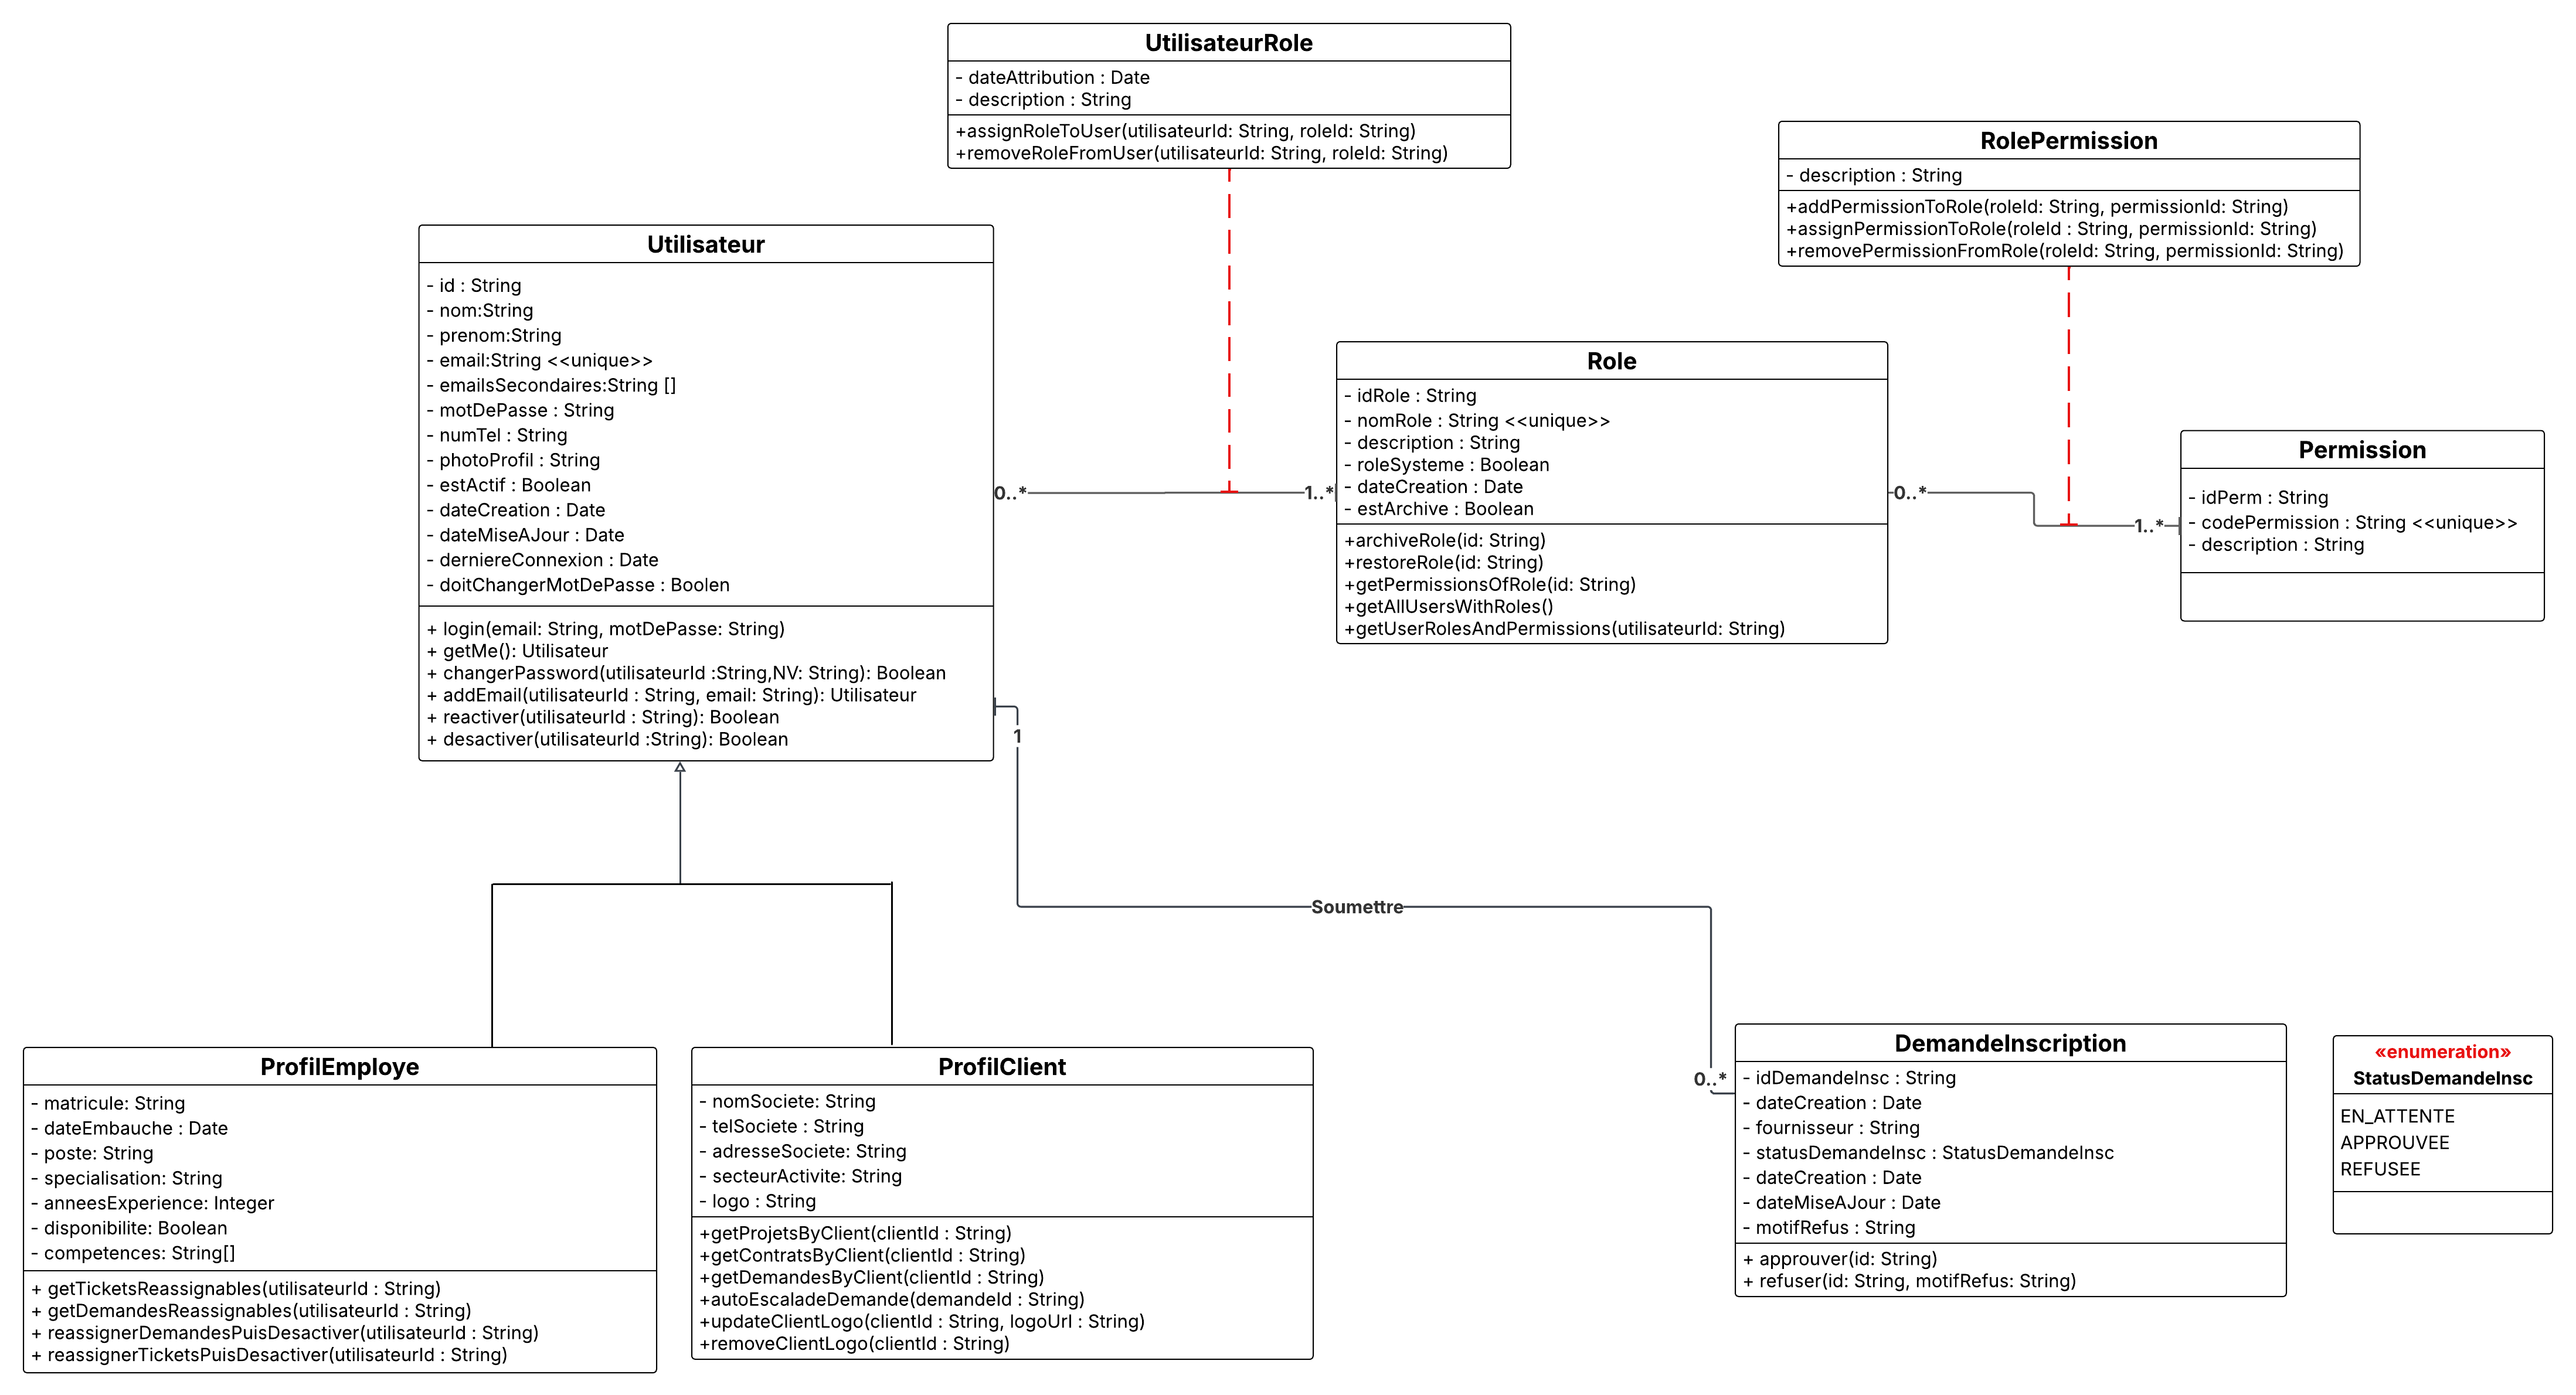
\includegraphics[width=1\textwidth,keepaspectratio]{Images/diag classe sprint 1.png}
        \caption{Diagramme de classes du Sprint 1}
        \label{fig:diag_classe_sprint1}
\end{figure}

\section{Diagramme de séquence}

\subsection{Diagramme de séquences du cas d'utilisation « S'authentifier »}

\begin{figure}[H]
        \centering
        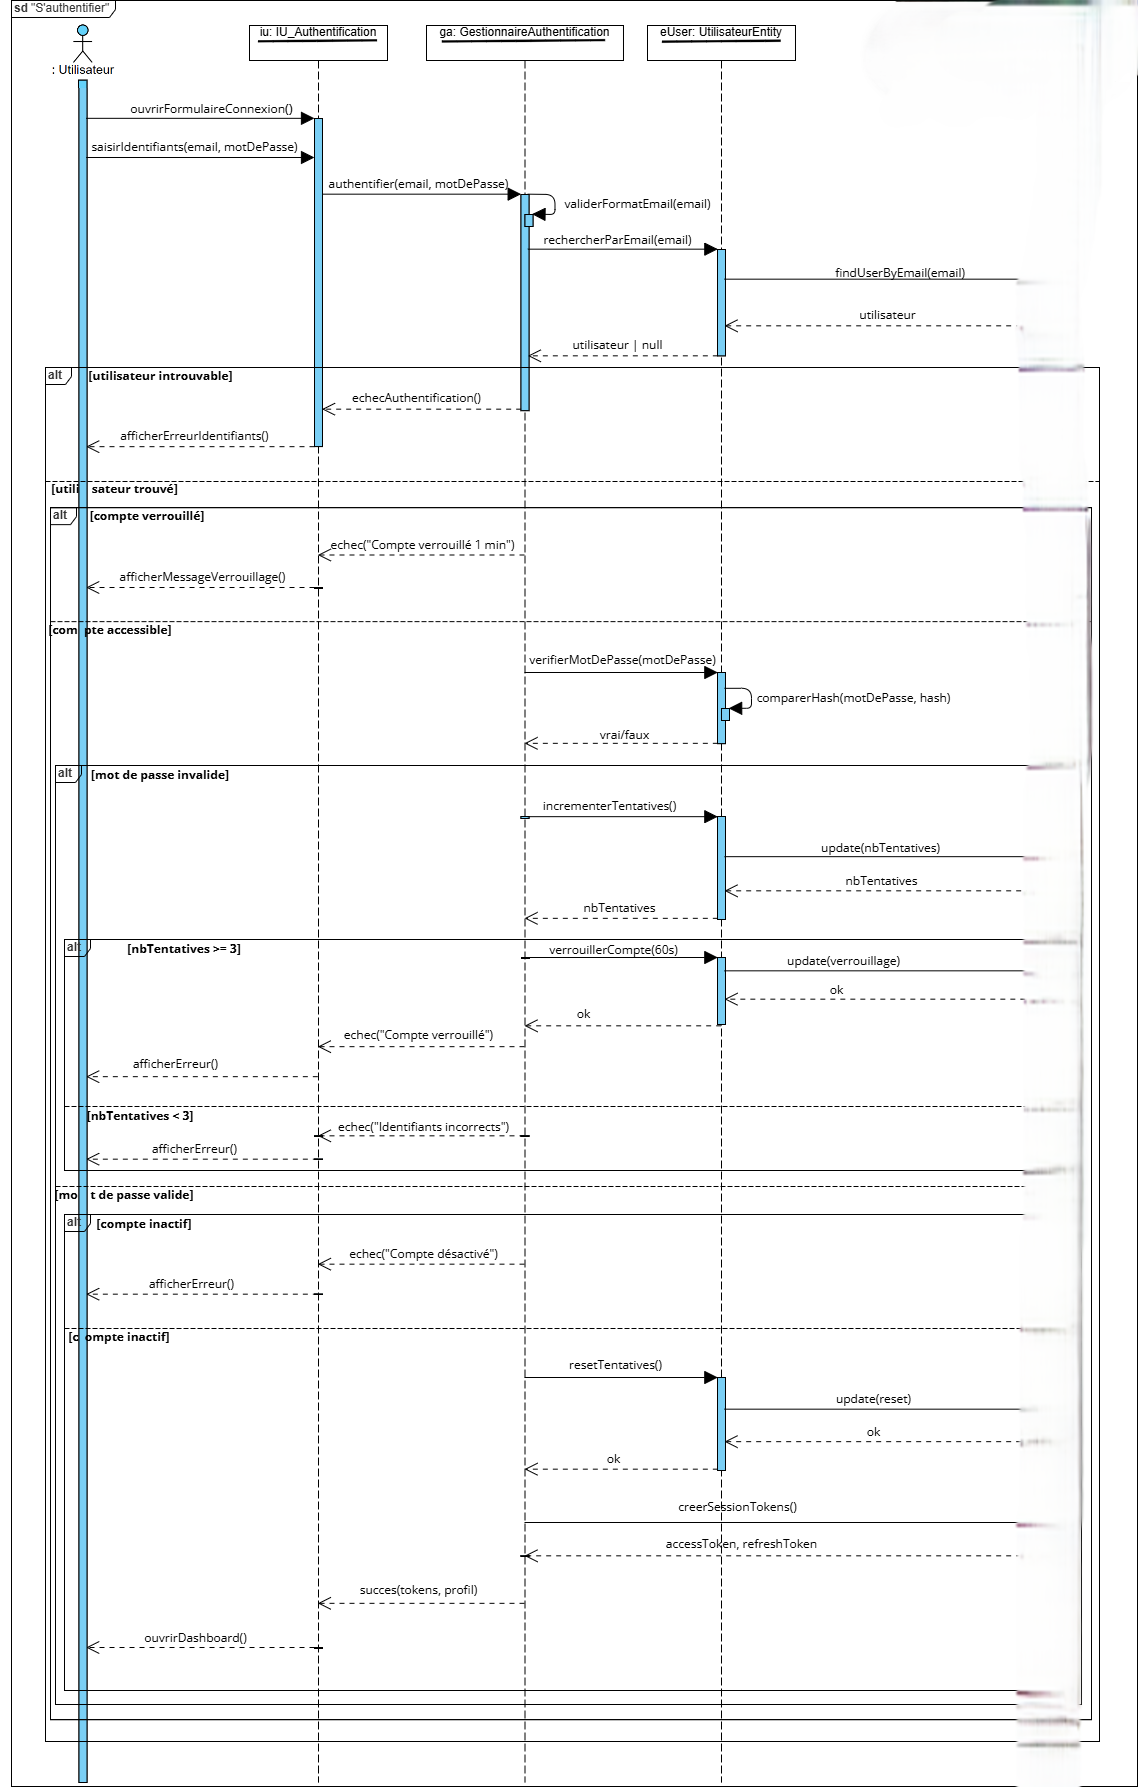
\includegraphics[width=0.7\textwidth,keepaspectratio]{Images/diag_seq_auth.png}
        \caption{Diagramme de séquence du cas d'utilisation « S'authentifier »}
        \label{fig:auth_sequence}
\end{figure}

\subsection{Diagramme de séquences du cas d'utilisation « Mot de passe oublié »}

\begin{figure}[H]
        \centering
        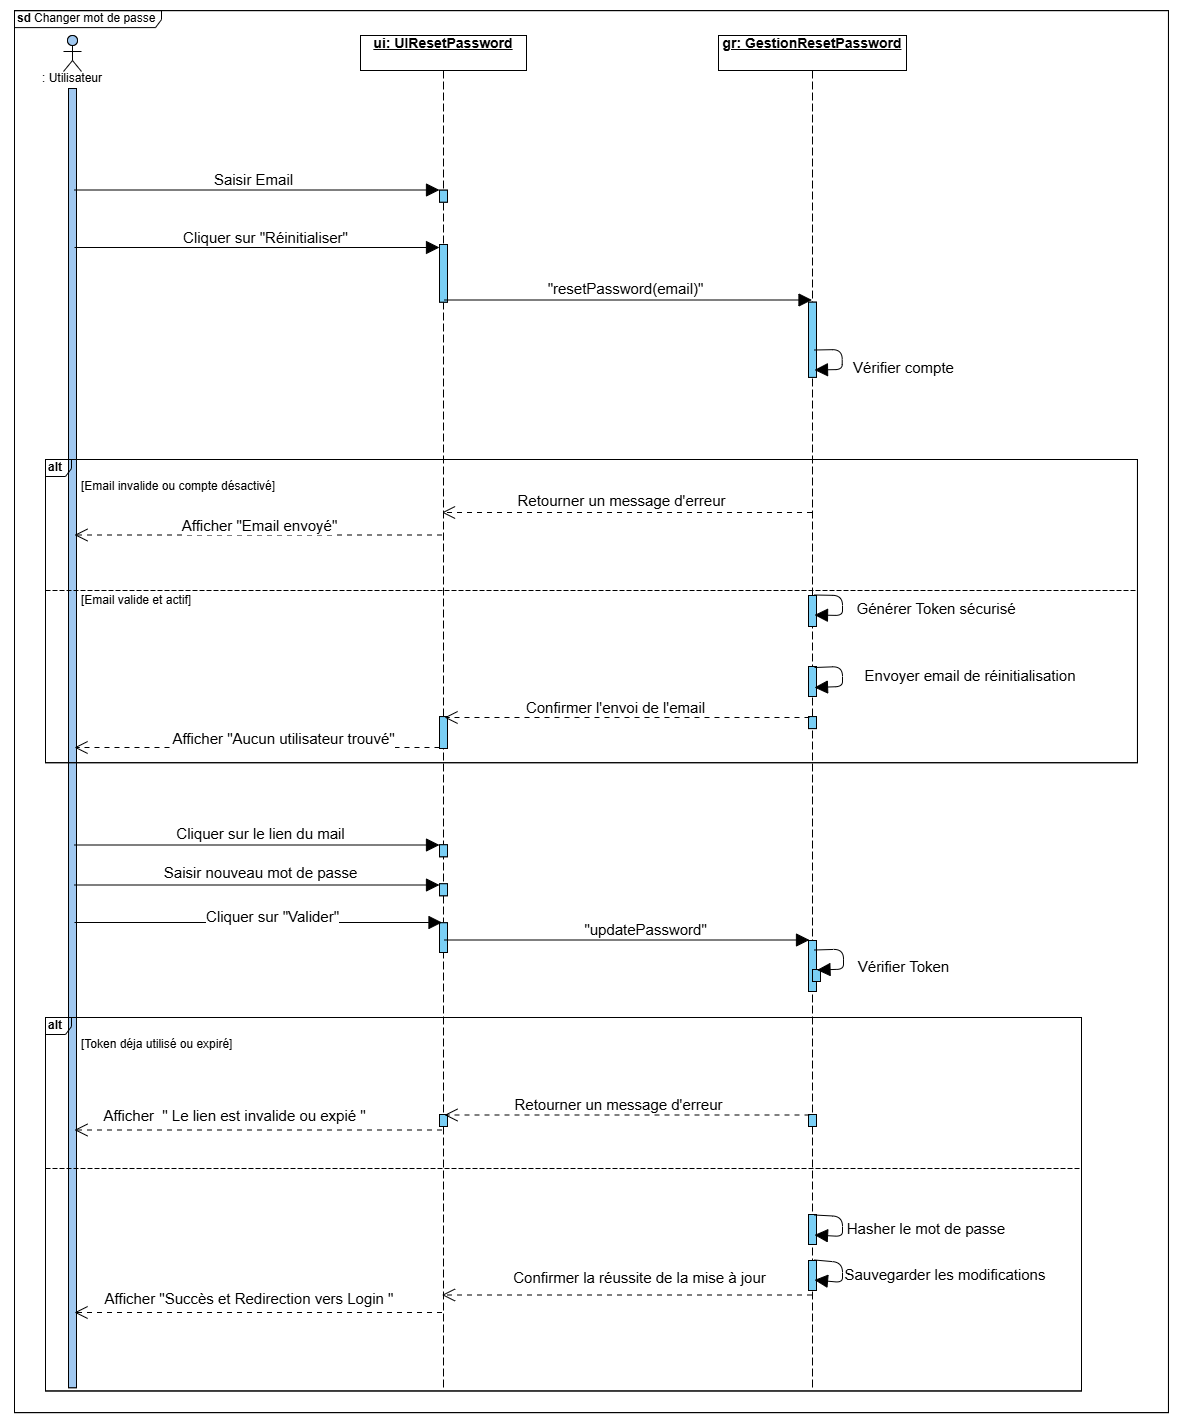
\includegraphics[width=0.7\textwidth,keepaspectratio]{Images/Diagramme changer Mot de passe.png}
        \caption{Diagramme de séquence du cas d'utilisation « Mot de passe oublié »}
        \label{fig:password_reset_sequence}
\end{figure}

\subsection{Diagramme de séquences du cas d'utilisation « Désactiver utilisateur »}

\begin{figure}[H]
        \centering
        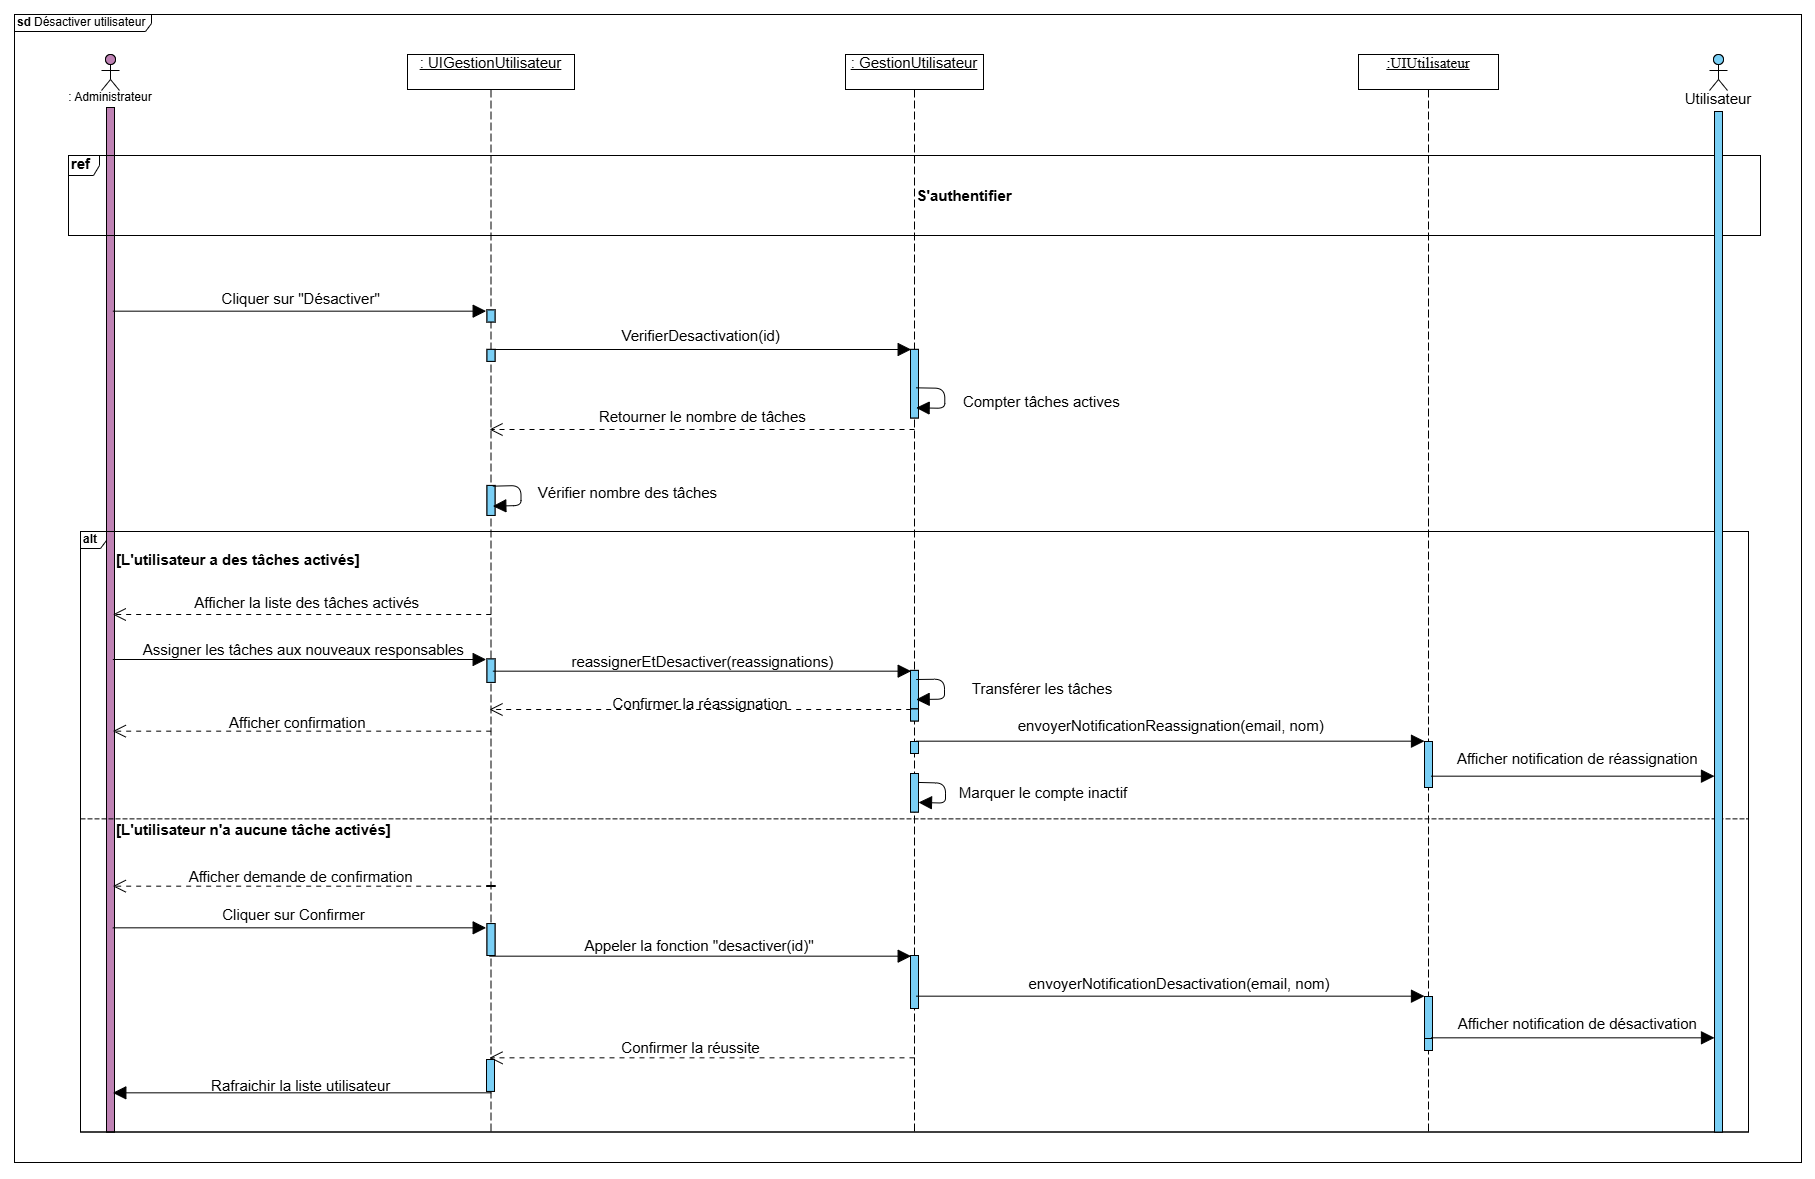
\includegraphics[width=0.7\textwidth,keepaspectratio]{Images/Diaggramme de séquence de Désactiver utilisateur.png}
        \caption{Diagramme de séquence du cas d'utilisation « Désactiver utilisateur »}
        \label{fig:deactivate_user_sequence}
\end{figure}

\subsection{Diagramme d'activité « Authentification et Demander accés via fournisseur externe »}

\begin{figure}[htbp]
        \centering
        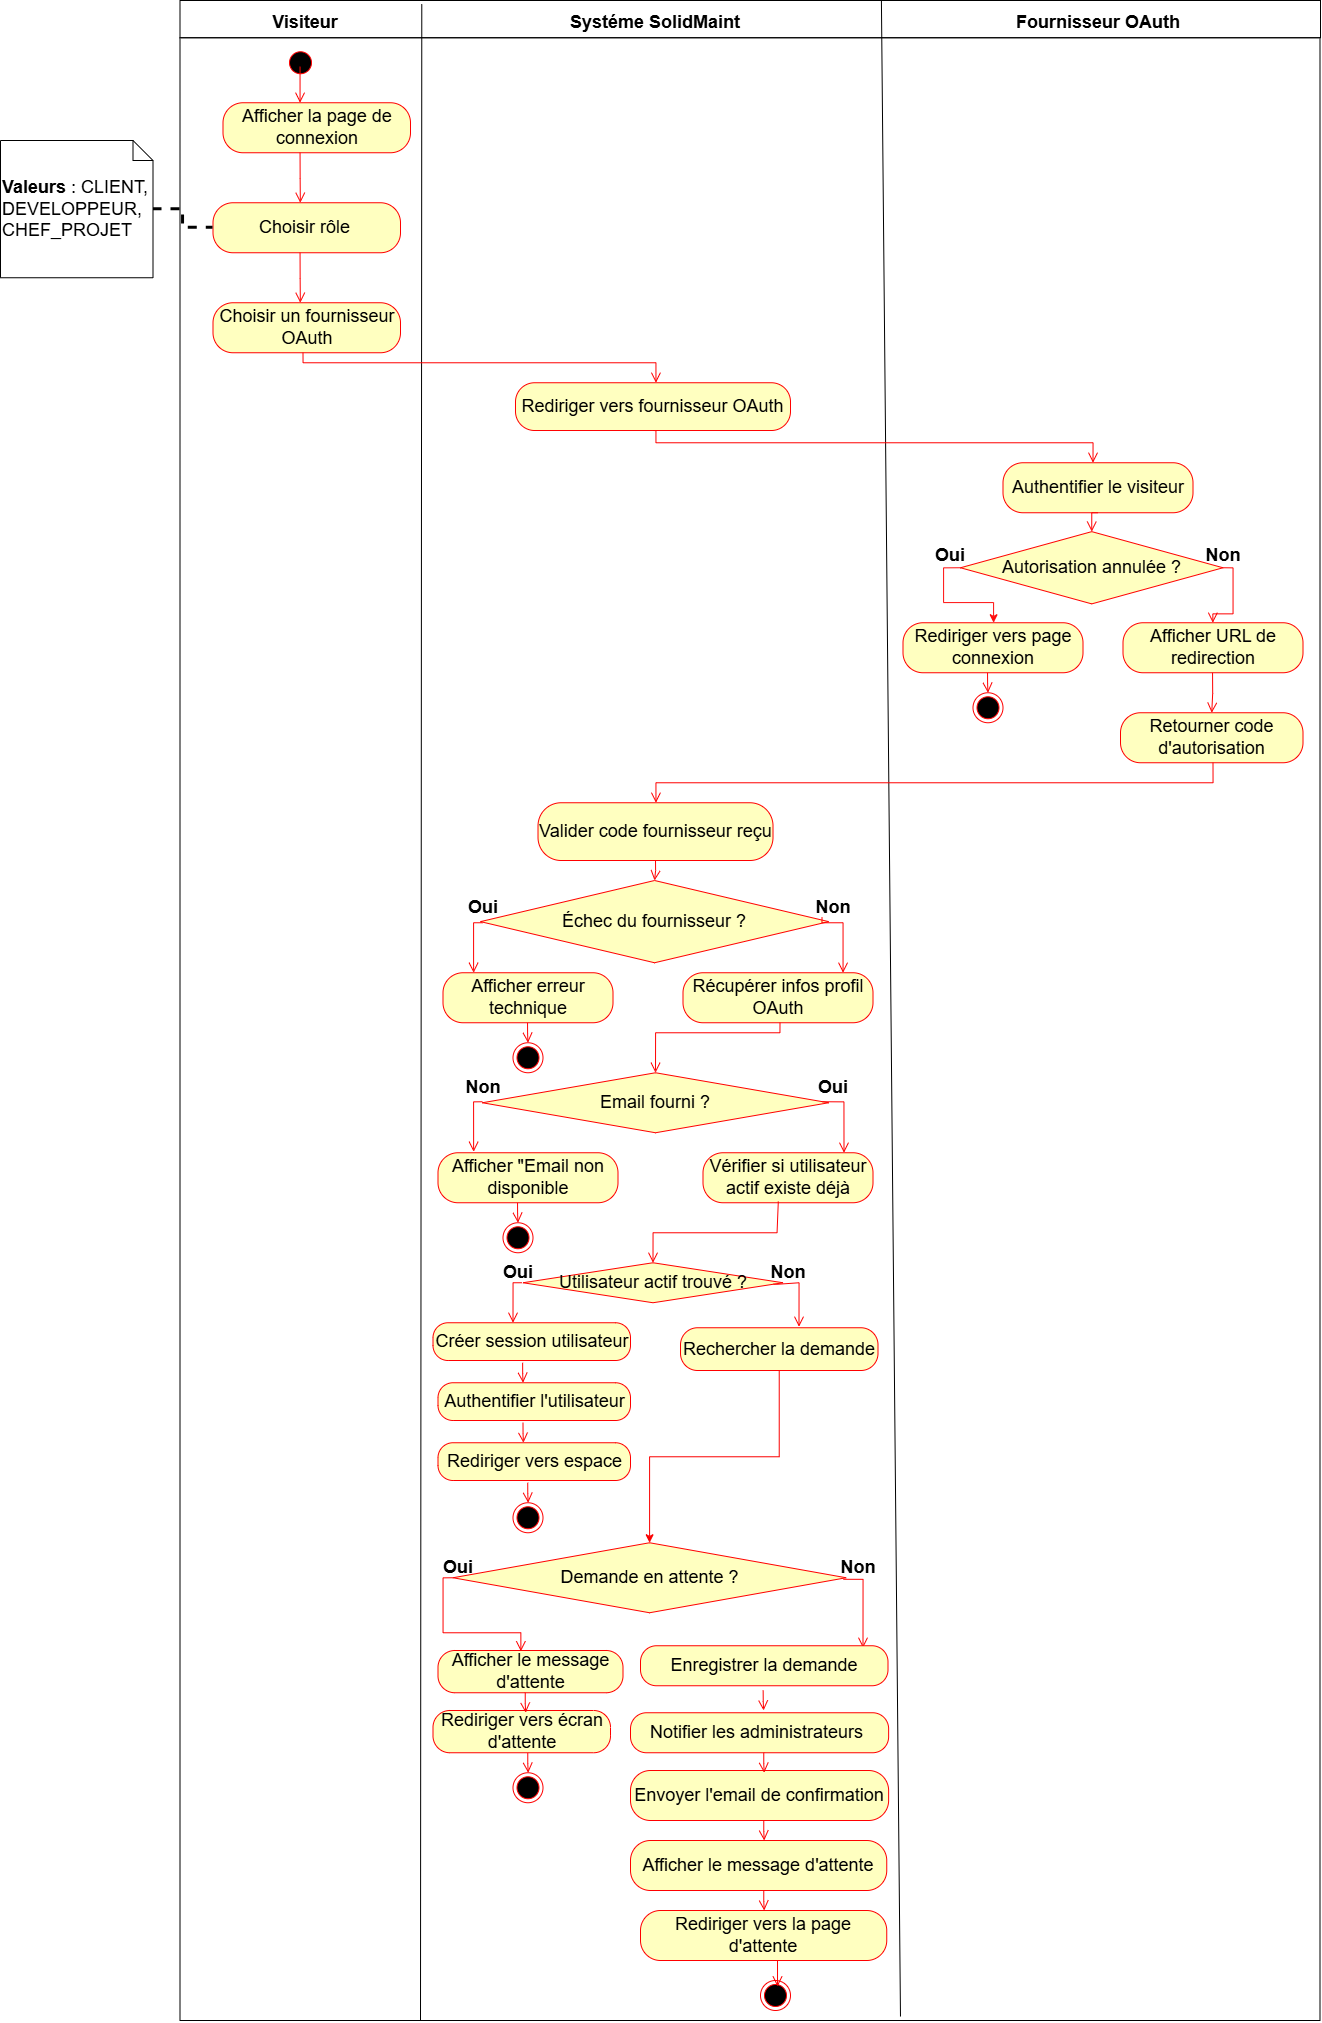
\includegraphics[width=0.9\textwidth,keepaspectratio]{Images/diag_activites_demande_insc.png}
        \caption{Diagramme d'activité d'authentification et Demande accés via fournisseur externe}
        \label{fig:oauth_activity_diagram}
\end{figure}

\section{Schéma relationnel}

\textbf{Utilisateur} (\underline{idUtilisateur}, nom, prenom, email,
  motDePasse, estActif, doitChangerMotDePasse, tentativesConnexionEchouees,
  compteVerrouilleJusquA, photoProfil, dateCreation)
\newline
\textbf{ProfilEmploye} (\underline{idProfilE}, \textbf{\#idUtilisateur},
  matricule, poste, specialisation, disponibilite, dateEmbauche,
  niveauSeniorite)
\newline
\textbf{ProfilClient} (\underline{idProfilC}, \textbf{\#idUtilisateur},
  nomSociete, adresseSociete, secteurActivite, telSociete, logo)
\newline
\textbf{Role} (\underline{idRole}, nomRole, description, roleSysteme,
  estArchive, dateCreation)
\newline
\textbf{Permission} (\underline{idPermission}, codePermission, description)
\newline
\textbf{UtilisateurRole} (\underline{idUtilisateurRole},
  \textbf{\#idUtilisateur}, \textbf{\#idRole}, dateAttribution)
\newline
\textbf{RolePermission} (\underline{idRolePermission}, \textbf{\#idRole},
  \textbf{\#idPermission})
\newline
\textbf{DemandeInscriptionOAuth} (\underline{idDemande}, email, prenom, nom,
  fournisseur, photoProfil, role, statut, dateCreation, motifRefus)
% ─────────────────────────────────────────────────────────────────────────────
% SECTION 4 : RÉALISATION
% ─────────────────────────────────────────────────────────────────────────────

\section{Réalisation}
Après avoir analysé les besoins et conçu les solutions, nous passons maintenant à la réalisation. Dans cette phase, nous avons développé toutes les user stories planifiées dans le sprint backlog. Cette section présente le diagramme de composants qui montre l'architecture de notre application, ainsi que les interfaces utilisateur que nous avons créées pour répondre aux besoins des utilisateurs.
\label{sec:realisation_sprint1}

\subsection{Diagramme de composants}


\subsection{Description des interfaces}
Cette section présente les principales interfaces utilisateur développées lors du premier sprint.

\subsubsection{Interface de connexion}
\begin{figure}[H]
\centering
%\includegraphics[width=0.75\textwidth,keepaspectratio]{Images/interface_connexion.png}
\caption{Interface de connexion — authentification classique et OAuth}
\label{fig:interface_connexion}
\end{figure}
La page de connexion propose deux modes d'authentification : le formulaire
classique (e-mail + mot de passe) et les boutons OAuth (Google, GitHub).
En cas de compte inexistant, le visiteur est redirigé vers un flux de
demande d'inscription.

\subsubsection{Interface de réinitialisation du mot de passe}
\begin{figure}[H]
\centering
%\includegraphics[width=0.75\textwidth,keepaspectratio]{Images/interface_reset_password.png}
\caption{Interface de réinitialisation du mot de passe}
\label{fig:interface_reset}
\end{figure}
Cette interface permet à l'utilisateur de saisir son adresse e-mail pour
recevoir un lien de réinitialisation valable 1 heure.

\subsubsection{Interface de gestion des utilisateurs}
\begin{figure}[H]
\centering
%\includegraphics[width=0.85\textwidth,keepaspectratio]{Images/interface_users.png}
\caption{Interface d'administration — liste des utilisateurs}
\label{fig:interface_users}
\end{figure}
L'administrateur dispose d'une vue en grille ou en liste, avec filtres par
statut et par rôle, barre de recherche et actions rapides (modifier,
désactiver, voir le profil).

\subsubsection{Interface de gestion des rôles et permissions}
\begin{figure}[H]
\centering
%\includegraphics[width=0.85\textwidth,keepaspectratio]{Images/interface_roles_permissions.png}
\caption{Interface d'administration — gestion des rôles et permissions}
\label{fig:interface_roles}
\end{figure}
La matrice des permissions affiche les rôles en colonnes et les catégories
de permissions en lignes, avec des cases à cocher pour une attribution
visuelle et intuitive.

\subsubsection{Interface de gestion des Demandes d'accès via fournisseur externe}
\begin{figure}[H]
\centering
%\includegraphics[width=0.85\textwidth,keepaspectratio]{Images/interface_demandes_oauth.png}
\caption{Interface d'administration — demandes d'inscription OAuth}
\label{fig:interface_oauth}
\end{figure}
L'administrateur consulte les demandes en attente, visualise les
informations récupérées via OAuth et peut approuver ou refuser chaque
demande avec un motif de refus facultatif.

% ─────────────────────────────────────────────────────────────────────────────
% SECTION 5 : TESTS
% ─────────────────────────────────────────────────────────────────────────────
\section{Tests et Validation}
La phase de test est essentielle pour garantir la qualité et la fiabilité de la solution. Elle valide que chaque fonctionnalité répond aux exigences métier et identifie les anomalies avant la mise en production. Dans ce sprint, nous avons testé les mécanismes d'authentification, la gestion des utilisateurs et le contrôle d'accès (RBAC) pour assurer la robustesse de nos implémentations.

\subsection{Stratégie de tests adoptée}
Afin de garantir la qualité et la fiabilité de l'application, nous avons adopté une stratégie de tests structurée, reposant sur une répartition des vérifications à plusieurs niveaux. Cette approche permet d'assurer une bonne couverture fonctionnelle avec un temps d'exécution raisonnable, tout en facilitant l'identification rapide des anomalies.

Les tests ont été organisés par module fonctionnel afin d'assurer une meilleure traçabilité des vérifications effectuées. Ainsi, les tests unitaires couvrent les règles métier les plus fines, les tests d'intégration valident les échanges avec l'API, et les tests End-to-End reproduisent les scénarios complets d'utilisation de l'application.

La pyramide de tests se compose donc de trois niveaux complémentaires :


\subsubsection{Tests unitaires}
\label{sec:tests_unitaires}

Les tests unitaires ont été réalisés à l'aide du framework \textbf{Vitest},
en isolant chaque service du reste de l'application grâce à des mocks
Prisma. Cette approche garantit l'indépendance des tests et permet une
détection précoce des anomalies dès la phase de développement. Trois
modules prioritaires ont été couverts : l'authentification, le contrôle
d'accès basé sur les rôles (RBAC) et la gestion des clients.


\noindent\textbf{Bilan : 45 tests exécutés — 45 réussis — 0 échec.}
\vspace{6pt}

\begin{itemize}[leftmargin=0pt]

% ── 1. Authentification ───────────────────────────────────────────────────────
\item[$\square$] \textbf{Module Authentification}
\newline
\newline
\textit{Méthodes : \texttt{login()} ·
\texttt{demanderReinitialisationMotDePasse()} ·
\texttt{reinitialiserMotDePasse()}}

\noindent Cette suite valide le processus d'authentification classique,
la génération des jetons JWT et le mécanisme de réinitialisation du mot
de passe. Les cas suivants ont été couverts :

\begin{itemize}[label=$\bullet$, nosep, itemsep=2pt]
  \item Un utilisateur actif fournit des identifiants valides : les jetons
    \texttt{accessToken} et \texttt{refreshToken} sont générés
    correctement.
  \item L'adresse e-mail fournie n'existe pas en base de données : la
    connexion est rejetée avec le code \texttt{401 Unauthorized}.
  \item Le mot de passe fourni est incorrect : la connexion est rejetée
    avec le code \texttt{401 Unauthorized}.
  \item L'utilisateur échoue l'authentification \textbf{3 fois
    consécutives} : le compte est verrouillé automatiquement pendant
    \textbf{1 minute} (\texttt{maxLoginAttempts = 3}).
  \item L'utilisateur tente de se connecter alors que son compte est
    verrouillé : la connexion est rejetée avec un message explicite.
  \item Le compte de l'utilisateur est désactivé : la connexion est
    rejetée avec le code \texttt{401 Unauthorized}.
  \item L'adresse e-mail fournie pour la réinitialisation est inexistante :
    une \texttt{NotFoundException} est levée.
  \item Le token de réinitialisation a été généré depuis plus d'une heure :
    une \texttt{BadRequestException} est levée.
\end{itemize}
\begin{figure}[htbp]
\centering
\begin{minipage}{0.48\textwidth}
  \centering
  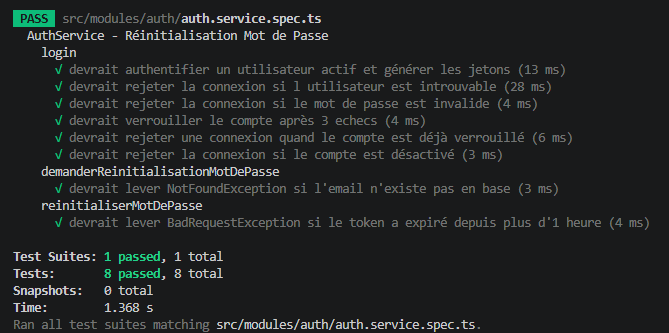
\includegraphics[width=\textwidth,keepaspectratio]
    {Images/test-unitaire-auth.png}
  \caption*{\small Auth}
\end{minipage}
\end{figure}
% ── 2. RBAC ───────────────────────────────────────────────────────────────────
\item[$\square$] \textbf{Module Gestion des rôles et permissions (RBAC)}
\newline
\textit{Méthodes :} \texttt{creerPermission()},
\texttt{attribuerRoleUtilisateur()},
\texttt{obtenirRolesEtPermissions()}
\noindent Cette suite valide les règles d'exclusivité des rôles, l'unicité
des permissions et l'intégrité des références.
\newline
Les cas suivants ont été couverts :

\begin{itemize}[label=$\bullet$, nosep, itemsep=2pt]
  \item Une permission est créée avec un code unique : elle est enregistrée
    correctement en base de données.
  \item Une permission est créée avec un code déjà existant : une
    \texttt{BadRequestException} est levée.
  \item Les rôles et permissions d'un utilisateur sont récupérés : la liste
    est retournée sans doublons.
  \item Un rôle est attribué à un utilisateur sans rôle existant :
    l'attribution est réussie.
  \item L'utilisateur cible est inexistant : une \texttt{NotFoundException}
    est levée.
  \item La règle d'exclusivité \texttt{CLIENT} et \texttt{CHEF\_PROJET}
    est violée : une \texttt{BadRequestException} est levée.
  \item La règle d'exclusivité \texttt{CLIENT} et \texttt{DEVELOPPEUR}
    est violée : une \texttt{BadRequestException} est levée.
  \item La règle d'exclusivité \texttt{CLIENT} et \texttt{ADMIN} est
    violée : une \texttt{BadRequestException} est levée.
  \item La combinaison \texttt{ADMIN} et \texttt{CHEF\_PROJET} est
    soumise : l'attribution est \textbf{autorisée} et réussie.
  \item Le rôle est déjà attribué à l'utilisateur : une
    \texttt{BadRequestException} est levée (doublon détecté).
  \item Le rôle à attribuer est inexistant : une \texttt{NotFoundException}
    est levée.
\end{itemize}
\begin{figure}[htbp]
   \centering
\begin{minipage}{0.48\textwidth}
  \centering
  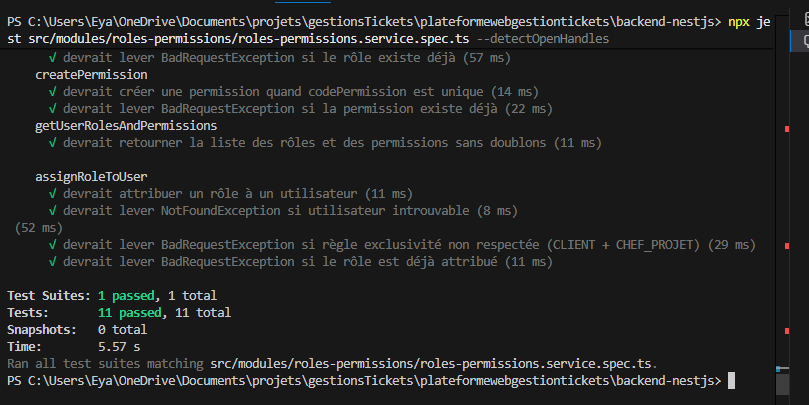
\includegraphics[width=\textwidth,keepaspectratio]{Images/test-sprint1-moduleRole+Permession.png}
  \caption*{\small RBAC}
\end{minipage}
\caption{Résultats des tests unitaires — Auth et RBAC}
\label{fig:test_unitaires}
\end{figure}
% ── 3. Gestion des clients ────────────────────────────────────────────────────

\end{itemize}

\subsubsection{Tests d'intégration}
\label{sec:tests_integration}

Les tests d'intégration ont pour objectif de valider les échanges entre
les différentes couches de l'application (contrôleur, service et base de
données) en testant les endpoints REST dans leur ensemble. Ces tests sont
effectués via \textbf{Swagger UI} en soumettant des requêtes HTTP réelles
contre le backend en cours d'exécution, ce qui permet de vérifier le
comportement de l'API dans des conditions proches de la production.

\begin{itemize}[leftmargin=0pt]

\item[$\square$] \textbf{Authentification}
 \newline
\newline\textit{Endpoint : \texttt{POST /api/auth/login}}

\noindent Cette suite valide le comportement complet de l'endpoint de
connexion, notamment le retour des jetons d'authentification, des rôles,
des permissions associées et la gestion des codes d'erreur HTTP selon les
différents cas d'entrée.
\newline Les cas suivants ont été couverts :

\begin{itemize}[label=$\bullet$, nosep, itemsep=2pt]
  \item Un utilisateur actif de rôle \texttt{ADMIN} fournit des
    identifiants valides : l'endpoint retourne le code \textbf{200 OK}
    accompagné des champs \texttt{accessToken}, \texttt{refreshToken},
    des données de l'utilisateur, de ses rôles et de la liste complète
    de ses permissions.
  \item L'adresse e-mail fournie n'existe pas en base de données :
    l'endpoint retourne le code \textbf{401 Unauthorized}.
  \item Le mot de passe fourni est incorrect : l'endpoint retourne le
    code \textbf{401 Unauthorized}.
  \item Les données soumises sont invalides (adresse e-mail mal formatée
    ou champ obligatoire vide) : l'endpoint retourne le code
    \textbf{400 Bad Request} accompagné d'un message de validation
    généré par \texttt{class-validator}.
  \item Le compte de l'utilisateur est désactivé
    (\texttt{estActif = false}) : l'endpoint retourne le code
    \textbf{401 Unauthorized} avec le message
    « Ce compte est désactivé ».
\end{itemize}

\begin{figure}[H]
\centering
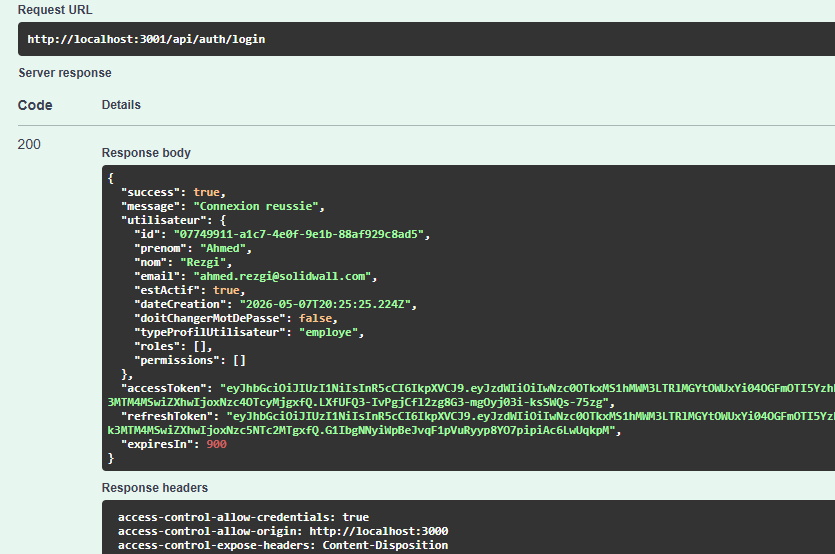
\includegraphics[width=0.60\textwidth,keepaspectratio]
  {Images/test-interg-login.png}
\caption{Test d'intégration — endpoint \texttt{POST /api/auth/login}
  via Swagger}
\label{fig:test_integration}
\end{figure}

\item[$\square$]  \textbf {Gestion du profil}
\newline
\newline\textit{Endpoint : \texttt{PUT /api/profil}}
 
\noindent Cette suite de tests vise à valider le bon fonctionnement de la méthode \textbf{modifierProfil()} exposée via l'endpoint \textbf{PUT /api/profil}, qui permet à un utilisateur de mettre à jour les informations de son profil.
\newline
Lee cas suivant ont été couvert :
\begin{itemize}
\item[$\bullet$] Cas où l'e-mail fourni dans la requête ne respecte pas le format attendu.
\end{itemize}
\begin{figure}[htbp]
        \centering
        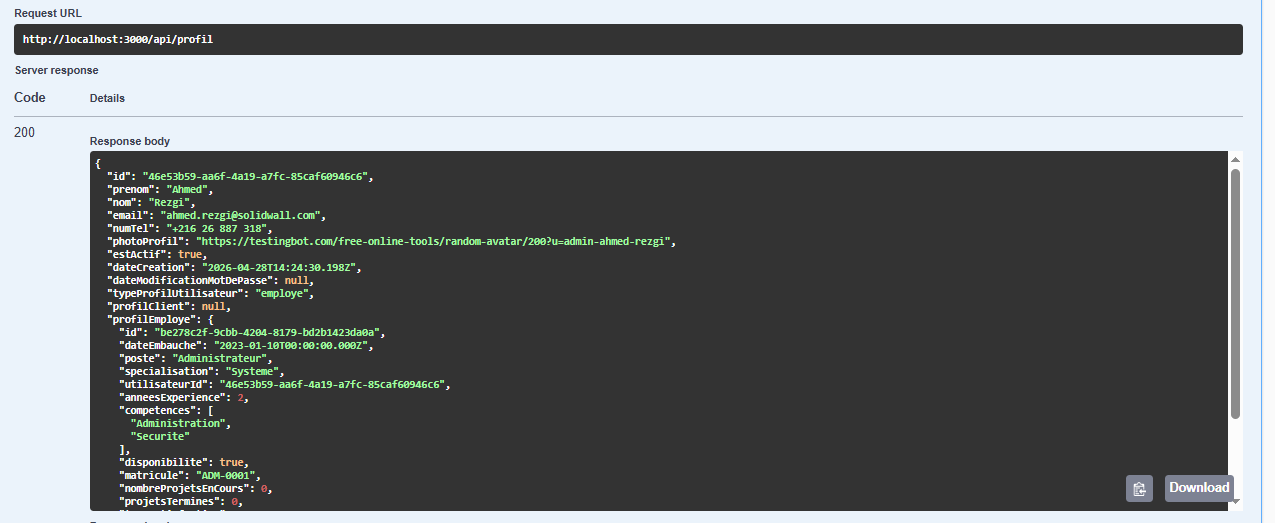
\includegraphics[width=0.7\textwidth,keepaspectratio]{Images/gestion profil Swagger.png}
        \caption{Test de mise à jour du profil}
    \end{figure}
\end{itemize}

\subsubsection{Tests End-to-End}
\label{sec:tests_e2e}

Les tests End-to-End ont pour objectif de simuler les parcours utilisateurs
complets dans un navigateur réel piloté par \textbf{Playwright}. Ces tests
s'exécutent en interaction avec le frontend Next.js, le backend NestJS et
la base de données PostgreSQL, reproduisant ainsi les conditions réelles
d'utilisation de la plateforme.
\newline

\noindent\textbf{Bilan : 11 tests exécutés — 11 réussis — 0 échec.}
\vspace{6pt}

\begin{itemize}[leftmargin=0pt]

\item[$\square$] \textbf{Authentification}
\newline
\newline\textit{10 scénarios : connexion classique, OAuth, déconnexion}

\noindent Cette suite valide le flux complet d'authentification en
simulant les actions réelles d'un utilisateur sur l'interface. Les cas
suivants ont été couverts :

\begin{itemize}[label=$\bullet$, nosep, itemsep=2pt]
  \item La page de connexion est chargée : le formulaire et les boutons
    d'authentification OAuth sont affichés correctement.
  \item Les champs du formulaire sont vides ou partiellement remplis :
    le bouton de soumission reste désactivé.
  \item L'utilisateur soumet des identifiants valides : le flux aboutit
    à une redirection vers la page d'accueil et une session est créée.
  \item L'utilisateur saisit un identifiant ou un mot de passe invalide :
    un message d'erreur approprié est affiché sans redirection.
  \item L'utilisateur échoue l'authentification \textbf{3 fois
    consécutives} : le compte est verrouillé pendant \textbf{1 minute}
    et un message d'information est affiché.
  \item L'utilisateur se déconnecte : les jetons sont supprimés du
    \texttt{localStorage} et l'utilisateur est redirigé vers la page
    \texttt{/connexion}.
  \item L'utilisateur s'authentifie via \textbf{Google} avec succès :
    les données du profil sont récupérées et une session valide est
    créée.
  \item L'authentification via \textbf{Google} échoue : un message
    d'erreur technique est affiché.
  \item L'utilisateur s'authentifie via \textbf{GitHub} avec succès :
    les données du profil sont récupérées et une session valide est
    créée.
  \item L'authentification via \textbf{GitHub} échoue : un message
    d'erreur technique est affiché.
\end{itemize}

\begin{figure}[H]
\centering
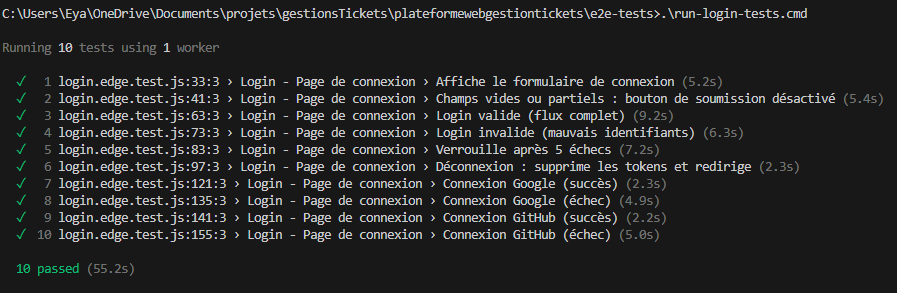
\includegraphics[width=0.68\textwidth,keepaspectratio]
  {Images/ExecDeTestCasesReussi-auth.png}
\caption{Tests End-to-End — Authentification via Playwright}
\label{fig:test_e2e_auth}
\end{figure}

\item[$\square$] \textbf{Gestion des utilisateurs} ---
\textit{1 scénario : désactivation avec réassignation des tickets}

\noindent Cette suite valide le flux complet de désactivation d'un
utilisateur disposant de tickets actifs, en simulant les actions réelles
d'un administrateur. Le cas suivant a été couvert :

\begin{itemize}[label=$\bullet$, nosep, itemsep=2pt]
  \item L'administrateur tente de désactiver un utilisateur actif
    disposant de \textbf{9 tickets actifs} (statuts \texttt{OUVERT},
    \texttt{EN\_COURS} ou \texttt{EN\_REVUE}) : le système affiche le
    modal de réassignation présentant la liste des développeurs
    disponibles \textbf{triés par charge de travail croissante}.
    L'administrateur procède à la réassignation de chaque ticket, puis
    confirme l'opération via le bouton « Réassigner et Désactiver ».
    Le système effectue les réassignations dans une transaction atomique,
    désactive le compte et envoie un e-mail de notification à
    l'utilisateur concerné.
\end{itemize}

\begin{figure}[H]
\centering
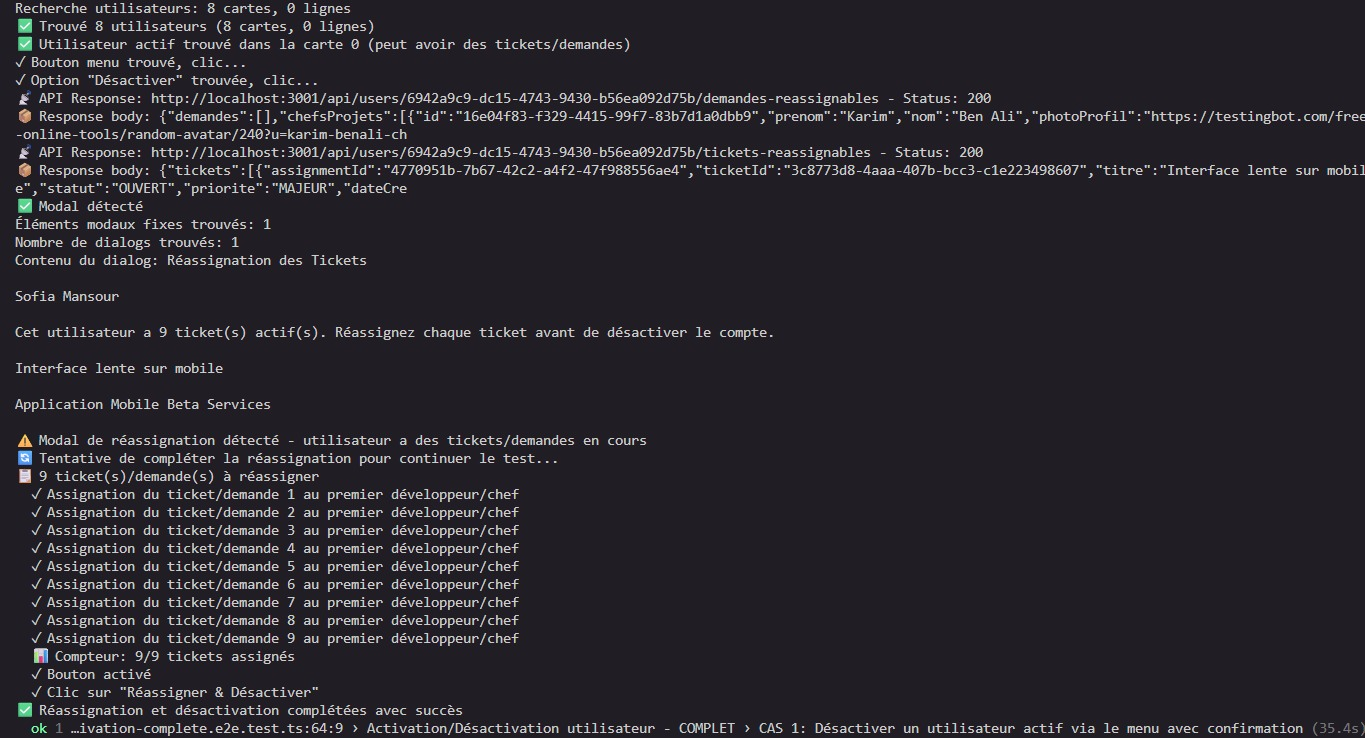
\includegraphics[width=0.68\textwidth,keepaspectratio]
  {Images/Test e2e desactiver utilisateu.png}
\caption{Tests End-to-End — Désactivation utilisateur via Playwright}
\label{fig:test_e2e_desactiver}
\end{figure}

\end{itemize}

% ---- Chapitre 4 ----
\hiddenpart{Sprint 2 -- Gestion Contractuelle et Traçabilité}
\chaptercover{4}{Sprint 2 -- Gestion Contractuelle et Traçabilité}

\section*{Introduction}

Le chapitre précédent était consacré à la mise en place des éléments de base de notre système. Nous y avons développé l'authentification et la gestion des utilisateurs avec leurs rôles et permissions. Nous avons aussi travaillé sur la gestion des clients et le processus de traitement des demandes d'inscription. L'ensemble de ces fonctionnalités a été testé et validé.
\newline Dans ce chapitre, nous passons au développement du cœur métier. Il s'agit principalement des contrats de maintenance avec leurs SLA, des projets et de leurs équipes, ainsi que de l'historique qui assure la traçabilité de toutes les modifications.
% ─────────────────────────────────────────────────────────────────────────────
% SECTION 1 : BACKLOG DU SPRINT 2
% ─────────────────────────────────────────────────────────────────────────────
\section{Sprint Planning Meeting }
La réunion de planification du deuxième sprint nous a permis de définir les objectifs à atteindre durant les trois prochaines semaines. Nous avons sélectionné les user stories prioritaires et estimé l'effort nécessaire pour chacune d'elles. Cette étape est importante pour que toute l'équipe comprenne bien le travail à réaliser.
\newline
\subsection{Objectif du Sprint}
Ce sprint vise à développer les fonctionnalités essentielles du système. L'objectif principal est de mettre en place la gestion des contrats de maintenance et d'assurer le suivi des engagements de service à travers leurs SLA, de faciliter la collaboration via l'affectation des équipes aux projets, et de garantir la traçabilité complète des opérations effectuées.
\subsubsection{Backlog du deuxième sprint}
\label{sec:backlog_sprint2}

Le tableau ci-dessous présente le Sprint Backlog détaillé avec les descriptions techniques et l'effort estimé pour chaque user story.
\newline
\textbf{1 : Effort faible, 2 : Effort moyen, 3 : Effort élevé}

\rowcolors{0}{}{}
\arrayrulecolor{black}
\renewcommand{\arraystretch}{1.3}
\small

\begin{longtable}{|C{1cm}|m{6.5cm}|m{7cm}|C{1cm}|}
\hline
\textbf{ID US} & \textbf{User Story} & \textbf{Description technique} & \textbf{Effort} \\
\hline
\endfirsthead

    \hline

\endhead

\hline
\endfoot

\hline
\endlastfoot
\multicolumn{4}{|l|}{\cellcolor{blue!20}\textbf{Epic 5 - Gestion des Clients}} \\
\hline
 US17 & En tant qu'\textbf{administrateur}, je souhaite créer un profil client afin de centraliser ses informations. &
\vspace{2mm}
\begin{itemize}[nosep, left=0pt, label={$\bullet$}]
\item Développer l’endpoint POST /clients pour orchestrer la création simultanée du compte CLIENT et du profil entreprise associé.  
\item  Implémenter un service de récupération automatique de logo (LogoService) établi sur le nom de la société
\item Intégrer une logique de gestion des projets historiques pour associer des projets passés, des chefs de projets et des membres d'équipe au nouveau client
\item Réaliser l'interface de formulaire
\end{itemize} & 1 \\
\hline

US18 & En tant qu’administrateur, je souhaite consulter la liste des clients  afin de visualiser les clients existants. &
\vspace{2mm}
\begin{itemize}[nosep, left=0pt, label={$\bullet$}]
\item Développer l’endpoint GET /clients intégrant une logique de filtrage RBAC.
\item Réaliser une interface de visualisation
\end{itemize} & 2 \\
\hline
US19 & En tant qu'\textbf{administrateur}, je souhaite consulter le profil détaillé d'un client afin de visualiser toutes ses informations. &
\begin{itemize}[nosep, left=0pt, label={$\bullet$}]
\item Développer l’endpoint GET /clients/:id pour récupérer les informations du client.
\item Réaliser une interface de profil structurée.
\item Développer des composants spécifiques pour l'affichage des informations secondaires       
\end{itemize} & 1 \\
\hline
US20 & En tant qu'\textbf{administrateur}, je souhaite modifier les informations d'un client afin de maintenir des données à jour. &
\begin{itemize}[nosep, left=0pt, label={$\bullet$}]
\item Développer l’endpoint PATCH /clients/:id permettant la mise à jour des informations des clients. 
\item Développer des contrôles d'intégrité côté serveur pour valider les formats de données.
\item Réaliser une interface d'édition fluide.
\end{itemize} & 2 \\
\hline
US21 & En tant qu'\textbf{administrateur}, je souhaite activer et désactiver un compte client afin de contrôler l'accès. &
\begin{itemize}[nosep, left=0pt, label={$\bullet$}]
\item Développer les endpoints de changement de statut (POST /desactiver, POST /reactiver)
\item Implémenter la vérification pour bloquer l'opération si le client possède des contrats actifs, des demandes en attente ou des tickets non résolus.  
\item Intégrer le EmailService pour l'envoi automatique de notifications transactionnelles de changement de statut.                           
\end{itemize} & 3 \\
\hline

US22 & En tant qu'\textbf{administrateur}, je souhaite imprimer l'annuaire d'un client afin de disposer d'une version papier. &
\begin{itemize}[nosep, left=0pt, label={$\bullet$}]
\item Développer l'endpoint POST /clients pour créer un client avec validation des données
\end{itemize} & 1 \\
\hline

US23 & En tant qu'\textbf{administrateur}, je souhaite créer un projet rattaché à un client afin d'organiser les interventions. &
\vspace{2mm}
\begin{itemize}[nosep, left=0pt, label={$\bullet$}]
\item Développer l'API de création avec validation des données
\item Gérer les relations projet-client et envoyer les notifications aux membres de l'équipe
\item Créer le formulaire multi-étapes avec sélection guidée 
\end{itemize} & 3 \\
\hline 
US24 & En tant qu'\textbf{administrateur}, je souhaite consulter la liste des projets afin de piloter l'activité. &
\vspace{2mm}
\begin{itemize}[nosep, left=0pt, label={$\bullet$}]
\item Développer l'API de consultation avec filtres et contrôler l'accès selon le rôle
\item Récupérer les données enrichies et paginer les résultats
\item Créer l'interface avec tableau, filtres avancés et proposer les vues multiples (liste/cartes/Kanban)
\end{itemize} & 2 \\
\hline
US25 & En tant qu'\textbf{administrateur}, je souhaite affecter des développeurs à un projet afin de constituer l'équipe. &
\vspace{2mm}
\begin{itemize}[nosep, left=0pt, label={$\bullet$}]
\item Développer l'API d'affectation avec workflow de validation
\item Calculer automatiquement la disponibilité et envoyer les notifications en temps réel à chaque étape
\item Créer les interfaces de gestion d'équipe avec suivi des propositions
\end{itemize} & 3 \\
\hline
US26 & En tant que \textbf{membre d'équipe}, je souhaite consulter les informations du projet afin de comprendre le contexte. &
\vspace{2mm}
\begin{itemize}[nosep, left=0pt, label={$\bullet$}]
\item Développer l'API de détail avec contrôle d'accès 
\item Créer la page détaillée organisée en sections avec les informations du projet
\end{itemize} & 1 \\
\hline


% Epic 2: Gestion des utilisateurs
\multicolumn{4}{|l|}{\cellcolor{blue!20}\textbf{Epic 7 -Gestion des Contrats}} \\
\hline

US28 & En tant qu’administrateur, je souhaite créer un contrat de maintenance afin de formaliser les engagements de service avec le client. & 
\vspace{2mm}
\begin{itemize}[nosep, left=0pt, label={$\bullet$}]
\item Développer l'API de création avec deux modes : formulaire manuel et upload PDF avec extraction automatique (pdf-parse + regex)
\item Implémenter l'extraction des données du PDF (référence, dates, montants, SLA, client, projet) et résolution automatique en base
\item Créer l'interface avec choix du mode, pré-remplissage automatique du formulaire et stockage avec hashage anti-doublon
\end{itemize}
& 2 \\
\hline

US29 & En tant qu’administrateur, je souhaite consulter la liste des contrats afin de suivre les engagements contractuels. & 
\vspace{2mm}
\begin{itemize}[nosep, left=0pt, label={$\bullet$}]
\item Développer l'API de consultation avec filtres avancés et contrôle d'accès RBAC
\item Récupérer les données enrichies avec pagination
\item Créer l'interface avec tableau, filtres, badges de statut et actions rapides (voir, modifier, archiver)
\end{itemize}
& 3 \\
\hline

US30 & En tant qu’administrateur, je souhaite recevoir des alertes avant l’expiration des contrats afin d’anticiper les renouvellements & 
\vspace{2mm} 
\begin{itemize}[nosep, left=0pt, label={$\bullet$}]
\item Développer le système d'alertes automatiques (30, 15, 7 jours avant expiration) avec CRON job
\item Envoyer les notifications par email et in-app avec détails du contrat
\item Créer l'interface d'alertes avec liste des contrats à renouveler
\end{itemize}
& 2 \\
\hline

US31 & En tant qu’administrateur, je souhaite archiver un contrat afin de conserver l’historique. & 
\vspace{2mm}
\begin{itemize}[nosep, left=0pt, label={$\bullet$}]
\item Développer l'API d'archivage avec vérifications (pas de demandes en cours, confirmation requise)
\item Gérer le changement de statut et conserver les données historiques avec motif d'archivage
\item Créer le dialogue de confirmation 
\end{itemize}
 & 3 \\
\hline

US32 & En tant que client, je souhaite demander la résiliation de mon contrat afin d’interrompre le service.& 
\vspace{2mm}
\begin{itemize}[nosep, left=0pt, label={$\bullet$}]
\item Développer l'API de demande de résiliation avec workflow (demande → validation admin → résiliation)
\item Envoyer les notifications aux administrateurs et gérer le statut du contrat
\item Créer le formulaire de demande avec motif obligatoire
\end{itemize}
 & 1 \\
\hline

US33 & En tant qu’administrateur, je souhaite résilier un contrat afin de l’interrompre avant terme. & 
\vspace{2mm} 
\begin{itemize}[nosep, left=0pt, label={$\bullet$}]
\item Développer l'API de résiliation avec validation
\item Gérer le changement de statut et notifier le client par email
\item Créer le dialogue de résiliation avec confirmation 
\end{itemize}
& 2 \\
\hline

\hline



US35 & En tant que chef de projet, je souhaite consulter les contrats dans un calendrier afin de visualiser les dates d’expiration& 
\vspace{2mm} 
\begin{itemize}[nosep, left=0pt, label={$\bullet$}]
\item Développer l'API de récupération des contrats avec dates (début, expiration) filtrées par période
\item Calculer les indicateurs (contrats expirant bientôt, contrats actifs) pour la vue calendrier
\item Créer la vue calendrier avec affichage des contrats par mois et code couleur selon le statut

\end{itemize}
& 1 \\
\hline
 US36 & En tant que \textbf{client}, je souhaite soumettre un retour d'expérience à l'expiration de mon contrat afin d'exprimer ma satisfaction.&
 \vspace{2mm} 
\begin{itemize}[nosep, left=0pt, label={$\bullet$}]
\item Développer l'endpoint POST /contrats/:id/feedback pour enregistrer la note, le commentaire et l'intention de renouvellement dans FeedbackExpirationContrat
\item Implémenter une logique de déclenchement automatique de notification aux administrateurs si le client souhaite renouveler
\item Réaliser le formulaire de feedback côté client avec affichage conditionnel selon le statut du contrat 

\end{itemize}
& 1 \\
\hline
US37 & En tant qu'\textbf{administrateur}, je souhaite générer un PDF formaté du contrat afin de le partager avec le client.&
 \vspace{2mm}
 &2 \\
 \hline
% Epic 3: Gestion des rôles et permissions
\multicolumn{4}{|l|}{\cellcolor{blue!20}\textbf{Epic 14 - Consulter journal d'activité}} \\
\hline

US95 & En tant qu’administrateur, je souhaite consulter l’historique complet de toutes les actions afin d’assurer la traçabilité. & 
\vspace{2mm}
\begin{itemize}[nosep, left=0pt, label={$\bullet$}]
\item Développer l'API de consultation avec pagination, filtres avancés et recherche textuelle
\item Récupérer les logs enrichis avec informations utilisateur et statistiques (taux de succès, actions fréquentes)
\item Créer l'interface avec tableau filtrable, timeline, graphiques de statistiques et vue détaillée par entité
\end{itemize}
 & 3 \\
\hline

US96 & En tant qu’administrateur, je souhaite exporter les logs d’audit afin de répondre aux exigences de conformité. & 
\vspace{2mm} 
\begin{itemize}[nosep, left=0pt, label={$\bullet$}]
\item Développer l'API d'export avec formats CSV et JSON, filtres personnalisables et limite de 10 000 enregistrements
\item Implémenter le nettoyage automatique des logs anciens
\item Créer l'interface d'export avec sélection de format, prévisualisation et téléchargement direct
\end{itemize}
& 2 \\
\hline

\end{longtable}


% ─────────────────────────────────────────────────────────────────────────────
% SECTION 2 : ANALYSE
% ─────────────────────────────────────────────────────────────────────────────

\section{Analyse}

\label{sec:analyse_sprint2}

\subsection{Diagramme des cas d'utilisation du deuxième sprint}

La figure ci-dessous présente le diagramme de cas d’utilisation du deuxième sprint : 

\begin{figure}[H]
        \centering
        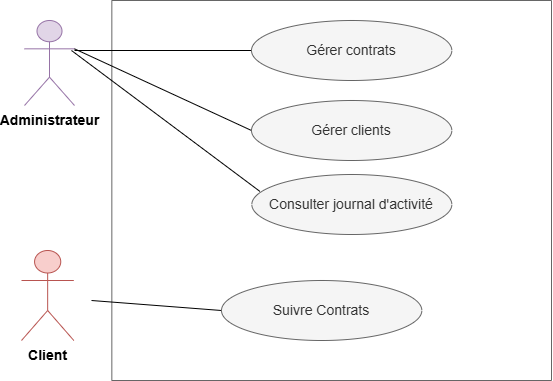
\includegraphics[width=0.85\textwidth,height=0.75\textheight,keepaspectratio]{Images/diagramme cas utilisation sprint2.png}
        \caption{Diagramme des cas d'utilisation du deuxième sprint}
        \label{fig:use_case_sprint2}
\end{figure}
Nous allons accompagner les cas d'utilisation d'un texte descriptif pour expliquer le scénario de chaque cas ainsi que ses exceptions.



\subsection{Analyse de la fonctionnalité « Gérer Contrats »}

Dans cette partie, nous allons présenter les cas d’utilisation relatifs à la gestion des Contrats afin de comprendre
les principales fonctionnalités du système, ce qui permet d’avoir une vue globale des interactions.
\subsubsection{Raffinement de cas d'utilisation « Gérer Contrats »}
Au cours de cette partie, nous allons analyser chaque cas d’utilisation raffiné pour le cas de gestion des Contrats :

\begin{figure}[H]
        \centering
        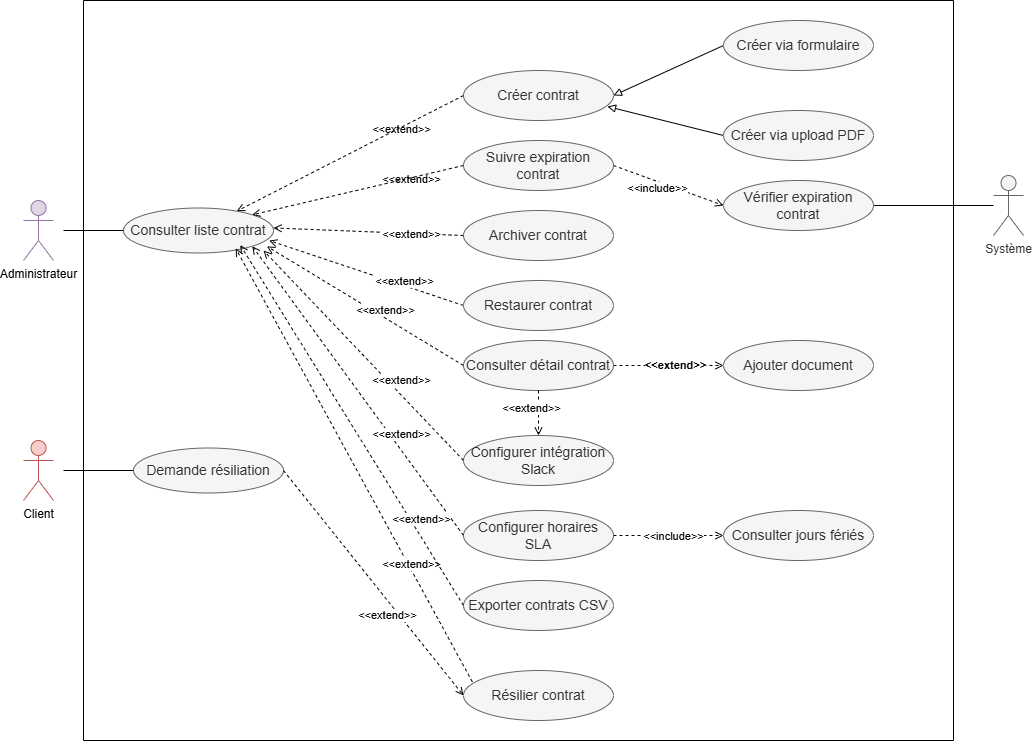
\includegraphics[width=0.9\textwidth,height=0.75\textheight,keepaspectratio]{Images/Diagramme de cas utilisation gestion contrat.png}
        \caption{Diagramme des cas d'utilisation « Gérer Contrats »}
        \label{fig:gerer_contrats}
\end{figure}

\subsubsection{Description textuelle de cas d'utilisation « Créer contrat »}
\vspace{-0.3cm}
\begin{table}[h]
\centering
\footnotesize
\renewcommand{\arraystretch}{1}

\begin{tabular}{|p{4.5cm}|p{12cm}|}
\hline
\textbf{Nom du cas d'utilisation} & Créer un contrat \\
\hline
\textbf{Acteurs} & Administrateur \\
\hline
\textbf{Préconditions} & 
L'utilisateur est authentifié.\newline
L'utilisateur possède la permission de créer des contrats. \newline
La liste des contrats est accessible.\\
\hline
\textbf{Postconditions} & 
  Le contrat est enregistré avec le statut ACTIF et une référence générée automatiquement.\newline
  Le contrat est visible dans la liste des contrats et lié au client sélectionné.\\
\hline
\textbf{Scénario principal} & 
\begin{minipage}[t]{\linewidth}
\begin{enumerate}[label=\arabic*., leftmargin=*]
 \item L'administrateur clique sur « Nouveau » depuis la liste des contrats.
    \item Le système propose deux modes : \textit{Saisie manuelle} ou \textit{Import PDF}.
    \item L'administrateur sélectionne \textit{Saisie manuelle} et confirme.
    \item L'administrateur renseigne les informations du contrat : client, projet, dates, montant, devise et taux de TVA.
    \item L'administrateur configure le niveau de service (SLA) avec les délais par priorité.
    \item L'administrateur valide le formulaire.
    \item Le système enregistre le contrat et redirige vers la liste des contrats.
  
\end{enumerate}
\vspace{2pt}
\end{minipage} \\
\hline
\textbf{Scénarios alternatifs} & 
\begin{itemize}[nosep,leftmargin=0.8cm,topsep=0pt,itemsep=2pt, label=$\bullet$]
    \item  L'administrateur choisit le mode 
    \textit{Import de document} et dépose un fichier PDF. Le système 
    extrait automatiquement les données et pré-remplit le formulaire. 
    L'administrateur vérifie les données, sélectionne le client et le 
    projet, puis valide.

\end{itemize} \\
\hline
\textbf{Scénarios d'exception} & 
\begin{itemize}[nosep,leftmargin=0.8cm,topsep=0pt,itemsep=2pt, label=$\bullet$]
         \item  Le système détecte qu'un contrat actif existe déjà pour ce client/projet et affiche un message de blocage.
    \item  Le système détecte que le client, les dates ou le montant ne sont pas renseignés et affiche un message d'erreur.
    \item Le système détecte que la date de début est antérieure à aujourd'hui ou que la date d'expiration est antérieure ou égale à la date de début et affiche un message d'erreur.
    \item Le système détecte que le montant saisi est nul ou non numérique et affiche un message d'erreur.
  
\end{itemize} \\
\hline
\end{tabular}
\caption{Description textuelle « Créer contrat »}
\end{table}
\vspace{-0.3cm}


\subsubsection{Description textuelle de cas d'utilisation « Archiver contrat »}
\vspace{-0.3cm}
\begin{table}[H]
\centering
\footnotesize
\renewcommand{\arraystretch}{1}

\begin{tabular}{|p{4.5cm}|p{12cm}|}
\hline
\textbf{Nom du cas d'utilisation} & Archiver un contrat \\
\hline
\textbf{Acteurs} & Administrateur \\
\hline
\textbf{Préconditions} &
  L'utilisateur est authentifié.\newline
  L'utilisateur possède la permission d'archiver des contrats.\newline
  Le contrat est expiré et non encore archivé.\\
\hline
\textbf{Postconditions} &
  Le contrat est marqué comme archivé et n'apparaît plus dans la 
  liste principale.\newline
  Le motif d'archivage est enregistré et associé au contrat.\\
\hline
\textbf{Scénario principal} &
  \begin{minipage}[t]{\linewidth}
  \begin{enumerate}[label=\arabic*., leftmargin=*]
    \item L'administrateur sélectionne un contrat expiré depuis la liste.
    \item L'administrateur clique sur « Archivage définitif » dans le 
    menu contextuel.
    \item Le système affiche un dialogue de confirmation demandant un 
    motif d'archivage.
    \item L'administrateur saisit un motif et confirme.
    \item Le système archive le contrat et met à jour la liste.
  \end{enumerate}
  \vspace{2pt}
  \end{minipage} \\
\hline
\textbf{Scénarios alternatifs} &
  \begin{itemize}[nosep,leftmargin=0.8cm,topsep=0pt,itemsep=2pt, label=$\bullet$]
    \item  L'administrateur sélectionne 
    plusieurs contrats expirés et clique sur « Archiver la sélection ». 
    Le système archive tous les contrats éligibles et affiche le nombre 
    de contrats archivés avec succès.
  \end{itemize} \\
\hline
\textbf{Scénarios d'exception} &
  \begin{itemize}[nosep,leftmargin=0.8cm,topsep=0pt,itemsep=2pt, label=$\bullet$]
    \item Le système détecte que le contrat 
    n'est pas encore expiré et bloque l'action d'archivage.
    \item  Le système détecte que le motif 
    saisi contient moins de 10 caractères et désactive le bouton de 
    confirmation.
  \end{itemize} \\
\hline
\end{tabular}
\caption{Description textuelle « Archiver contrat »}
\end{table}
\vspace{-0.3cm}

\subsubsection{Description textuelle de cas d'utilisation « Configurer intégration Slack »}
\vspace{-0.3cm}
\begin{table}[H]
\centering
\footnotesize
\renewcommand{\arraystretch}{1}
\begin{tabular}{|p{4.5cm}|p{12cm}|}
\hline
\textbf{Nom du cas d'utilisation} & Configurer intégration Slack \\
\hline
\textbf{Acteurs} & Administrateur \\
\hline
\textbf{Préconditions} &
  L'administrateur est authentifié.\newline
  Un contrat est sélectionné.\\
\hline
\textbf{Postconditions} &
  La configuration Slack est enregistrée et liée au contrat.\newline
  Les notifications sont actives selon les préférences choisies.\\
\hline
\textbf{Scénario principal} &
  \begin{minipage}[t]{\linewidth}
  \begin{enumerate}[label=\arabic*., leftmargin=*]
    \item L'administrateur clique sur « Intégration Slack » depuis 
    le menu contextuel du contrat.
    \item Le système affiche le dialogue de configuration Slack.
    \item L'administrateur saisit l'URL du webhook et le canal Slack.
    \item L'administrateur configure les types de notifications 
    souhaités : ticket créé, mise à jour, résolu, critique seulement.
    \item L'administrateur clique sur « Configurer ».
    \item Le système enregistre la configuration et l'associe 
    au contrat.
  \end{enumerate}
  \vspace{2pt}
  \end{minipage} \\
\hline
\textbf{Scénarios alternatifs} &
  \begin{itemize}[nosep,leftmargin=0.8cm,topsep=0pt,itemsep=2pt, label=$\bullet$]
    \item
    Le système détecte qu'une configuration Slack existe déjà pour 
    ce contrat et pré-remplit le formulaire. L'administrateur modifie 
    les champs souhaités et clique sur « Mettre à jour ».
    \item  Après sauvegarde, 
    l'administrateur clique sur « Tester ». Le système envoie un 
    message de test sur le canal Slack configuré.
    \item L'administrateur 
    clique sur le bouton de suppression. Le système supprime la 
    configuration Slack du contrat.
  \end{itemize} \\
\hline
\textbf{Scénarios d'exception} &
  \begin{itemize}[nosep,leftmargin=0.8cm,topsep=0pt,itemsep=2pt, label=$\bullet$]
    \item  Le système détecte 
    que le webhook URL ou le canal ne sont pas renseignés et affiche 
    un message d'erreur.
    \item Le système détecte que le webhook 
    URL est invalide lors du test et affiche un message d'erreur.
  \end{itemize} \\
\hline
\end{tabular}
\caption{Description textuelle « Configurer intégration Slack »}
\end{table}
\vspace{-0.3cm}



\subsection{Analyse de la fonctionnalité « Gérer clients »}

\subsubsection{Raffinement de cas d'utilisation « Gérer clients »}
Au cours de cette partie, nous allons analyser chaque cas d'utilisation raffiné pour le cas de gestion des clients :

\begin{figure}[H]
\centering
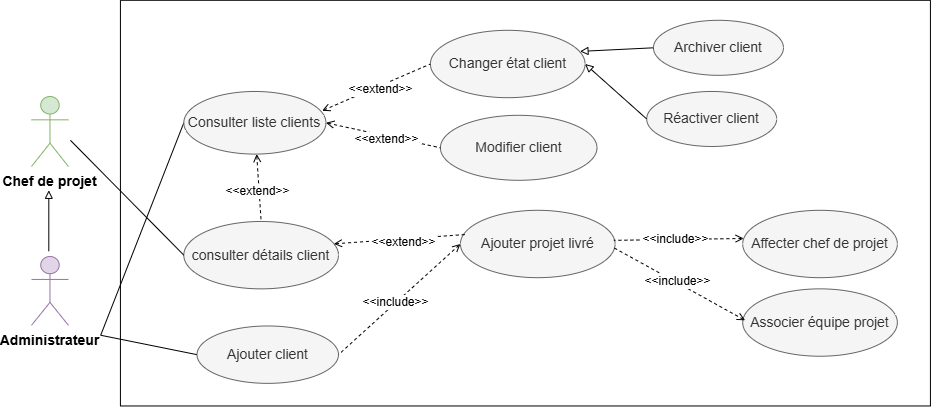
\includegraphics[width=0.8\textwidth,keepaspectratio]{Images/gerer client.drawio.png}
\caption{Raffinement de cas d'utilisation « Gérer clients »}
\label{fig:gerer_clients}
\end{figure}

\subsubsection{Description textuelle de cas d'utilisation « Consulter liste clients »}

\begin{table}[H]
\centering
\footnotesize
\renewcommand{\arraystretch}{1}
\caption{Description textuelle « Consulter liste clients »}
\begin{tabular}{|p{4.5cm}|p{12cm}|}
\hline
\textbf{Nom du cas d'utilisation} & Consulter liste clients \\
\hline
\textbf{Acteurs} & Administrateur, Chef de projet \\
\hline
\textbf{Préconditions} & L'utilisateur est authentifié\newline L'utilisateur possède la permission de consulter les clients\\
\hline
\textbf{Postconditions} & Liste des clients affichée\\
\hline
\textbf{Scénario principal} & 
\begin{minipage}[t]{\linewidth}
\begin{enumerate}[label=\arabic*., leftmargin=*]
\item L'utilisateur accède à la section "Clients".   
\item Le système affiche les clients sous forme de grille (par défaut).
\item L'utilisateur peut basculer entre trois modes d'affichage : grille, liste, ou vue par société.
\item L'utilisateur recherche un client en saisissant des informations clés dans la barre de recherche ou par des boutons de filtre (par statut, par secteur d'activité). 
\item Le système filtre les résultats.
\end{enumerate}
\vspace{2pt}
\end{minipage} \\
\hline
\textbf{Scénarios alternatifs} & \begin{itemize}[nosep,leftmargin=0.8cm,topsep=0pt,itemsep=2pt, label=$\bullet$]
\item L'utilisateur sélectionne la vue "Par société" pour regrouper les clients par société et visualiser les contacts associés à chaque société.
\item L'utilisateur clique sur le bouton « Exporter » pour télécharger la liste des clients (CSV, Excel).
\item L'utilisateur clique sur le bouton « Importer » pour ajouter plusieurs clients via un fichier (CSV, Excel).
\end{itemize} \\
\hline
\end{tabular}
\end{table}
\vspace{-0.3cm}

\subsubsection{Description textuelle de cas d'utilisation « Ajouter client »}

\begin{table}[H]
\centering
\footnotesize
\renewcommand{\arraystretch}{1}
\caption{Description textuelle « Ajouter client »}
\begin{tabular}{|p{4.5cm}|p{12cm}|}
\hline
\textbf{Nom du cas d'utilisation} & Ajouter un client \\
\hline
\textbf{Acteurs} & Administrateur \\
\hline
\textbf{Préconditions} & 
L'utilisateur est authentifié.\newline
L'utilisateur possède la permission de créer des clients. \newline
La liste des clients est accessible.\\
\hline
\textbf{Postconditions} & 
Le client est créé et enregistré dans le système. \newline
Le profil client associé est initialisé. \newline
Un message de confirmation est affiché. \\
\hline
\textbf{Scénario principal} & 
\begin{minipage}[t]{\linewidth}
\begin{enumerate}[label=\arabic*., leftmargin=*]
\item L'administrateur clique sur le bouton « Nouveau client ».
\item Le système affiche le formulaire de création.
\item L'administrateur saisit les informations du client : prénom, nom, e-mail et autres données requises.
\item L'administrateur renseigne ou sélectionne la société associée au client.
\item Si nécessaire, l'administrateur complète les informations de la société : nom, adresse, secteur d'activité et téléphone.
\item Le système peut récupérer automatiquement le logo de la société à partir d'une source externe, ainsi que l'adresse via un service de géocodage, si ces fonctionnalités sont activées.
\item L'administrateur valide le formulaire en cliquant sur « Créer le client ».
\item Le système vérifie la validité des données et l'unicité de l'e-mail.
\item Le système crée le client et associe son profil dans la base de données.
\item Le système envoie un e-mail de confirmation ou de bienvenue si cette fonctionnalité est prévue.
\item Le système affiche un message de succès et met à jour la liste des clients.
\end{enumerate}
\vspace{2pt}
\end{minipage} \\
\hline
\textbf{Scénarios alternatifs} & 
\begin{itemize}[nosep,leftmargin=0.8cm,topsep=0pt,itemsep=2pt, label=$\bullet$]
\item L'administrateur ajoute manuellement le logo de la société au lieu d'utiliser la récupération automatique.
\item L'administrateur associe le client à une société existante déjà enregistrée.
\item L'administrateur saisit manuellement l'adresse de la société lorsque la suggestion automatique du géocodage ne correspond pas.
\item L'administrateur complète plus tard certaines informations facultatives du client.
\end{itemize} \\
\hline
\textbf{Scénarios d'exception} & 
\begin{itemize}[nosep,leftmargin=0.8cm,topsep=0pt,itemsep=2pt, label=$\bullet$]
\item Un champ obligatoire est vide ou contient une valeur invalide.
\item L'adresse e-mail saisie est déjà utilisée par un autre utilisateur.
\item Le système rencontre une erreur lors de l'enregistrement du client.
\item L'administrateur tente de quitter le formulaire alors que des données ont déjà été saisies.
\end{itemize} \\
\hline
\end{tabular}
\end{table}
\vspace{-0.3cm}

% \subsubsection{Description textuelle de cas d'utilisation « Modifier client »}

% \begin{table}[H]
% \centering
% \footnotesize
% \renewcommand{\arraystretch}{1}
% \caption{Description textuelle « Modifier client »}
% \begin{tabular}{|p{4.5cm}|p{12cm}|}
% \hline
% \textbf{Nom du cas d'utilisation} & Modifier client \\
% \hline
% \textbf{Acteurs} & Administrateur \\
% \hline
% \textbf{Préconditions} & L'utilisateur est authentifié\newline L'utilisateur possède la permission de modifier les clients\newline Liste des clients affichée\\
% \hline
% \textbf{Postconditions} & Le client est modifié\\
% \hline
% \textbf{Scénario principal} & \begin{minipage}[t]{\linewidth}
% \begin{enumerate}[label=\arabic*., leftmargin=*]
% \item L'administrateur consulte la fiche du client choisi.                 
% \item L'administrateur clique sur le bouton (Modifier).                                                       
% \item Le système affiche le formulaire de modification.  
% \item L'administrateur modifie les informations souhaitées. 
% \item L'administrateur clique sur le bouton (Enregistrer).
% \item Le système met à jour les informations du client.
% \item Le système affiche le message de succès.
% \end{enumerate}
% \vspace{2pt}
% \end{minipage} \\
% \hline
% \textbf{Scénarios d'exception} & \begin{itemize}[nosep,leftmargin=0.8cm,topsep=0pt,itemsep=2pt, label=$\bullet$] 
% \item L'administrateur saisit un e-mail déjà utilisé par un autre utilisateur.
% \item L'administrateur tente de modifier un client ayant des contrats actifs sans validation.
% \end{itemize} \\
% \hline
% \end{tabular}
% \end{table}
% \vspace{-0.8cm}

\subsubsection{Description textuelle de cas d'utilisation « Consulter profil client »}

\begin{table}[H]
\centering
\footnotesize
\renewcommand{\arraystretch}{1}
\caption{Description textuelle « Consulter profil client »}
\begin{tabular}{|p{4.5cm}|p{12cm}|}
\hline
\textbf{Nom du cas d'utilisation} & Consulter profil client \\
\hline
\textbf{Acteurs} & Administrateur, Chef de projet, Client (son propre profil) \\
\hline
\textbf{Préconditions} & L'utilisateur est authentifié\newline L'utilisateur possède la permission de consulter les profils clients ou consulte son propre profil\newline Pour Chef de projet : le client doit être associé à au moins un de ses projets\\
\hline
\textbf{Postconditions} & Profil client consulté\\
\hline
\textbf{Scénario principal} & 
\begin{minipage}[t]{\linewidth}
\begin{enumerate}[label=\arabic*., leftmargin=*]
\item L'utilisateur accède au profil du client.
\item Le système affiche les informations personnelles et société.
\item Le système affiche les statistiques et éléments accessibles selon le rôle de l'utilisateur.
\item L'utilisateur peut naviguer vers les éléments disponibles (projets, demandes, tickets, documents).
\end{enumerate}
\vspace{2pt}
\end{minipage} \\
\hline
\textbf{Restrictions d'accès} & 
\begin{minipage}[t]{\linewidth}
\begin{itemize}[nosep,leftmargin=0.8cm,topsep=0pt,itemsep=2pt, label=$\bullet$]
\item Administrateur : accès complet (contrats, projets, demandes, tickets, notes privées, documents).
\item Chef de projet : accès limité aux projets où il est assigné et aux demandes/tickets liés à ces projets uniquement.
\item Client : accès à son propre profil, ses projets, demandes et tickets.
\end{itemize}
\vspace{2pt}
\end{minipage} \\
\hline
\textbf{Scénarios alternatifs} & \begin{itemize}[nosep,leftmargin=0.8cm,topsep=0pt,itemsep=2pt, label=$\bullet$]
\item L'utilisateur exporte les informations du profil en PDF.
\item L'utilisateur clique sur "Contacter" pour envoyer un e-mail ou un message via la messagerie interne de l'application.
\item L'utilisateur clique sur l'adresse de la société pour visualiser sa localisation sur une carte interactive.
\item L'administrateur ajoute une note privée sur le client.
\end{itemize} \\
\hline
\end{tabular}
\end{table}
\vspace{-0.3cm}

\subsubsection{Description textuelle de cas d'utilisation « Désactiver client »}

\begin{table}[H]
\centering
\footnotesize
\renewcommand{\arraystretch}{1}
\caption{Description textuelle « Désactiver un client »}
\begin{tabular}{|p{4.5cm}|p{12cm}|}
\hline
\textbf{Nom du cas d'utilisation} & Désactiver un client \\
\hline
\textbf{Acteurs} & Administrateur \\
\hline
\textbf{Préconditions} & L'utilisateur est authentifié\newline L'utilisateur possède la permission de désactiver les clients\newline Liste des clients affichée\newline Le client à désactiver doit être actuellement Actif\\
\hline
\textbf{Postconditions} & Le compte client est désactivé\\
\hline
\textbf{Scénario principal} & \begin{minipage}[t]{\linewidth}
\begin{enumerate}[label=\arabic*., leftmargin=*]
\item L'administrateur choisit un client dans la liste.                 
\item L'administrateur clique sur l'action (Désactiver).                                                     
\item Le système vérifie si le client possède des contrats actifs, des demandes en cours ou des tickets actifs.  
\item Le système affiche une boîte de dialogue de confirmation avec les détails des contrats, demandes et tickets actifs. 
\item L'administrateur confirme l'action.
\item Le système met à jour le statut du client.
\item Le système révoque les sessions actives (suppression des refresh tokens).
\item Le système envoie un e-mail automatique au contact principal du client pour l'informer de la désactivation.
\item Le système affiche le message de succès.
\end{enumerate}
\vspace{2pt}
\end{minipage} \\
\hline
\textbf{Scénarios d'exception} & \begin{itemize}[nosep,leftmargin=0.8cm,topsep=0pt,itemsep=2pt, label=$\bullet$] 
\item L'administrateur tente de désactiver un client qui possède des contrats actifs sans les clôturer.
\item L'administrateur tente de désactiver un client ayant des demandes en attente de traitement.
\item L'administrateur tente de désactiver un client ayant des tickets actifs non résolus.
\end{itemize} \\
\hline
\textbf{Scénarios alternatifs} & L'administrateur clôture les contrats, traite les demandes et résout les tickets avant la désactivation. \\
\hline
\end{tabular}
\end{table}
\vspace{-0.3cm}

\subsubsection{Description textuelle de cas d'utilisation « Réactiver client »}

\begin{table}[H]
\centering
\footnotesize
\renewcommand{\arraystretch}{1}
\caption{Description textuelle « Réactiver un client »}
\begin{tabular}{|p{4.5cm}|p{12cm}|}
\hline
\textbf{Nom du cas d'utilisation} & Réactiver un client \\
\hline
\textbf{Acteurs} & Administrateur \\
\hline
\textbf{Préconditions} & L'utilisateur est authentifié\newline L'utilisateur possède la permission de réactiver les clients\newline Le compte client doit être désactivé\\
\hline
\textbf{Postconditions} & Le compte client est réactivé\\
\hline
\textbf{Scénario principal} & \begin{minipage}[t]{\linewidth}
\begin{enumerate}[label=\arabic*., leftmargin=*]
\item L'administrateur consulte la liste des clients désactivés.
\item L'administrateur sélectionne un client à réactiver.
\item L'administrateur clique sur l'action (Réactiver le compte).
\item Le système affiche une confirmation.
\item L'administrateur confirme l'action.
\item Le système réactive le compte.
\item Le système envoie un e-mail au client.
\item Le système affiche le message de succès.
\end{enumerate}
\vspace{2pt}
\end{minipage} \\
\hline
\textbf{Scénarios d'exception} & Le client est déjà actif. \\
\hline
\end{tabular}
\end{table}
\vspace{-0.3cm}


\newpage

% ─────────────────────────────────────────────────────────────────────────────
% SECTION 3 : CONCEPTION
% ─────────────────────────────────────────────────────────────────────────────

\section{Diagramme de classes de deuxiéme sprint}

\section{Diagramme de séquence}
\subsection{Diagramme de séquences du cas d'utilisation « Demande Résiliation »}

\begin{figure}[H]
        \centering
        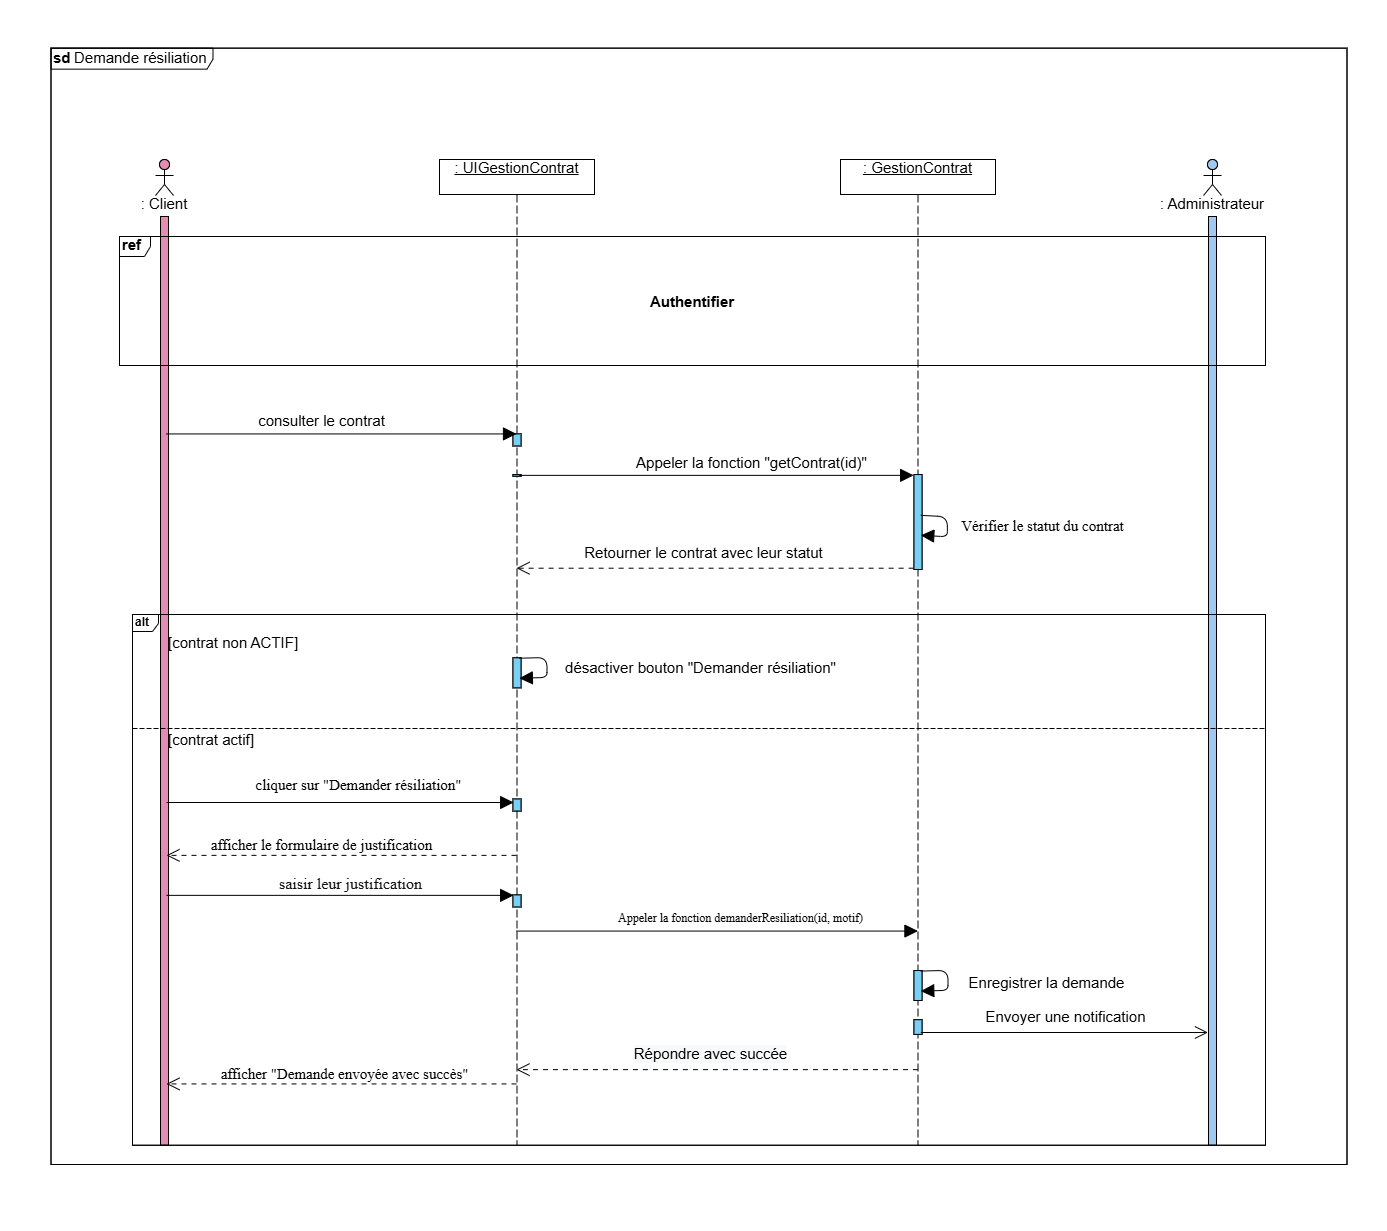
\includegraphics[width=0.7\textwidth,keepaspectratio]{Images/Diagramme de sequence Demande Resiliation.png}
        \caption{Diagramme de séquence du cas d'utilisation «  Demande Résiliation »}
        \label{fig:Diagramme de sequence Demande Resiliation}
\end{figure}
\subsection{Diagramme de séquences du cas d'utilisation « Résilier contrat »}

\begin{figure}[H]
        \centering
        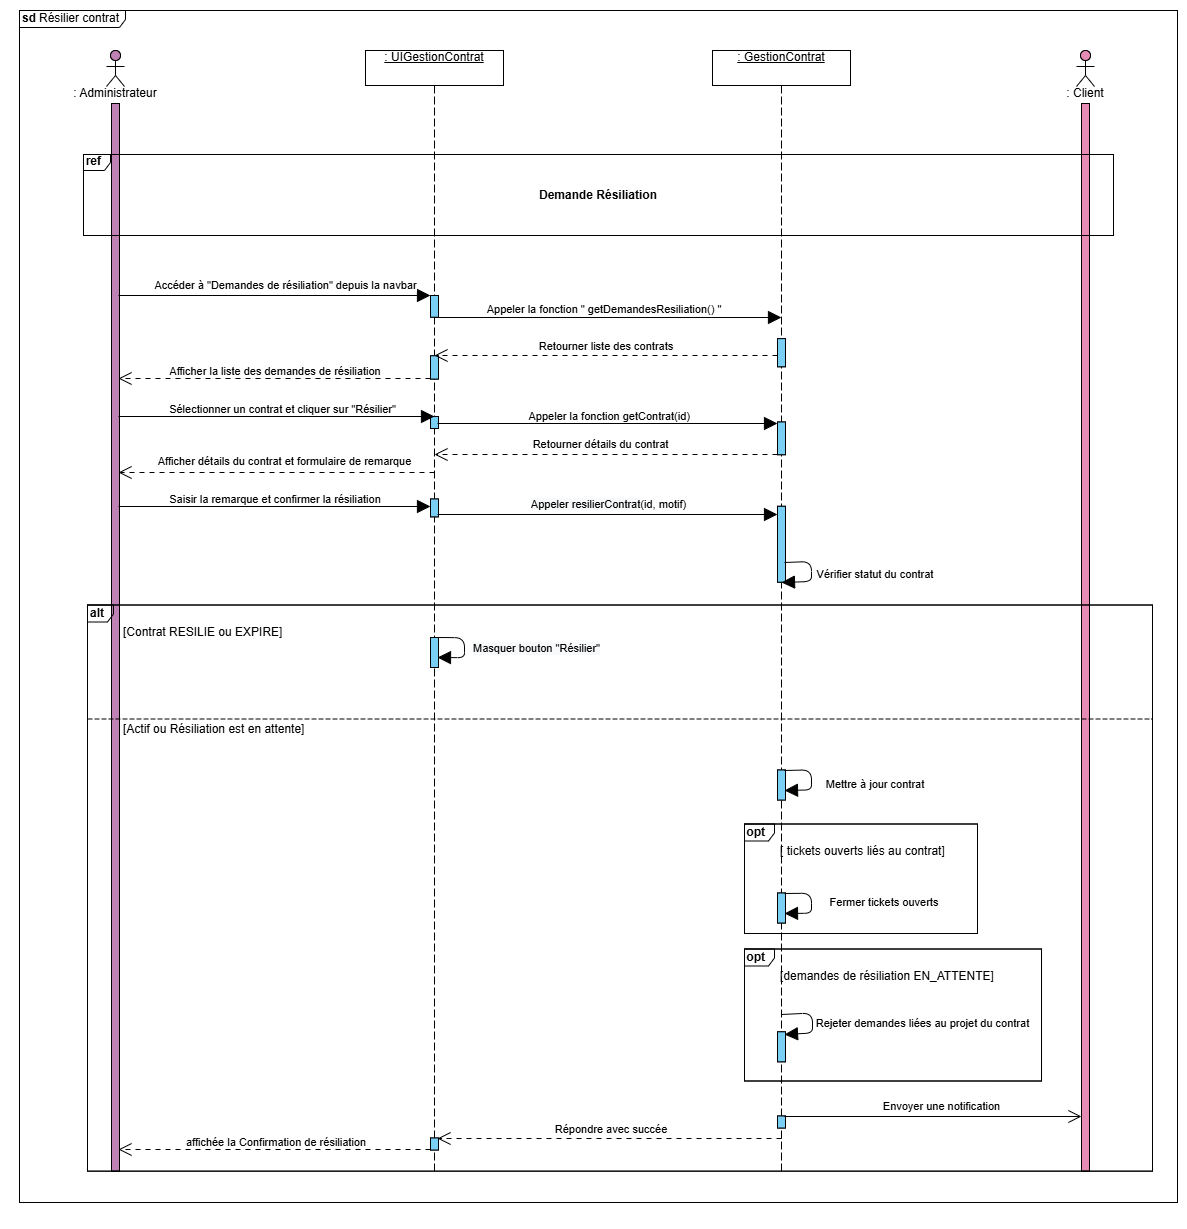
\includegraphics[width=0.7\textwidth,keepaspectratio]{Images/Diagramme de sequence de resilier contrat.png}
        \caption{Diagramme de séquence du cas d'utilisation « Résilier contrat »}
        \label{fig:Diagramme de sequence de resilier contrat}
\end{figure}

\newpage

% ─────────────────────────────────────────────────────────────────────────────
% SECTION 4 : RÉALISATION
% ─────────────────────────────────────────────────────────────────────────────

\section{Réalisation}
\label{sec:realisation_sprint2}

\subsection{Architecture technique}

Cette section présentera l'architecture technique mise en place pour le Sprint 2, incluant les modules de gestion des clients, projets et contrats.

\textit{[À compléter avec les détails d'implémentation]}

\subsection{Interfaces utilisateur}

Cette section présentera les principales interfaces développées durant le Sprint 2.

\textit{[À compléter avec les captures d'écran]}

\newpage

% ─────────────────────────────────────────────────────────────────────────────
% SECTION 5 : TESTS
% ─────────────────────────────────────────────────────────────────────────────

\section{Tests}
\label{sec:tests_sprint2}

\subsection{Tests unitaires}

Cette section présentera les tests unitaires réalisés pour valider les fonctionnalités du Sprint 2.

\textit{[À compléter avec les résultats des tests]}

\subsection{Tests d'intégration}

Cette section présentera les tests d'intégration effectués pour s'assurer du bon fonctionnement global du système.

\textit{[À compléter avec les résultats des tests]}


% ---- Chapitre 5 ----
\hiddenpart{Sprint 3 -- Gestion Opérationnelle et Assistance IA}
\chaptercover{5}{Sprint 3 -- GGestion Opérationnelle et Assistance IA}

\section*{Introduction}
\section*{Introduction}
Dans le chapitre précédent, nous avons mis en place la gestion des projets et des contrats, définissant ainsi le cadre contractuel et organisationnel de notre collaboration avec les clients. 
\newline Au cours de ce chapitre, nous présenterons les fonctionnalités constituant le cœur opérationnel de \textbf{SolidMaint} : la gestion des demandes clients et le cycle de vie des tickets de maintenance. Ce troisième sprint se concentre sur l'efficacité du traitement technique, le suivi précis du temps via le chronométrage et le respect rigoureux des engagements de service (SLA).

% ─────────────────────────────────────────────────────────────────────────────
% SECTION 1 : BACKLOG DU SPRINT 1
% ─────────────────────────────────────────────────────────────────────────────
\section{Sprint Planning Meeting }
La planification de ce troisième sprint est cruciale car elle porte sur les fonctionnalités les plus utilisées au quotidien par les clients et les développeurs. L'enjeu est de garantir une transition fluide entre le signalement d'un besoin et sa résolution technique.
L'objectif de ce sprint est de livrer le moteur de production de la plateforme. Cela inclut le module de soumission des demandes pour les clients, l'interface de qualification pour les chefs de projet, et l'environnement de travail des développeurs articulé autour d'un tableau Kanban et d'un système de chronométrage interactif.
\subsubsection{Backlog du premier sprint}
\label{sec:backlog_sprint1}

Voici l’ensemble des fonctionnalités issues du Product Backlog, qui seront réalisées dans le cadre de ce sprint opérationnel.
\newline
\textbf{1 : Effort faible, 2 : Effort moyen, 3 : Effort élevé}
\rowcolors{0}{}{}
\arrayrulecolor{black}
\renewcommand{\arraystretch}{1.3}
\small

\begin{longtable}{|C{1cm}|m{6.5cm}|m{7cm}|C{1cm}|}
\hline
\textbf{ID US} & \textbf{User Story} & \textbf{Description technique} & \textbf{Effort} \\
\hline
\endfirsthead

    \hline

\endhead

\hline
\endfoot

\hline
\endlastfoot

% Epic 1: Authentification et Sécurité
\multicolumn{4}{|l|}{\cellcolor{blue!20}\textbf{Epic 1 - Authentification et Sécurité}} \\
\hline

US01 & En tant qu'\textbf{utilisateur}, je souhaite m'authentifier avec email et mot de passe afin d'accéder à mes informations de manière sécurisée. & 
\vspace{2mm}
\begin{itemize}[nosep, left=0pt, label={$\bullet$}]
\item Développer l'endpoint \texttt{POST /api/auth/login}
\item Mettre en place la gestion de session via \textbf{JWT}
    (access token 15 min, refresh token 7 jours stocké en base)
\item Réaliser l'interface connexion login
\item Consommer l'API d'authentification
\item Gérer les tentatives échouées (3 essais) avec verrouillage temporaire
\end{itemize} & 2 \\
\hline

US02 & En tant qu'\textbf{utilisateur}, je souhaite réinitialiser mon mot de passe afin de retrouver l'accès à mon compte. & 
\vspace{2mm}
\begin{itemize}[nosep, left=0pt, label={$\bullet$}]
\item Développer les endpoints
    \texttt{POST /api/auth/mot-de-passe-oublie} et
    \texttt{POST /api/auth/reinitialiser-mot-de-passe}
  \item Créer les formulaires « mot de passe oublié » et
    de réinitialisation côté Next.js
  \item Générer un token sécurisé (bcrypt) avec expiration
    de \textbf{1 heure}, stocké dans
    \texttt{TokenReinitialisationMotDePasse}
  \item Invalider les anciens tokens non utilisés à chaque
    nouvelle demande
  \item Configurer l'envoi d'un e-mail de réinitialisation
    et d'un e-mail de confirmation via \textbf{Nodemailer}
\end{itemize} & 2 \\
\hline

US03 & En tant qu'\textbf{utilisateur}, je souhaite m'authentifier via Google ou GitHub afin de me connecter rapidement sans créer de compte. & 
\vspace{2mm}
\begin{itemize}[nosep, left=0pt, label={$\bullet$}]
\item Intégrer les stratégies OAuth2 via
    \texttt{passport-google-oauth20} et \texttt{passport-github2}
    dans NestJS (\texttt{@nestjs/passport})
\item Implémenter les routes \texttt{GET /api/auth/google},\texttt{GET /api/auth/github} et leurs callbacks
  \item Si l'utilisateur existe en base et est actif :
    générer les tokens JWT et rediriger vers le frontend
    avec \texttt{?oauth=success}
\item Vérifier l'existence de l'utilisateur en base de données et une demande d'inscription OAuth est envoyée à l'admin
\item Implémenter les routes /auth/google, /auth/github et leurs callbacks, avec génération d'un JWT
\item Implémenter les boutons OAuth sur la page de login
\end{itemize} & 3 \\
\hline

US04 & En tant qu'\textbf{utilisateur}, je souhaite me déconnecter de la plateforme afin de sécuriser ma session. & 
\vspace{2mm}
\begin{itemize}[nosep, left=0pt, label={$\bullet$}]
\item Développer l'endpoint POST /auth/logout avec révocation du refresh token en base
\item Supprimer \texttt{accessToken}, \texttt{refreshToken}
    et \texttt{user} du \texttt{localStorage}
\item Vider le cache React Query (\texttt{queryClient.clear()})
\item Réaliser le bouton de déconnexion 
\end{itemize} & 1 \\
\hline

US05 & En tant qu'\textbf{utilisateur}, je souhaite que mon compte soit protégé contre les tentatives de connexion malveillantes afin de garantir la sécurité de mes données. & 
\vspace{2mm}
\begin{itemize}[nosep, left=0pt, label={$\bullet$}]
  \item Implémenter le compteur de tentatives échouées
    (\texttt{tentativesConnexionEchouees}) en base de données
  \item Verrouiller le compte après \textbf{3 tentatives échouées}
    pendant \textbf{1 minute} via le champ
    \texttt{compteVerrouilleJusquA}
  \item Réinitialiser le compteur à 0 après une connexion réussie
  \item Appliquer le rate limiting global via
    \texttt{@nestjs/throttler} sur les endpoints publics
\end{itemize} & 2 \\
\hline

% Epic 2: Gestion des utilisateurs
\multicolumn{4}{|l|}{\cellcolor{blue!20}\textbf{Epic 2 - Gestion des utilisateurs}} \\
\hline

US06 & En tant qu'\textbf{utilisateur}, je souhaite gérer mon profil afin que mes informations soient toujours à jour. & 
\vspace{2mm}
\begin{itemize}[nosep, left=0pt, label={$\bullet$}]
\item Développer les endpoints \texttt{GET /api/profil} et \texttt{PUT /api/profil}
\item Implémenter l'upload de la photo de profil \texttt{POST /api/profil/upload-photo}
\item Développer le changement de mot de passe via
    \texttt{POST /api/profil/change-password}
    avec vérification de l'ancien mot de passe (bcrypt)
\item Gérer les e-mails secondaires :
    \texttt{GET/POST/DELETE /api/profil/emails} et
    \texttt{PATCH /api/profil/emails/principal}
\item Réaliser l'interface profil côté Next.js  avec formulaire prérempli
\end{itemize} & 2 \\
\hline

US07 & En tant qu'\textbf{administrateur}, je souhaite créer des utilisateurs afin de gérer les accès au système. & 
\vspace{2mm}
\begin{itemize}[nosep, left=0pt, label={$\bullet$}]
\item Développer l'endpoint \texttt{POST /api/users}
\item Générer automatiquement un mot de passe temporaire haché via \textbf{bcrypt} (facteur 10)
\item Générer un token de réinitialisation (1 heure) et construire le lien de réinitialisation
\item Créer automatiquement le \texttt{ProfilEmploye}
    avec matricule \texttt{EMP-\{id\}} si le rôle n'est pas CLIENT
\item Valider les données d'entrée via \textbf{class-validator}
  \item Envoyer un e-mail de bienvenue via \textbf{Nodemailer}
    contenant le mot de passe temporaire et le lien de
    réinitialisation
  \item Réaliser le formulaire d'ajout côté Next.js
\end{itemize} & 3 \\
\hline

US08 & En tant qu'\textbf{administrateur}, je souhaite modifier les informations d'un utilisateur afin de maintenir des données à jour. & 
\vspace{2mm}
\begin{itemize}[nosep, left=0pt, label={$\bullet$}]
\item Développer l'endpoint \texttt{PUT /api/users/:id}
\item Sécuriser l'accès à l'endpoint pour les administrateurs uniquement
\item Valider les données via \textbf{class-validator}
\item Réaliser le formulaire de modification côté Next.js
\end{itemize} & 2 \\
\hline

US09 & En tant qu'\textbf{administrateur}, je souhaite activer et désactiver un compte utilisateur afin de contrôler l'accès au système. & 
\vspace{2mm}
\begin{itemize}[nosep, left=0pt, label={$\bullet$}]
\item Développer les endpoints \texttt{PATCH /api/users/:id/desactiver} et \texttt{PATCH /api/users/:id/reactiver}
\item Implémenter les vérifications de réassignation des tickets et des demandes en cas de désactivation
\item Envoyer des notifications pour informer l'utilisateur de l'activation ou désactivation de son compte
\item Réaliser les boutons d'action avec appels des API
\end{itemize} & 3 \\
\hline

US10 & En tant qu'\textbf{administrateur}, je souhaite consulter la liste des utilisateurs afin de visualiser et gérer efficacement les comptes. & 
\vspace{2mm}
\begin{itemize}[nosep, left=0pt, label={$\bullet$}]
\item Développer l'endpoint \texttt{GET /api/users}
\item Réaliser l'interface d'administration avec vue grille
    et vue liste, filtres par statut et par rôle,
    barre de recherche dynamique

\end{itemize} & 1 \\
\hline

US11 & En tant qu'\textbf{utilisateur}, je souhaite consulter l'historique de mes activités afin de suivre mes actions dans le système. & 
\vspace{2mm}
\begin{itemize}[nosep, left=0pt, label={$\bullet$}]
\item Développer l'endpoint \texttt{GET /api/users/:id/activities} pour récupérer l'historique
\item Implémenter la logique de filtrage dans le backend en utilisant l'opérateur contains
\item Implémenter une barre de recherche dynamique
\item Réaliser l'interface timeline avec filtres par date et type d'action
\end{itemize} & 2 \\
\hline

% Epic 3: Gestion des rôles et permissions
\multicolumn{4}{|l|}{\cellcolor{blue!20}\textbf{Epic 3 - Gestion des rôles et permissions}} \\
\hline

US12 & En tant qu'\textbf{administrateur}, je souhaite gérer des rôles afin de structurer les accès au système. & 
\vspace{2mm}
\begin{itemize}[nosep, left=0pt, label={$\bullet$}]
\item Développer les endpoints CRUD pour la gestion complète des rôles
\item Implémenter le PermissionsGuard et le décorateur @Permissions pour sécuriser les routes du backend 
\item Réaliser l'interface de gestion sous forme de matrice
\end{itemize} & 3 \\
\hline

US13 & En tant qu'\textbf{administrateur}, je souhaite attribuer des permissions granulaires aux rôles afin de contrôler précisément les accès. & 
\vspace{2mm}
\begin{itemize}[nosep, left=0pt, label={$\bullet$}]
\item Développer l’endpoint PATCH /roles-permissions/roles/:id/sync pour synchroniser dynamiquement les associations entre un rôle et ses permissions. 
\item Implémenter la logique de mise à jour atomique                                                                                                                                                                                                                       
\item Développer l'interface interactive de type "Matrice de contrôle d'accès" 

\end{itemize} & 2 \\
\hline
US14 & En tant qu'\textbf{administrateur}, je souhaite consulter la matrice rôles-permissions afin de visualiser rapidement les droits de chaque rôle. & 
\vspace{2mm}
\begin{itemize}[nosep, left=0pt, label={$\bullet$}]
\item Développer l’endpoint GET /roles-permissions/matrix ) pour récupérer les données 
\item Implémenter la logique de structuration des données au format JSON                
\item Réaliser l’interface de visualisation de type "Heatmap" ou "Tableau de bord"

\end{itemize} & 3 \\
\hline

% Epic 4: Demandes d'inscription OAuth
\multicolumn{4}{|l|}{\cellcolor{blue!20}\textbf{Epic 4 - Demandes d'inscription OAuth}} \\
\hline

US15 & En tant qu'\textbf{utilisateur externe}, je souhaite demander l'accès via OAuth afin de m'inscrire facilement. & 
\vspace{2mm}
\begin{itemize}[nosep, left=0pt, label={$\bullet$}]
\item Développer l'endpoint POST /auth/oauth/request pour créer une demande
\item Enregistrer la demande en base avec statut EN\_ATTENTE
\item Implémenter l'envoi de notification à l'administrateur via email et in-app
\item Réaliser l'interface de demande d'accès
\end{itemize} & 3 \\
\hline

US16 & En tant qu'\textbf{administrateur}, je souhaite valider ou rejeter les demandes d'inscription OAuth afin de contrôler les accès. & 
\vspace{2mm}
\begin{itemize}[nosep, left=0pt, label={$\bullet$}]
\item Développer les endpoints PATCH /auth/oauth/requests/:id/approve et /reject
\item Implémenter la création automatique du compte utilisateur lors de l'approbation
\item Configurer l'envoi d'emails de confirmation ou rejet via Nodemailer
\item Réaliser l'interface de gestion des demandes avec actions d'approbation/rejet
\end{itemize} & 3 \\
\hline
% Epic 4: Demandes d'inscription OAuth


\end{longtable}



% ─────────────────────────────────────────────────────────────────────────────
% SECTION 2 : ANALYSE
% ─────────────────────────────────────────────────────────────────────────────

\section{Analyse}
Dans cette phase, nous traduisons les besoins opérationnels en spécifications techniques, en mettant l'accent sur les transitions de statuts et les règles de gestion du temps de travail.
\subsection{Diagramme des cas d'utilisation du troisième sprint}
La figure ci-dessous présente le diagramme de cas d’utilisation du troisième sprint, centré sur le flux de traitement des incidents :
\begin{figure}[H]
        \centering
        \includegraphics[width=0.85\textwidth,height=0.60\textheight,keepaspectratio]{Images/Diagramme_cas_utilisation_sprint3.png}
        \caption{Diagramme des cas d'utilisation du troisième sprint}
        \label{fig:use_case_sprint3}
\end{figure}
\subsection{Description textuelle du cas d'utilisation « Convertir demande en ticket »}
Ce cas d'utilisation est le point de pivot entre le client et l'équipe technique.
\begin{table}[H]
\centering
\footnotesize
\renewcommand{\arraystretch}{1}
\begin{tabular}{|p{4.5cm}|p{12cm}|}
\hline
\textbf{Nom du cas d'utilisation} & Convertir une demande en ticket \\
\hline
\textbf{Acteurs} & Chef de projet \\
\hline
\textbf{Préconditions} & Une demande client est au statut \textit{EN\_ATTENTE} \\
\hline
\textbf{Postconditions} & Un ticket est créé, lié à la demande initiale, et les SLA sont initialisés \\
\hline
\textbf{Scénario principal} &
\begin{minipage}[t]{\linewidth}
\begin{enumerate}[label=\arabic*., nosep,leftmargin=0.8cm,topsep=0pt,itemsep=2pt]
\item Le Chef de projet accède à la liste des demandes en attente.
\item Il sélectionne une demande pour examiner son contenu et les pièces jointes.
\item Il valide la demande en définissant la priorité (Mineur, Majeur, Critique) et le type de maintenance.
\item Le système crée automatiquement le ticket avec un numéro de suivi unique.
\item Le système calcule les dates d'échéance selon la configuration SLA du contrat associé.
\item Le système notifie le client du passage en traitement technique.
\end{enumerate}
\vspace{2pt}
\end{minipage} \\
\hline
\textbf{Scénarios d'exception} &
\begin{itemize}[nosep,leftmargin=0.8cm,topsep=0pt,itemsep=2pt, label=$\bullet$]
\item La demande est incomplète : le CP demande des informations complémentaires (statut \textit{INFOS\_REQUISES}).
\item La demande est hors périmètre : le CP rejette la demande avec un motif obligatoire.
\end{itemize} \\
\hline
\end{tabular}
\caption{Description textuelle du cas « Convertir demande en ticket »}
\end{table}
\subsection{Description textuelle du cas d'utilisation « Gérer le chronomètre »}
Ce cas d'utilisation permet un suivi granulaire de l'effort fourni sur chaque ticket.
\begin{table}[H]
\centering
\footnotesize
\renewcommand{\arraystretch}{1}
\begin{tabular}{|p{4.5cm}|p{12cm}|}
\hline
\textbf{Nom du cas d'utilisation} & Gérer le chronomètre de travail \\
\hline
\textbf{Acteurs} & Développeur \\
\hline
\textbf{Préconditions} & Le développeur est assigné au ticket et celui-ci est au statut \textit{OUVERT} ou \textit{EN\_COURS} \\
\hline
\textbf{Postconditions} & Une session de travail est enregistrée et le temps passé sur le ticket est cumulé \\
\hline
\textbf{Scénario principal} &
\begin{minipage}[t]{\linewidth}
\begin{enumerate}[label=\arabic*., nosep,leftmargin=0.8cm,topsep=0pt,itemsep=2pt]
\item Le développeur ouvre la vue détail du ticket assigné.
\item Il clique sur le bouton « Démarrer » pour lancer le suivi.
\item Le système enregistre l'heure précise de début et change le statut du ticket à \textit{EN\_COURS}.
\item Le développeur effectue ses tâches techniques.
\item Il clique sur « Arrêter » une fois l'intervention terminée ou pour faire une pause.
\item Le système calcule la durée de la session, l'ajoute au total du ticket et clôture la session de travail.
\end{enumerate}
\vspace{2pt}
\end{minipage} \\
\hline
\textbf{Scénarios d'exception} &
\begin{itemize}[nosep,leftmargin=0.8cm,topsep=0pt,itemsep=2pt, label=$\bullet$]
\item Le développeur oublie de couper le chrono : il peut modifier manuellement la durée avec une justification (traçabilité).
\end{itemize} \\
\hline
\end{tabular}
\caption{Description textuelle du cas « Gérer le chronomètre »}
\end{table}
% ─────────────────────────────────────────────────────────────────────────────
% SECTION 3 : CONCEPTION
% ─────────────────────────────────────────────────────────────────────────────
\section{Conception}
La conception du Sprint 3 s'appuie sur une modélisation rigoureuse des transitions de statuts et de la logique temporelle.
\subsection{Diagramme de classes du troisième sprint}
Le diagramme suivant détaille la structure des entités \texttt{Ticket}, \texttt{Demande}, et \texttt{SessionTravail}, ainsi que leurs relations avec les contrats (SLA).
\begin{figure}[H]
        \centering
        \includegraphics[width=1\textwidth,keepaspectratio]{Images/diag_classe_sprint3.png}
        \caption{Diagramme de classes du Sprint 3 - Cœur opérationnel}
        \label{fig:diag_classe_sprint3}
\end{figure}
\section{Diagramme de séquence}
\subsection{Diagramme de séquences du cas d'utilisation « Conversion Demande en Ticket »}
Ce diagramme illustre le processus de validation métier et la création automatisée des entités techniques.
\begin{figure}[H]
        \centering
        \includegraphics[width=0.75\textwidth,keepaspectratio]{Images/diag_seq_conversion.png}
        \caption{Diagramme de séquence du cas « Conversion Demande en Ticket »}
        \label{fig:seq_conversion}
\end{figure}
\subsection{Diagramme de séquences du cas d'utilisation « Signalement de blocage »}
Ce diagramme détaille comment un signalement de blocage par un développeur suspend automatiquement le décompte du délai SLA.
\begin{figure}[H]
        \centering
        \includegraphics[width=0.75\textwidth,keepaspectratio]{Images/diag_seq_blocage.png}
        \caption{Diagramme de séquence du cas « Signalement de blocage »}
        \label{fig:seq_blocage}
\end{figure}
\section{Schéma relationnel}
\textbf{Ticket} (\underline{idTicket}, \textbf{\#idDemande}, titre, description, statut, priorite, type, \textbf{\#idProjet}, dateEcheanceSLA, tempsEstime)
\newline
\textbf{SessionTravail} (\underline{idSession}, \textbf{\#idTicket}, \textbf{\#idUtilisateur}, dateDebut, dateFin, dureeSecondes, descriptionTravail)
\newline
\textbf{DemandeClient} (\underline{idDemande}, \textbf{\#idProfilC}, titre, description, statut, dateCreation, \textbf{\#idContrat})
\newline
\textbf{TicketBlocage} (\underline{idBlocage}, \textbf{\#idTicket}, raison, statutBlocage, dateSignalement, dateResolution)
% ─────────────────────────────────────────────────────────────────────────────
% SECTION 4 : RÉALISATION
% ─────────────────────────────────────────────────────────────────────────────
\section{Réalisation}
Après avoir analysé les besoins et conçu les solutions, nous passons maintenant à la réalisation. Dans cette phase, nous avons développé toutes les user stories planifiées dans le sprint backlog. Cette section présente le diagramme de composants qui montre l'architecture de notre application, ainsi que les interfaces utilisateur que nous avons créées pour répondre aux besoins des utilisateurs.
\label{sec:realisation_sprint1}

\subsection{Diagramme de composants}


\subsection{Description des interfaces}
Cette section présente les principales interfaces utilisateur développées lors du premier sprint.

\subsubsection{Interface de connexion}
\begin{figure}[H]
\centering
%\includegraphics[width=0.75\textwidth,keepaspectratio]{Images/interface_connexion.png}
\caption{Interface de connexion — authentification classique et OAuth}
\label{fig:interface_connexion}
\end{figure}
La page de connexion propose deux modes d'authentification : le formulaire
classique (e-mail + mot de passe) et les boutons OAuth (Google, GitHub).
En cas de compte inexistant, le visiteur est redirigé vers un flux de
demande d'inscription.

\subsubsection{Interface de réinitialisation du mot de passe}
\begin{figure}[H]
\centering
%\includegraphics[width=0.75\textwidth,keepaspectratio]{Images/interface_reset_password.png}
\caption{Interface de réinitialisation du mot de passe}
\label{fig:interface_reset}
\end{figure}
Cette interface permet à l'utilisateur de saisir son adresse e-mail pour
recevoir un lien de réinitialisation valable 1 heure.

\subsubsection{Interface de gestion des utilisateurs}
\begin{figure}[H]
\centering
%\includegraphics[width=0.85\textwidth,keepaspectratio]{Images/interface_users.png}
\caption{Interface d'administration — liste des utilisateurs}
\label{fig:interface_users}
\end{figure}
L'administrateur dispose d'une vue en grille ou en liste, avec filtres par
statut et par rôle, barre de recherche et actions rapides (modifier,
désactiver, voir le profil).

\subsubsection{Interface de gestion des rôles et permissions}
\begin{figure}[H]
\centering
%\includegraphics[width=0.85\textwidth,keepaspectratio]{Images/interface_roles_permissions.png}
\caption{Interface d'administration — gestion des rôles et permissions}
\label{fig:interface_roles}
\end{figure}
La matrice des permissions affiche les rôles en colonnes et les catégories
de permissions en lignes, avec des cases à cocher pour une attribution
visuelle et intuitive.

\subsubsection{Interface de gestion des demandes d'inscription OAuth}
\begin{figure}[H]
\centering
%\includegraphics[width=0.85\textwidth,keepaspectratio]{Images/interface_demandes_oauth.png}
\caption{Interface d'administration — demandes d'inscription OAuth}
\label{fig:interface_oauth}
\end{figure}
L'administrateur consulte les demandes en attente, visualise les
informations récupérées via OAuth et peut approuver ou refuser chaque
demande avec un motif de refus facultatif.

% ─────────────────────────────────────────────────────────────────────────────
% SECTION 5 : TESTS
% ─────────────────────────────────────────────────────────────────────────────
\section{Tests et Validation}
La phase de test est essentielle pour garantir la qualité et la fiabilité de la solution. Elle valide que chaque fonctionnalité répond aux exigences métier et identifie les anomalies avant la mise en production. Dans ce sprint, nous avons testé les mécanismes d'authentification, la gestion des utilisateurs et le contrôle d'accès (RBAC) pour assurer la robustesse de nos implémentations.

\subsection{Stratégie de tests adoptée}
Afin de garantir la qualité et la fiabilité de l'application, nous avons adopté une stratégie de tests structurée, reposant sur une répartition des vérifications à plusieurs niveaux. Cette approche permet d'assurer une bonne couverture fonctionnelle avec un temps d'exécution raisonnable, tout en facilitant l'identification rapide des anomalies.

Les tests ont été organisés par module fonctionnel afin d'assurer une meilleure traçabilité des vérifications effectuées. Ainsi, les tests unitaires couvrent les règles métier les plus fines, les tests d'intégration valident les échanges avec l'API, et les tests End-to-End reproduisent les scénarios complets d'utilisation de l'application.

La pyramide de tests se compose donc de trois niveaux complémentaires :


\subsubsection{Tests unitaires}
\label{sec:tests_unitaires}

Les tests unitaires ont été réalisés à l'aide du framework \textbf{Vitest},
en isolant chaque service du reste de l'application grâce à des mocks
Prisma. Cette approche garantit l'indépendance des tests et permet une
détection précoce des anomalies dès la phase de développement. Trois
modules prioritaires ont été couverts : l'authentification, le contrôle
d'accès basé sur les rôles (RBAC) et la gestion des clients.

\vspace{4pt}
\noindent\textbf{Bilan : 45 tests exécutés — 45 réussis — 0 échec.}
\vspace{6pt}

\begin{itemize}[leftmargin=0pt]

% ── 1. Authentification ───────────────────────────────────────────────────────
\item[$\square$] \textbf{Module Authentification}
\hfill\textit{Méthodes : \texttt{login()} ·
\texttt{demanderReinitialisationMotDePasse()} ·
\texttt{reinitialiserMotDePasse()}}

\noindent Cette suite valide le processus d'authentification classique,
la génération des jetons JWT et le mécanisme de réinitialisation du mot
de passe. Les cas suivants ont été couverts :

\begin{itemize}[label=$\bullet$, nosep, itemsep=2pt]
  \item Un utilisateur actif fournit des identifiants valides : les jetons
    \texttt{accessToken} et \texttt{refreshToken} sont générés
    correctement.
  \item L'adresse e-mail fournie n'existe pas en base de données : la
    connexion est rejetée avec le code \texttt{401 Unauthorized}.
  \item Le mot de passe fourni est incorrect : la connexion est rejetée
    avec le code \texttt{401 Unauthorized}.
  \item L'utilisateur échoue l'authentification \textbf{3 fois
    consécutives} : le compte est verrouillé automatiquement pendant
    \textbf{1 minute} (\texttt{maxLoginAttempts = 3}).
  \item L'utilisateur tente de se connecter alors que son compte est
    verrouillé : la connexion est rejetée avec un message explicite.
  \item Le compte de l'utilisateur est désactivé : la connexion est
    rejetée avec le code \texttt{401 Unauthorized}.
  \item L'adresse e-mail fournie pour la réinitialisation est inexistante :
    une \texttt{NotFoundException} est levée.
  \item Le token de réinitialisation a été généré depuis plus d'une heure :
    une \texttt{BadRequestException} est levée.
\end{itemize}

% ── 2. RBAC ───────────────────────────────────────────────────────────────────
\item[$\square$] \textbf{Module Gestion des rôles et permissions (RBAC)}
\hfill\textit{Méthodes : \texttt{creerPermission()} ·
\texttt{attribuerRoleUtilisateur()} ·
\texttt{obtenirRolesEtPermissions()}}

\noindent Cette suite valide les règles d'exclusivité des rôles, l'unicité
des permissions et l'intégrité des références. Les cas suivants ont été
couverts :

\begin{itemize}[label=$\bullet$, nosep, itemsep=2pt]
  \item Une permission est créée avec un code unique : elle est enregistrée
    correctement en base de données.
  \item Une permission est créée avec un code déjà existant : une
    \texttt{BadRequestException} est levée.
  \item Les rôles et permissions d'un utilisateur sont récupérés : la liste
    est retournée sans doublons.
  \item Un rôle est attribué à un utilisateur sans rôle existant :
    l'attribution est réussie.
  \item L'utilisateur cible est inexistant : une \texttt{NotFoundException}
    est levée.
  \item La règle d'exclusivité \texttt{CLIENT} et \texttt{CHEF\_PROJET}
    est violée : une \texttt{BadRequestException} est levée.
  \item La règle d'exclusivité \texttt{CLIENT} et \texttt{DEVELOPPEUR}
    est violée : une \texttt{BadRequestException} est levée.
  \item La règle d'exclusivité \texttt{CLIENT} et \texttt{ADMIN} est
    violée : une \texttt{BadRequestException} est levée.
  \item La combinaison \texttt{ADMIN} et \texttt{CHEF\_PROJET} est
    soumise : l'attribution est \textbf{autorisée} et réussie.
  \item Le rôle est déjà attribué à l'utilisateur : une
    \texttt{BadRequestException} est levée (doublon détecté).
  \item Le rôle à attribuer est inexistant : une \texttt{NotFoundException}
    est levée.
\end{itemize}

% ── 3. Gestion des clients ────────────────────────────────────────────────────
\item[$\square$] \textbf{Module Gestion des clients}
\hfill\textit{Méthodes : \texttt{mettreAJourClient()} ·
\texttt{desactiverClient()} · \texttt{reactiverClient()} ·
\texttt{telechargerLogo()} · \texttt{supprimerLogo()}}

\noindent Cette suite valide les opérations de gestion des clients,
la gestion des fichiers logo et le service de géocodage. Les cas suivants
ont été couverts :

\begin{itemize}[label=$\bullet$, nosep, itemsep=2pt]
  \item Les informations d'un client existant sont mises à jour : le
    résultat validé est retourné correctement.
  \item La mise à jour est effectuée sur un client inexistant : une
    \texttt{NotFoundException} est levée.
  \item Un client actif est désactivé : l'opération est réalisée avec
    succès.
  \item Un client désactivé est réactivé : l'opération est réalisée avec
    succès.
  \item La réactivation est effectuée sur un client inexistant : une
    \texttt{NotFoundException} est levée.
  \item Un logo est téléversé pour un client existant : le fichier est
    traité et stocké correctement.
  \item Le logo d'un client est supprimé : un message de succès est
    retourné.
  \item Le téléversement ou la suppression du logo est effectué sur un
    client inexistant : une \texttt{NotFoundException} est levée.
  \item Le service de géocodage est interrogé avec une adresse valide
    présente en cache : l'adresse est retournée correctement.
  \item Le service de géocodage est interrogé avec une requête trop courte :
    un tableau vide est retourné.
  \item Les résultats du service de géocodage sont mis en cache
    correctement après la première requête.
  \item Les résultats filtrés du géocodage éliminent les doublons de type
    pays.
\end{itemize}

\end{itemize}

\begin{figure}[H]
\centering
\begin{minipage}{0.48\textwidth}
  \centering
  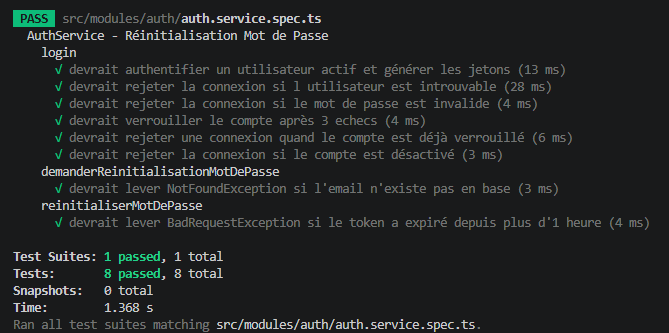
\includegraphics[width=\textwidth,keepaspectratio]
    {Images/test-unitaire-auth.png}
  \caption*{\small Auth}
\end{minipage}
\hfill
\begin{minipage}{0.48\textwidth}
  \centering
  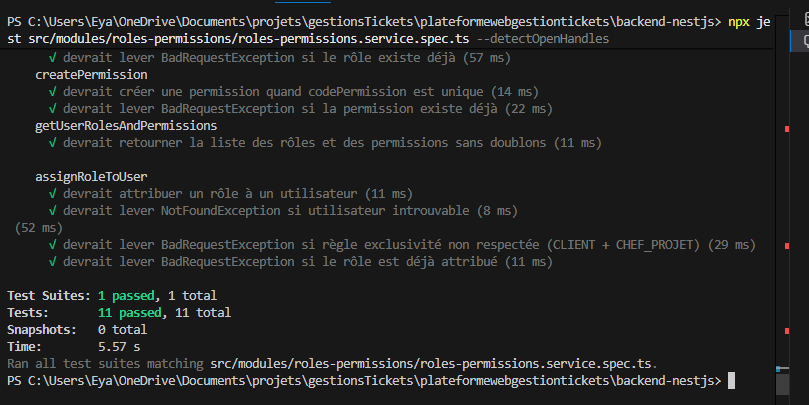
\includegraphics[width=\textwidth,keepaspectratio]
    {Images/test-sprint1-moduleRole+Permession.png}
  \caption*{\small RBAC}
\end{minipage}
\caption{Résultats des tests unitaires — Auth et RBAC}
\label{fig:test_unitaires}
\end{figure}

\begin{figure}[H]
\centering
\begin{minipage}{0.6\textwidth}
  \centering
  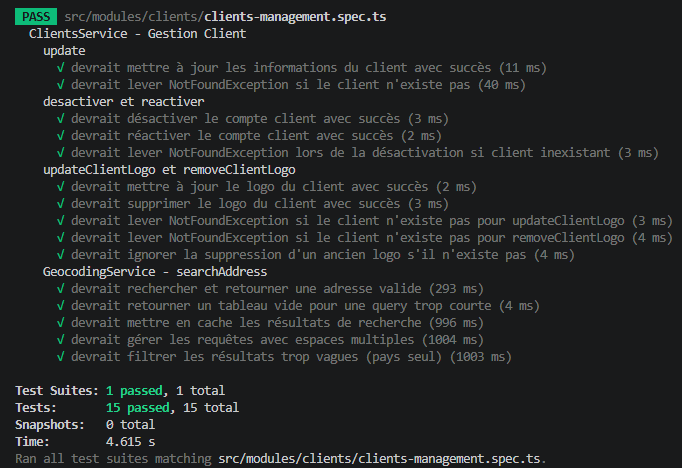
\includegraphics[width=\textwidth,keepaspectratio]
    {Images/test unit-ClientTestUnitaire.png}
  \caption*{\small Gestion des clients}
\end{minipage}
\caption{Résultats des tests unitaires — Gestion des clients}
\end{figure}

% \subsubsection{Tests de sécurité}
% \label{sec:tests_securite}

% Ces tests valident que les mécanismes de protection résistent aux accès
% non autorisés et aux tentatives d'attaque. Ils sont effectués via
% \textbf{Swagger} en combinaison avec les tests unitaires existants.

% \vspace{4pt}
% \noindent\textbf{4 tests exécutés — 4 réussis — 0 échec.}
% \vspace{6pt}

% \begin{itemize}[leftmargin=0pt]

% \item[$\square$] \textbf{Contrôle d'accès aux endpoints protégés}
% \hfill\textit{Guard \texttt{JwtAuthGuard} · \texttt{PermissionsGuard}}

% \begin{itemize}[label=$\bullet$, nosep, itemsep=1pt]
%   \item \texttt{GET /api/auth/me} sans token Bearer →
%     \textbf{401 Unauthorized}.
%   \item \texttt{GET /api/admin/users} avec token CLIENT →
%     \textbf{403 Forbidden}
%     (permission \texttt{users.read.all} absente).
%   \item \texttt{POST /api/admin/roles} avec token DEVELOPPEUR →
%     \textbf{403 Forbidden}
%     (permission \texttt{roles.create} absente).
%   \item Token JWT expiré (après 15 min) →
%     \textbf{401 Unauthorized}, rafraîchissement automatique déclenché
%     côté frontend (intercepteur Axios).
% \end{itemize}

% \vspace{6pt}
% \item[$\square$] \textbf{Protection contre le bruteforce}
% \hfill\textit{\texttt{maxLoginAttempts = 3} ·
% \texttt{lockDurationMs = 60\,000 ms}}

% \begin{itemize}[label=$\bullet$, nosep, itemsep=1pt]
%   \item \textbf{3 tentatives échouées} consécutives → champ
%     \texttt{compteVerrouilleJusquA} mis à jour en base, connexion
%     bloquée \textbf{1 minute}.
%   \item Tentative sur compte verrouillé avant expiration → rejetée
%     immédiatement, sans vérification du mot de passe.
% \end{itemize}

% \end{itemize}

% \begin{figure}[H]
% \centering
% \includegraphics[width=0.72\textwidth,keepaspectratio]
%   {Images/test-securite-acces.png}
% \caption{Tests de sécurité — Contrôle d'accès et protection bruteforce
%   via Swagger}
% \label{fig:test_securite}
% \end{figure}

\subsubsection{Tests d'intégration}
\label{sec:tests_integration}

Les tests d'intégration ont pour objectif de valider les échanges entre
les différentes couches de l'application (contrôleur, service et base de
données) en testant les endpoints REST dans leur ensemble. Ces tests sont
effectués via \textbf{Swagger UI} en soumettant des requêtes HTTP réelles
contre le backend en cours d'exécution, ce qui permet de vérifier le
comportement de l'API dans des conditions proches de la production.

\vspace{4pt}
\noindent\textbf{Bilan : 5 tests exécutés — 5 réussis — 0 échec.}
\vspace{6pt}

\begin{itemize}[leftmargin=0pt]

\item[$\square$] \textbf{Authentification}
\hfill\textit{Endpoint : \texttt{POST /api/auth/login}}

\noindent Cette suite valide le comportement complet de l'endpoint de
connexion, notamment le retour des jetons d'authentification, des rôles,
des permissions associées et la gestion des codes d'erreur HTTP selon les
différents cas d'entrée. Les cas suivants ont été couverts :

\begin{itemize}[label=$\bullet$, nosep, itemsep=2pt]
  \item Un utilisateur actif de rôle \texttt{ADMIN} fournit des
    identifiants valides : l'endpoint retourne le code \textbf{200 OK}
    accompagné des champs \texttt{accessToken}, \texttt{refreshToken},
    des données de l'utilisateur, de ses rôles et de la liste complète
    de ses permissions.
  \item L'adresse e-mail fournie n'existe pas en base de données :
    l'endpoint retourne le code \textbf{401 Unauthorized}.
  \item Le mot de passe fourni est incorrect : l'endpoint retourne le
    code \textbf{401 Unauthorized}.
  \item Les données soumises sont invalides (adresse e-mail mal formatée
    ou champ obligatoire vide) : l'endpoint retourne le code
    \textbf{400 Bad Request} accompagné d'un message de validation
    généré par \texttt{class-validator}.
  \item Le compte de l'utilisateur est désactivé
    (\texttt{estActif = false}) : l'endpoint retourne le code
    \textbf{401 Unauthorized} avec le message
    « Ce compte est désactivé ».
\end{itemize}

\end{itemize}

\begin{figure}[H]
\centering
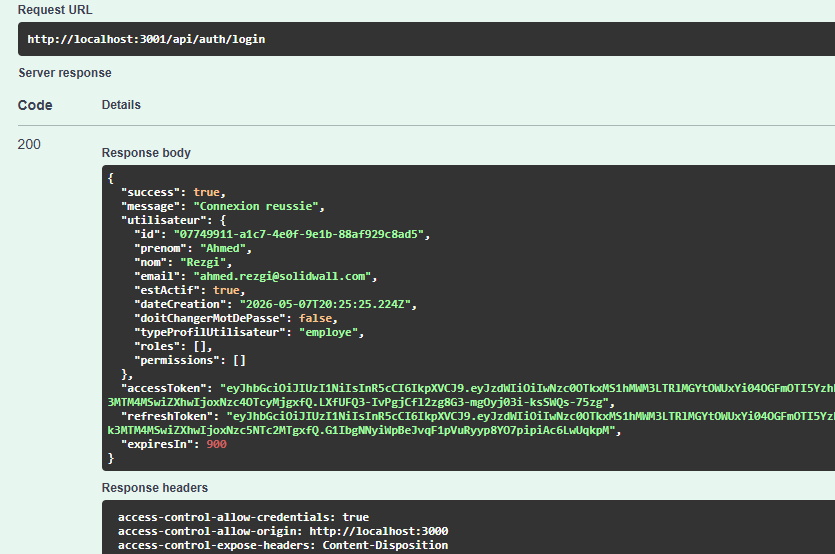
\includegraphics[width=0.60\textwidth,keepaspectratio]
  {Images/test-interg-login.png}
\caption{Test d'intégration — endpoint \texttt{POST /api/auth/login}
  via Swagger}
\label{fig:test_integration}
\end{figure}

%─────────────────────────────────────────────────────────────────────────────
\newpage
%─────────────────────────────────────────────────────────────────────────────
\subsubsection{Tests End-to-End}
\label{sec:tests_e2e}

Les tests End-to-End ont pour objectif de simuler les parcours utilisateurs
complets dans un navigateur réel piloté par \textbf{Playwright}. Ces tests
s'exécutent en interaction avec le frontend Next.js, le backend NestJS et
la base de données PostgreSQL, reproduisant ainsi les conditions réelles
d'utilisation de la plateforme.

\vspace{4pt}
\noindent\textbf{Bilan : 11 tests exécutés — 11 réussis — 0 échec.}
\vspace{6pt}

\begin{itemize}[leftmargin=0pt]

% ── 1. Authentification ───────────────────────────────────────────────────────
\item[$\square$] \textbf{Authentification}
\hfill\textit{10 scénarios : connexion classique, OAuth, déconnexion}

\noindent Cette suite valide le flux complet d'authentification en
simulant les actions réelles d'un utilisateur sur l'interface. Les cas
suivants ont été couverts :

\begin{itemize}[label=$\bullet$, nosep, itemsep=2pt]
  \item La page de connexion est chargée : le formulaire et les boutons
    d'authentification OAuth sont affichés correctement.
  \item Les champs du formulaire sont vides ou partiellement remplis :
    le bouton de soumission reste désactivé.
  \item L'utilisateur soumet des identifiants valides : le flux aboutit
    à une redirection vers la page d'accueil et une session est créée.
  \item L'utilisateur saisit un identifiant ou un mot de passe invalide :
    un message d'erreur approprié est affiché sans redirection.
  \item L'utilisateur échoue l'authentification \textbf{3 fois
    consécutives} : le compte est verrouillé pendant \textbf{1 minute}
    et un message d'information est affiché.
  \item L'utilisateur se déconnecte : les jetons sont supprimés du
    \texttt{localStorage} et l'utilisateur est redirigé vers la page
    \texttt{/connexion}.
  \item L'utilisateur s'authentifie via \textbf{Google} avec succès :
    les données du profil sont récupérées et une session valide est
    créée.
  \item L'authentification via \textbf{Google} échoue : un message
    d'erreur technique est affiché.
  \item L'utilisateur s'authentifie via \textbf{GitHub} avec succès :
    les données du profil sont récupérées et une session valide est
    créée.
  \item L'authentification via \textbf{GitHub} échoue : un message
    d'erreur technique est affiché.
\end{itemize}

\begin{figure}[H]
\centering
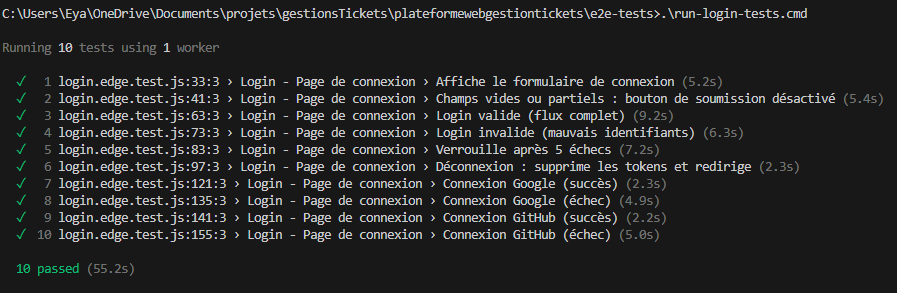
\includegraphics[width=0.68\textwidth,keepaspectratio]
  {Images/ExecDeTestCasesReussi-auth.png}
\caption{Tests End-to-End — Authentification via Playwright}
\label{fig:test_e2e_auth}
\end{figure}

% ── 2. Désactivation utilisateur ─────────────────────────────────────────────
\item[$\square$] \textbf{Gestion des utilisateurs}
\hfill\textit{1 scénario : désactivation avec réassignation des tickets}

\noindent Cette suite valide le flux complet de désactivation d'un
utilisateur disposant de tickets actifs, en simulant les actions réelles
d'un administrateur. Le cas suivant a été couvert :

\begin{itemize}[label=$\bullet$, nosep, itemsep=2pt]
  \item L'administrateur tente de désactiver un utilisateur actif
    disposant de \textbf{9 tickets actifs} (statuts \texttt{OUVERT},
    \texttt{EN\_COURS} ou \texttt{EN\_REVUE}) : le système affiche le
    modal de réassignation présentant la liste des développeurs
    disponibles \textbf{triés par charge de travail croissante}.
    L'administrateur procède à la réassignation de chaque ticket, puis
    confirme l'opération via le bouton « Réassigner et Désactiver ».
    Le système effectue les réassignations dans une transaction atomique,
    désactive le compte et envoie un e-mail de notification à
    l'utilisateur concerné.
\end{itemize}

\begin{figure}[H]
\centering
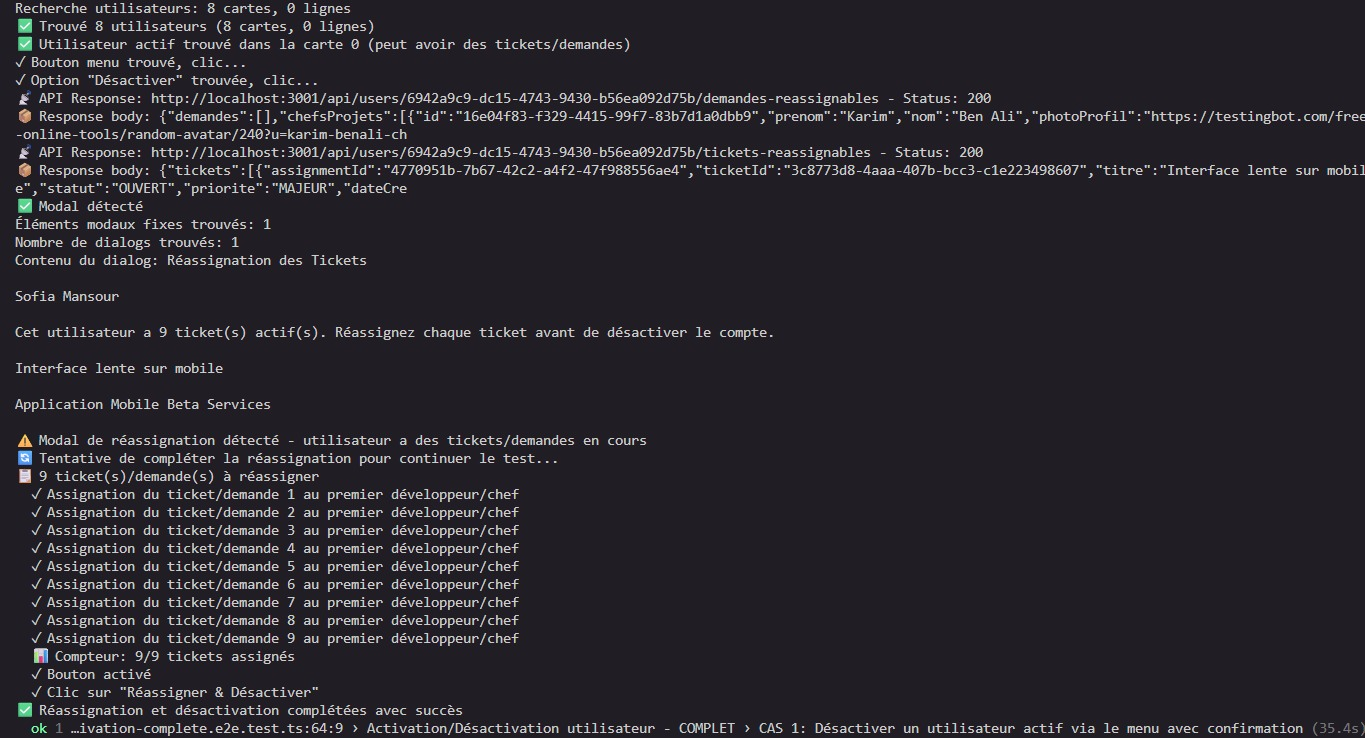
\includegraphics[width=0.68\textwidth,keepaspectratio]
  {Images/Test e2e desactiver utilisateu.png}
\caption{Tests End-to-End — Désactivation utilisateur via Playwright}
\label{fig:test_e2e_desactiver}
\end{figure}

\end{itemize}


% ---- Chapitre 6 ----
\hiddenpart{Sprint 4 -- Collaboration et Dashboards}
\chaptercover{6}{Sprint 4 -- Collaboration et Dashboards}
\section*{Introduction}

Ce chapitre présente le quatrième et dernier sprint du projet \textbf{SolidMaint}. Les sprints précédents nous ont permis de mettre en place les principales fonctionnalités du système : la gestion des utilisateurs, des clients, des contrats, ainsi que le traitement des demandes et des tickets. Ce sprint vient compléter la plateforme avec des fonctionnalités de collaboration et de suivi qui étaient encore manquantes.
\newline
Dans ce chapitre, nous présentons donc les fonctionnalités développées durant ce dernier sprint, à savoir : un module de suivi de l'activité avec un calendrier et des tableaux de bord, un système de messagerie interne, un espace de gestion des documents, et un centre de notifications pour que chaque utilisateur soit alerté dès qu'un événement le concerne.


% ─────────────────────────────────────────────────────────────────────────────
% SECTION 1 : SPRINT PLANNING MEETING
% ─────────────────────────────────────────────────────────────────────────────

\section{Sprint Planning Meeting}
La réunion de planification du quatrième sprint nous a permis de définir les objectifs à atteindre durant les trois dernières semaines de développement. Nous avons sélectionné les user stories prioritaires correspondant aux fonctionnalités de collaboration, de suivi et de communication, et nous avons estimé l'effort nécessaire pour chacune d'elles. Cette étape est déterminante pour garantir que l'ensemble de l'équipe partage une vision commune du travail à accomplir et que les livrables finaux répondent aux exigences exprimées dans le product backlog.

\subsection{Objectif du Sprint}

L'objectif principal de ce sprint est de finaliser la plateforme en offrant aux utilisateurs des outils de suivi, de communication et de gestion documentaire efficaces. Il s'agit concrètement de mettre en place un calendrier interactif permettant de visualiser les tickets et les demandes d'intervention dans le temps, d'intégrer des tableaux de bord personnalisés par rôle pour piloter l'activité et générer des rapports périodiques, de déployer un module de messagerie interne en temps réel facilitant la collaboration entre les membres de l'équipe au sein de canaux dédiés, de proposer un espace documentaire centralisé avec gestion des versions et traçabilité des consultations, et enfin de mettre en place un système de notifications multicanaux in-app, email, push navigateur et Slack afin que chaque acteur reçoive les informations pertinentes au moment opportun.

\subsubsection{Backlog du quatrième sprint}
\label{sec:backlog_sprint4}

Le tableau ci-dessous présente le Sprint Backlog détaillé avec les descriptions techniques et l'effort estimé pour chaque user story.

\textbf{1 : Effort faible, 2 : Effort moyen, 3 : Effort élevé}
\newpage
\rowcolors{0}{}{}
\arrayrulecolor{black}
\renewcommand{\arraystretch}{1.3}
\setlength{\extrarowheight}{3pt}
\small
\sloppy
\begin{longtable}{|C{1cm}|L{6.5cm}|L{7cm}|C{1cm}|}
\caption{Backlog du sprint 4}\label{tab:backlog_sprint4}\\
\hline
\textbf{ID US} & \textbf{User Story} & \textbf{Description technique} & \textbf{Effort} \\
\hline
\endfirsthead

\hline
\textbf{ID US} & \textbf{User Story} & \textbf{Description technique} & \textbf{Effort} \\
\hline
\endhead

\hline
\endfoot

\hline
\endlastfoot

% Epic 13: Calendrier et planification
\multicolumn{4}{|l|}{\cellcolor{blue!20}\textbf{Epic 13 - Calendrier et planification}} \\
\hline

US66 & En tant qu'\textbf{utilisateur}, je souhaite visualiser les tickets et demandes de maintenance sur un calendrier mensuel afin d'avoir une vue globale des interventions. &
\begin{itemize}[nosep, left=0pt, label={$\bullet$}]
\item Mettre en place la page calendrier côté Next.js
\item S'appuyer sur une vue mois et une vue agenda/Gantt
\item Agréger les tickets, demandes et données de charge existantes
\item Colorer les événements selon leur type et leur statut
\item Permettre la navigation mois par mois et la consultation mobile
\end{itemize} & 3 \\
\hline

US67 & En tant qu'\textbf{administrateur}, je souhaite identifier visuellement les urgences SLA sur le calendrier afin de prioriser les interventions critiques. &
\begin{itemize}[nosep, left=0pt, label={$\bullet$}]
\item Calculer l'urgence à partir des échéances SLA des tickets
\item Mettre en évidence les tickets en retard ou proches de l'échéance
\item Utiliser une coloration visuelle et des badges d'alerte
\item Ajouter une légende explicative dans l'interface
\item Réutiliser les informations SLA déjà calculées côté backend
\end{itemize} & 2 \\
\hline

US68 & En tant que \textbf{chef de projet}, je souhaite accéder à une vue Gantt / Agenda afin d'analyser la charge de travail et la progression de chaque développeur. &
\begin{itemize}[nosep, left=0pt, label={$\bullet$}]
\item Intégrer la vue agenda/Gantt dans la page calendrier
\item Développer une visualisation de la charge par développeur
\item S'appuyer sur les endpoints existants de suivi de charge et de planning
\item Afficher la timeline des tickets assignés
\item Ajouter un filtre par développeur, projet et période
\end{itemize} & 3 \\
\hline

US69 & En tant qu'\textbf{utilisateur}, je souhaite accéder aux détails d'un ticket directement depuis le calendrier afin de consulter ou modifier l'intervention rapidement. &
\begin{itemize}[nosep, left=0pt, label={$\bullet$}]
\item Rendre les événements du calendrier cliquables
\item Ouvrir un panneau latéral ou rediriger vers la fiche ticket
\item Afficher le statut, la priorité, l'assignation et l'échéance
\item Permettre l'accès rapide à la vue complète du ticket
\end{itemize} & 2 \\
\hline

% Epic 10: Messagerie et collaboration
\multicolumn{4}{|l|}{\cellcolor{blue!20}\textbf{Epic 10 - Messagerie et collaboration}} \\
\hline

US70 & En tant qu'\textbf{utilisateur}, je souhaite accéder à une messagerie intégrée afin de communiquer avec mon équipe. &
\begin{itemize}[nosep, left=0pt, label={$\bullet$}]
\item Mettre en place les channels de discussion côté backend et frontend
\item Différencier les channels généraux, projets, tickets, demandes et privés
\item Utiliser les WebSockets pour la diffusion en temps réel
\item Créer l'interface de messagerie côté Next.js
\item Afficher les canaux, les membres et les messages non lus
\end{itemize} & 3 \\
\hline

US71 & En tant qu'\textbf{utilisateur}, je souhaite envoyer des messages dans un channel afin de communiquer. &
\begin{itemize}[nosep, left=0pt, label={$\bullet$}]
\item Développer l'endpoint \texttt{POST /api/messages/channel/:channelId}
\item Enregistrer les messages avec horodatage et auteur
\item Diffuser le message en temps réel via WebSocket
\item Afficher l'historique des messages du channel
\item Gérer les messages avec pièces jointes via un endpoint dédié
\end{itemize} & 2 \\
\hline

US72 & En tant qu'\textbf{utilisateur}, je souhaite répondre à un message afin de créer un fil de discussion. &
\begin{itemize}[nosep, left=0pt, label={$\bullet$}]
\item S'appuyer sur le champ \texttt{parentMessageId} dans le message
\item Regrouper les réponses en fil de discussion dans l'interface
\item Notifier les participants concernés dans le thread
\item Permettre le repli et le dépli des discussions
\end{itemize} & 2 \\
\hline

US73 & En tant qu'\textbf{utilisateur}, je souhaite mentionner des collègues afin d'attirer leur attention. &
\begin{itemize}[nosep, left=0pt, label={$\bullet$}]
\item Mettre en place l'autocomplétion des utilisateurs dans l'éditeur
\item Rechercher les utilisateurs pour la suggestion des mentions
\item Notifier les utilisateurs mentionnés via in-app et email
\item Mettre en évidence les messages contenant des mentions
\end{itemize} & 2 \\
\hline

US74 & En tant qu'\textbf{utilisateur}, je souhaite éditer mes messages afin de corriger des erreurs. &
\begin{itemize}[nosep, left=0pt, label={$\bullet$}]
\item Développer l'endpoint \texttt{PATCH /api/messages/:messageId}
\item Autoriser l'édition uniquement par l'auteur du message
\item Limiter l'édition à une fenêtre temporelle courte
\item Conserver l'historique des modifications
\item Afficher un indicateur de modification
\end{itemize} & 1 \\
\hline

US75 & En tant qu'\textbf{utilisateur}, je souhaite supprimer mes messages afin de retirer du contenu inapproprié. &
\begin{itemize}[nosep, left=0pt, label={$\bullet$}]
\item Développer l'endpoint \texttt{DELETE /api/messages/:messageId}
\item Confirmer l'action avant suppression
\item Conserver la suppression sous forme de soft delete
\item Préserver l'audit et l'historique si nécessaire
\end{itemize} & 1 \\
\hline

US76 & En tant qu'\textbf{utilisateur}, je souhaite épingler des messages importants afin de les retrouver facilement. &
\begin{itemize}[nosep, left=0pt, label={$\bullet$}]
\item Développer l'endpoint \texttt{POST /api/messages/:messageId/pin}
\item Afficher les messages épinglés en haut du channel
\item Ajouter une icône d'épingle sur le message
\item Restreindre cette action selon le rôle dans le channel
\end{itemize} & 1 \\
\hline

US77 & En tant que \textbf{chef de projet}, je souhaite voir qui est en ligne dans mon équipe afin de savoir qui je peux solliciter. &
\begin{itemize}[nosep, left=0pt, label={$\bullet$}]
\item Utiliser le suivi de dernière connexion et les événements temps réel
\item Afficher le statut de présence dans les listes d'utilisateurs
\item Mettre en évidence les membres récemment actifs
\item Présenter les dernières activités dans l'interface
\end{itemize} & 2 \\
\hline

US78 & En tant qu'\textbf{utilisateur}, je souhaite voir qui est en ligne afin de savoir qui est disponible. &
\begin{itemize}[nosep, left=0pt, label={$\bullet$}]
\item Afficher les statuts de présence dans les composants de messagerie
\item Synchroniser l'état via les événements temps réel
\item Montrer la dernière activité ou la dernière connexion
\item Adapter l'affichage selon le rôle et le contexte
\end{itemize} & 2 \\
\hline

% Epic 11: Gestion des documents
\multicolumn{4}{|l|}{\cellcolor{blue!20}\textbf{Epic 11 - Gestion des documents}} \\
\hline

US79 & En tant qu'\textbf{utilisateur}, je souhaite uploader des documents afin de centraliser les fichiers. &
\begin{itemize}[nosep, left=0pt, label={$\bullet$}]
\item Développer l'endpoint \texttt{POST /api/documents/upload}
\item Autoriser jusqu'à 5 fichiers par envoi
\item Limiter la taille à 10 MB par fichier
\item Stocker les fichiers localement dans le répertoire documents
\item Associer les documents à un ticket ou à un contrat
\end{itemize} & 3 \\
\hline

US80 & En tant qu'\textbf{utilisateur}, je souhaite télécharger des documents afin de les consulter hors ligne. &
\begin{itemize}[nosep, left=0pt, label={$\bullet$}]
\item Prévoir le téléchargement à partir des fichiers stockés
\item Tracer la consultation des documents pour la traçabilité
\item Rattacher le document à son ticket ou contrat d'origine
\item Préparer l'ouverture dans le navigateur ou le téléchargement direct
\end{itemize} & 2 \\
\hline

US81 & En tant qu'\textbf{utilisateur}, je souhaite gérer les versions des documents afin d'assurer la traçabilité. &
\begin{itemize}[nosep, left=0pt, label={$\bullet$}]
\item Développer l'endpoint \texttt{GET /api/documents/:id/versions}
\item Développer l'endpoint \texttt{PATCH /api/documents/:id/replace}
\item Conserver les anciennes versions lors du remplacement
\item Exiger un commentaire lors du remplacement
\item Permettre l'accès à l'historique des versions
\end{itemize} & 2 \\
\hline

US82 & En tant qu'\textbf{utilisateur}, je souhaite consulter l'historique des consultations afin de voir qui a accédé au document. &
\begin{itemize}[nosep, left=0pt, label={$\bullet$}]
\item Développer l'endpoint \texttt{GET /api/documents/:id/consultations}
\item Afficher les consultations avec date, heure et utilisateur
\item Prévoir un filtre par période
\item Permettre l'exploitation de l'historique à des fins de traçabilité
\end{itemize} & 1 \\
\hline

US83 & En tant qu'\textbf{utilisateur}, je souhaite archiver des documents afin de nettoyer la vue active. &
\begin{itemize}[nosep, left=0pt, label={$\bullet$}]
\item Développer l'endpoint \texttt{PATCH /api/documents/:id/archive}
\item Développer l'endpoint \texttt{PATCH /api/documents/:id/restore}
\item Exclure les documents archivés de la vue courante
\item Réserver l'archivage à l'administrateur
\end{itemize} & 1 \\
\hline

US84 & En tant que \textbf{chef de projet}, je souhaite générer automatiquement un PV à partir d'un ticket afin de documenter les interventions. &
\begin{itemize}[nosep, left=0pt, label={$\bullet$}]
\item Générer un PDF à partir des informations du ticket
\item Inclure les actions réalisées, les intervenants et le temps passé
\item Enregistrer le PV comme document lié au ticket
\item Prévoir une exportation ou une signature selon le besoin métier
\end{itemize} & 3 \\
\hline

US85 & En tant que \textbf{client}, je souhaite télécharger les PV de mes tickets afin de conserver une trace des interventions. &
\begin{itemize}[nosep, left=0pt, label={$\bullet$}]
\item Exposer les PV liés aux tickets du client dans son espace
\item Permettre le téléchargement des PV générés
\item Notifier le client lors de la génération d'un nouveau PV
\item Rattacher le PV au contrat ou au ticket concerné
\end{itemize} & 1 \\
\hline

US86 & En tant que \textbf{développeur ou chef de projet}, je souhaite consulter la base de connaissances afin de trouver des solutions existantes. &
\begin{itemize}[nosep, left=0pt, label={$\bullet$}]
\item Mettre en place la recherche dans la base de connaissances
\item Filtrer par mots-clés, catégorie et tags
\item Afficher le titre, l'extrait et le score de pertinence
\item Ouvrir l'article complet en un clic
\end{itemize} & 2 \\
\hline

US87 & En tant qu'\textbf{administrateur}, je souhaite créer des articles de la base de connaissances afin d'enrichir la documentation. &
\begin{itemize}[nosep, left=0pt, label={$\bullet$}]
\item Développer l'endpoint de création d'articles KB
\item Utiliser un éditeur Markdown pour la rédaction
\item Ajouter des tags, une catégorie et un auteur
\item Permettre l'archivage des articles obsolètes
\end{itemize} & 2 \\
\hline

US88 & En tant qu'\textbf{utilisateur}, je souhaite créer une nouvelle version d'un document afin de maintenir l'historique. &
\begin{itemize}[nosep, left=0pt, label={$\bullet$}]
\item Réutiliser le mécanisme de remplacement de document
\item Conserver toutes les versions précédentes
\item Numéroter implicitement les versions dans l'historique
\item Exiger un commentaire pour documenter la nouvelle version
\end{itemize} & 2 \\
\hline

US89 & En tant qu'\textbf{utilisateur}, je souhaite comparer deux versions d'un document afin de voir les différences. &
\begin{itemize}[nosep, left=0pt, label={$\bullet$}]
\item Prévoir un endpoint ou un traitement de comparaison de versions
\item Afficher les deux versions côte à côte
\item Mettre en évidence les différences textuelles
\item Faciliter la revue des changements avant validation
\end{itemize} & 2 \\
\hline

US90 & En tant qu'\textbf{administrateur}, je souhaite voir qui a consulté un document afin de suivre sa diffusion. &
\begin{itemize}[nosep, left=0pt, label={$\bullet$}]
\item Exploiter l'historique des consultations de documents
\item Afficher les utilisateurs, dates et périodes de consultation
\item Prévoir une vue statistique pour l'administration
\item Permettre l'export des données si nécessaire
\end{itemize} & 2 \\
\hline

% Epic 12: Notifications
\multicolumn{4}{|l|}{\cellcolor{blue!20}\textbf{Epic 12 - Notifications et alertes}} \\
\hline

US91 & En tant qu'\textbf{utilisateur}, je souhaite recevoir des notifications in-app afin d'être informé en temps réel. &
\begin{itemize}[nosep, left=0pt, label={$\bullet$}]
\item Développer l'API de notification in-app
\item Afficher la liste paginée des notifications
\item Gérer le compteur de notifications non lues
\item Permettre le marquage lu et lu partout
\item Rendre les notifications cliquables
\end{itemize} & 2 \\
\hline

US92 & En tant qu'\textbf{utilisateur}, je souhaite recevoir des notifications par email afin d'être informé hors connexion. &
\begin{itemize}[nosep, left=0pt, label={$\bullet$}]
\item Configurer l'envoi d'emails transactionnels
\item S'appuyer sur une file de traitement asynchrone
\item Envoyer des emails pour les événements critiques
\item Prévoir la configuration de préférences de notification
\end{itemize} & 2 \\
\hline

US93 & En tant que \textbf{membre technique}, je souhaite recevoir des notifications Slack afin d'être alerté sur mon outil de travail. &
\begin{itemize}[nosep, left=0pt, label={$\bullet$}]
\item Intégrer un service de notification Slack
\item Envoyer des alertes pour les événements critiques
\item Prévoir la configuration des canaux selon le besoin métier
\item Compléter les notifications in-app et email
\end{itemize} & 2 \\
\hline

US94 & En tant qu'\textbf{utilisateur}, je souhaite recevoir des notifications push navigateur afin d'être alerté même hors onglet. &
\begin{itemize}[nosep, left=0pt, label={$\bullet$}]
\item Mettre en place les notifications push navigateur
\item Demander et gérer l'autorisation utilisateur
\item Envoyer des push pour les événements critiques
\item Ouvrir directement l'application lors du clic
\end{itemize} & 2 \\
\hline

US95 & En tant qu'\textbf{utilisateur}, je souhaite consulter l'historique de mes notifications afin de retrouver une information. &
\begin{itemize}[nosep, left=0pt, label={$\bullet$}]
\item Développer la liste paginée des notifications
\item Ajouter un filtre par statut lu ou non lu
\item Prévoir un filtre temporel dans l'interface
\item Permettre la recherche dans l'historique
\end{itemize} & 1 \\
\hline

% Epic 13: Dashboards et rapports
\multicolumn{4}{|l|}{\cellcolor{blue!20}\textbf{Epic 13 - Dashboards et rapports}} \\
\hline

US96 & En tant qu'\textbf{administrateur}, je souhaite consulter un dashboard global afin de piloter le système. &
\begin{itemize}[nosep, left=0pt, label={$\bullet$}]
\item Développer l'endpoint \texttt{GET /api/dashboard/stats}
\item Afficher les KPI globaux du système
\item Suivre les tickets, les contrats, les clients et la charge
\item Ajouter les alertes SLA et les tendances récentes
\end{itemize} & 3 \\
\hline

US97 & En tant que \textbf{chef de projet}, je souhaite consulter un dashboard d'équipe afin de piloter l'activité. &
\begin{itemize}[nosep, left=0pt, label={$\bullet$}]
\item Exploiter les données de tickets et de charge développeur
\item Afficher la répartition de la charge par membre
\item Suivre les retards, les urgences et les tickets bloqués
\item Prévoir une vue orientée pilotage d'équipe
\end{itemize} & 2 \\
\hline

US98 & En tant que \textbf{développeur}, je souhaite consulter mon dashboard personnel afin d'organiser ma journée. &
\begin{itemize}[nosep, left=0pt, label={$\bullet$}]
\item Développer l'endpoint \texttt{GET /api/tickets/dashboard/employee}
\item Afficher les tickets assignés avec priorité et échéance
\item Lister les urgences du jour
\item Suivre le temps de travail journalier
\item Identifier les échéances proches et les tickets en cours
\end{itemize} & 2 \\
\hline

US99 & En tant que \textbf{client}, je souhaite consulter mon dashboard afin de suivre mes projets. &
\begin{itemize}[nosep, left=0pt, label={$\bullet$}]
\item Développer l'endpoint \texttt{GET /api/dashboard/client}
\item Afficher les contrats actifs et leur état
\item Suivre les demandes et tickets ouverts
\item Présenter les documents et informations utiles au client
\end{itemize} & 2 \\
\hline

US100 & En tant qu'\textbf{administrateur}, je souhaite générer un rapport d'activité mensuel afin de présenter les statistiques. &
\begin{itemize}[nosep, left=0pt, label={$\bullet$}]
\item Développer l'endpoint \texttt{GET /api/dashboard/rapport-mensuel}
\item Calculer les tickets traités, le temps passé et le respect SLA
\item Prévoir l'export PDF et Excel côté interface
\item Ajouter des graphiques pour la présentation des résultats
\end{itemize} & 3 \\
\hline

US101 & En tant qu'\textbf{administrateur}, je souhaite générer des rapports de conformité SLA afin de justifier les performances. &
\begin{itemize}[nosep, left=0pt, label={$\bullet$}]
\item Exploiter les indicateurs SLA du dashboard admin
\item Calculer le taux de conformité par période ou par contrat
\item Identifier les tickets en dépassement
\item Prévoir un export de rapport pour la justification métier
\end{itemize} & 2 \\
\hline

US102 & En tant que \textbf{chef de projet}, je souhaite générer des rapports d'activité afin de présenter l'avancement. &
\begin{itemize}[nosep, left=0pt, label={$\bullet$}]
\item Agréger les données de tickets et de charge d'équipe
\item Afficher l'évolution de l'activité par période
\item Comparer les tickets créés, traités et en retard
\item Prévoir un export PDF ou Excel selon le besoin
\end{itemize} & 2 \\
\hline

\end{longtable}

\newpage

% ─────────────────────────────────────────────────────────────────────────────
% SECTION 2 : ANALYSE
% ─────────────────────────────────────────────────────────────────────────────

\section{Analyse}
Dans le cadre de ce sprint, l'analyse fonctionnelle a consisté à formaliser les interactions entre les différents acteurs et les modules métiers de la solution. Cette étape a permis de traduire les besoins exprimés dans le backlog en cas d'utilisation concrets, en tenant compte des contraintes de temps réel, de traçabilité, de sécurité et de personnalisation par rôle.

\label{sec:analyse_sprint4}

\subsection{Diagramme de cas d'utilisation du quatrième sprint}
La figure ci-dessous présente le diagramme de cas d'utilisation du quatrième sprint.

\begin{figure}[H]
    \centering
    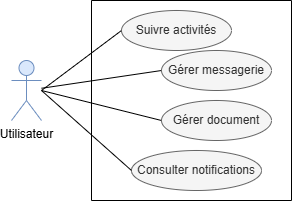
\includegraphics[width=0.70\textwidth,height=0.50\textheight,keepaspectratio]{Images/Diagramme cas utilisation sprint 4.png}
    \caption{Diagramme de cas d'utilisation du quatrième sprint}
    \label{fig:use_case_sprint4}
\end{figure}

Nous allons accompagner les cas d'utilisation d'un texte descriptif pour expliquer le scénario de chaque cas ainsi que ses exceptions.

% ──────────────────────────────────────────────────────
\subsection{Analyse de la fonctionnalité « Suivre Activité »}
Dans cette partie, nous allons présenter les cas d'utilisation relatifs au suivi de l'activité afin de comprendre les principales fonctionnalités du système, ce qui permet d'avoir une vue globale des interactions.

\subsubsection{Raffinement du cas d'utilisation « Suivre Activité »}
Au cours de cette partie, nous allons analyser chaque cas d'utilisation raffiné pour le suivi de l'activité :

\begin{figure}[H]
  \centering
  %\includegraphics[width=0.85\textwidth,height=0.75\textheight,keepaspectratio]{Images/suivre_activite.png}
  \caption{Raffinement du cas d'utilisation « Suivre Activité »}
  \label{fig:suivre_activite}
\end{figure}

\subsubsection{Description textuelle du cas d'utilisation « Consulter calendrier »}
La figure ci-dessous présente la description textuelle du cas d'utilisation « Consulter calendrier ».

\footnotesize
\renewcommand{\arraystretch}{0.95}
\begin{longtable}{|P{3.5cm}|P{10.5cm}|}
\hline
\endfirsthead
\hline
\endhead
\hline
\endfoot
\hline
\endlastfoot
\textbf{Nom du cas d'utilisation} & Consulter calendrier \\
\hline
\textbf{Acteurs} & Administrateur, Chef de projet, Développeur, Client \\
\hline
\textbf{Précondition} & L'utilisateur est authentifié et dispose de la permission d'accès au module calendrier. \\
\hline
\textbf{Postcondition} & Les tickets et demandes de maintenance sont affichés sur le calendrier selon le filtre choisi. \\
\hline
\textbf{Scénario nominal} &
\begin{minipage}[t]{\linewidth}\raggedright
\begin{enumerate}[label=\arabic*., nosep,leftmargin=0.6cm,topsep=0pt,itemsep=1pt]
\item L'utilisateur accède à la page « Calendrier » depuis le menu principal.
\item Le système récupère la liste des tickets et des demandes associés à l'utilisateur via l'API.
\item Le système affiche les éléments dans une vue mensuelle avec un code couleur par type d'élément.
\item L'utilisateur sélectionne une vue (mensuelle ou agenda) selon ses besoins.
\item L'utilisateur clique sur un élément pour accéder à sa fiche détaillée.
\end{enumerate}
\end{minipage} \\
\hline
\textbf{Scénario alternatif} &
\begin{minipage}[t]{\linewidth}\raggedright
\begin{enumerate}[label=A\arabic*.,nosep,leftmargin=0.6cm,topsep=0pt,itemsep=1pt]
\item Le chef de projet bascule vers la vue Gantt pour analyser la charge par développeur et la progression des tickets par période.
\item L'utilisateur applique un filtre temporel (jour, semaine, mois) pour affiner la période affichée.
\item Le système détecte des tickets critiques ou des échéances SLA dépassées et les met en évidence visuellement avec une légende de priorité.
\end{enumerate}
\end{minipage} \\
\hline
\textbf{Scénario d'exception} &
\begin{minipage}[t]{\linewidth}\raggedright
\begin{enumerate}[label=E\arabic*.,nosep,leftmargin=0.6cm,topsep=0pt,itemsep=1pt]
\item Une erreur de communication avec l'API survient lors du chargement des données ; le système affiche un message d'erreur et propose de recharger la page.
\end{enumerate}
\end{minipage} \\
\hline
\end{longtable}
\captionof{table}{Description textuelle du cas d'utilisation « Consulter calendrier »}
\normalsize

\subsubsection{Description textuelle du cas d'utilisation « Consulter dashboard »}
La figure ci-dessous présente la description textuelle du cas d'utilisation « Consulter dashboard ».

\footnotesize
\renewcommand{\arraystretch}{0.95}
\begin{longtable}{|P{3.5cm}|P{10.5cm}|}
\hline
\endfirsthead
\hline
\endhead
\hline
\endfoot
\hline
\endlastfoot
\textbf{Nom du cas d'utilisation} & Consulter dashboard \\
\hline
\textbf{Acteurs} & Administrateur, Chef de projet, Client \\
\hline
\textbf{Précondition} & L'utilisateur est authentifié. Le système dispose de données d'activité enregistrées. \\
\hline
\textbf{Postcondition} & Les indicateurs clés sont affichés selon le rôle de l'utilisateur connecté. \\
\hline
\textbf{Scénario nominal} &
\begin{minipage}[t]{\linewidth}\raggedright
\begin{enumerate}[label=\arabic*., nosep,leftmargin=0.6cm,topsep=0pt,itemsep=1pt]
\item L'utilisateur accède à la page « Dashboard » depuis le menu principal.
\item Le système identifie le rôle de l'utilisateur et charge les indicateurs correspondants.
\item L'administrateur visualise les statistiques globales, les tendances, les alertes et le classement des développeurs les plus actifs.
\item Le chef de projet consulte les KPI de son équipe, les demandes en attente, les tickets SLA critiques et la charge de travail de ses développeurs.
\item Le client accède à une vue synthétique de ses projets, contrats et tickets en cours.
\end{enumerate}
\end{minipage} \\
\hline
\textbf{Scénario alternatif} &
\begin{minipage}[t]{\linewidth}\raggedright
\begin{enumerate}[label=A\arabic*.,nosep,leftmargin=0.6cm,topsep=0pt,itemsep=1pt]
\item L'administrateur sélectionne un mois et une année pour générer et afficher un rapport mensuel d'activité.
\item Le chef de projet filtre les données par projet ou par période pour obtenir un rapport d'avancement ciblé.
\end{enumerate}
\end{minipage} \\
\hline
\textbf{Scénario d'exception} &
\begin{minipage}[t]{\linewidth}\raggedright
\begin{enumerate}[label=E\arabic*.,nosep,leftmargin=0.6cm,topsep=0pt,itemsep=1pt]
\item Aucune donnée d'activité n'est disponible pour la période sélectionnée ; le système affiche un message indiquant l'absence de données et invite l'utilisateur à élargir la période.
\end{enumerate}
\end{minipage} \\
\hline
\end{longtable}
\captionof{table}{Description textuelle du cas d'utilisation « Consulter dashboard »}
\normalsize

% ──────────────────────────────────────────────────────
\subsection{Analyse de la fonctionnalité « Gérer Messagerie »}
Dans cette partie, nous allons présenter les cas d'utilisation relatifs à la gestion de la messagerie afin de comprendre les principales fonctionnalités du système de communication interne, ce qui permet d'avoir une vue globale des interactions en temps réel.

\subsubsection{Raffinement du cas d'utilisation « Gérer Messagerie »}
Au cours de cette partie, nous allons analyser chaque cas d'utilisation raffiné pour la gestion de la messagerie :

\begin{figure}[H]
  \centering
  %\includegraphics[width=0.85\textwidth,height=0.75\textheight,keepaspectratio]{Images/gerer_messagerie.png}
  \caption{Raffinement du cas d'utilisation « Gérer Messagerie »}
  \label{fig:gerer_messagerie}
\end{figure}

\subsubsection{Description textuelle du cas d'utilisation « Envoyer message »}
La figure ci-dessous présente la description textuelle du cas d'utilisation « Envoyer message ».

\footnotesize
\renewcommand{\arraystretch}{0.95}
\begin{longtable}{|P{3.5cm}|P{10.5cm}|}
\hline
\endfirsthead
\hline
\endhead
\hline
\endfoot
\hline
\endlastfoot
\textbf{Nom du cas d'utilisation} & Envoyer message \\
\hline
\textbf{Acteurs} & Administrateur, Chef de projet, Développeur, Client \\
\hline
\textbf{Précondition} & L'utilisateur est authentifié et a accès à au moins un canal de messagerie. \\
\hline
\textbf{Postcondition} & Le message est enregistré et diffusé en temps réel à tous les membres du canal concerné. \\
\hline
\textbf{Scénario nominal} &
\begin{minipage}[t]{\linewidth}\raggedright
\begin{enumerate}[label=\arabic*., nosep,leftmargin=0.6cm,topsep=0pt,itemsep=1pt]
\item L'utilisateur accède au module de messagerie et sélectionne un canal dans la liste de ses canaux.
\item Le système charge l'historique des messages du canal sélectionné.
\item L'utilisateur saisit son message dans le champ de saisie et valide l'envoi.
\item Le système enregistre le message et le diffuse instantanément à tous les membres du canal via la connexion WebSocket.
\item Le message apparaît dans le fil de discussion en temps réel pour tous les participants connectés.
\end{enumerate}
\end{minipage} \\
\hline
\textbf{Scénario alternatif} &
\begin{minipage}[t]{\linewidth}\raggedright
\begin{enumerate}[label=A\arabic*.,nosep,leftmargin=0.6cm,topsep=0pt,itemsep=1pt]
\item L'utilisateur joint un ou plusieurs fichiers à son message ; le système les envoie simultanément avec le contenu textuel.
\item L'utilisateur mentionne un collègue dans son message en utilisant le symbole @ ; le système identifie la mention et notifie le membre concerné.
\item L'utilisateur répond à un message existant ; le système crée une réponse liée au message parent et affiche le fil de discussion associé.
\end{enumerate}
\end{minipage} \\
\hline
\textbf{Scénario d'exception} &
\begin{minipage}[t]{\linewidth}\raggedright
\begin{enumerate}[label=E\arabic*.,nosep,leftmargin=0.6cm,topsep=0pt,itemsep=1pt]
\item La connexion WebSocket est interrompue lors de l'envoi ; le système affiche une erreur de connexion et invite l'utilisateur à réessayer après rétablissement de la connexion.
\item L'utilisateur n'est plus membre du canal au moment de l'envoi (suppression concurrente de ses droits) ; le serveur rejette le message et le système signale l'absence d'autorisation.
\end{enumerate}
\end{minipage} \\
\hline
\end{longtable}
\captionof{table}{Description textuelle du cas d'utilisation « Envoyer message »}
\normalsize

\subsubsection{Description textuelle du cas d'utilisation « Gérer message »}
La figure ci-dessous présente la description textuelle du cas d'utilisation « Gérer message ».

\footnotesize
\renewcommand{\arraystretch}{0.95}
\begin{longtable}{|P{3.5cm}|P{10.5cm}|}
\hline
\endfirsthead
\hline
\endhead
\hline
\endfoot
\hline
\endlastfoot
\textbf{Nom du cas d'utilisation} & Gérer message \\
\hline
\textbf{Acteurs} & Utilisateur (auteur du message) \\
\hline
\textbf{Précondition} & L'utilisateur est authentifié et est l'auteur du message concerné. \\
\hline
\textbf{Postcondition} & Le message est modifié ou supprimé, et les membres du canal voient la mise à jour en temps réel. \\
\hline
\textbf{Scénario nominal} &
\begin{minipage}[t]{\linewidth}\raggedright
\begin{enumerate}[label=\arabic*., nosep,leftmargin=0.6cm,topsep=0pt,itemsep=1pt]
\item L'utilisateur localise son message dans le fil de discussion et actionne le menu d'options.
\item Il choisit l'action « Modifier » et corrige le contenu dans le champ d'édition.
\item Il valide la modification.
\item Le système enregistre la nouvelle version du message et diffuse la mise à jour en temps réel à tous les membres du canal.
\end{enumerate}
\end{minipage} \\
\hline
\textbf{Scénario alternatif} &
\begin{minipage}[t]{\linewidth}\raggedright
\begin{enumerate}[label=A\arabic*.,nosep,leftmargin=0.6cm,topsep=0pt,itemsep=1pt]
\item L'utilisateur choisit de supprimer son message ; le système retire le contenu du fil tout en maintenant la cohérence des réponses liées et notifie les membres du canal en temps réel.
\item L'utilisateur épingle un message important dans le canal ; le message apparaît dans la section des messages épinglés, accessible à tous les membres.
\end{enumerate}
\end{minipage} \\
\hline
\textbf{Scénario d'exception} &
\begin{minipage}[t]{\linewidth}\raggedright
\begin{enumerate}[label=E\arabic*.,nosep,leftmargin=0.6cm,topsep=0pt,itemsep=1pt]
\item Le message a été supprimé par un administrateur entre le moment où l'utilisateur a ouvert le menu et celui où il valide la modification ; le serveur lève une exception et informe l'utilisateur que l'opération est impossible.
\end{enumerate}
\end{minipage} \\
\hline
\end{longtable}
\captionof{table}{Description textuelle du cas d'utilisation « Gérer message »}
\normalsize

% ──────────────────────────────────────────────────────
\subsection{Analyse de la fonctionnalité « Gérer Documents »}
Dans cette partie, nous allons présenter les cas d'utilisation relatifs à la gestion des documents afin de comprendre les principales fonctionnalités du module documentaire, ce qui permet d'avoir une vue globale des interactions.

\subsubsection{Raffinement du cas d'utilisation « Gérer Documents »}
Au cours de cette partie, nous allons analyser chaque cas d'utilisation raffiné pour la gestion des documents :

\begin{figure}[H]
  \centering
  %\includegraphics[width=0.85\textwidth,height=0.75\textheight,keepaspectratio]{Images/gerer_documents.png}
  \caption{Raffinement du cas d'utilisation « Gérer Documents »}
  \label{fig:gerer_documents}
\end{figure}

\subsubsection{Description textuelle du cas d'utilisation « Déposer document »}
La figure ci-dessous présente la description textuelle du cas d'utilisation « Déposer document ».

\footnotesize
\renewcommand{\arraystretch}{0.95}
\begin{longtable}{|P{3.5cm}|P{10.5cm}|}
\hline
\endfirsthead
\hline
\endhead
\hline
\endfoot
\hline
\endlastfoot
\textbf{Nom du cas d'utilisation} & Déposer document \\
\hline
\textbf{Acteurs} & Administrateur, Chef de projet, Développeur, Client \\
\hline
\textbf{Précondition} & L'utilisateur est authentifié et dispose des droits d'accès au ticket ou au contrat auquel le document doit être rattaché. \\
\hline
\textbf{Postcondition} & Le document est enregistré dans le système et associé à l'entité concernée. Il est immédiatement accessible aux membres autorisés. \\
\hline
\textbf{Scénario nominal} &
\begin{minipage}[t]{\linewidth}\raggedright
\begin{enumerate}[label=\arabic*., nosep,leftmargin=0.6cm,topsep=0pt,itemsep=1pt]
\item L'utilisateur accède à la section « Documents » d'un ticket ou d'un contrat.
\item Il clique sur « Déposer un fichier » et sélectionne un ou plusieurs fichiers depuis son poste.
\item Le système vérifie le type et la taille des fichiers selon les règles définies.
\item Le système enregistre les fichiers et les associe à l'entité cible.
\item Un message de confirmation est affiché et la liste des documents est mise à jour.
\end{enumerate}
\end{minipage} \\
\hline
\textbf{Scénario alternatif} &
\begin{minipage}[t]{\linewidth}\raggedright
\begin{enumerate}[label=A\arabic*.,nosep,leftmargin=0.6cm,topsep=0pt,itemsep=1pt]
\item L'utilisateur dépose une nouvelle version d'un document existant ; le système conserve l'ancienne version dans l'historique et enregistre la nouvelle version comme révision courante.
\item Le chef de projet génère automatiquement un procès-verbal à partir d'un ticket résolu ; le système pré-remplit le document avec les données du ticket et le lie à celui-ci après génération.
\end{enumerate}
\end{minipage} \\
\hline
\textbf{Scénario d'exception} &
\begin{minipage}[t]{\linewidth}\raggedright
\begin{enumerate}[label=E\arabic*.,nosep,leftmargin=0.6cm,topsep=0pt,itemsep=1pt]
\item Le fichier sélectionné dépasse la taille maximale autorisée ou son format n'est pas accepté par le système ; l'upload est rejeté et un message d'erreur indique les contraintes à respecter.
\item L'entité cible (ticket ou contrat) n'est plus accessible au moment de la soumission (suppression concurrente) ; le serveur lève une exception et l'opération est annulée.
\end{enumerate}
\end{minipage} \\
\hline
\end{longtable}
\captionof{table}{Description textuelle du cas d'utilisation « Déposer document »}
\normalsize

\subsubsection{Description textuelle du cas d'utilisation « Consulter document »}
La figure ci-dessous présente la description textuelle du cas d'utilisation « Consulter document ».

\footnotesize
\renewcommand{\arraystretch}{0.95}
\begin{longtable}{|P{3.5cm}|P{10.5cm}|}
\hline
\endfirsthead
\hline
\endhead
\hline
\endfoot
\hline
\endlastfoot
\textbf{Nom du cas d'utilisation} & Consulter document \\
\hline
\textbf{Acteurs} & Administrateur, Chef de projet, Développeur, Client \\
\hline
\textbf{Précondition} & L'utilisateur est authentifié et dispose des droits d'accès à l'entité à laquelle le document est rattaché. \\
\hline
\textbf{Postcondition} & La consultation est enregistrée dans l'historique d'accès du document. \\
\hline
\textbf{Scénario nominal} &
\begin{minipage}[t]{\linewidth}\raggedright
\begin{enumerate}[label=\arabic*., nosep,leftmargin=0.6cm,topsep=0pt,itemsep=1pt]
\item L'utilisateur accède à la liste des documents liés à un ticket ou à un contrat.
\item Il sélectionne un document et clique pour l'ouvrir ou le télécharger.
\item Le système enregistre la consultation avec l'identité de l'utilisateur et l'horodatage.
\item Le système fournit l'accès au fichier via l'URL sécurisée associée au document.
\item L'utilisateur peut consulter l'historique des versions antérieures du document.
\end{enumerate}
\end{minipage} \\
\hline
\textbf{Scénario alternatif} &
\begin{minipage}[t]{\linewidth}\raggedright
\begin{enumerate}[label=A\arabic*.,nosep,leftmargin=0.6cm,topsep=0pt,itemsep=1pt]
\item L'administrateur ou le chef de projet consulte la liste des utilisateurs ayant accédé au document ainsi que les statistiques de consultation (nombre de vues uniques, dates d'accès).
\item L'administrateur archive un document pour le retirer de la vue active sans le supprimer définitivement ; il peut le restaurer ultérieurement si nécessaire.
\end{enumerate}
\end{minipage} \\
\hline
\textbf{Scénario d'exception} &
\begin{minipage}[t]{\linewidth}\raggedright
\begin{enumerate}[label=E\arabic*.,nosep,leftmargin=0.6cm,topsep=0pt,itemsep=1pt]
\item Le fichier physique est inaccessible sur le serveur de stockage ; le système informe l'utilisateur que le document est temporairement indisponible et journalise l'incident.
\end{enumerate}
\end{minipage} \\
\hline
\end{longtable}
\captionof{table}{Description textuelle du cas d'utilisation « Consulter document »}
\normalsize

% ──────────────────────────────────────────────────────
\subsection{Analyse de la fonctionnalité « Consulter Notifications »}
Dans cette partie, nous allons présenter les cas d'utilisation relatifs à la consultation des notifications afin de comprendre les mécanismes d'alerte multicanaux mis en place dans le système.

\subsubsection{Raffinement du cas d'utilisation « Consulter Notifications »}
Au cours de cette partie, nous allons analyser chaque cas d'utilisation raffiné pour la consultation des notifications :

\begin{figure}[H]
  \centering
  %\includegraphics[width=0.85\textwidth,height=0.75\textheight,keepaspectratio]{Images/consulter_notifications.png}
  \caption{Raffinement du cas d'utilisation « Consulter Notifications »}
  \label{fig:consulter_notifications}
\end{figure}

\subsubsection{Description textuelle du cas d'utilisation « Consulter notifications »}
La figure ci-dessous présente la description textuelle du cas d'utilisation « Consulter notifications ».

\footnotesize
\renewcommand{\arraystretch}{0.95}
\begin{longtable}{|P{3.5cm}|P{10.5cm}|}
\hline
\endfirsthead
\hline
\endhead
\hline
\endfoot
\hline
\endlastfoot
\textbf{Nom du cas d'utilisation} & Consulter notifications \\
\hline
\textbf{Acteurs} & Administrateur, Chef de projet, Développeur, Client \\
\hline
\textbf{Précondition} & L'utilisateur est authentifié. Des événements métier ont généré des notifications pour son compte. \\
\hline
\textbf{Postcondition} & Les notifications sélectionnées sont marquées comme lues et le compteur de notifications non lues est mis à jour. \\
\hline
\textbf{Scénario nominal} &
\begin{minipage}[t]{\linewidth}\raggedright
\begin{enumerate}[label=\arabic*., nosep,leftmargin=0.6cm,topsep=0pt,itemsep=1pt]
\item L'utilisateur clique sur l'icône de notifications dans la barre de navigation.
\item Le système affiche la liste paginée et chronologique des notifications, avec le nombre de notifications non lues visible sur le badge.
\item L'utilisateur consulte une notification et le système la marque automatiquement comme lue.
\item L'utilisateur peut marquer toutes les notifications comme lues en une seule action.
\item L'utilisateur clique sur une notification pour être redirigé vers l'élément associé (ticket, demande, document, etc.).
\end{enumerate}
\end{minipage} \\
\hline
\textbf{Scénario alternatif} &
\begin{minipage}[t]{\linewidth}\raggedright
\begin{enumerate}[label=A\arabic*.,nosep,leftmargin=0.6cm,topsep=0pt,itemsep=1pt]
\item L'utilisateur reçoit une notification push dans son navigateur ; il clique dessus pour être dirigé directement vers la page concernée de la plateforme.
\item L'utilisateur reçoit une alerte par e-mail et gère ses préférences de notification pour activer ou désactiver certains types d'alertes par canal (email, push, in-app).
\item Le développeur ou le chef de projet reçoit une notification sur Slack liée à un événement critique d'un contrat configuré.
\end{enumerate}
\end{minipage} \\
\hline
\textbf{Scénario d'exception} &
\begin{minipage}[t]{\linewidth}\raggedright
\begin{enumerate}[label=E\arabic*.,nosep,leftmargin=0.6cm,topsep=0pt,itemsep=1pt]
\item L'abonnement aux notifications push navigateur est révoqué par l'utilisateur dans les paramètres du navigateur ; le système détecte l'échec de livraison et suspend automatiquement les envois push pour cet abonnement sans affecter les autres canaux.
\item Une erreur technique empêche l'envoi de l'e-mail de notification ; le système journalise l'incident et conserve la notification dans le centre in-app pour garantir que l'information parvient à l'utilisateur.
\end{enumerate}
\end{minipage} \\
\hline
\end{longtable}
\captionof{table}{Description textuelle du cas d'utilisation « Consulter notifications »}
\normalsize

\newpage

% ─────────────────────────────────────────────────────────────────────────────
% SECTION 3 : CONCEPTION
% ─────────────────────────────────────────────────────────────────────────────

\section{Conception}
\label{sec:conception_sprint4}

\subsection{Diagrammes de séquence}
Dans cette section, nous allons modéliser les interactions entre les utilisateurs et le système à l'aide de diagrammes de séquences pour mieux comprendre la logique des fonctionnalités développées dans ce sprint.

\subsubsection{Diagramme de séquences du cas d'utilisation « Envoyer message »}

\begin{figure}[H]
        \centering
        %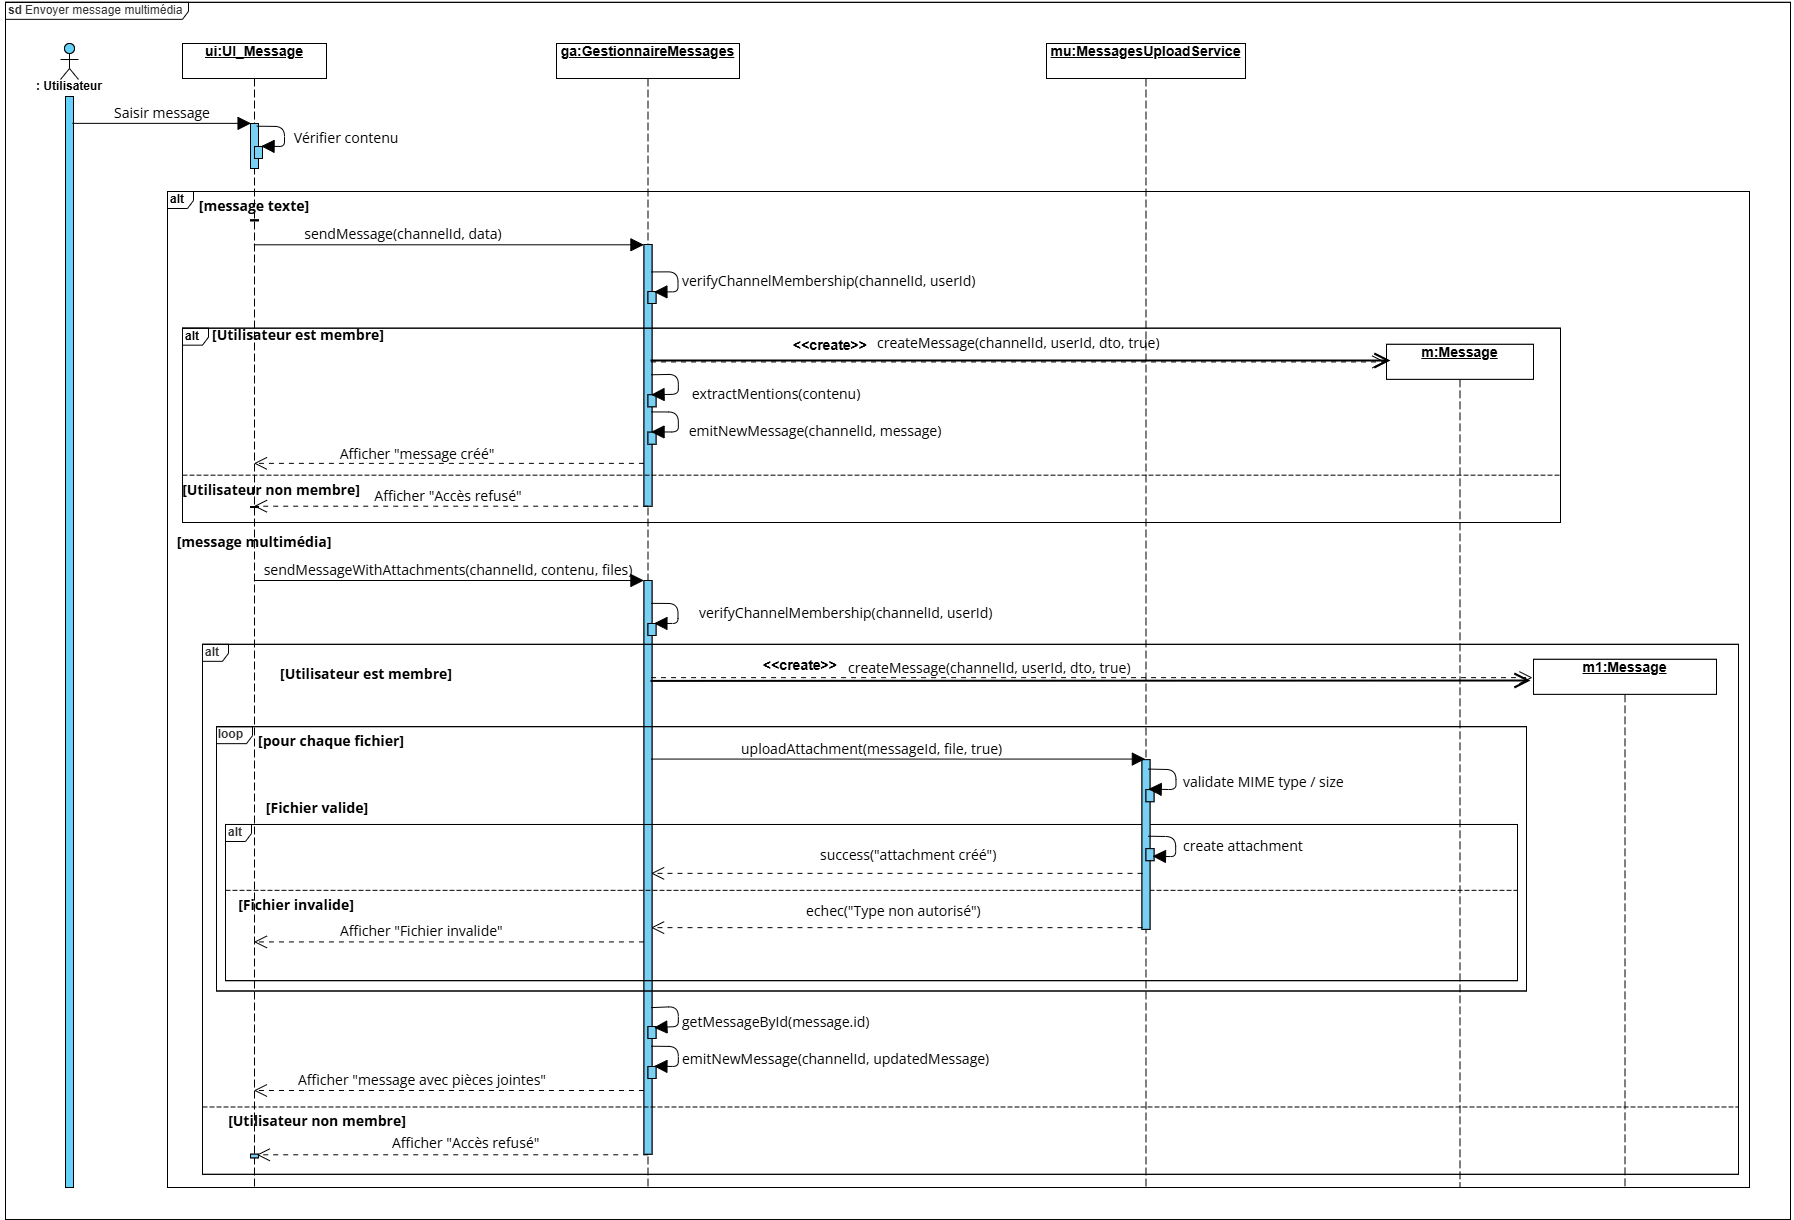
\includegraphics[width=0.85\textwidth,height=0.75\textheight,keepaspectratio]{Images/diag_seq_envoyer_message.png}
        \caption{Diagramme de séquences du cas d'utilisation « Envoyer message »}
        \label{fig:seq_envoyer_message}
\end{figure}

\subsubsection{Diagramme de séquences du cas d'utilisation « Déposer document »}

\begin{figure}[H]
        \centering
       % \includegraphics[width=0.85\textwidth,height=0.75\textheight,keepaspectratio]{Images/diag_seq_deposer_document.png}
        \caption{Diagramme de séquences du cas d'utilisation « Déposer document »}
        \label{fig:seq_deposer_document}
\end{figure}

\subsection{Diagramme de composants}

La figure ci-dessous présente le diagramme de composants de l'application.

\begin{figure}[H]
\centering
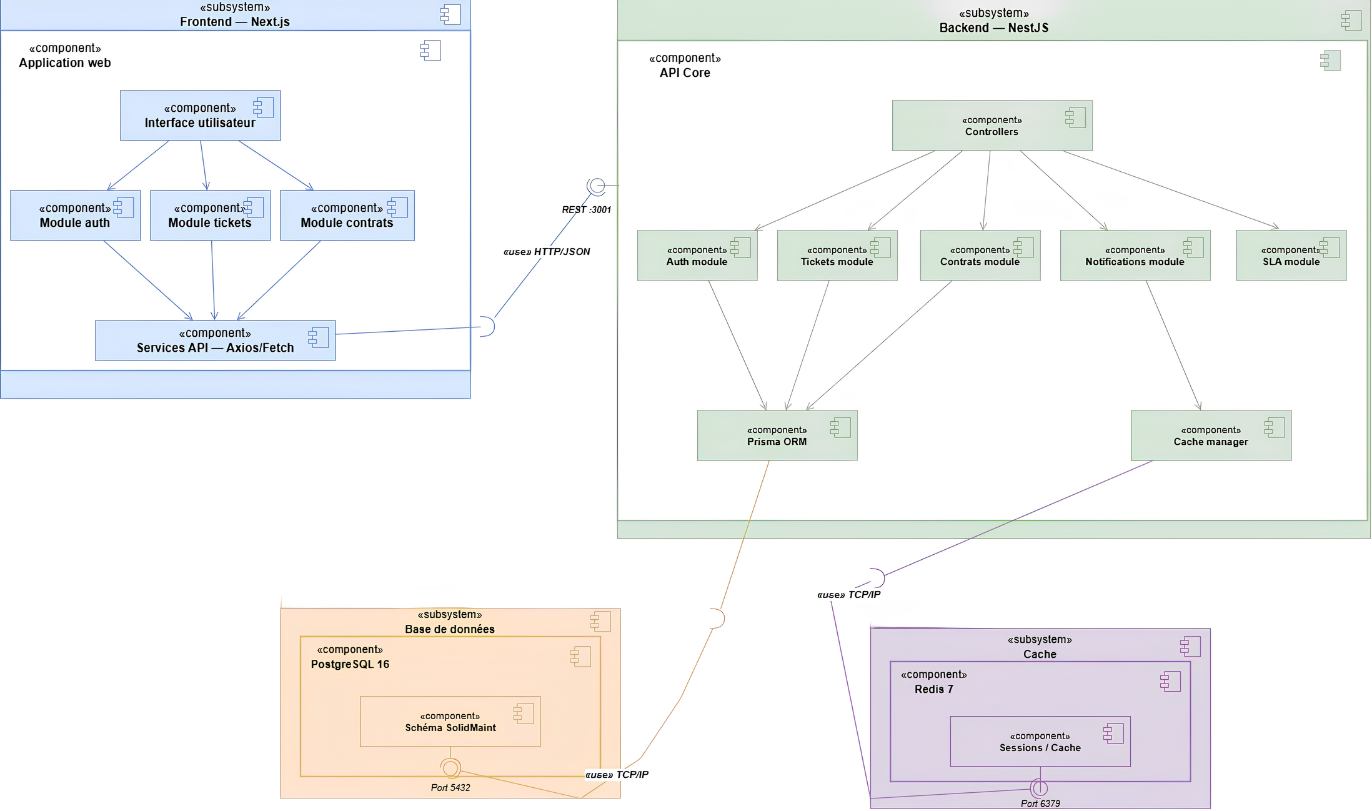
\includegraphics[width=0.95\textwidth,keepaspectratio]{Images/diag comp.png}
\caption{Diagramme de composants de l'application}
\label{fig:diagramme_composants_sprint4}
\end{figure}

Le diagramme de composants illustre l'architecture de la solution en trois couches. Le front-end (Next.js) regroupe l'interface utilisateur, les modules métiers et un client HTTP (Axios/Fetch). L'API Core (NestJS) structure ses contrôleurs, modules fonctionnels et services transverses (Prisma ORM, cache manager). En infrastructure, PostgreSQL assure la persistance des données et Redis gère les sessions et le cache, tous deux accessibles via TCP/IP. Cette organisation sépare clairement la présentation, la logique métier et les services d'infrastructure.

\subsection{Diagramme de classes du quatrième sprint}

\begin{figure}[H]
\centering
%\includegraphics[width=1\textwidth,keepaspectratio]{Images/diag classe sprint 4.png}
\caption{Diagramme de classes du quatrième sprint}
\label{fig:diag_classe_sprint4}
\end{figure}

\section{Schéma relationnel}
{\sloppy
Nous présentons ci-dessous le schéma relationnel réalisé pour ce sprint, qui détaille les différentes tables de la base de données ainsi que leurs relations :

\noindent

\textbf{Canal} (\underline{idCanal}, nomCanal, typeCanal, description, dateCreation, dateMiseAJour, \textbf{\#idContrat}, \textbf{\#idTicket})
\newline
\textbf{Message} (\underline{idMessage}, contenu, dateEnvoi, dateModification, estSupprime, \textbf{\#idCanal}, \textbf{\#idExpediteur}, \textbf{\#idMessageParent})
\newline
\textbf{PieceJointeMessage} (\underline{idPieceJointe}, nomFichier, urlFichier, typeFichier, tailleFichier, dateCreation, \textbf{\#idMessage})
\newline
\textbf{MentionMessage} (\underline{idMention}, estLue, dateCreation, \textbf{\#idMessage}, \textbf{\#idUtilisateurMentionne})
\newline
\textbf{Document} (\underline{idDocument}, nomDocument, urlFichier, typeDocument, tailleFichier, versionCourante, estArchive, dateDepot, dateMiseAJour, \textbf{\#idDeposeur}, \textbf{\#idTicket}, \textbf{\#idContrat})
\newline
\textbf{VersionDocument} (\underline{idVersion}, numeroVersion, urlFichier, tailleFichier, dateCreation, \textbf{\#idDocument}, \textbf{\#idAuteur})
\newline
\textbf{ConsultationDocument} (\underline{idConsultation}, dateConsultation, \textbf{\#idDocument}, \textbf{\#idUtilisateur})
\newline
\textbf{Notification} (\underline{idNotification}, titre, message, typeNotification, estLue, dateCreation, donneesContexte, \textbf{\#idUtilisateur})
\newline
\textbf{PreferenceNotification} (\underline{idPreference}, typeEvenement, canalEmail, canalPush, canalInApp, canalSlack, \textbf{\#idUtilisateur})
\newline
\textbf{AbonnementPush} (\underline{idAbonnement}, endpoint, cleP256dh, cleAuth, dateCreation, \textbf{\#idUtilisateur})

}

% ─────────────────────────────────────────────────────────────────────────────
% SECTION 4 : RÉALISATION
% ─────────────────────────────────────────────────────────────────────────────

\section{Réalisation}
\label{sec:realisation_sprint4}

\subsection{Architecture technique}

Cette section présentera l'architecture technique mise en place pour le Sprint 4, incluant les modules de messagerie temps réel, gestion documentaire et tableaux de bord.

\textit{[À compléter avec les détails d'implémentation]}

\subsection{Interfaces utilisateur}

Cette section présentera les principales interfaces développées durant le Sprint 4, notamment la messagerie, le calendrier, les tableaux de bord et le système de notifications.

\textit{[À compléter avec les captures d'écran]}

\newpage

% ─────────────────────────────────────────────────────────────────────────────
% SECTION 5 : TESTS
% ─────────────────────────────────────────────────────────────────────────────

\section{Tests}
\label{sec:tests_sprint4}

\subsection{Tests unitaires}

Cette section présentera les tests unitaires réalisés pour valider les fonctionnalités du Sprint 4.

\textit{[À compléter avec les résultats des tests]}

\subsection{Tests d'intégration}

Cette section présentera les tests d'intégration effectués pour s'assurer du bon fonctionnement global du système.

\textit{[À compléter avec les résultats des tests]}

\subsection{Tests End-to-End (E2E)}

Cette section présentera les tests End-to-End simulant les parcours utilisateurs complets pour les fonctionnalités de messagerie, de gestion documentaire et de notifications.

\textit{[À compléter avec les résultats des tests]}

\newpage

% ─────────────────────────────────────────────────────────────────────────────
% CONCLUSION DU CHAPITRE
% ─────────────────────────────────────────────────────────────────────────────

\section*{Conclusion}

Ce chapitre a présenté le développement du quatrième et dernier sprint de la plateforme \textbf{SolidMaint}. Nous avons mis en place les fonctionnalités transversales qui complètent et enrichissent l'expérience utilisateur : un calendrier de planification offrant une vue synthétique des interventions dans le temps, des tableaux de bord personnalisés par rôle permettant de piloter l'activité et de générer des rapports d'analyse, un module de messagerie interne en temps réel facilitant la collaboration entre les membres de l'équipe, un espace documentaire centralisé garantissant la traçabilité et le versioning des fichiers, ainsi qu'un système de notifications multicanaux assurant que chaque acteur est informé au bon moment.
\newline
L'ensemble de ces fonctionnalités complète le cycle de vie de la gestion de la maintenance, depuis la soumission d'une demande client jusqu'à la clôture du ticket, en passant par toutes les étapes de collaboration, de coordination et de suivi. La plateforme \textbf{SolidMaint} constitue ainsi une solution de gestion de la maintenance applicative complète, intégrée et orientée vers l'efficacité opérationnelle des équipes techniques.

\cleardoublepage
\newpage
\thispagestyle{fancy}
\phantomsection
\addcontentsline{toc}{chapter}{Conclusion générale}
\mtcaddchapter
\markboth{Conclusion générale}{Conclusion générale}

% Titre dans un cadre centré, sur la même page
\begin{center}
\vspace*{0.5cm}
\begin{tikzpicture}
  \node[
    draw        = primary,
    line width  = 0.8pt,
    fill        = white,
    inner xsep  = 2.0cm,
    inner ysep  = 0.7cm,
    text width  = 10cm,
    align       = center
  ]{
    {\fontsize{16}{20}\selectfont\bfseries\scshape\rmfamily\color{primary}
    Conclusion générale}
  };
\end{tikzpicture}
\vspace{0.8cm}
\end{center}

\justifying
À travers ce projet de fin d'études réalisé au sein de \textbf{SolidWall Consulting}, nous avons conçu et développé \textbf{SolidMaint}, une plateforme web de gestion des contrats de maintenance visant à centraliser et automatiser l'ensemble des processus métier de l'entreprise.

\medskip

Ce travail nous a conduits à parcourir toutes les étapes d'un projet logiciel complet : de l'analyse de l'existant et la spécification des besoins, à la modélisation UML, jusqu'à la réalisation et la validation par les tests. Structuré en quatre sprints selon la méthodologie \textbf{Scrum}, le développement a permis de couvrir progressivement l'ensemble du cycle de vie d'une demande de maintenance, depuis sa soumission jusqu'à sa clôture.

\medskip

Sur le plan \textbf{académique}, ce projet nous a permis d'atteindre une maturité supplémentaire en abordant des problématiques d'une complexité inédite, notamment la conception d'une architecture modulaire, l'intégration de l'intelligence artificielle et la mise en place d'une stratégie de tests complète.

\medskip

Sur le plan \textbf{personnel}, cette expérience a représenté une étape importante dans notre parcours en nous confrontant aux réalités du monde professionnel : adapter nos décisions aux contraintes du terrain, communiquer efficacement avec les différentes parties prenantes et assumer la responsabilité d'un produit destiné à un usage réel.

\medskip

En perspective, plusieurs axes d'amélioration pourraient être envisagés, notamment le déploiement sur une infrastructure cloud pour garantir une haute disponibilité, le développement d'une application mobile pour une accessibilité élargie, ainsi que l'enrichissement des capacités d'intelligence artificielle vers une analyse prédictive des incidents récurrents.
\newpage
\chapter*{Webographie}
\addcontentsline{toc}{chapter}{Webographie}
\mtcaddchapter
\markboth{Webographie}{Webographie}
\hypersetup{urlcolor=primary}

{\color{primary}
\noindent
\label{ref:1}{[1]} - \url{https://solidwall.com.tn/} \hfill Consulté le 03 février 2026
\newline
\label{ref:2}{[2]} - \url{https://www.linkedin.com/posts/solid-wall-consulting_pfe-book-2026-2026-activity-7402287392465862656-MR2f} \hfill Consulté le 05 février 2026
\newline
\label{ref:3}{[3]} - \url{https://agilemanifesto.org/} (Agile Manifesto, 2001) \hfill Consulté le 01 juin 2026
\newline
\label{ref:4}{[4]} - \url{https://www.omg.org/uml/why-uml-is-important.htm} \hfill Consulté le 14 février 2026
\newline
\label{ref:5}{[5]} - \url{https://miro.com/fr/planification-strategique/qu-est-ce-qu-un-diagramme-de-gantt/} \hfill Consulté le 18 février 2026
\newline
\label{ref:6}{[6]} - \url{https://docs.nestjs.com} \hfill Consulté le 22 février 2026
\newline
\label{ref:7}{[7]} - \url{https://nextjs.org/docs} \hfill Consulté le 25 février 2026
\newline
\label{ref:8}{[8]} - \url{https://react.dev} \hfill Consulté le 27 février 2026
\newline
\label{ref:9}{[9]} - \url{https://tailwindcss.com} \hfill Consulté le 02 mars 2026
\newline
\label{ref:10}{[10]} - \url{https://ui.shadcn.com/docs} \hfill Consulté le 05 mars 2026
\newline
\label{ref:11}{[11]} - \url{https://code.visualstudio.com/docs} \hfill Consulté le 08 mars 2026
\newline
\label{ref:12}{[12]} - \url{https://about.gitlab.com} \hfill Consulté le 11 mars 2026
\newline
\label{ref:13}{[13]} - \url{https://www.omg.org/uml} \hfill Consulté le 14 mars 2026
\newline
\label{ref:14}{[14]} - \url{https://www.lucidchart.com} \hfill Consulté le 17 mars 2026
\newline
\label{ref:15}{[15]} - \url{https://swagger.io} \hfill Consulté le 20 mars 2026
\newline
\label{ref:16}{[16]} - \url{https://www.prisma.io/docs} \hfill Consulté le 23 mars 2026
\newline
\label{ref:17}{[17]} - \url{https://www.postgresql.org} \hfill Consulté le 26 mars 2026
\newline
\label{ref:18}{[18]} - \url{https://redis.io/docs} \hfill Consulté le 29 mars 2026
\newline
\label{ref:19}{[19]} - \url{https://neon.tech/docs} \hfill Consulté le 01 avril 2026
\newline
\label{ref:20}{[20]} - \url{https://docs.docker.com} \hfill Consulté le 05 avril 2026
\newline
\label{ref:21}{[21]} - \url{https://owasp.org/about/} \hfill Consulté le 09 avril 2026
\newline
\label{ref:22}{[22]} - \url{https://grafana.com/docs/k6/latest/} \hfill Consulté le 13 avril 2026
\newline
\label{ref:23}{[23]} - \url{https://www.notion.so} \hfill Consulté le 17 avril 2026
\newline
\label{ref:24}{[24]} - \url{https://www.latex-project.org} \hfill Consulté le 21 avril 2026
\newline
\label{ref:25}{[25]} - \url{https://www.canva.com} \hfill Consulté le 25 avril 2026
\newline
\label{ref:26}{[26]} - \url{https://vitest.dev} \hfill Consulté le 17 avril 2026
\newline
\label{ref:27}{[27]} - \url{https://playwright.dev} \hfill Consulté le 21 avril 2026
\newline
\label{ref:28}{[28]} - \url{https://glpi-project.org/} \hfill Consulté le 25 avril 2026
\newline
\label{ref:29}{[29]} - \url{https://freshdesk.com/} \hfill Consulté le 25 avril 2026
\newline
\label{ref:30}{[30]} - \url{https://www.atlassian.com/software/jira/service-management} \hfill Consulté le 25 avril 2026
\newline
\label{ref:31}{[31]} - \url{https://scrumguides.org/scrum-guide.html} (Édition novembre 2020, Ken Schwaber et Jeff Sutherland) \hfill Consulté le 01 juin 2026
\newline
\label{ref:32}{[32]} -  \url{https://ebooks.karbust.me/Technology/Agile.Software.Development.Principles.Patterns.and.Practices.Pearson.pdf} \hfill Consulté le 05 juin 2026
\newline
\label{ref:33}{[33]} - \url{https://lecoursgratuit.com/qcm-gestion-de-projet-informatique/} \hfill Consulté le 09 juin 2026
\newline

\end{document}